% Platzhalter


% Variablen

% Titel der Abschlussarbeit
\newcommand{\myTitle}{Barrierefreiheit in Virtual Reality – Konzeption, Implementierung und Evaluation von binären Interaktionsschnittstellen in PaneoVR für Nutzende mit motorischen Einschränkungen}

% Vor- und Nachname
\newcommand{\myAuthor}{Finja Wegener}

% Datum der Abgabe
\newcommand{\myDate}{16. Januar 2025}

% Ort
\newcommand{\myOrt}{Lübeck}

% Matrikelnummer
\newcommand{\myMatrikelnummer}{311854}

%%%%%%%%%%%%%%%%%%%%%%%%%%%%%%%%%%%%%%%%%%%%%%%%%%%%%%%%%%%%%%%%%%%%%%

\documentclass
[
    ngerman,
    headsepline, % Linie in Kopfzeile
    automark,
    listof=totoc, % Verzeichnisse im Inhaltsverzeichnis aufführen
    bibliography=totoc, % Literaturverzeichnis im Inhaltsverzeichnis aufführen
    oneside, % Einseitig
    appendixprefix, % Das Wort "Anhang" vor dem Buchstabe des Anhangs ergänzen
    numbers=noenddot, % Kein Punkt nach Kapitelnummer
    parskip
]
{scrbook}

% Laden der Pakete
\usepackage[utf8]{inputenc}
\usepackage[T1]{fontenc}
\usepackage{lmodern}

% glqq
\usepackage[ngerman]{babel}

% Required for inserting images
\usepackage{graphicx}

% Beliebige Schriftgrößen verwenden
% https://ctan.org/pkg/anyfontsize
\usepackage{anyfontsize}

\usepackage{scrlayer-scrpage}

% Layout von itemize, enumerate und description anpassen
% https://ctan.org/pkg/enumitem
\usepackage{enumitem}

% Verwenden von \theauthor etc.
%\usepackage{titling}

% Muss vor Package natbib geladen werden
\usepackage{apacite}

% Für cite
\usepackage{natbib}
\usepackage{citeref}
%\usepackage{varioref}

\usepackage{hyperref}


% Muss nach Package hyperref geladen werden
\usepackage[acronym,toc]{glossaries}

% Code
\usepackage{listings}

% Einfärben der Hyperlinks, anstelle der Boxen...
\usepackage{xcolor}
\hypersetup{
    colorlinks,
    linkcolor={red!50!black},
    citecolor={blue!50!black},
    urlcolor={blue!80!black}
}


\clearpairofpagestyles

% Anpassen der Kopfzeile: Kapitel links, Seitenzahl rechts
\ihead[]{\headmark}
\ohead[]{\pagemark}

\pagestyle{scrheadings}

% Kopfzeile auch auf Seiten, auf denen ein Kapitel anfängt
\renewcommand*\chapterpagestyle{scrheadings}

% Grafikordner auf "images/" setzen
\graphicspath{{images/}}

% New colors defined below
\definecolor{codegreen}{rgb}{0,0.6,0}
\definecolor{codegray}{rgb}{0.5,0.5,0.5}
\definecolor{codepurple}{rgb}{0.58,0,0.82}
\definecolor{backcolour}{rgb}{0.95,0.95,0.92}

% Code listing style named "mystyle"
\lstdefinestyle{mystyle}{
  backgroundcolor=\color{backcolour},
  commentstyle=\color{codegreen},
  keywordstyle=\color{magenta},
  numberstyle=\tiny\color{codegray},
  stringstyle=\color{codepurple},
  basicstyle=\ttfamily\footnotesize,
  breakatwhitespace=false,         
  breaklines=true,                 
  captionpos=b,                    
  keepspaces=true,                 
  numbers=left,                    
  numbersep=5pt,                  
  showspaces=false,                
  showstringspaces=false,
  showtabs=false,                  
  tabsize=2
}

\lstset{style=mystyle}


\newacronym{gcd}{GCD}{Greatest Common Divisor}

\newacronym{lcm}{LCM}{Least Common Multiple}

\newglossaryentry{maths}
{
    name=mathematics,
    description={Mathematics is what mathematicians do}
}

\newglossaryentry{latex}
{
    name=latex,
    description={Is a markup language specially suited for scientific documents}
}

\newglossaryentry{formula}
{
    name=formula,
    description={A mathematical expression}
}


\makeglossaries

\begin{document}

% Anfang des Dokuments
\frontmatter

\begin{titlepage}

\begin{center}

\begin{figure}[tbh]
 \centering
 
\includegraphics[width=0.5\textwidth]{images/th-logo.png}
\end{figure}

\vspace{1.cm}

{
 \fontsize{20}{28}\selectfont
 \myTitle\\[0.5cm]
}

\fontsize{12}{12}\selectfont

\vspace{1.cm}

Masterarbeit\\
zur Erlangung des akademischen Grades M.Sc.\\
im Studiengang Medieninformatik\\
des Fachbereichs Elektrotechnik und Informatik\\
an der Technischen Hochschule Lübeck

\vspace{0.5cm}

Eingereicht von:\\
\myAuthor\\
Matrikelnummer: \myMatrikelnummer

\vspace{0.5cm}

Erstprüfer:\\
Prof. Dr. Thies Pfeiffer\\
Hochschule Emden/Leer\\


\vspace{.3cm}

Zweitprüfer:\\
Dr. Daniel Sacristán\\
Technische Hochschule Lübeck\\


\vspace{0.5cm}

Ausgabe: \startDate\\
Abgabe: \myDate

\end{center}
\end{titlepage}


\cleardoublepage

% Römische Zahlen in Groß
\pagenumbering{Roman}

\chapter{Abstract}

Kurzfassung auf Englisch.

\chapter{Kurzfassung}

Diese Arbeit untersucht die Entwicklung binärer Interaktionsschnittstellen für Virtual Reality (VR) Anwendungen mit dem Ziel, die Zugänglichkeit für Menschen mit motorischen Beeinträchtigungen zu verbessern. Auf Basis einer strukturierten Konzeption wurden zwei Ansätze entwickelt, die auf den etablierten Scanning-Verfahren Automatic Item Scanning und Continuous Cartesian Scanning basieren und gezielt für den Einsatz in VR adaptiert wurden. Beide Ansätze wurden prototypisch auf Basis des Tools PaneoVR implementiert.

Die anschließende Evaluation der implementierten Schnittstellen untersuchte die Unterschiede hinsichtlich Effizienz, Erlernbarkeit, Robustheit, Usability, User Experience (UX) und dem Auftreten von Motion Sickness. Die Ergebnisse zeigen, dass das Item Scanning durch technische Vorteile wie eine höhere Interaktionsgeschwindigkeit und Robustheit überzeugt, während das Cartesian Scanning in den subjektiven Bewertungen, insbesondere in Bezug auf Usability und UX, positiver wahrgenommen wird.
Beide Ansätze zeigen spezifische Stärken und Schwächen. Auf Basis der Evaluation wurden konkrete Verbesserungsansätze abgeleitet und Empfehlungen für die Entwicklung binärer Interaktionsschnittstellen in VR-Anwendungen formuliert. Zu diesen Empfehlungen gehören u. a. die Implementierung unterschiedlicher Scanning-Verfahren, die Integration effizienter Mechanismen zur Fehlerkorrektur sowie die ergonomische Platzierung von UI- und Interaktionselementen.
Eine zentrale Limitation der Ergebnisse besteht in der fehlenden zielgruppenspezifischen Evaluation, wodurch die Übertragbarkeit der Ergebnisse auf Menschen mit motorischen Beeinträchtigungen eingeschränkt ist. Zukünftige Arbeiten sollten die identifizierten Verbesserungsansätze umsetzen und durch zielgruppenspezifische Untersuchungen validieren. Die gewonnenen Erkenntnisse leisten einen Beitrag zur Entwicklung inklusiver VR-Anwendungen und tragen zur Verbesserung der Barrierefreiheit für Menschen mit motorischen Beeinträchtigungen bei.
\chapter{Danksagung}

Danke an …


\tableofcontents
\listoffigures
\listoftables
\printglossary[type=\acronymtype,title=Abkürzungsverzeichnis]
\printglossary[title=Glossar]

\cleardoublepage

%\pagenumbering{arabic}

% Hauptteils des Dokuments
\mainmatter

\chapter{Einleitung}

Motorische Beeinträchtigungen umfassen den Verlust oder die Einschränkung der Fähigkeit, Muskeln oder Bewegungen zu kontrollieren, und betreffen zahlreiche Menschen weltweit. Die Ursachen sind vielfältig und reichen von Arthritis und Lähmungen bis hin zu neurologischen Erkrankungen wie Zerebralparese oder Verletzungen durch wiederholte Belastung \citep{yuan_game_2011}. Solche Beeinträchtigungen wirken sich nicht nur auf die Mobilität der Personen aus, sondern können auch den Zugang zu digitalen Technologien erschweren. Die Gestaltung barrierefreier Systeme zielt entsprechend darauf ab, Produkte und Anwendungen so zu entwickeln, dass sie von einer möglichst breiten Nutzergruppe mit unterschiedlichen Anforderungen, Fähigkeiten und Fertigkeiten verwendetet werden können. Dies umfasst auch die Berücksichtigung spezifischer Nutzungskontexte, einschließlich der Unterstützung assistiver Technologien \citep{DINISO9241}. 

Virtual Reality (VR) bietet ein wachsendes Spektrum an Anwendungen, von Bildung und Medizin bis hin zu Entertainment und Training. Mit zunehmend erschwinglicher Hardware ist VR nicht mehr nur ein Nischenprodukt, sondern eine Technologie, die für den Consumer-Bereich zunehmend attraktiv wird. Diese Entwicklung eröffnet auch für Menschen mit gesundheitlichen Beeinträchtigungen neue Möglichkeiten. Insbesondere für Personen mit motorischen Beeinträchtigungen könnte VR eine Plattform bieten, die neue Formen der Interaktion und Teilhabe ermöglicht \citep{10.1145/3373625.3416998}.

In Bezug auf die Barrierefreiheit weist VR jedoch eine gewisse Rückständigkeit im Vergleich zu anderen Technologien auf. Während gängige Betriebssysteme für Smartphones oder Computer bereits umfangreiche Tools zur Barrierefreiheit für Menschen mit unterschiedlichen Beeinträchtigungen integriert haben (vgl. z. B. \citep{apple_einfuhrung_2024-2}), fehlen im Bereich VR weithin standardisierte Richtlinien und Werkzeuge \citep{ciccone_next_2023}. Aus dieser Lücke in der Barrierefreiheit resultiert nicht nur eine technische Herausforderung, sondern auch die gesellschaftliche Notwendigkeit, sicherzustellen, dass technologische Fortschritte allen Menschen zugänglich gemacht werden.

\section{Motivation}

Die Entwicklung inklusiver VR-Anwendungen wird durch vier grundlegende Faktoren motiviert. (1) Besonders hervorzuheben ist das ethische und moralische Anliegen, technologische Fortschritte allen Menschen zugänglich zu machen. (2) Darüber hinaus hat sich gezeigt, dass VR-Technologie ein erhebliches Potenzial besitzt, Barrieren in den Bereichen Rehabilitation und Assistenztechnologien abzubauen und somit die Lebensqualität von Menschen zu verbessern. Dies bietet insbesondere für Menschen mit Beeinträchtigungen eine vielversprechende Perspektive. (3) Zusätzlich bringt die Ansprache einer größeren Nutzergruppe auch kommerzielle Vorteile mit sich, da sie den Zugang zu einem breiteren Markt und größeren Absatzchancen ermöglicht. (4) Schließlich führt ein barrierefreies Design häufig zu einer verbesserten Usability für alle Nutzenden. Dieser Aspekt ist besonders relevant im Hinblick auf situationale Einschränkungen, die auftreten, wenn äußere Umstände die Fähigkeit einer Person beeinträchtigen, bestimmte Aktivitäten auszuführen \citep{10.1145/1952383.1952384}. Auch Personen ohne dauerhafte Beeinträchtigungen können von solchen situationalen Einschränkungen betroffen sein, etwa bei der Nutzung in beengten Räumen oder bei temporären Verletzungen. Ein inklusives Design, das die Bedürfnisse von Menschen mit dauerhaften Einschränkungen berücksichtigt, verbessert somit auch die Nutzungserfahrung für situativ eingeschränkte Personen \citep{dudley_inclusive_2023}.

In der Forschung zur Barrierefreiheit in VR wird zunehmend betont, dass die individuellen Bedürfnisse der Endnutzenden im Zentrum der Entwicklung stehen müssen \citep{10.1007/978-3-030-21607-8_3}. Um für Menschen mit motorischen Beeinträchtigungen dieses Ziel zu erreichen, ist die Entwicklung binärer Interaktionsschnittstellen, die auf einfache Steuerungsmöglichkeiten reduziert sind, ein vielversprechender Ansatz.
Diese erfordern minimale körperliche Anstrengung und ermöglichen damit einer breiten Nutzergruppe den Zugang zu VR-Anwendungen. Solche Schnittstellen bieten nicht nur eine Lösung für Menschen mit motorischen Beeinträchtigungen, sondern verbessern auch die Nutzbarkeit von Systemen in Situationen, in denen physische Bewegungen eingeschränkt oder unpraktisch sind, beispielsweise in beengten Räumen oder bei anderen situationalen Einschränkungen \citep{10.1145/1952383.1952384}.

\section{Zielsetzung}

Um Menschen mit motorischen Beeinträchtigungen die Nutzung der Anwendung PaneoVR zu ermöglichen, besteht das Ziel dieser Arbeit in der Konzeption und prototypischen Implementierung zweier binärer Interaktionsschnittstellen. Dadurch sollen mit PaneoVR erstellte VR-Trainings auch für diese Zielgruppe zugänglich und erlebbar werden.

Um eine möglichst barrierearme Nutzung zu gewährleisten, umfasst die Zielsetzung sowohl die Entwicklung eines geeigneten Interfaces als auch die systematische und detaillierte Konzeption der Interaktionen. Eine zentrale Anforderung dabei ist, dass alle erforderlichen Interaktionen mit dem System durch eine binäre Eingabe, bspw. über einen Schalter, ausgeführt werden können. Die implementierten Interaktionsformen sollen anschließend umfassend evaluiert werden und die gewonnenen Erkenntnisse dazu beitragen, Empfehlungen für die Entwicklung barrierearmer VR-Anwendungen abzuleiten.

Zur strukturierten Bearbeitung und Präzisierung dieser Zielsetzung wurden konkret folgende Forschungsfragen definiert, die im Rahmen dieser Arbeit beantwortet werden sollen:

\begin{itemize}
    \item FF1: Wie können binäre Interaktionen in Virtual Reality gestaltet werden, um die Zugänglichkeit für Personen mit motorischen Beeinträchtigungen zu verbessern?
    \item FF2: Welche Herausforderungen treten bei der Implementierung binärer Interaktionsschnittstelle auf und wie können diese überwunden werden?  
    \item FF3: Welche Unterschiede hinsichtlich Faktoren wie Effizienz, Robustheit, Usability und User Experience zeigen sich zwischen den entwickelten Ansätzen? Stimmen diese Ergebnisse mit den Erwartungen aus der Konzeption überein? Ist eine der implementierten Interaktionsformen geeigneter für die Verwendung in VR?
    \item FF4: Welche Empfehlungen können aus der Implementierung und Evaluation der binären Interaktionsschnittstellen in PaneoVR für die Entwicklung barrierearmer VR-Anwendungen abgeleitet werden?
\end{itemize}
 

\section{Aufbau der Arbeit}

Im Verlauf dieser Arbeit werden die aufgestellten Forschungsfragen systematsich in den einzelnen Kapitel adresseirt. Zunächst wird eine inhaltliche Grundlage geschaffen. Hierbei werden relevante theoretische und technologische Konzepte sowie der aktuelle Forschungsstand im Bereich barrierearmer Interaktionsschnittstellen und VR dargestellt (\autoref{chap:2Stand}). Dieser Überblick dient als Basis für die weitere Arbeit und ermöglicht ein umfassendes Verständnis der Thematik.

Darauffolgend wird im Rahmen der Konzeption die Forschungsfrage FF1 addressiert (\autoref{chap:Konzept}). Hier liegt der Fokus auf der Gestaltung der beiden binären Interaktionsschnittstellen. Zunächst wird ein Design Space definiert, der die Gestaltungsmöglichkeiten und Anforderungen beschreibt. Auf dieser Grundlage werden konkrete Ausprägungen für Interaktionsaufgaben und -komponenten erarbeitet. Diese Ausprägungen werden anschließend systematisch anhand relevanter Parameter bewertet, um die Designentscheidungen nachvollziehbar darzulegen und zu begründen. Abschließend werden die finalen Konzepte für die beiden Interaktionsschnittstellen abgeleitet.

Anschließend wird die technische Umsetzung der entwickelten Konzepte beschrieben (\autoref{chap:Implementierung}). Neben der Vorstellung der Implementierung werden auch die Herausforderungen bei der Realisierung der binären Interaktionsschnittstellen thematisiert (FF2).

Im Anschluss werden zunächst Konzeption, Aufbau und Durchführung der Evaluation dargestellt, gefolgt von der Präsentation der Ergebnisse (\autoref{chap:Evaluation}).

Diese Ergebnisse werden daraufhin umfassend eingeordnet und interpretiert (\autoref{chap:Diskussion}). Dabei liegt ein besonderer Fokus auf dem Vergleich der beiden Interaktionsschnittstellen hinsichtlich Faktoren wie Effizienz, Robustheit, Usability, User Experience und Motion Sickness. Es wird untersucht, ob die erzielten Ergebnisse mit den im Vorfeld formulierten Erwartungen übereinstimmen und ob eine der entwickelten Interaktionsschnittstellen besser für den Einsatz in VR geeignet ist (FF3). Zudem werden Stärken, Schwächen und mögliche Verbesserungsansätze der Interaktionsschnittstellen aufgezeigt und Empfehlungen für die Entwicklung binärer Interaktionsschnittstellen abgeleitet (FF4). 

Abschließend werden die zentralen Ergebnisse der Arbeit zusammengefasst und mögliche Perspektiven für weiterführende Forschung aufgezeigt (\autoref{chap:Fazit}).

\chapter{Stand der Forschung}
\label{chap:2Stand}
%TO DOs für dieses Kapitel: Abbildung optimieren und einfügen, ergänzen: Wie bin ich bei der Literaturrecherche vorgegangen; Kommentare Rafael 

Dieses Kapitel legt die Grundlage für ein umfassendes Verständnis der Arbeit, indem relevante theoretische und technologische Konzepte sowie der aktuelle Forschungsstand dargestellt werden. Zunächst werden die Grundlagen von Virtual Reality erläutert, einschließlich der Definition von Virtual Reality und zentraler Begriffe wie Immersion und Presence. Zudem erfolgt eine Abgrenzung zu verwandten Begriffen und Konzepten wie Augmented Reality und Mixed Reality. Ergänzend werden grundlegende Informationen zu VR-Ausgabegeräten bereitgestellt, die eine technische Basis für das Verständnis der nachfolgenden Inhalte schaffen. Ein besonderer Schwerpunkt liegt auf dem Phänomen der Motion Sickness, da das Auftreten körperlicher Symptome eine häufige Herausforderung bei der Nutzung von VR-Anwendungen darstellt. 
Im weiteren Verlauf widmet sich das Kapitel dem aktuellen Forschungsstand zur Barrierefreiheit in VR. Zunächst werden bestehende Richtlinien vorgestellt. Anschließend werden Barrieren beleuchtet, die Menschen mit motorischen Beeinträchtigungen bei der Nutzung von VR-Anwendungen erfahren, und bestehende Lösungsansätze zur Überwindung dieser Barrieren präsentiert. Dabei wird auch auf Bereiche mit weiterem Forschungsbedarf hingewiesen.
Ein weiterer Abschnitt behandelt binäre Interaktionsschnittstellen als spezifische Lösung zur Verbesserung der Zugänglichkeit für Menschen mit motorischen Beeinträchtigungen. Hierbei werden zunächst verschiedene Arten von Schaltern beschrieben und anschließend gängige Scanning-Verfahren erläutert, die die Nutzung dieser Schalter ermöglichen.
Die Konzepte Usability und User Experience bilden eine wichtige Grundlage für die Bewertung von VR-Anwendungen. In diesem Zusammenhang werden etablierte Messmethoden wie der System Usability Scale (SUS) und der User Experience Questionnaire (UEQ) vorgestellt.
Anschließend wird das Tool PaneoVR eingeführt, das als Grundlage für die Implementierung der im Rahmen dieser Arbeit erarbeiteten Konzepte dient. Eine Zusammenfassung des Kapitels bietet einen abschließenden Überblick über den Stand der Forschung und leitet über zur Konzeption.

\section{Virtual Reality}

Der Begriff "Virtual Reality (VR)" wird in der Literatur nicht einheitlich definiert \citep{wohlgenannt_virtual_2020}. Es existieren verschiedene Definitionen, die unterschiedliche Aspekte der Technologie betonen. So wird VR beispielsweise von \citet{berg_industry_2017} als eine Sammlung von Technologien beschrieben, die es Menschen ermöglichen, immersiv eine Welt jenseits der Realität zu erleben. 
Nach \citet{bowman_virtual_2007} simuliert VR eine virtuelle Umgebung, die den Nutzenden das Gefühl vermittelt, "dort zu sein". \citet{jerald_vr_2016} definiert VR hingegen als eine computergenerierte digitale Umgebung, die erlebt und interagiert werden kann, als ob diese Umgebung real wäre. In ihrer Definition von VR führen \citet{wohlgenannt_virtual_2020} die verschiedenen Ansätze zur Beschreibung von VR zusammen und präzisieren, dass VR immersive Technologien nutzt, um interaktive virtuelle Umgebungen oder virtuelle Welten zu simulieren, in die sich die Nutzenden subjektiv einbringen und in denen sie sich physisch anwesend fühlen.

Des Weiteren identifizieren \citet{walsh_virtual_2002} Immersion, Interaktivität und Presence als drei zentrale Konzepte von VR. Der Begriff der Presence wird definiert als "die subjektive Erfahrung, sich an einem Ort oder in einer Umgebung zu befinden, auch wenn man physisch an einem anderen Ort ist" \citep{witmer_measuring_1998}. In einer virtuellen Umgebung entsteht das Gefühl von Presence insbesondere durch die Verlagerung der Aufmerksamkeit von der physischen auf die virtuelle Umgebung, wobei jedoch keine vollständige Ablösung von der physischen Realität notwendig ist \citep{witmer_measuring_1998}. 

Im Gegensatz zur Presence ist der Begriff der Immersion weniger eindeutig definiert. \citet{witmer_measuring_1998} beispielsweise definieren Immersion als einen psychologischen Zustand, in dem eine Person sich als umhüllt und in eine Umgebung eingebunden empfindet, die kontinuierliche Reize und Erfahrungen liefert. \citet{sanchez-vives_presence_2005} hingegen definieren Immersion als die technische Fähigkeit eines Systems, eine umfassende und überzeugende Umgebung zu erschaffen, mit der die Nutzenden interagieren können. 
Die Frage, ob Immersion als psychologischer Zustand oder als technische Eigenschaft des Systems zu verstehen ist, wirkt sich maßgeblich auf die Identifikation von Faktoren aus, die einen Einfluss auf die Immersion haben. 
Zu den wesentlichen Einflussfaktoren auf die Immersion zählen gemäß  \citet{sanchez-vives_presence_2005} unter anderem das \textit{Field of View}, die Anzahl der simulierten sensorischen Systeme, die Qualität der Wiedergabe in jeder Sinnesmodalität, die Genauigkeit des Trackings, die Bildfrequenz und die Latenzzeit sowie die Übereinstimmung der simulierten sensorischen Daten mit der eigenen Körperwahrnehmung (Propriozeption). \citet{witmer_measuring_1998} hingegen definieren die Isolation von der physischen Umgebung, die Wahrnehmung der eigenen Einbindung in die virtuelle Umgebung, natürliche Interaktionsmodi sowie die Wahrnehmung der Eigenbewegung als relevante Einflussfaktoren. 

Neben diesen zentralen Konzepten betonen viele Definitionen die Bedeutung einer virtuellen Umgebung oder einer virtuellen Welt im Kontext von VR. Diese beiden Begriffe werden häufig in der Literatur verwendet, unterscheiden sich jedoch in ihrer Bedeutung. \citet{barfield_presence_1995} definieren eine virtuelle Umgebung als softwarebasierte Darstellungen realer (oder imaginierter) Agenten, Objekte und Prozesse sowie eine Mensch-Computer-Schnittstelle zur Darstellung und Interaktion mit diesen Modellen. Eine virtuelle Welt hingegen ist eine spezifische Form einer (multi-user) virtuellen Umgebung, die gemeinsame, simulierte Räume bietet, die von den Bewohnern, die als Avatare repräsentiert werden, bewohnt und gestaltet werden \citep{girvan_what_2018}.

Bei der Betrachtung des Themenbereichs Virtual Reality erfolgt eine häufige Bezugnahme auf verwandte Konzepte wie Mixed Reality oder Augmented Reality. Zur Klassifizierung und Abgrenzung aller Technologien, die Realität und Virtualität vereinen, entwarfen \citet{milgram_augmented_1995} das sogenannte Reality-Virtuality Continuum (RVC) (vgl. \autoref{fig:continuum}). 

\begin{figure}[tbh]
    \centering
    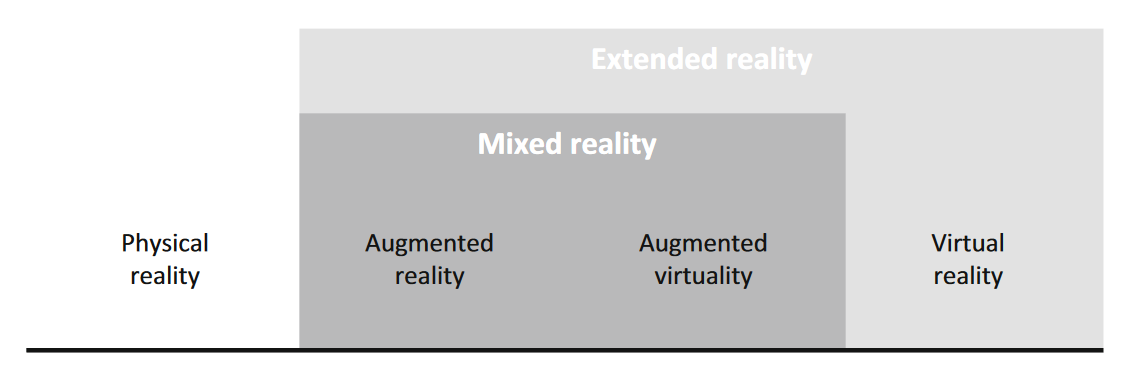
\includegraphics[width=0.95\textwidth]{images/Mixed-Reality-Cont-NEW.png}
    \caption{Reality-virtuality continuum nach \cite{milgram_augmented_1995} in der erweiterten Version von \cite{wohlgenannt_virtual_2020}}
    \label{fig:continuum}
\end{figure}

Auf dem RVC bilden die reale Umgebung und die virtuelle
Umgebung die beiden Pole des Kontinuums. Die physikalische Realität setzt sich ausschließlich aus Elementen zusammen, welche durch eine Person direkt wahrgenommen werden können. Die virtuelle Umgebung, also die VR, besteht ausschließlich aus virtuellen Elementen. Der Nutzende wird dabei von der physikalischen Umgebung abgeschirmt, sodass er vollständig in die virtuelle Umgebung eintauchen kann. Der Bereich, der sich zwischen den beiden Polen des Kontinuums befindet, kombiniert virtuelle und physikalische Elemente und wird als Mixed Reality bezeichnet. Eine Umgebung, in der die physikalischen Elemente überwiegen, wird als Augmented Reality bezeichnet. Hierbei findet eine Erweiterung der physikalischen Realität durch virtuelle Elemente statt. Eine Erweiterung einer virtuellen Umgebung um physikalische Elemente wird demgegenüber als Augmented Virtuality bezeichnet. 
Ein weiterer Begriff, der in diesem Kontext häufig Verwendung findet, ist der Begriff der Extended Reality. Dieser wird häufig als Überbegriff verwendet und erfasst alle realen und virtuellen kombinierten Umgebungen und Mensch-Maschine-Interaktionen, die durch Computertechnologie und tragbare Geräte erzeugt werden \citep{fast-berglund_testing_2018}. \citet{wohlgenannt_virtual_2020} haben daher das ursprüngliche RVC um diesen Begriff erweitert (vgl. \autoref{fig:continuum}). 
 
Um virtuelle Umgebungen für die Nutzenden erfahrbar zu machen, werden sowohl Ausgabegeräte benötigt, die die virtuelle Umgebung darstellen, als auch Eingabegeräte, die die Interaktion mit dieser Umgebung ermöglichen. Ziel der Ausgabegeräte ist es, die virtuelle Welt so darzustellen, dass sie von den Nutzenden möglichst ähnlich wie die reale Welt wahrgenommen werden kann. Zu den am weitesten verbreiteten Ausgabegeräten zählen insbesondere sogenannte Head-Mounted Displays (HMDs). Dabei handelt es sich um Displays, die direkt am Kopf getragen werden und sich direkt vor den Augen der Nutzenden befinden. HMDs verfügen in der Regel über integrierte Trackingsysteme oder werden mit externen Trackinglösungen kombiniert, um die Position und Blickrichtung des Kopfes zu erfassen. Dies ermöglicht eine kontinuierliche Anpassung der virtuellen Kamera an die aktuelle Position und Orientierung des HMDs \citep{dorner_virtual_2019}. Darüber hinaus können aber z. B. auch Immersive Räume, auch CAVE (C-Automatic Virtual Enviroments) genannt, oder große Monitore Ausgabegeräte für VR-Anwendungen sein. Nach \citet{somrak_estimating_2019} können VR-Ausgabegeräte nach folgender Taxonomie beschrieben werden: 

\begin{itemize}
    \item \textbf{Tragbare Geräte:} 
    \begin{itemize}
        \item Mit einem Smartphone als Anzeige- und Verarbeitungseinheit (z. B.  Google Cardboard)
        \item Eigenständige tragbare VR-Geräte (z. B.  Meta Quest 3)
    \end{itemize}
    \item \textbf{Kabelgebundene Geräte:} 
    \begin{itemize}
        \item Geräte mit einer Kabelverbindung zu einem leistungsstarken Computer (z. B.  HTC Vive)
        \item Geräte, die an die Spielkonsole angeschlossen werden können (z. B.  Sony PlayStation VR)
    \end{itemize}
    \item \textbf{Immersive Räume - CAVE}
    \item \textbf{Große Monitore}
\end{itemize}

Die Interaktion mit der virtuellen Umgebung erfolgt in der Regel über spezielle Eingabegeräte. Hier kommen insbesondere VR-Controller zum Einsatz. Alternativ oder ergänzend kann die Eingabe durch direktes Tracking von Körperteilen der Nutzenden, wie z. B.  Finger, Hände, Arme oder Augen, erfolgen. In diesem Fall werden bspw. Gesten erkannt und in der virtuellen Umgebung als Eingaben interpretiert\citep{dorner_virtual_2019}.

\subsection{Motion Sickness}

Das Erleben von VR kann bei Nutzenden Symptome auslösen, die denen von Motion Sickness aus anderen Bereichen ähneln \citep{somrak_estimating_2019}. In der wissenschaftlichen Literatur werden neben dem Begriff "Motion Sickness" verschiedene Begriffe zur Beschreibung von unerwünschten Begleiterscheinungen virtueller Umgebungen verwendet. Dazu gehört der Begriff "Simulator Sickness", der insbesondere in den frühen militärischen Flugsimulatoren geprägt wurde \citep{kennedy_simulator_1993}, sowie "Cybersickness", das ursprünglich die Begleiterscheinungen virtueller Umgebungen allgemein beschrieb \citep{mccauley_cybersickness_1992}. In Studien mit HMDs findet zudem der Begriff "VR-Sickness" Verwendung (z. B.  in \citep{kim_virtual_2018}). In der Forschung zu virtuellen Umgebungen werden diese Begriffe oft synonym verwendet, wobei eine spezifische Abgrenzung nicht erfolgt \citep{saredakis_factors_2020}. Im weiteren Verlauf dieser Arbeit wird der Begriff "Motion Sickness" verwendet. 

Das Spektrum der Symptome von Motion Sickness ist vielfältig. Zu den am häufigsten auftretenden Symptomen zählen unter anderem Unwohlsein, Apathie, Übelkeit, Schläfrigkeit, Desorientierung, Augenbelastung und Müdigkeit \citep{somrak_estimating_2019}. In besonders schweren Fällen können darüber hinaus Symptome wie Erbrechen, Schweißausbrüche, übermäßiger Speichelfluss, Schwindel, Magenschmerzen und völlige Arbeitsunfähigkeit auftreten \citep{kennedy_research_2010}. 

Die genauen Ursachen von Motion Sickness sind bislang nicht vollständig aufgeklärt. Eine der prominentesten Erklärungen liefert die Sensorische Konflikttheorie \citep{oman_motion_1990}. Diese besagt, dass die Symptome durch eine Diskrepanz zwischen visuellen, vestibulären und propriozeptiven Signalen entstehen. Diese Signale dienen in der Regel der Wahrnehmung der Ausrichtung und Bewegung des Körpers. In einer virtuellen Umgebung tritt jedoch häufig der Fall ein, dass der Körper visuell Bewegung wahrnimmt, während die vestibulären und propriozeptiven Systeme keine entsprechende Bewegung registrieren. Diese widersprüchlichen Signale führen zu sensorischen Diskrepanzen und können Motion Sickness auslösen. 

Als weitere Erklärungsansätze werden die Vergiftungstheorie sowie die Posturale Instabilitätstheorie diskutiert. Die Vergiftungstheorie besagt, dass der menschliche Körper bei der Aufnahme von Gift eine Reaktion auslöst, die das visuelle und vestibuläre System beeinflusst. In virtuellen Umgebungen können Reize das visuelle und vestibuläre System irritieren, sodass der Körper fälschlicherweise glaubt, Gift aufgenommen zu haben. Als Konsequenz treten unangenehme Symptome und eine Übelkeitsreaktion auf \citep{laviola_discussion_2000}. Die Posturale Instabilitätstheorie nach \citet{riccio_ecological_1991} basiert auf der Annahme, dass die Aufrechterhaltung der posturalen Stabilität in der Umgebung eines der Hauptziele menschlichen Verhaltens darstellt. Posturale Stabilität beschreibt den Zustand, in dem unkontrollierte Bewegungen der Wahrnehmungs- und Handlungssysteme minimiert werden. In virtuellen Umgebungen können abrupte oder signifikante Veränderungen zu einem Verlust der posturalen Kontrolle führen, insbesondere wenn die entsprechenden Kontrollstrategien noch nicht erlernt sind. Die Theorie besagt, dass anhaltende posturale Instabilität die Hauptursache für Motion Sickness ist. Je länger diese Instabilität andauert, desto schwerer sind die auftretenden Symptome.

Die Erfassung der Symptome von Motion Sickness erfolgt mittels subjektiver oder auch seltener objektiver Messmethoden \citep{somrak_estimating_2019}. Zu diesen objektiven Verfahren zählt die Messung physiologischer Veränderungen im menschlichen Körper, beispielsweise von Herzfrequenz, Blinkrate, Hauttemperatur oder Hirnstromaktivität (EEG), um Motion Sickness quantitativ zu erfassen \citep{somrak_estimating_2019}. Als Standard in der subjektiven Messung von Motion Sickness gilt der von \citet{kennedy_simulator_1993} entwickelte Simulator Sickness Questionnaire (SSQ) \citep{jerald_vr_2016}.

Der SSQ basiert auf der Einschätzung der Teilnehmenden, die nach der Nutzung einer Anwendung den Schweregrad von 16 verschiedenen Symptomen bewerten. Die Bewertung erfolgt auf einer Skala von 0 (keine Wahrnehmung) bis 3 (starke Wahrnehmung). Die erfassten Symptome lassen sich in die drei übergeordnete Kategorien Nausea (Übelkeit), Oculomotor disturbance (Okulomotorische Störungen) und Disorientation (Disorientierung) einteilen. Für jede dieser Kategorien wird ein separater Score berechnet, indem die Summen der Einzelbewertungen mit einem konstanten Gewichtungsfaktor multipliziert werden. 
Zusätzlich kann ein Gesamtscore berechnet werden, der alle drei Kategorien zusammenfasst. Höhere Gesamtscores und Scores in den einzelnen Kategorien deuten auf eine stärkere Wahrnehmung der entsprechenden Symptome hin und sind daher nicht erstrebenswert \citep{kennedy_simulator_1993}.

Zur Interpretation der Scores werden häufig die Grenzwerte nach \citet{stanney_cybersickness_1997} herangezogen. Diese beruhen auf Erkenntnissen, die aus einer umfangreichen Datenbasis von Militärpiloten gewonnen wurden. Die Grenzwerte der Gesamtscores liegen bei < 5 (vernachlässigbar), 5-10 (minimal), 10-15 (signifikant) und 15-20 (besorgniserregend). Anwendungen, die Gesamtscores von über 20 erzeugen, werden demnach als problematisch eingestuft. Es ist jedoch zu beachten, dass diese Schwellenwerte aus Daten von Militärpiloten abgeleitet wurden, die möglicherweise weniger anfällig für Motion Sickness sind als die Allgemeinbevölkerung. In vielen Evaluationen von VR-Anwendungen werden daher häufig durchschnittliche Scores von über 20 beobachtet \citep{bimberg_usage_2020}. Hohe Scores können u. a. darauf zurückzuführen sein, dass aufgrund der Gewichtungsfaktoren bereits geringe Zunahmen einzelner Symptome ausreichen, um diesen Schwellenwert zu überschreiten. Daher sollte die Interpretation von VR-Anwendungen anhand der Grenzwerte von \citet{stanney_cybersickness_1997} mit kritischem Blick erfolgen. 

Darüber hinaus ist eine Annahme des SSQ, dass die Teilnehmenden vor der Nutzung einer Anwendung völlig symptomfrei sind. In der Praxis ist dies jedoch schwer zu gewährleisten, da Symptome durch externe Faktoren wie Tageszeit, Anreise oder Stimmung beeinflusst werden können. Um den Einfluss der Anwendung auf das Auftreten von Motion Sickness genauer messen zu können, wird der SSQ häufig sowohl vor als auch nach der Nutzung durchgeführt, um anschließend die daraus resultierenden Unterschiede betrachten zu können \citep{bimberg_usage_2020}. \citet{kennedy_simulator_1993} kritisieren jedoch die geringe Zuverlässigkeit von Differenzwerten und schlagen vor, die Testpersonen stattdessen zu Beginn direkt zu fragen, ob sie sich in ihrem üblichen Gesundheitszustand befindet oder sich in irgendeiner Form krank fühlt. Personen, die sich nicht in ihrem üblichen Gesundheitszustand befinden sollten von der Analyse des SSQ folgend ausgeschlossen werden \citep{jerald_vr_2016}.

\section{Barrierefreiheit in VR} 

Die Forschung zur Barrierefreiheit in VR ist ein noch junges Forschungsgebiet, das besonders in den letzten Jahren zunehmend an Aufmerksamkeit gewonnen hat. Häufig konzentrieren sich die Studien auf eine bestimmte Form der Barriere oder Beeinträchtigung, wie Seh-, Hör-, motorische oder kognitive Beeinträchtigungen. Dabei werden die spezifischen Probleme und Herausforderungen identifiziert sowie entsprechende Konzepte und Lösungsansätze erarbeitet. Da sich diese Arbeit auf Menschen mit motorischen Beeinträchtigungnen bezieht, liegt der Fokus im Folgenden auf dem aktuellen Forschungsstand in diesem Bereich.

Für die meisten Softwareprodukte wie Webseiten, Apps oder Spiele existieren Richtlinien zur Barrierefreiheit, die Entwickler:innen bei der Gestaltung neuer Produkte und Systeme als Orientierung dienen können, um Barrierefreiheit zu gewährleisten. Wie \citet{heilemann_accessibility_2021} feststellen, berücksichtigen die meisten dieser Richtlinien jedoch kaum die spezifischen Anforderungen der Barrierefreiheit in virtuellen Umgebungen. Sie sind stattdessen häufig auf bestimmte Beeinträchtigungen oder Geräte ausgerichtet und basieren auf Interaktionsmodellen, die nicht direkt auf VR-Anwendungen übertragbar sind. Die Interaktionsweise mit VR-Systemen unterscheidet sich grundlegend von anderen Softwarearten, sodass bestehende Leitlinien nur begrenzt auf VR übertragen werden können. Ein Fortschritt in diesem Bereich ist der Bericht der XR Association (XRA) aus dem Oktober 2020, der explizite Empfehlungen für die Entwicklung barrierefreier VR- und AR-Anwendungen enthält. Darin wird betont, dass Barrierefreiheit von Beginn an in den Designprozess integriert werden sollte. Meta hat in den sogenannten Virtual Reality Check-Richtlinien \citep{meta_meta_2024} ebenfalls Abschnitte zur Barrierefreiheit aufgenommen. Die Umsetzung dieser Richtlinien ist jedoch nicht verpflichtend, um Produkte im Meta Quest Store anzubieten. Darüber hinaus umfassen sie derzeit lediglich neun Punkte. Zu den Empfehlungen zählen u. A. die Möglichkeit der Steuerung mit nur einer Hand, Anpassungsoptionen für Anzeigeeinstellungen wie Helligkeit und Kontrast sowie die Bereitstellung verschiedener Fortbewegungsstile. Ein weiterer Ansatz ist die Gründung von XR Access \citep{xr_access_-_virtual_augmented__mixed_reality_for_people_with_disabilities_xr_2024}, einer Initiative aus Partnern von Universitäten und der Industrie. Ziel von XR Access ist es, inklusives Design und Barrierefreiheit zu grundlegenden und selbstverständlichen Bestandteilen der XR-Entwicklung zu machen. Darüber hinaus haben \citet{heilemann_accessibility_2021} in einer umfassenden Übersichtsarbeit bestehende Richtlinien zur Barrierefreiheit von VR-Spielen analysiert und zusammengefasst. In Bezug auf motorische Einschränkungen werden mehrere Empfehlungen hinsichtlich der Eingabe gegeben. Es wird betont, dass eine Möglichkeit zur Neuzuweisung oder Neukonfiguration der Steuerungen vorhanden sein sollte. Außerdem sollten Handbewegungen wie Kneifen, Drehen oder starkes Greifen vermieden werden. Stattdessen sollten einfache Steuerungsschemata angeboten werden. Des Weiteren wird empfohlen, die Kompatibilität mit assistiven Technologien wie Schaltern sicherzustellen und mehrere Eingabegeräte gleichzeitig zu unterstützen. Darüber hinaus sollte darauf geachtet werden, Auslöser für Motion Sickness zu vermeiden oder zumindest eine Option zur Deaktivierung solcher Auslöser bereitzustellen. Die Steuerung sollte nicht ausschließlich auf Bewegungserkennung, Kopfrotation oder bestimmte Körpertypen angewiesen sein.

\subsection{Barrieren für Menschen mit motorischen Beeinträchtigungen bei der Nutzung von VR}

Die Nutzung von VR-Anwendungen kann für Menschen mit motorischen Beeinträchtigungen eine Herausforderung darstellen. Bewegungsbasierte Interaktionen, die in VR häufig erforderlich sind, sind für viele Betroffene nur eingeschränkt oder gar nicht durchführbar. Diese Barrieren können nicht nur die Nutzbarkeit der Anwendungen einschränken, sondern den Zugang zu virtuellen Erlebnissen grundsätzlich erschweren. In der wissenschaftlichen Literatur wurden Probleme identifiziert, die im Zusammenhang mit motorischen Einschränkungen und der Interaktion mit virtuellen Umgebungen stehen. Im Folgenden wird der aktuelle Forschungsstand zu diesen Barrieren zusammengefasst. Insgesamt können drei Kategorien von Barrieren identifiziert werden.

{\normalfont \bfseries 1. Einrichtung und Nutzung von VR-Ausgabegeräten}  

Ein grundlegendes Problem für Menschen mit motorischen Beeinträchtigungen bei der Nutzung von VR-Anwendungen stellt bereits die Einrichtung des Geräts dar, da dieser Prozess oft einen hohen körperlichen Einsatz oder auch feine motorische Fähigkeiten erfordert \citep{gerling_critical_2021}. So kann bereits das Einlegen der Batterien in die VR-Controller, das Anschließen von Kabeln an den Computer oder das Festlegen des räumlichen Brenzungsradius eine Barriere darstellen \citep{mott_i_2020}. Auch das eigenständige Auf- und Absetzen eines VR-HMD sowie das Einstellen des Kopfbandes kann für Personen mit eingeschränkter Beweglichkeit der Arme oder des Oberkörpers eine erhebliche Herausforderung darstellen \citep{mott_i_2020}. Eine zusätzliche Barriere stellen HMDs mit Kabelverbindung zum Computer dar. Dies gilt sowohl für die Einrichtung des Gerätes als auch für die Nutzung. So kann es z. B.  vorkommen, dass Personen die einen Rollstuhl benutzen, versehentlich über die Kabel fahren oder sich diese in den Reifen verfangen \citep{mott_i_2020, wong_survey_2017}. 

{\normalfont \bfseries 2. Annahmen in Bezug auf den Körper} 
 
Die umfangreichen Anforderungen an die körperliche Beteiligung, die VR-Technologie stellt, können Barrieren für Menschen schaffen, die ihren Körper auf andere Weise in das System einbringen \citep{gerling_critical_2021}. Die geforderten Körperbewegungen basieren oft auf Fähigkeiten und Funktionen nicht-behinderter Personen. Dazu gehören bspw. die Nutzung im Stehen sowie die Verwendung von Gesten und beiden Händen zur Interaktion mit virtuellen Objekten \citep{wong_survey_2017}. VR-Anwendungen haben oft Probleme, Körper zu verfolgen und zu erfassen, die vom „Standard“ abweichen \citep{wong_survey_2017}. Darüber hinaus basieren auch anwendungsinterne Anforderungen an Energie und Ausdauer auf den Fähigkeiten von Menschen ohne Behinderungen \citep{wong_survey_2017}. Dies kann bei Menschen mit körperlichen Einschränkungen zu körperlicher, geistiger und zeitlicher Ermüdung führen. Als Folge können Schmerzen auftreten oder bereits bestehende körperliche Symptome sich verschlimmern \citep{creed_inclusive_2023}. Personen, die unter Erschöpfung oder chronischen Schmerzen leiden, könnten dadurch unter Umständen gänzlich von der Nutzung ausgeschlossen werden \citep{wong_survey_2017}. Ein weiteres Problem, das aus diesen Annahmen resultiert, ist, dass VR-Anwendungen in der Regel die Integration von assistiven Technologien nicht unterstützen bzw. mit diesen nicht kompatibel sind. Dies kann dazu führen, dass Nutzende weniger (Selbst-)Sicherheit bei der Anwendung empfinden \citep{creed_inclusive_2023}. 

{\normalfont \bfseries 3. Interaktion mit VR-Controllern} 

Die Nutzung gängiger VR-Controller stellt für Personen mit motorischen Beeinträchtigungen eine erhebliche Herausforderung dar. Aktuelle VR-Systeme sind in erster Linie für Personen konzipiert, die zwei Hände verwenden, lange stehen und virtuelle Objekte mit Hilfe der Hände manipulieren können. Diese Anforderungen schließen viele Menschen mit motorischen Beeinträchtigungen grundsätzlich von der Nutzung aus \citep{dombrowski_designing_2019}. Zusätzlich wird in VR-Anwendungen oftmals der gesamte Bewegungsradius der Nutzenden ausgenutzt und es werden Eingaben über Kopfhöhe sowie Bewegungen und Drehungen des Oberkörpers gefordert \citep{gerling_critical_2021}. Insbesondere die Nutzung von VR-Controller setzt dabei voraus, dass Nutzende eine oder beide Hände mit vollständiger Finger-, Handgelenks- und Armbeweglichkeit zur Verfügung haben \citep{mott_accessible_2019}. Daher haben viele Nutzende mit motorischen Beeinträchtigungen Schwierigkeiten, die Tasten auf den Controllern zu erreichen, zu drücken und gedrückt zu halten, insbesondere wenn gleichzeitig mehrere Tasten betätigt werden müssen \citep{mott_i_2020}. Insgesamt werden VR-Controller in der Regel nach dem Prinzip „One size fits all“ konzipiert sind, wodurch es an Flexibilität und Anpassungsfähigkeit für Nutzende mangelt \citep{creed_inclusive_2023}. Zusätzlich müssen die Controller stets im Sichtfeld der Headset-Kameras bleiben, damit ihre Position korrekt erfasst werden kann, was eine weitere Herausforderung darstellt \citep{mott_i_2020}. Für Personen, die nur wenig bis gar keine Beweglichkeit der Arme oder Hände haben, sind VR-Controller komplett unzugänglich \citep{mott_i_2020}. Darüber hinaus setzt der Einsatz von VR-Controllern voraus, dass die Nutzenden ihre Körperbewegungen jederzeit kontrollieren und daher bspw. präzise Selektionen vornehmen können. Dies ist jedoch nicht bei allen Menschen der Fall. Daher können unwillkürliche Körperbewegungen eine Herausforderung bei der Interaktion mit VR-Controllern darstellen. Diese Barriere gilt auch für Nutzende mit unwillkürlichen Augenbewegungen und ist besonders problematisch für VR-Anwendungen, bei denen konstante und zielgerichtete Augenbewegungen für die Interaktion erforderlich sind \citep{creed_inclusive_2023}. 

\subsection{Lösungsansätze zur Überwindung von Barrieren}
\label{subchap:LösungenFürBarrieren}

In der Literatur werden bereits einige Ansätze zur Verringerung der genannten Barrieren vorgestellt. So argumentieren \citet{mott_i_2020} bzgl. der Herausforderungen hinsichtlich gängiger HMDs, dass Drehknöpfe zum Anpassen des Kopfbandes näher an der Vorderseite des Headsets positioniert werden sollten, um die Erreichbarkeit zu verbessern. Eine automatische Anpassung des Kopfbandes anstelle einer manuellen Einstellung wird ebenfalls als hilfreich bewertet. Des Weiteren könnte die Verwendung eines kabellosen HMD eine einfache Lösung darstellen, um die Bewegungsfreiheit der Nutzenden zu erhöhen. Hinsichtlich der Interaktionsmöglichkeiten wird die Bereitstellung einer größeren Auswahl an Optionen und Anpassungsmöglichkeiten für Controller vorgeschlagen, um den unterschiedlichen Bedürfnissen der Nutzenden gerecht zu werden. Darüber hinaus könnten Eingabemethoden wie Sprachsteuerung und Blicksteuerung eine zugänglichere Alternative zu den herkömmlichen VR-Controllern darstellen. Des Weiteren wird vorgeschlagen, dass Nutzende die Möglichkeit haben sollten, Interaktionsmethoden oder Steuerungen neu zu konfigurieren, um eine individuellere Nutzung zu ermöglichen. \citet{dombrowski_designing_2019} führen aus, dass weitere potenzielle Verbesserungen die Steuerung von VR-Anwendungen mit alternativen Eingabegeräten wie Schaltern und die Verwendung von sich automatisch anpassenden Einstellknöpfen an VR-HMDs umfassen könnten. Darüber hinaus sollten Anwendungen und Eingabegeräte in der Lage sein, ungleichmäßige Eingaben zu tolerieren und versuchen, die Absicht des Nutzenden zu interpretieren. Das Design der Anwendung und die Interaktionsformen sollten effizient und komfortabel sein und mit minimaler Ermüdung genutzt werden können.

Neben diesen theoretischen Lösungsansätzen wurden in der Forschung bisher nur wenige praktische Untersuchungen hinsichtlich alternativer Interaktionsmethoden durchgeführt. Bei diesen Untersuchungen liegt der Fokus oftmals auf Sprach- und Blicksteuerung. Beispielsweise untersuchten und vergleichen \citet{minakata_pointing_2019} alternative Eingabeoptionen wie Kopf-, Blick- und Fußsteuerung hinsichtlich mentaler und physischer Anstrengung sowie Präzision. \citet{wang_intelligent_2018} entwickelten und evaluierten ein Eingabesystem, das auf Gesichtsausdrücken und Augenbewegungen basiert. \citet{10.1145/3441852.3471230} entwickelten Nearmi, ein Interaktionssystem, das darauf abzielt, die Bewegungen des Oberkörpers und des Kopfes zu reduzieren und das Auffinden und Erreichen von Points of Interest in der virtuellen Umgebung zu erleichtern. Dieses Framework basiert jedoch weiterhin überwiegend auf Eingaben mittels VR-Controller. \citet{valakou_framework_2024} entwickeln ein XR Accessibility Framework, das es Entwickler:innen erleichtern soll, verschiedene Barrierefreiheitsfunktionen in Anwendungen zu integrieren. Das Framework bietet unter anderem individuelle Texteinstellungen, interaktive Objektbeschreibungen und dynamisches Hervorheben von Kanten bei 3D-Objekten. Für Menschen mit motorischen Beeinträchtigungen, die Schwierigkeiten mit Point-and-Select Interaktionen haben, bietet das Framework zusätzlich eine Interaktionsmethode mittels sequentiellen Scanning. Dabei werden alle interaktiven Elemente in der Szene in einer hierarchischen Reihenfolge durchlaufen und hervorgehoben und können entsprechend ausgewählt werden.

Obwohl diese wenigen Ansätze bereits existieren, hat sich die Forschung bisher hauptsächlich auf die Identifizierung von Barrieren bei der Nutzung von VR-Anwendungen konzentriert. Insgesamt gibt es nur wenige Arbeiten zur Gestaltung und Entwicklung inklusiver VR-Anwendungen. Aus diesem Grund haben \citet{creed_inclusive_2024_2} eine Forschungsagenda für diesen Bereich erarbeitet, die die Kernbereiche hervorhebt, in denen weitere Forschung dringend erforderlich ist, um inklusivere AR- und VR-Anwendungen zu ermöglichen. In Bezug auf Menschen mit motorischen Beeinträchtigungen wurden z. B. die Erforschung alternativer Eingabemöglichkeiten (z. B. durch Blickverfolgung und Sprachsteuerung), die Untersuchung von Methoden zum Herausfiltern ungewollter und seltener auftretender Bewegungen (z. B. Stürzen, Taumeln, subtile repetitive Bewegungen wie Tremor) sowie die Untersuchung alternativer Ansätze für das Headset-Design, weitere Forschung zu anpassbaren Geräteschnittstellen und die Entwicklung von Hardwaresystemen, die gängige assistive Technologien integrieren und unterstützen können, identifiziert.

\section{Binäre Interaktionsschnittstellen}

Binäre Interaktionsschnittstellen bieten eine grundlegende Möglichkeit der Systemsteuerung durch einfache Eingaben. Dabei wird zwischen zwei Zuständen unterschieden, z. B.  „An“ und „Aus“ oder „Gedrückt“ und „Nicht gedrückt“. Derartige Schnittstellen basieren auf der Verwendung von Schaltern (eng. \textit{Switches}), die als assistive Technologien für Menschen mit motorischen Beeinträchtigungen entwickelt wurden, um die Verwendung von Mäusen, Tastaturen, Controllern oder Joysticks zu ersetzen, da diese oft schwer zugänglich sind. Schalter können prinzipiell mit jedem Körperteil bedient werden, das in der Lage ist, konsistente und willkürliche Bewegungen auszuführen. Die Art des verwendeten Schalters kann daher an die individuellen körperlichen Voraussetzungen einer Person angepasst werden. Während manche Menschen mit schweren motorischen Beeinträchtigungen nur einen Schalter bedienen können, sind andere in der Lage, mehrere Schalter parallel zu bedienen. Schalter können nach der Art der erforderlichen Aktion kategorisiert werden, wie z. B.  Drücken, Ziehen, Kneifen oder durch Ein- und Ausatmen \citep{yuan_game_2011}, \citep{Weber22111996}. 

Im Folgenden werden verschiedene Arten von Schaltern sowie gängige Scanmethoden vorgestellt, die den Einsatz von Schaltern ermöglichen.

\subsection{Arten von Schaltern}

Schalter können auf verschiedene Weise aktiviert werden. \cite{COOK2015117} beschreiben drei grundlegende Möglichkeiten, wie Nutzende ein Signal an die Interaktionsschittstelle senden kann: Bewegung, Atmung und Phonation.

\textbf{Schalter basierend auf Bewegung}

Der häufigste Mechanismus zur Steuerung von Schaltern ist die Erkennung von Körperbewegungen. Dies kann durch verschiedene Arten von Schaltern erreicht werden.

\begin{itemize}
    \item \textit{Mechanische Schalter:}
    Mechanische Schalter reagieren auf Kraft, die durch Körperbewegungen erzeugt wird. Beispiele sind klassische Druckknöpfe oder Wippschalter. Einige Schalter erfordern eine sichtbare Bewegung (mechanische Verschiebung), während andere nur auf die ausgeübte Kraft reagieren. Mechanische Schalter sind vielseitig einsetzbar, aber aufgrund des erforderlichen Kraftaufwands möglicherweise nicht für Personen mit Muskelschwäche geeignet.
    \item \textit{Elektromagnetische Schalter:}
    Diese Schalter werden durch elektromagnetische Energie wie Licht oder Radiowellen aktiviert. Sie erfordern keinen direkten Körperkontakt und bieten somit eine berührungslose Steuerung. Ein Beispiel für elektromagnetische Schalter sind Lichtschranken.
    \item \textit{Elektrische Schalter:}
    Elektrische Schalter nutzen elektrische Signale, die vom menschlichen Körper erzeugt werden. Elektromyographische Signale (EMG), die bei Muskelkontraktionen entstehen, können mit Hilfe von Elektroden auf der Haut gemessen und zur Eingabe verwendet werden. Diese Schalter eignen sich besonders für Menschen mit Muskel- oder Bewegungsstörungen, da sie ohne mechanischen Aufwand bedient werden können. Auch Augenbewegungen und Hirnströme (z. B.  in Brain-Computer-Interfaces, BCIs) können mit solchen Schaltern gemessen und zur Steuerung verwendet werden.
    \item \textit{Proximity-Schalter:}
    Proximity-Schalter registrieren Bewegungen ohne physischen Kontakt zum Körper. Dazu gehören z. B.  Systeme zur Gestenerkennung oder wärmeempfindliche Schalter.   
\end{itemize}

\textbf{Schalter basierend auf Atmung}

Eine weitere Möglichkeit zur Erzeugung von Eingangssignalen ist die Nutzung der Atmung. Pneumatische Schalter, wie das weit verbreitete Sip-and-Puff-System, basieren auf der Erfassung von Luftdruck. Nutzende steuern das System durch Saugen („sip“) oder Blasen („puff“) in ein Röhrchen. Diese Technologie ist besonders nützlich für Menschen mit stark eingeschränkter Beweglichkeit.

\textbf{Schalter basierend auf Phonation}

Diese Kategorie umfasst Schalter, die auf Geräusche oder Sprache reagieren. Akustische Schalter können z. B. durch Klickgeräusche, regelmäßige Vokalisierungen oder konsistente Sprachlaute aktiviert werden. 
Diese Technologie eignet sich vor allem für Personen, die andere Eingabemethoden nicht nutzen können, aber über eine kontrollierte Lautproduktion verfügen.

\subsection{Scanning-Verfahren}
\label{subchap:Scanning}
Scanning ist eine Eingabemethode, bei der dem Nutzenden eine Auswahl an Selektionsoptionen auf einem Display präsentiert wird. Sobald das gewünschte Element angezeigt wird, erfolgt eine Interaktion durch den Nutzenden, um dieses auszuwählen. Typischerweise wird dafür ein einzelner Schalter oder ein Array aus zwei oder mehr Schaltern verwendet. Scanning ermöglicht eine interaktive Steuerung, ohne dass umfangreiche motorische Fähigkeiten erforderlich sind \citep{COOK2015117}.

Es existieren diverse Scanning-Verfahren, die sich in der Art und Weise der Durchlaufung der Auswahlmöglichkeiten voneinander unterscheiden. Die gängigsten Verfahren sind dabei das Item Scanning, welches sich in den Unterarten Automatic, Step und Inverse Scanning differenziert, sowie das Continuous Cartesian Scanning.

Beim Item Scanning erfolgt eine sukzessive Hervorhebung einzelner Elemente. Die Selektion eines gewünschten Elements erfolgt durch Betätigung eines Schalters, sofern das entsprechende Zielelement hervorgehoben ist \citep{10.1145/772047.772049}. 

{\normalfont \bfseries Automatic Item Scanning} 

Beim Automatic Item Scanning erfolgt die Hervorhebung der Elemente automatisch. Die Hervorhebung bleibt bei jedem Element für ein vordefiniertes Zeitintervall stehen. Wird während der Hervorhebung eines Elementes eine Benutzereingabe vorgenommen, wird das hervorgehobene Element ausgewählt. Andernfalls wandert die Hervorhebung zum nächsten Element \citep{10.1145/772047.772049}.
Der wesentliche Vorteil des Automatic Item Scannings besteht in der Möglichkeit, die Interaktionen des Nutzenden auf ein Minimum zu reduzieren. Allerdings ist das Verfahren insgesamt relativ langsam. Des Weiteren erfordert es ein hohes Maß an sensorischer und kognitiver Aufmerksamkeit, um die Reihenfolge der Hervorhebung zu beobachten und zu verfolgen \citep{COOK2015117}.

{\normalfont \bfseries Step Item Scanning} 

Beim Step Item Scanning erfolgt die Hervorhebung der Elemente nicht automatisch, sondern durch wiederholte Aktivierung des Schalters durch den Nutzenden. Mit jeder Aktivierung erfolgt ein Sprung zur nächsten Auswahlmöglichkeit, bis das gewünschte Element erreicht ist. Die Selektion kann entweder mittels eines zusätzlichen Schalters getroffen werden, oder das System akzeptiert die Auswahl nach Ablauf einer festgelegten Zeitspanne (Dwell Selection). Ein wesentlicher Vorteil des Step Item Scannings besteht in der Möglichkeit, dass die Nutzenden die Geschwindigkeit der Hervorhebung selbst steuern können. Dadurch ist das Verfahren insgesamt schneller als das Automatic Item Scanning.  Allerdings ist zu berücksichtigen, dass dieses Vorgehen eine wiederholte Aktivierung des Schalters erfordert, was mit einer motorischen Ermüdung einhergehen kann \citep{COOK2015117}.

{\normalfont \bfseries Inverse Item Scanning} 

Die Initiierung des Inverse Scanning erfolgt durch Aktivierung und kontinuierliches Halten des Schalters. Solange die Betätigung des Schalters aufrechterhalten wird, erfolgt der Scan der Elemente. Sobald das gewünschte Element hervorgehoben wird, kann die Person den Schalter loslassen, um die Auswahl zu bestätigen. Inverse Scanning erfordert im Vergleich zum Step Scanning eine geringere Anzahl an Aktivierungen des Schalters, ist jedoch mit einer höheren sensorischen und kognitiven Aufmerksamkeit verbunden, da das Scanning kontinuierlich überwacht werden muss. Insbesondere für Personen, die einen erhöhten Zeitaufwand für die Initiierung und Ausführung von Bewegungen benötigen, kann dieses Verfahren von Vorteil sein \citep{COOK2015117}. 

{\normalfont \bfseries Continuous Cartesian Scanning}

Im Rahmen des Continuous Cartesian Scannings erfolgt das Scannen entlang orthogonaler Richtungen, bis das jeweilige Ziel erreicht ist. Eine horizontale Scanlinie beginnt mit einem kontinuierlichen Scan vom oberen Rand des Sichtfelds nach unten. Sobald die Scanlinie das Zielobjekt kreuzt, aktiviert der Nutzende den Schalter, wodurch die horizontale Linie an ihrer Position sichtbar bleibt. In der Folge wird eine vertikale Scanlinie initiiert, welche kontinuierlich von der linken Seite des Sichtfelds nach rechts scannt. Wenn auch die vertikale Scanlinie das Zielobjekt kreuzt, aktiviert der Nutzende den Schalter, um dieses Objekt auszuwählen \citep{Blackstien-Adler30062004}.

Der wesentliche Vorteil der Nutzung eines Scanning-Verfahrens liegt darin, dass eine Selektion von Elementen mit minimalem motorischen Aufwand realisierbar ist. Allerdings setzt die Nutzung dieser Methode gute visuelle Fähigkeiten, hohe Aufmerksamkeit sowie die Fähigkeit voraus, die Abfolge der Auswahlmöglichkeiten zu erfassen, insbesondere im Kontext des Item Scannings. Des Weiteren ist Scanning im Vergleich zu anderen Eingabemethoden relativ langsam. Um diesen Nachteil zu kompensieren, wurden verschiedene Ansätze zur Beschleunigung des Scannings entwickelt. Eine zentrale Methode ist das sogenannte Rate Enhancement beim Item Scanning, bei dem Elemente zu Gruppen zusammengefasst und selektiert werden können. Dadurch kann der Auswahlprozess signifikant beschleunigt werden \citep{COOK2015117}. 
Darüber hinaus stellt die Festlegung der optimalen Scangeschwindigkeit (Scan Rate) eine der größten Herausforderungen beim Scanning dar \citep{COOK2015117}. Beim Automatic und Inverse Item Scanning beschreibt die Scan Rate die Zeitspanne, während der ein Element für die Auswahl durch den Nutzenden hervorgehoben ist \citep{Simpson30062007}. Beim Continuous Cartesian Scanning ist die Scan Rate definiert als die Strecke, die der Scan in einer bestimmten Zeit zurücklegt \citep{Blackstien-Adler30062004}.Eine zu hohe Scan Rate kann dazu führen, dass Nutzende Schwierigkeiten haben, im richtigen Moment eine Auswahl zu treffen und dadurch viele Fehler machen oder das System gar nicht nutzen können. Eine zu niedrige Scan Rate hingegen verzögert den Eingabeprozess unnötig \citep{Simpson30062007}.  

\section{Usability und User Experience}

\textbf{Usability}
Der Begriff Usability, auch im Deutschen auch als Gebrauchstauglichkeit übersetzt, wird in der DIN-Norm EN ISO 9241-11:2018 wie folgt definiert:

\textit{„Ausmaß, in dem ein System, ein Produkt oder eine Dienstleistung durch bestimmte Benutzer in einem bestimmten Nutzungskontext genutzt werden kann, um bestimmte Ziele effektiv, effizient und zufriedenstellend zu erreichen.“ \cite{DINISO9241-11}.}

In den Anmerkungen zu dieser Definition wird verdeutlicht, dass die Gebrauchstauglichkeit immer in Bezug auf die Kombination aus spezifischen Benutzern, spezifischen Zielen und dem spezifischen Nutzungskontext betrachtet werden muss. Dies bedeutet, dass die Gebrauchstauglichkeit eines Systems, eines Produkts oder einer Dienstleistung in Abhängigkeit von den Zielen, der Art der Nutzenden und weiteren Aspekten des Nutzungskontextes unterschiedlich sein kann. Darüber hinaus wird präzisiert, dass sich der Begriff „Gebrauchstauglichkeit“ nicht nur auf die Qualität eines Systems bezieht, sondern auch als Qualifizierungsmerkmal verwendet wird, um Kompetenzen, Aktivitäten oder Methoden zur Verbesserung der Gebrauchstauglichkeit zu beschreiben. 

Im weiteren Verlauf dieser Arbeit wird der Begriff Usability verwendet, da dieser Begriff auch im Deutschen überwiegend verwendet wird. 

Die Messung der Usability basiert direkt auf den drei in der Definition verankerten Faktoren Effektivität, Effizienz und Zufriedenheit. Diese Merkmale können durch eine Vielzahl von Methoden erfasst werden, darunter Usability-Tests und speziell entwickelte Fragebögen. Ein bekanntes und weit verbreitetes Instrument zur Messung der Usability ist die System Usability Scale (SUS), die 1986 von John Brooke entwickelt und zehn Jahre später veröffentlicht wurde \citep{brooke_sus_1996}.

Die SUS besteht aus lediglich zehn Items und ist daher schnell und einfach durchzuführen. Anstelle einer differenzierten Bewertung einzelner Usability-Faktoren liefert die SUS einen Gesamtwert im Bereich von 0 bis 100. Zur Interpretation des SUS Scores werden üblicherweise die Ergebnisse von \citet{bangor_empirical_2008} herangezogen (vlg. \autoref{fig:susInterpretation}). Demnach liegt der durchschnittliche SUS Score bei 68. Scores unter 50 gelten als inakzeptabel, während Produkte mit einem Score von 70 oder höher als akzeptabel eingestuft werden. Bessere Produkte erreichen Werte zwischen 70 und 80, während herausragende Systeme Scores von über 90 erreichen. Produkte mit einem Score unter 70 sollten genauer überprüft und verbessert werden. 

\begin{figure}[tbh]
    \centering
    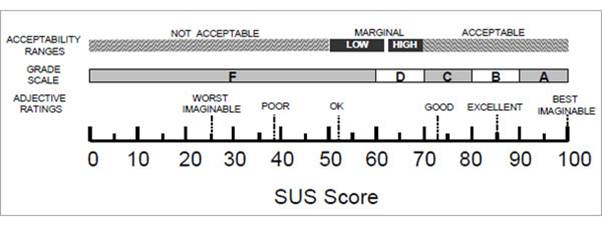
\includegraphics[width=0.95\textwidth]{images/SUS-Interpretation.jpg}
    \caption{Einstufung der SUS-Scores nach \citet{bangor_empirical_2008}}
    \label{fig:susInterpretation}
\end{figure}

\textbf{User Experience}

Neben der Usability ist auch die User Experience (UX) ein relevantes Konzept im Human Computer Interaction (HCI). Die DIN EN ISO 9241-210 definiert UX als \textit{„Wahrnehmungen und Reaktionen einer Person, die aus der tatsächlichen und/oder der erwarteten Benutzung eines Systems, eines Produkts oder einer Dienstleistung resultieren.“} \citep{DINISO9241}. Die UX ist demnach essentiell, um nachvollziehen zu können, wie ein interaktives Produkt oder System von Nutzenden wahrgenommen wird. Damit hat sie gleichzeitig einen erheblichen Einfluss auf den Erfolg eines Produktes oder Systems. Fallen die Reaktionen und Wahrnehmungen der Nutzenden negativ aus, wird sich dies auf den Erfolg des Produkts auswirken. Die Definition der DIN-Norm bietet, im Gegensatz zur Usability, jedoch keine Kriterien zur Messung. Um die UX messbar zu machen, wird das Modell der pragmatischen und hedonischen Qualität nach \citet{hassenzahl_user_2008} verwendet. Danach setzt sich die UX aus der pragmatischen und der hedonischen Qualität zusammen. Unter pragmatischer Qualität wird die aufgabenbezogene Qualität eines Produktes verstanden. Ein Produkt besitzt pragmatische Qualität, wenn es Nutzende dabei unterstützt, Aufgaben effizient und effektiv zu erledigen. Die hedonische Qualität hingegen bezieht sich auf nicht aufgabenbezogene Aspekte eines Produktes. Dazu zählen beispielsweise Aspekte wie Einzigartigkeit und Originalität. Viele etablierte Methoden zur Evaluation der UX basieren auf dieser Unterscheidung von Qualitäten. 

Die meisten Messmethoden der UX wurden für 2D-Anwendungen, wie Webseiten, Apps o. Ä. erstellt und validiert worden. Für VR-Anwendungen gibt es derzeit noch keine etablierten oder standardsierten Methoden zur Messung der UX \citep{alexandrovsky_evaluating_2021}. Am häufigsten werden jedoch quantitative Methoden zur Messung bei VR-Anwendungen eingesetzt \citep{kim_systematic_2020}. Ein häufig eingesetzter Fragebogen ist der User Experience Questionnaire (UEQ) \citep{laugwitz_construction_2008}. Dieser besteht aus 26 bipolaren Items und verwendet eine 7er Likert-Skala. Gemessen werden die UX-Faktoren Attraktivität, Druchschaubarkeit, Effizienz, Steuerbarkeit, Stimulation und Originalität. Der UEQ steht in über 20 Sprachen zur Verfügung. Der Fragebogen sowie ein spezifisches Auswertungstool kann kostenlos genutzt werden. 

\section{PaneoVR}

Das PaneoVR-Tool wurde entwickelt, um immersive 360°-Videotrainings bereitzustellen und die Erstellung virtueller Lehrinhalte für Bildungszwecke zu vereinfachen. Es handelt sich dabei um eine Web- und VR-Anwendung, die es Nutzenden ermöglicht, ohne tiefgehende Fachkenntnisse in Informatik oder Medientechnik ansprechende VR-Szenarien zu erstellen und zu nutzen \citep{noauthor_paneovr_nodate}. Das Konzept wurde im Rahmen des vom Bundesministerium für Bildung und Forschung geförderten Projekts ViRDiPA \citep{noauthor_virdipa-_nodate} entwickelt. Dieses Projekt lief vom 01.03.2020 bis zum 31.08.2023 und hatte das Ziel, VR als innovative Lehrmethode in der Pflegeausbildung zu etablieren. Die Entwicklung erfolgt in Zusammenarbeit mit dem Mixed Reality Lab der Hochschule Emden/Leer.

PaneoVR richtet sich an Personen, Unternehmen oder Einrichtungen, die eigenständig virtuelle Trainings ohne den Aufwand und die Kosten aufwendiger 3D-Designs und Animationen erstellen möchten. Stattdessen nutzt das Tool 360°-Videos, die eine realitätsgetreue Darstellung auf einfache Weise ermöglichen. Diese Methode erlaubt es, Szenarien von einfachen Raumtouren bis hin zu komplexen Rollenspiel-Erlebnissen zu erstellen. Nutzende stehen innerhalb von Video- oder Fotosphären und können durch Interaktion mit digitalen Elementen Einfluss auf die Umgebung nehmen, was eine dynamische und immersive Erfahrung schafft \citep{noauthor_paneovr_nodate}.

Das Tool besteht aus drei wesentlichen Komponenten:

\begin{itemize}
    \item \textbf{Diagrammeditor/Webeditor:}
    Der nodebasierte Diagrammeditor bildet die zentrale Plattform zur Erstellung der VR-Szenarien. Nutzende können 360°-Videos, Bilder und Audiodateien hochladen und daraus interaktive Szenen gestalten und zu Szenarien verknüfpen. 
    \item \textbf{VR-Anwendung/PaneoVR App:}
    Die PaneoVR App läuft auf allen gängigen VR-Brillen und ermöglicht es, die erstellten Szenarien direkt in Virtual Reality zu durchlaufen. Zusätzlich bietet die App einen Editor-Modus, über den unter anderem die Positionierung interaktiver Elemente in der Szene angepasst werden kann. 
    \item \textbf{Web Player:}
    Als Alternative zur VR-Anwendung erlaubt der Web Player, die Szenarien auf einem Rechner zu durchlaufen oder zu bearbeiten.
\end{itemize}

PaneoVR bietet eine Vielzahl interaktiver Elemente, die es Nutzenden ermöglichen, Szenarien individuell und ansprechend zu gestalten. Die Basisfelder repräsentieren dabei die einfachsten Interaktionsmöglichkeiten und dienen der einfachen Navigation zwischen Szenen innerhalb eines Szenarios. Zu den Basisfeldernzählen die Elemente \textit{Wegpunkt}, \textit{Benutzen} und \textit{Textpunkt}. Diese erlauben es, durch einen Klick zur jeweils verknüpften Szene zu wechseln. Die Elemente unterscheiden sich dabei nur in der Darstellung des Buttons und nicht in ihrer Funktionsweise. Auch \textit{automatische Wechsel} können integriert werden. Hierbei erfolgt der Szenenwechsel automatisch nach Abschluss des laufenden Szenenvideos. Dieses Element wird in der Szene nicht dargestellt. 
Für komplexere und nicht-lineare Szenenwechsel stehen Verzweigungselemente zur Verfügung. Das \textit{Dialog-Element} bietet bis zu vier verschiedene Multiple-Choice-Optionen, die beispielsweise als Antworten auf zuvor im Video gesagte Inhalte verwendet werden können. Jede Option kann mit einer nachfolgenden Szenen verknüpft und textlich dargestellt werden. Das \textit{Quiz-Element} ähnelt dem Dialog, beinhalet jedoch eine zentrale Frage, die in der Mitte der  Multiple-Choice-Antworten dargestellt wird. Das \textit{Zufällig-Element} wird in der Szene wie ein einfacher Wegpunkt dargestellt. Bei Auswahl dieses Elements wird jedoch zufällig eine der verknüpften Szenen ausgewählt, was eine dynamische Variation innerhalb eines Szenarios erlaubt.
PaneoVR bietet außerdem die Möglichekit, Bilder in die Szenen einzubinden und diese interaktiv zu nutzen. Ein \textit{Bild-Element} bindet das gewählte Bild als Miniaturansicht in die Szene ein. Wird dieses ausgewählt, erscheint eine vergrößerte Ansicht des Bildes, die über einen Zurück-Button wieder geschlossen werden kann. Das Element \textit{Untersuchen} verfolgt einen ähnlichen Ansatz, ersetzt jedoch die Miniaturansicht durch einen Button mit dem Icon einer Lupe, um den Eindruck eines detaillierten Betrachtens zu vermitteln. Der \text{Bild-Wegpunkt} verbindet die Anzeige eines Miniaturbilds mit der Funktionsweise eines Wegpunkts. Wird das Element ausgewählt, erfolgt ein Szenenwechsel. 
Auditive Elemente spielen ebenfalls eine zentrale Rolle bei der Gestaltung immersiver Szenarien. Hintergrundsounds wie Musik, Umgebungsgeräusche oder nachträglich synchronisierte Inhalte können über das \textit{Audio-Element} einer Szene hinzugefügt werden. Diese werden automatisch beim Start einer Szene abgespielt. Das Element \textit{Audio-Anwählbar} erlaubt es den Nutzenden, Audiodateien gezielt durch Klicken eines Play-Buttons zu starten. Über einen \textit{Audio-Wegpunkt} kann ein automatischer Szenenwechel nach Beendigung der abgespielten Audiodatei integriert werden. 
Darüber hinaus gibt es das Element \textit{Hinweis}, welches nach einer definierten Zeitspanne einen eingeblendeten Text als Pop-up erscheinen lässt. Dies kann genutzt werden, um zusätzliche Informationen oder Hilfestellungen zu vermitteln. Schließlich können Szenarien durch \textit{Szenario-Ende-Elemente} abgeschlossen werden. \textit{Szenario Abgeschlossen} färbt die Szene grün und signalisiert den erfolgreichen Abschluss, während \textit{Szenario Fehlgeschlagen} eine rote Markierung verwendet, um ein Scheitern anzuzeigen. Auch bei diesen Elementen öffnet sich ein Pop-Up, über das das Szenario beendet oder fortgesetzt werden kann.

Die vorliegende Arbeit basiert auf der PaneoVR-App für VR-Brillen. Der Schwerpunkt liegt auf der Integration binärer Interaktionsschnittstellen, um die Nutzung der erstellten Szenarien zu verbessern. Der Editor-Modus der App wird dabei bewusst vernachlässigt, da der Fokus auf dem Durchlaufen und der Interaktion mit den Szenarien liegt.

\section{Zusammenfassung} 

In diesem Kapitel wurden die theoretischen und technologischen Grundlagen sowie der aktuelle Forschungsstand dargelegt, um die Relevanz dieser Arbeit zu unterstreichen und eine Grundlage für Entscheidungen zu schaffen, die im Rahmen der Konzeption sowie der Planung der Evaluation getroffen werden. Darüber hinaus bilden sie die Grundlage für die Einordnung der in der Evaluation erhobenen Ergebnisse.

Es wurde dargelegt, dass der Forschungsbereich der Barrierefreiheit in VR ein relativ junges Forschungsfeld ist, das erst in den vergangenen Jahren vermehrt an Aufmerksamkeit gewonnen hat. Es existieren bisher nur wenige Richtlinien für die Entwicklung von barrierearmen VR-Anwendungen, an denen sich Entwickler:innen orientieren können. Aus der Übersicht und Zusammenfassung von Richtlinien von \citet{heilemann_accessibility_2021} wird in Bezug auf die Kategorien Steuerung und Eingabe deutlich, dass eine Notwendigkeit vorliegt, einfache Steuerungsschemata bereitzustellen sowie assistive Technologien wie Schalter in VR-Anwendungen zu integrieren. Diese Notwendigkeit konnte im weiteren Verlauf des Kapitels durch die Analyse bestehender Barrieren für Menschen mit motorischen Beeinträchtigungen bestätigt werden. Es wurde aufgezeigt, dass aktuelle VR-Systeme primär für nicht-behinderte Personen ausgelegt sind \citep{wong_survey_2017}  und viele verbreitete Nutzungsanforderungen, wie die Bedienung von Controllern oder die Durchführung präziser Bewegungen zur Interaktion, Menschen mit motorischen Beeinträchtigungen von der Nutzung dieser Systeme ausschließen \citep{dombrowski_designing_2019}. Obwohl bereits einige theoretische Lösungsansätze zur Überwindung dieser Barrieren existieren, gibt es bisher nur wenige Arbeiten, in denen praktische Implementierungen hinsichtlich alternativer Interaktionsmethoden durchgeführt wurden. Als Alternative zur klassischen Point-and-Select-Interaktion mittels VR-Controller haben bspw. \citet{valakou_framework_2024} eine Interaktionsmethode mittels sequentiellen Scanning in ihr entwickeltes XR Accessibility Framework integriert. Eine ausführliche Testung und Evaluation dieses Frameworks steht jedoch noch aus. Auch die von \citet{creed_inclusive_2024_2} entwickelte Forschungsagenda zur Barrierefreiheit in VR hebt die Notwendigkeit hervor, alternative Eingabemethoden zu entwickeln und Systeme zu schaffen, die mit bestehenden assistiven Technologien kompatibel sind.
Diese Ergebnisse betonen die Relevanz der vorliegenden Arbeit und weisen auf einen deutlichen Bedarf in der Entwicklung und Untersuchung alternativer Interaktionsschnittstellen hin, um Menschen mit motorischen Beeinträchtigungen die Nutzung von VR-Anwendungen zu erleichtern bzw. zu ermöglichen. Binäre Interaktionsschnittstellen stellen in diesem Zusammenhang eine vielversprechende Lösung dar, da sie Interaktionen ohne präzise Bewegungen oder umfangreiche motorische Fähigkeiten ermöglichen und die Einbindung von Schaltern als assistive Technologie erlauben. Die große Vielfalt an verfügbaren Schaltern ermöglicht eine flexible Anpassung an die individuellen Bedürfnisse der Nutzenden. 

Um im Rahmen der Konzeption fundierte Gestaltungsentscheidungen treffen zu können, wurden in diesem Kapitel gängige Scanning-Verfahren hinsichtlich ihrer Vor- und Nachteile präsentiert. Darüber hinaus wurde eine Einführung in den theoretischen Hintergrund von VR als Technologie gegeben, bei der Immersion, Interaktivität und Presence zentrale Konzepte dargestellt wurden. Des Weiteren wurde das Auftreten von Motion Sickness als Herausforderung bei der Nutzung von VR-Anwendungen genauer betrachtet. In ihrer Zusammenfassung von Richtlinien betonen \citet{heilemann_accessibility_2021}, dass VR-spezifische Trigger für Motion Sickness in der Entwicklung von Anwendungen möglichst zu vermeiden sind. Dies sollte demnach bei der Konzeption der Interaktionsschnittstellen berücksichtigt werden. Darüber hinaus wurde auf die Bedeutung von Usability und UX als Evaluierungsinstrumente für VR-Anwendungen eingegangen. Die etablierten Methoden, wie die SUS und der UEQ, ermöglichen eine einfache und schnelle Evaluierung dieser Konzepte. Der vorliegende theoretische Hintergrund verdeutlicht somit, dass im Rahmen der späteren Evaluation der konzipierten und implementierten Interaktionsschnittstellen insbesondere die Konzepte der Usability, UX sowie des Auftretens von Motion Sickness berücksichtigt und untersucht werden sollten. Die vorgestellten Informationen zur Interpretation der SUS von \citet{bangor_empirical_2008}, das ausführliche Auswertungstool für den UEQ und die Informationen zur Interpretation der Ergebnisse des SSQ nach \citet{stanney_cybersickness_1997} liefern dabei eine wertvolle Grundlage, um die im Rahmen der Evaluation erhobenen Daten einzuordnen. 

Die gewonnenen Erkenntnisse aus diesem Kapitel bilden eine umfassende Grundlage für die im Folgenden vorgestellte Konzeption. Aufbauend auf den identifizierten Forschungslücken, bestehenden Barrieren und theoretischen Grundlagen werden im nächsten Kapitel die methodischen und technischen Überlegungen zur Gestaltung binärer Interaktionsschnittstellen für VR-Anwendungen dargelegt.
\chapter{Konzeption}
\label{chap:Konzept}

%To DOs für dieses Kapitel: Tabellen überarbeiten, Texte überarbeiten/anpassen, Kapiteleinleitungen und fehlende Abschnitte schreiben, Quellen einfügen (vgl. Kommentare Overleaf), Bezug zu FF1 herstellen

In diesem Kapitel wird die Konzeption der beiden binären Interaktionsschnittstellen dargelegt. Diese Konzeption bildet das Fundament dieser Arbeit, da sie die Grundlage für die spätere Implementierung und Evaluation legt. Der Prozess folgt einem systematischen Ablauf, der auf den Grundprinzipien der morphologischen Analyse von \citet{10.1007/978-3-642-87617-2_14} basiert und für den spezifischen Kontext dieser Arbeit angepasst wurde. Diese Methode ermöglicht eine strukturierte und umfassende Betrachtung des Design Space. Der Ablauf besteht aus vier zentralen Schritten:

\begin{itemize}
    \item \textbf{Definition des Design Space:}
    In diesem Schritt werden die grundlegenden Gestaltungsmöglichkeiten und Anforderungen für die Interaktionen erarbeitet. Dazu werden die für die Zielsetzung dieser Arbeit relevanten Interaktionsaufgaben abgeleitet sowie Interaktionskomponenten und -Parameter identifiziert.
    \item \textbf{Erarbeitung konkreter Ausprägungen:}
    Auf Grundlage des definierten Design Space werden spezifische Ausprägungen für die Interaktionsaufgaben und -komponenten entwickelt, die die Bandbreite möglicher Ansätze abbilden.
    \item \textbf{Einordnung anhand der Parameter:}
    Die erarbeiteten Optionen werden systematisch anhand der zuvor identifizierten Parameter eingeordnet. Dieser Schritt dient dazu, die Designentscheidungen transparent darzulegen und zu begründen.
    \item \textbf{Ableitung der finalen Konzepte:}
    Abschließend werden die finalen Konzepte für die beiden binären Interaktionsschnittstellen abgeleitet, die anschließend im Prototyp implementiert werden.
\end{itemize}
 
Durch diese strukturierte Vorgehensweise wird die erste Forschungsfrage (FF1) adressiert.   

\section{Definition des Design Space}

Die Beschreibung des Design Space für binäre Interaktionen in PaneoVR basiert auf einer hierarchischen Struktur mit drei Ebenen. Die grundlegende Ebene wird durch die Interaktionsaufgaben definiert, die die für die Nutzung der Anwendung erforderlichen Interaktionsarten umfassen. Die zweite Ebene umfasst die Interaktionskomponenten, die spezifische Teilaspekte der Interaktion näher bestimmen. Die letzte Ebene bilden die Parameter. Parameter beschreiben in diesem Kontext Designüberlegungen, anhand derer die Interaktionstechniken und -ausprägungen bewertet werden. Die definierten Parameter beeinflussen dabei das gesamte VR-Erlebnis \citep{10.1145/3441852.3471230}. Die Kombination verschiedener Ausprägungen von Interaktionsaufgaben und -komponenten aus diesem Design Space kann anschließend als Grundlage für die Entwicklung neuartiger Interaktionstechniken verwendet werden.

{\normalfont \bfseries Interaktionsaufgaben:}  

Die Nutzung der mit PaneoVR erstellten Trainings basiert auf zwei grundlegenden Interaktionsaufgaben. Die erste Interaktionsaufgabe besteht in der Selektion von Interaktionselementen innerhalb der Szene, d.h. von Elementen wie z. B.  Wegpunkten oder Dialogfeldern, sowie von UI-Elementen, z. B. innerhalb des Hauptmenüs. Die zweite Interaktionsaufgabe umfasst die Navigation innerhalb der Szene. Dies umfasst die Änderung der Blickrichtung innerhalb der Szene. Da PaneoVR keinen dreidimensionalen Navigationsraum bereitstellt, sondern lediglich 360°-Videos präsentiert, ist eine klassische Navigation im 3D-Raum nicht notwendig. Stattdessen genügt eine Rotation der Szene, um die Blickrichtung zu ändern und damit innerhalb der virtuellen Welt zu navigieren. Da davon auszugehen ist, dass Nutzende mit motorischen Beeinträchtigungen Kopfbewegungen nicht frei und ohne Einschränkungen ausführen können, ist die Entwicklung einer alternativen Navigationsform unabdingbar. 

{\normalfont \bfseries Interaktionskomponenten:} 
%Überlegung: Ist Fehlerkorrektur eine Komponente? 

In Bezug auf die Interaktionen in PaneoVR lassen sich insgesamt drei verschiedene Komponenten identifizieren, deren konkrete Ausgestaltung einen direkten Einfluss auf die Erfahrung nimmt. 

Die Komponente Display definiert Darstellung und Integration des Interaktionsverfahren in die virtuelle Umgebung. Im Rahmen der Festlegung der Interaktionskomponente ist insbesondere zu bestimmen, ob sich die Interaktion auf das Sichtfeld des Nutzenden beschränkt. Die Relevanz dieser Komponente zeigt sich insbesondere in Kontexten, in denen Nutzende in der Lage sind, ihren Kopf zu bewegen und damit ihr Blickfeld unabhängig von der binären Interaktionsschnittstelle zu verschieben.

Eine weitere zu berücksichtigende Komponente ist die Transition. Diese ist insbesondere bei der Betrachtung des Navigationsprozesses von Bedeutung. Die Transition beschreibt die Art und Weise, wie die Drehung der First-Person-Kamera erfolgt, wenn Nutzende eine navigationsbezogene Interaktion durchführen. Das heißt, Transition beschreibt den Übergang zwischen der aktuellen und der neuen Blickrichtung.

Die letzte relevante Komponente ist die Initialisierung. Dabei wird festgelegt, ob das gewählte Interaktionsverfahren automatisch und kontinuierlich aktiv ist oder zunächst durch eine initiale Interaktion initialisiert werden muss. 

{\normalfont \bfseries Parameter:} 

Die Entwicklung und Bewertung von Interaktionen basiert in der Regel auf der Berücksichtigung verschiedener Parameter, welche das Gesamterlebnis einer VR-Anwendung maßgeblich beeinflussen \citep{10.1145/3441852.3471230}. Die relevanten Parameter für die Interaktionen in PaneoVR werden auf Basis vorangegangener Forschungsarbeiten identifiziert. Da die Gewährleistung einer guten Usability das primäre Ziel der Gestaltung von Interaktionen in VR darstellt \citep{dorner_virtual_2019}, werden die Parameter Effizienz \citep{DINISO9241-11}, Effektivität \citep{DINISO9241-11}, Erlernbarkeit \citep{DINISO9241-110} sowie Robustheit \citep{DINISO9241-110} definiert. Darüber hinaus werden die Parameter Interaktionsgeschwindigkeit \citep{COOK2015117} und Komfort \citep{jerald_vr_2016} berücksichtigt. 

\textit{Effizienz} beschreibt das Verhältnis zwischen den eingesetzten Ressourcen und dem damit erreichten Ziel \citep{DINISO9241-11}. Im Anwendungskontext ist  insbesondere der benötigte Aufwand als relevante Ressource zu betrachten.

\textit{Effektivität} bezeichnet die Genauigkeit und Vollständigkeit, mit der Benutzer ihre Ziele erreichen. Sie beschreibt, inwieweit die tatsächlichen Ergebnisse mit den angestrebten übereinstimmen. Je nach Kontext kann die Genauigkeit entweder anhand der Korrektheit eines Ergebnisses oder anhand des Erreichens eines akzeptablen Grads der Übereinstimmung mit dem Ziel bewertet werden \citep{DINISO9241-11}.

\textit{Erlernbarkeit} beschreibt das Ausmaß, in dem eine Interaktion ohne vorherige Einarbeitung verstanden und genutzt werden kann. In diesem Kontext ist von Relevanz, dass insbesondere ein hoher Wiedererkennungswert der Interaktion eine einfache und intuitive Bedienbarkeit bedingt \citep{jerald_vr_2016}.

\textit{Robustheit} beschreibt die Fähigkeit eines Systems, auf Fehler von Nutzenden angemessen zu reagieren \citep{DINISO9241-110}. Im Rahmen dieser Betrachtung wird untersucht, welche Maßnahmen ergriffen werden, um das Auftreten von Fehlern zu verhindern und inwiefern eine Korrektur von Fehlern möglich ist.

\textit{Interaktionsgeschwindigkeit} beschreibt die Zeit, die benötigt wird, um ein Interaktionsziel zu erreichen. Es wird somit die Zeit betrachtet, die für die Ausführung einer Interaktionsaufgabe benötigt wird. Im Rahmen dieser Betrachtung wird insbesondere die Wartezeit während der Interaktion analysiert.  

\textit{Komfort} bezeichnet die Wahrnehmung der Nutzenden bezüglich der Angenehmheit der Interaktion \citep{jerald_vr_2016}. In diesem Zusammenhang ist insbesondere die Wahrscheinlichkeit des Auftretens von Motion Sickness von Bedeutung. Dabei werden Faktoren wie Ermüdung, erhöhte Konzentration und visuelle Komplexität in die Bewertung einbezogen.

\section{Ausprägungen der Interaktionsaufgaben und Komponenten}

Folgend werden mögliche Ausprägungen zur Implementierung der zuvor beschriebenen Interaktionsaufgaben und Komponetnen erörtert.

{\normalfont \bfseries Interaktionsaufgaben}  

1. Selektion: 

Die Realisierung einer binären Interaktion erfordert die Implementierung einer indirekten Selektionsmethode. In diesem Zusammenhang sind Scanning-Verfahren eine der am weitesten verbreiteten Methoden \citep{COOK2015117}. Zur Implemntierung in PaneoVR werden die gängigen Scanning-Verfahren Automatic Item Scanning, Step Item Scanning mit Dwell Selection, Inverse Item Scanning sowie Continueous Cartesian Scanning (vgl. \autoref{subchap:Scanning}) in Betracht gezogen. 

2. Navigation:

Im Sinne einer konsistenten Gestaltung sollte die Art der Interaktion bei der Navigation einheitlich zu der bei der Selektion sein. Damit soll erreicht werden, dass sich das System für die Nutzenden möglichst erwartungskonform verhält. In dieser Konsequenz bedingt sich die Auswahl der Ausprägungen gegenseitig.

In der Literatur liegen bisher keine konkreten Umsetzungen für binäre Navigationsschnittstellen in VR vor. Ein Ansatz, den bspw. \citet{wentzel_bring-your-own_2023} beschreibt, wäre die Übertragung von bereits existierenden Accessibility-Techniken für Smartphones auf den Einsatz in VR. Eine weit verbreitete Technik bei Smartphones besteht darin, dass sich ein Cursor von links nach rechts über den Bildschirm bewegt und der Nutzende durch das Drücken eines Schalters an die gewählte Position teleportiert wird \citep{wentzel_bring-your-own_2023}. Dieses Prinzip lässt sich auf das Continuous Cartesian Scanning übertragen. Anstelle eines Cursors wird hier der gesetzte Schnittpunkt der Scan-Linien als Zielpunkt der Navigation gewählt. Im Kontext dieser Arbeit, in dem die Navigation lediglich aus einer Rotation der First-Person-Kamera besteht, würde dies konkret bedeuten, dass zunächst der Schnittpunkt gesetzt wird und die Kamera daraufhin so rotiert wird, dass der Mittelpunkt des Blickfelds auf den definierten Schnittpunkt ausgerichtet wird. 

Aus diesem Grundprinzip lassen sich zwei konkrete Optionen für die Navigation ableiten.

\begin{itemize}
    \item Direkte Navigation: Hier werden Navigation und Selektion in einem Prozess kombiniert. Sobald der Schnittpunkt der Scan-Linien gesetzt ist, prüft das System, ob sich an diesem Punkt ein interaktives Element befindet. Ist dies der Fall, wird das entsprechende Element selektiert. Ist kein interaktives Element vorhanden, wird stattdessen die Kamera auf die Position des Schnittpunktes ausgerichtet und die Navigation durchgeführt.
    \item Navigations- und Selektionsmodus: Es stehen zwei getrennt nutzbare Modi zur Verfügung, ein Navigationsmodus und ein Selektionsmodus. Im Navigationsmodus führt das Setzen eines Schnittpunktes immer zu einer Navigation, unabhängig davon, ob sich hinter dem Schnittpunkt ein interaktives Element befindet oder nicht. Im Selektionsmodus hingegen wird der Schnittpunkt ausschließlich zur Selektion von Interaktionselementen verwendet. Befindet sich kein interaktives Element hinter dem Schnittpunkt, wird keine Aktion ausgeführt. Diese klare Trennung der Modi stellt sicher, dass im Navigationsmodus keine Selektion und im Selektionsmodus keine Navigation möglich ist.
\end{itemize}

Auch in Bezug auf das Item Scanning können bereits existierende Accessibility-Techniken als Inspiration für die Entwicklung einer Navigation in VR herangezogen werden. In Computerspielen ist es z. B. möglich, Steuerungen durch Buttons auf dem Bildschirm darzustellen und so für die Auswahl durch Scanning zugänglich zu machen (vgl. z. B. \citep{10.1145/2159365.2159386, trewin_exploring_2009}).  
Dieses Prinzip könnte auch auf VR-Anwendungen übertragen werden. Hier könnten Buttons für die Rotationsrichtungen (links und rechts) in ein UI-Navigationsmenü integriert werden.  Hinsichtlich der genauen Funktionsweise der Buttons können wiederum zwei mögliche Ausprägungen unterschieden werden. 

\begin{itemize}
    \item Diskrete Rotation: Die Selektion eines Buttons bewirkt eine Rotation um einen festen Winkel. Um eine größere Rotation zu erreichen, muss der entsprechende Button wiederholt selektiert werden.
    \item Kontinuierliche Rotation: Die Selektion eines Buttons löst eine kontinuierliche Rotation in die vom Nutzenden gewählte Richtung aus. Durch erneute Selektion des entsprechenden Buttons kann die Rotation jederzeit gestoppt werden. Ein vergleichbares Prinzip wurde z. B. von \citet{10.1145/2159365.2159386} zur Navigation von Spielavataren entwickelt und evaluiert. 
\end{itemize}

{\normalfont \bfseries Interaktionskomponenten}  

1. Display:

Die Interaktionskomponente \textit{Display} bezieht sich auf die Darstellung und Integration des Scanning-Verfahrens in die virtuelle Umgebung. Dabei ist insbesondere entscheidend, ob sich das Scanning-Verfahren auf das Sichtfeld der Nutzenden beschränkt oder die gesamte 360°-Szene einbezieht. Da es sich somit um eine VR-spezifische Komponente handelt, können diesbezüglich keine Ansätze aus anderen Bereichen wie Computerspielen oder Smartphones als Grundlage herangezogen werden. Wie bereits in \autoref{subchap:LösungenFürBarrieren} dargestellt, gibt es in der Literatur kaum Arbeiten, die sich speziell mit der Integration von binären Eingaben oder Scanning-Verfahren in VR auseinandersetzen. Eine Ausnahme bildet die Arbeit von \citet{valakou_framework_2024}, in der jedoch keine konkreten Aussagen zur Gestaltung der Interaktionskomponente Display getroffen werden. Aus diesen Gründen basieren die folgenden Überlegungen nicht auf bestehenden Forschungsarbeiten, sondern stellen eigenständige Konzepte dar.

Für die Gestaltung der Komponente \textit{Display} wurden zwei grundlegende Optionen entwickelt.

\begin{itemize}
    \item Fixiert im Sichtfeld: Das Scanning-Verfahren ist wie ein Head-Up-Display (HUD) im Sichtfeld des Nutzers fixiert. Das bedeutet, dass das Verfahren an die Blickrichtung des Nutzenden gekoppelt ist, sodass nur Elemente ausgewählt werden können, die sich innerhalb des Sichtfeldes befinden. Dies ermöglicht es, beim Cartesian Scanning die Position der Scan-Linien durch Kopfbewegungen direkt zu beeinflussen. Beim Item Scanning wirken sich Kopfbewegungen ebenfalls auf das Scanning aus, da hier das Scan-Set dynamisch angepasst wird. Elemente, die durch eine Kopfbewegung aus dem Sichtfeld verschwinden, werden aus dem Scan-Set entfernt, wodurch sich dessen Größe dynamisch verändert.
    \item 360°-Szene: Der Scanning-Verfahren ist ein integraler Bestandteil der Szene. Das Scanning kann daher nicht durch Kopfbewegungen beeinflusst werden. Beim Cartesian Scanning bewegen sich die Scanlinien unabhängig von der Blickrichtung in einem Radius von 360° um den Nutzenden. Beim Item Scanning werden alle Interaktionselemente der Szene, auch außerhalb des Sichtfeldes, einbezogen und hervorgehoben. 
\end{itemize}

2. Transition: 

Die Rotation der Kamera bei der Navigation kann auf verschiedene Arten realisiert werden. In der Literatur (vgl. z. B. \citet{10.1145/3441852.3471230, 10.1007/s10055-020-00425-x, 8797722}) werden insbesondere die beiden folgenden Varianten diskutiert.

\begin{itemize}
    \item Direkte Rotation: Bei der direkten Rotation erfolgt eine unmittelbare Rotation der Kamera um einen vorgegebenen Winkel ohne intermediäre Schritte. 
    \item Kontinuierliche Rotation: Die zweite Option umfasst eine kontinuierliche Bewegung der Kamera. In diesem Fall erfolgt eine fließende Drehung der Szene um den Nutzenden, wodurch eine natürliche Kopfbewegung simuliert wird. 
\end{itemize}

3. Initialisierung 

Die Komponente \textit{Initialisierung} beschreibt, wie das Scanning Verfahren aktiviert wird und ob die Aktivierung durch die Nutzenden gesteuert werden kann. Dabei sind zwei Möglichkeiten denkbar. 

\begin{itemize}
    \item Automatisch: Das Scanning-Verfahren wird automatisch aktiviert und lässt sich auch nicht durch den Nutzenden deaktivieren. Das Verfahren läuft kontinuierlich durch die Szene sowie die gesamte Anwendung hindurch.
    \item Manuell: Das Scanning-Verfahren muss durch eine initiale Eingabe manuell aktiviert werden. 
\end{itemize}

{\normalfont \bfseries Zusammenfassung}

Die erarbeiteten Ausprägungen der Interaktionsaufgaben und -komponenten werden zusammenfassend in der \autoref{fig:MorphKasten-Leer} dargestellt. 

\begin{figure}[tbh]
    \centering
    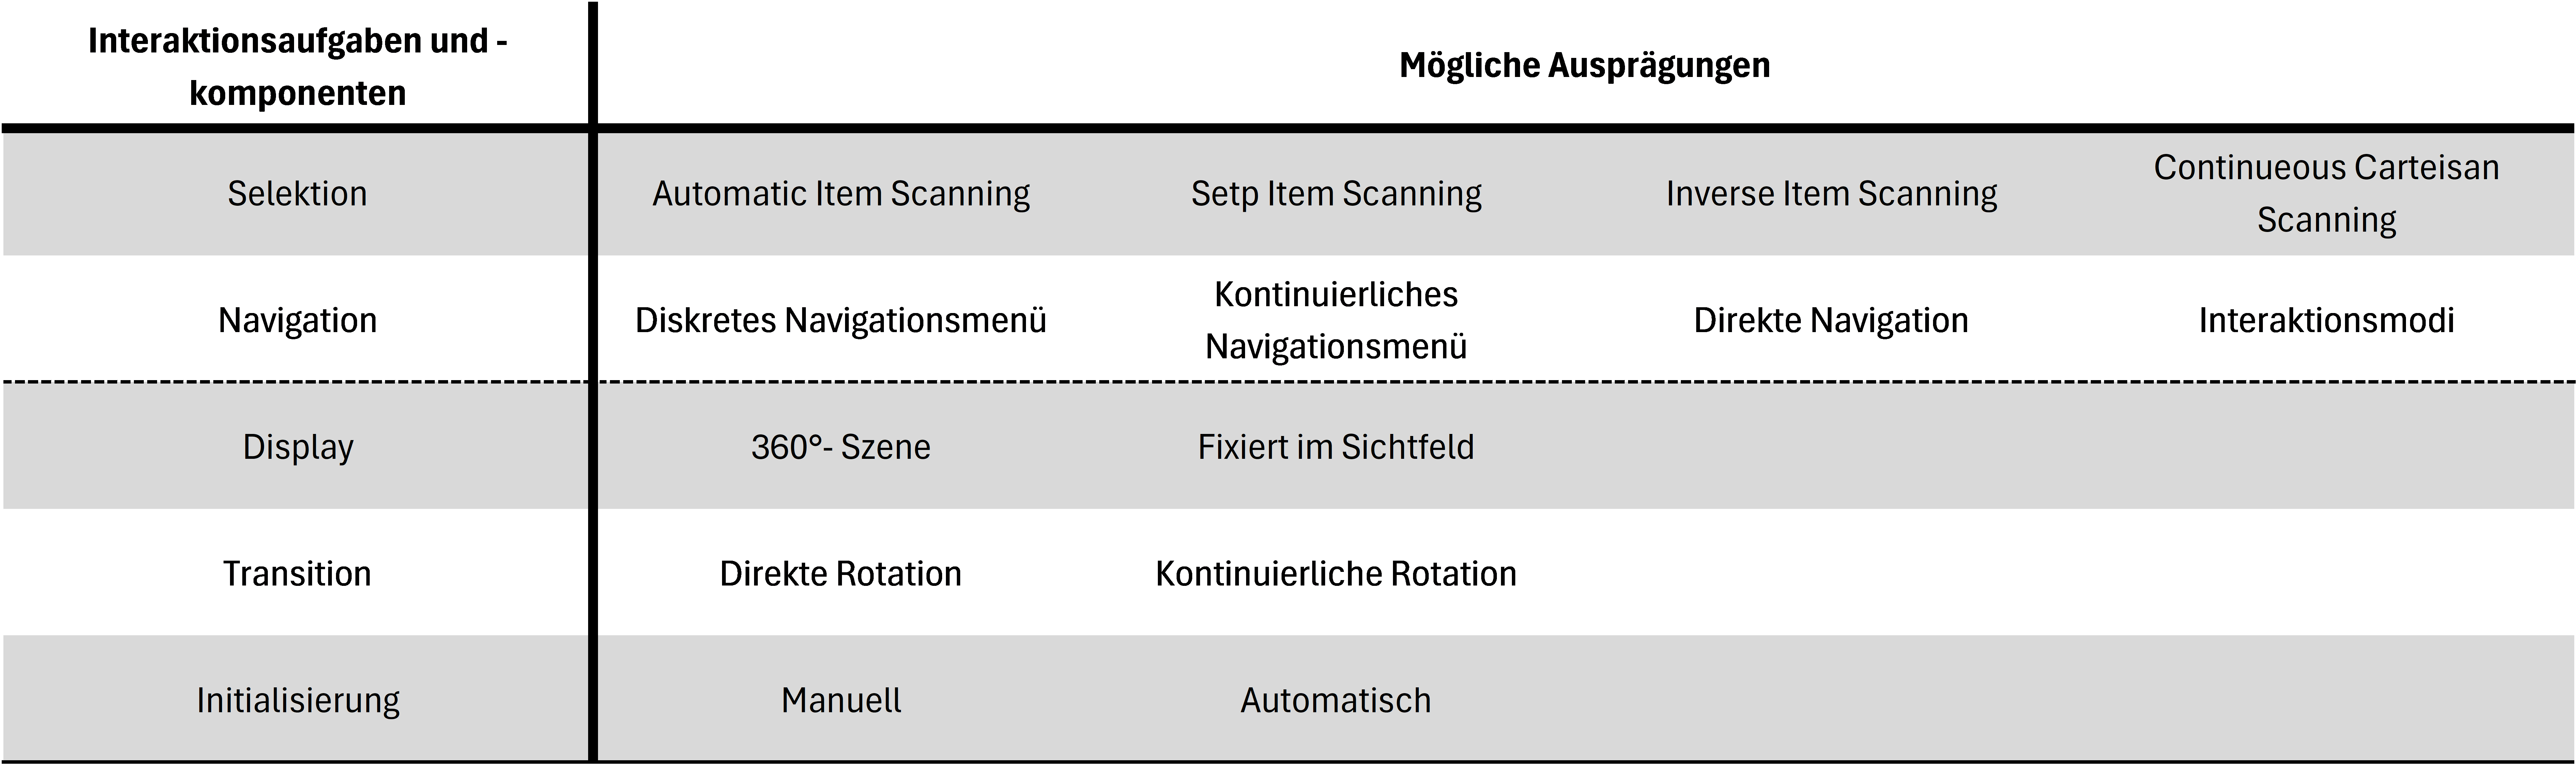
\includegraphics[width=0.95\textwidth]{images/MorphKasten-Ausgang.png}
    \caption{Darstellung der möglichen Ausprägungen der Interaktionsaufgaben und -komponenten}
    \label{fig:MorphKasten-Leer}
\end{figure}

\section{Einordnung und Bewertung der Interaktionsaufgaben und Komponenten anhand der Parameter}
\label{subchap:EinordnungNachParameter}

In diesem Abschnitt werden die zuvor beschriebenen Gestaltungsoptionen der Interaktionsaufgaben und -komponenten systematisch anhand der definierten Parameter bewertet und eingeordnet. Durch soll eine fundierte Grundlage für die Auswahl der finalen Konzepte geschaffen werden. Diese Einschätzung basiert auf den Erkenntnissen der Literatur sowie einer Analyse der vorgestellten Optionen. Es ist jedoch wichtig zu betonen, dass nicht alle Bewertungen durch empirische Daten belegt oder validiert sind, sondern auf einer fundierten, jedoch subjektiven Einschätzung beruhen. 

{\normalfont \bfseries Interaktionsaufgaben}  

\textbf{1. Selektion}

Im Folgenden erfolgt die Einordnung der für die Selektion erarbeiteten Gestaltungsoptionen anhand der definierten Parameter. Dabei wird jeder Parameter einzeln betrachtet, um die spezifischen Stärken und Schwächen der Optionen detailliert zu analysieren. Die Ergebnisse werden in \autoref{fig:Netz-Selektion} visualisiert und bieten eine zusammenfassende Darstellung der Parameterbewertungen.

\begin{figure}[tbh]
    \centering
    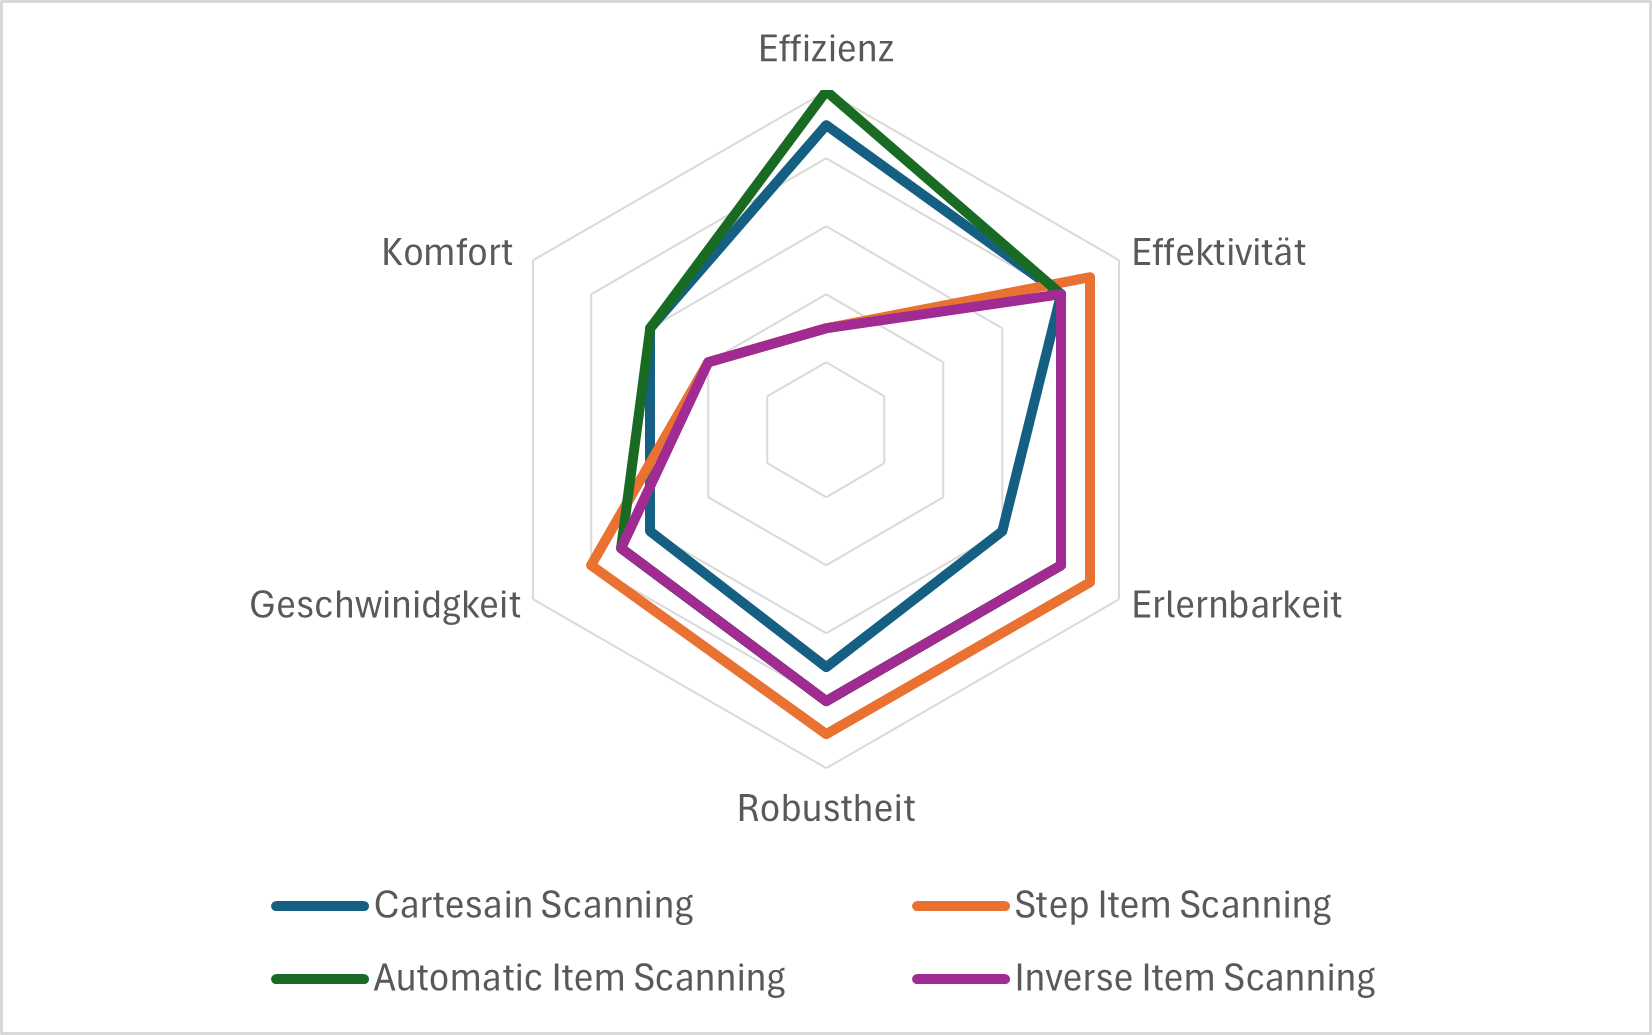
\includegraphics[width=0.75\textwidth]{images/Netzdiagramm-Selektion.png}
    \caption{Visualisierung der Einordnung der Gestaltungsoptionen der Interaktionsaufgabe Selektion}
    \label{fig:Netz-Selektion}
\end{figure}

\textit{Effizienz:}
Ein effizientes binäres Selektionsverfahren sollte eine geringe Anzahl von Schalterbetätigungen und einen möglichst geringen physischen Aufwand für die Interaktion erfordern. Die verschiedenen Auswahlverfahren unterscheiden sich in dieser Hinsicht deutlich. Cartesian Scanning erfordert zwei Schalteraktivierungen, um eine Interaktion durchzuführen. Die klare Struktur und die relativ geringe Anzahl an Aktivierungen ermöglichen eine gute Effizienz.. Automatic Item Scanning zeichnet sich durch eine besonders geringe Anzahl von Aktivierungen aus, da die Selektion eines Elements in der Regel durch eine einzige Schalteraktivierung erfolgt. Dies macht die Methode besonders effizient. Wird allerdings eine Gruppierung von Elementen zur Beschleunigung der Interaktionsgeschwindigkeit eingesetzt, wirkt sich dies leicht negativ auf die Effizienz aus, da die Anzahl der erforderlichen Aktivierungen steigt. Step Item Scanning zeigt eine Effizienz, die stark von der Anzahl der Elemente in der Szene abhängt. Bei einer großen Anzahl von Elementen benötigt das Verfahren entsprechend viele Aktivierungen, um ein Ziel zu erreichen, was die Effizienz deutlich verringert. Eine Gruppierung der Elemente kann jedoch die Effizienz in Szenen mit vielen Elementen erhöhen, da weniger Schritte notwendig sind, um eine Auswahl zu treffen. Auch in Szenarien mit wenigen Elementen ist der Aufwand höher als bei Cartesian Scanning oder Automatic Item Scanning. Inverse Item Scanning ist ebenfalls stark von der Anzahl der Elemente in der Szene abhängig. Je mehr Elemente vorhanden sind, desto länger muss der Schalter gehalten werden, um das gewünschte Zielobjekt zu erreichen. Dies führt zu einem proportionalen Anstieg der körperlichen Anstrengung und verringert die Effizienz in Szenen mit vielen Elementen. Bei wenigen Elementen ist der Aufwand entsprechend geringer. Dennoch bleibt das kontinuierliche Halten des Schalters eine körperlich anstrengendere Interaktionsform. 

\textit{Effektivität:}
Die Effektivität beschreibt, wie zuverlässig und präzise ein gewünschtes Interaktionselement ausgewählt werden kann. Das Cartesian Scanning erfordert präzises Timing, da der Nutzende den Schnittpunkt der Linien im richtigen Moment setzen muss. Ein Verfehlen des Zielobjekts ist möglich, insbesondere bei geringer Übung oder hohen Geschwindigkeiten des Scannings. Das Cartesian Scanning ermöglicht jedoch eine sehr präzise Selektion, insbesondere mit etwas Erfahrung. 
Das Automatic Item Scanning erzielt eine leicht höhere Effektivität. Da nur interaktive Elemente selektiert werden können, sind Fehlselektionen weniger wahrscheinlich. Dennoch spielt auch hier das Timing eine wesentliche Rolle, da das gewünschte Element verpasst werden kann, wenn die Aktivierung nicht rechtzeitig erfolgt. Das Step Item Scanning wird als das effektivste Verfahren eingeschätzt. Die Nutzenden haben die volle Kontrolle über die Auswahl und können in ihrem eigenen Tempo navigieren. Dies minimiert die Wahrscheinlichkeit von Fehlselektionen und gibt ihnen mehr Sicherheit, insbesondere in komplexen Szenarien mit vielen Elementen. Das Inverse Item Scanning zeigt eine Effektivität, die mit der des Automatic Item Scannings vergleichbar ist. Auch hier ist das Timing entscheidend, da der Schalter zum richtigen Zeitpunkt losgelassen werden muss, um das gewünschte Ziel zu erreichen. Die Möglichkeit von Fehlselektionen durch ungenaues Timing ist ein potenzieller Nachteil \citep{COOK2015117}.

\textit{Erlernbarkeit:}
Die Erlernbarkeit beschreibt, wie schnell und intuitiv ein Scanning-Verfahren von den Nutzenden verstanden und angewendet werden kann. Das Step Item Scanning weist die höchste Erlernbarkeit auf. Es ermöglicht den Nutzenden die größte Kontrolle über das Scanning, da sie in ihrem eigenen Tempo navigieren können. Diese direkte Steuerbarkeit reduziert die kognitiven und sensorischen Anforderungen \citep{cook_chapter_2015}, was sich positiv auf das Verständnis der Funktionsweise auswirken könnte. Automatic Item Scanning und Inverse Item Scanning sind in ihrer Erlernbarkeit vergleichbar. Beide Verfahren erfordern die Fähigkeit, das richtige Timing zu finden, um das gewünschte Element auszuwählen. Cartesian Scanning wird als das herausforderndste Verfahren eingestuft. Hier müssen die Nutzenden sowohl der horizontalen als auch der vertikalen Bewegung der Scan-Linien folgen, was ein höheres Maß an Aufmerksamkeit erfordert. Darüber hinaus sind genauere Eingaben erforderlich. Insbesondere für Personen, die mit Scanning-Verfahren weniger vertraut sind, könnte dies anfangs zu Schwierigkeiten führen.
Insgesamt dürften Personen mit Vorerfahrung im Umgang mit Schaltersteuerungen alle beschriebenen Verfahren als vertraut wahrnehmen. Scanning-Verfahren sind aus gängigen Betriebssystemen bekannt (z. B. \citep{apple_einfuhrung_2024, Google-Switch-Access}), was die Erlernbarkeit für diese Zielgruppe deutlich erleichtern kann.

\textit{Robustheit:}
Die Robustheit beschreibt, wie zuverlässig ein Scanning-Verfahren funktioniert und das Auftreten von Fehlern vermeidet. Die Festlegung einer geeigneten Scan-Rate ist ein wesentlicher Faktor für die Robustheit von Scanning-Verfahren. Eine zu hohe Scan-Rate kann dazu führen, dass den Nutzenden nicht ausreichend Zeit zur Verfügung steht, um eine präzise Selektion durchzuführen \citep{COOK2015117}. Dieses Problem betrifft insbesondere das Cartesian Scanning sowie das Automatic und Inverse Item Scanning. Das Step Item Scanning hingegen wird als das robusteste Verfahren eingestuft, da die Nutzenden die Scan-Rate jederzeit selbst steuern können. Fehler, die aus einer zu schnellen oder zu langsamen Scan-Rate resultieren, können so vermieden werden. Diese Steuerbarkeit stellt sicher, dass das Verfahren flexibel auf unterschiedliche Anforderungen der Nutzenden ausgerichtet werden kann \citep{COOK2015117}.
Das Automatic Item Scanning und das Inverse Item Scanning weisen eine etwas geringere Robustheit auf. Beide Verfahren sind stark von einer geeigneten Einstellung der Scan-Rate abhängig, da die Nutzenden das Timing der Selektion genau treffen müssen. Zudem können bei beiden Verfahren Fehler auftreten, wenn die Reihenfolge der Elemente nicht intuitiv gestaltet ist. Um dem entgegenzuwirken, sollte die Reihenfolge der Elemente möglichst nachvollziehbar gestaltet werden und eine klare Visualisierung gewählt werden, die bereits Hinweise auf das jeweils nächste Element in der Scan-Reihenfolge gibt.
Das Cartesian Scanning wird mit einer mittleren Robustheit bewertet. Auch hier kann eine unpassende Scan-Rate die Präzision der Selektion beeinträchtigen. Außerdem besteht das Risiko, dass kleine Ungenauigkeiten beim Setzen der Scan-Linien zu unerwünschten Ergebnissen führen. Um die Robustheit zu erhöhen, könnte ein Toleranzbereich implementiert werden, der kleinere Ungenauigkeiten toleriert und damit die Intentionen der Nutzenden besser interpretiert. Die Interpretation der Intention von Eingaben stellt gemäß \citet{dombrowski_designing_2019} generell eine Maßnahme dar, um Barrieren bei der Nutzung von VR abzubauen. 

\textit{Interaktionsgeschwindigkeit:}
Im Vergleich zu direkten Interaktionsmethoden weisen Scanning-Verfahren generell eine langsamere Interaktionsgeschwindigkeit auf \citep{COOK2015117}. Die folgende Bewertung bezieht sich daher ausschließlich auf den relativen Vergleich der verschiedenen Scanning-Methoden untereinander. 
Ein wesentlicher Einflussfaktor auf die Interaktionsgeschwindigkeit beim Item Scanning ist die Anzahl der Interaktionselemente in der Szene, da ein sequentieller Durchlauf aller Interaktionselemente erfolgt \cite{10.1145/2159365.2159386}. Mit zunehmender Anzahl der Elemente steigt daher die Wahrscheinlichkeit, dass sich das Zielobjekt weiter hinten in der Scan-Reihenfolge befindet, was die Interaktionsgeschwindigkeit deutlich reduziert. Eine Maßnahme, um diesem Umstand entgegenzuwirken, besteht in der Gruppierung räumlich oder semantisch zusammenliegender Elemente. Die Geschwindigkeit des Item Scannings lässt sich dadurch deutlich erhöhen \citep{COOK2015117}. In Szenen mit wenigen Elementen oder wenn sich das Zielobjekt weiter vorne in der Sequenz befindet, kann hingegen eine höhere Interaktionsgeschwindigkeit erreicht werden. Das Step Item Scanning bietet gegenüber dem Automatic und Inverse Item Scanning den Vorteil, dass die Nutzenden den Scan-Vorgang aktiv steuern und direkt zum gewünschten Zielobjekt navigieren können, wodurch längere Wartezeiten vermieden werden. Dementsprechend wird die Interaktionsgeschwindigkeit des Automatic und Inverse Item Scanning als moderat bewertet, während das Step Item Scanning eine höhere Interaktionsgeschwindigkeit aufweist.
Das Cartesian Scanning hingegen weist eine konstantere Interaktionsgeschwindigkeit auf, da die Anzahl der Elemente in der Szene keinen direkten Einfluss auf die Dauer des Scan-Vorgangs hat. Es besteht jedoch ein Zusammenhang zwischen der Interaktionsgeschwindigkeit und der Position des Zielobjekts in der Szene. Befindet sich das Objekt weiter entfernt vom Startpunkt der Scan-Linien, kann es zu Verzögerungen kommen, bis die Linien das gewünschte Element erreichen. Die Stärke dieses Effekts ist jedoch noch unklar und bedarf weiterer Untersuchungen. Insgesamt wird die Interaktionsgeschwindigkeit des Cartesian Scanning als moderat eingestuft.

\textit{Komfort:} 
Beim Komfort von Scanning-Verfahren ist insbesondere die Wahrscheinlichkeit des Auftretens motorischer Ermüdung sowie der kognitiven und visuellen Anstrengung zu berücksichtigen.
Cartesian Scanning erfordert nur wenige Aktivierungen des Schalters, was das Risiko motorischer Ermüdung vergleichsweise gering hält. Allerdings erfordert das Verfahren ein präzises Timing sowie eine erhöhte visuelle Aufmerksamkeit, da die Bewegung der Scan-Linien kontinuierlich verfolgt werden muss. Dies führt zu einer erhöhten kognitiven Beanspruchung. Das Automatic Item Scanning zeichnet sich ebenfalls durch eine geringe Anzahl erforderlicher Schalteraktivierungen aus, wodurch die motorische Belastung begrenzt bleibt. Allerdings erfordert das Verfahren eine hohe visuelle Aufmerksamkeit und ein exaktes Timing, was die Anforderungen an die Konzentration erhöht. Das Step Item Scanning erfordert eine deutlich höhere Anzahl an Aktivierungen, was zu einer höheren motorischen Belastung und einem erhöhten Risiko der motorischen Ermüdung führt. Gleichzeitig ist die Anforderung an die visuelle Aufmerksamkeit geringer, da weder ein genaues Timing noch ein kontinuierliches Verfolgen des Scans erforderlich ist und die Nutzenden mehr Kontrolle über den Scan-Vorgang haben. Dadurch wird die kognitive Belastung reduziert. Dennoch wird der Komfort des Step Item Scanning aufgrund der hohen motorischen Anforderungen als gering bewertet. Inverse Item Scanning liegt hinsichtlich der motorischen Belastung zwischen Automatic und Step Item Scanning. Das Halten des Schalters erfordert eine moderate körperliche Anstrengung, die höher als beim Automatic Item Scanning, aber geringer als beim Step Item Scanning ist. Außerdem ist eine erhöhte visuelle Aufmerksamkeit erforderlich, um das Timing präzise zu steuern. Der Komfort des Inverse Item Scanning wird daher ebenfalls als gering bewertet \citep{COOK2015117}.

\textbf{2. Navigation} 

Im Folgenden erfolgt die Einordnung der für die Navigation erarbeiteten Gestaltungsoptionen anhand der definierten Parameter. Die Ergebnisse aus dieser Einordnung werden in \autoref{fig:Netz-Navigation} zusammenfassend visualisiert. 

\begin{figure}[tbh]
    \centering
    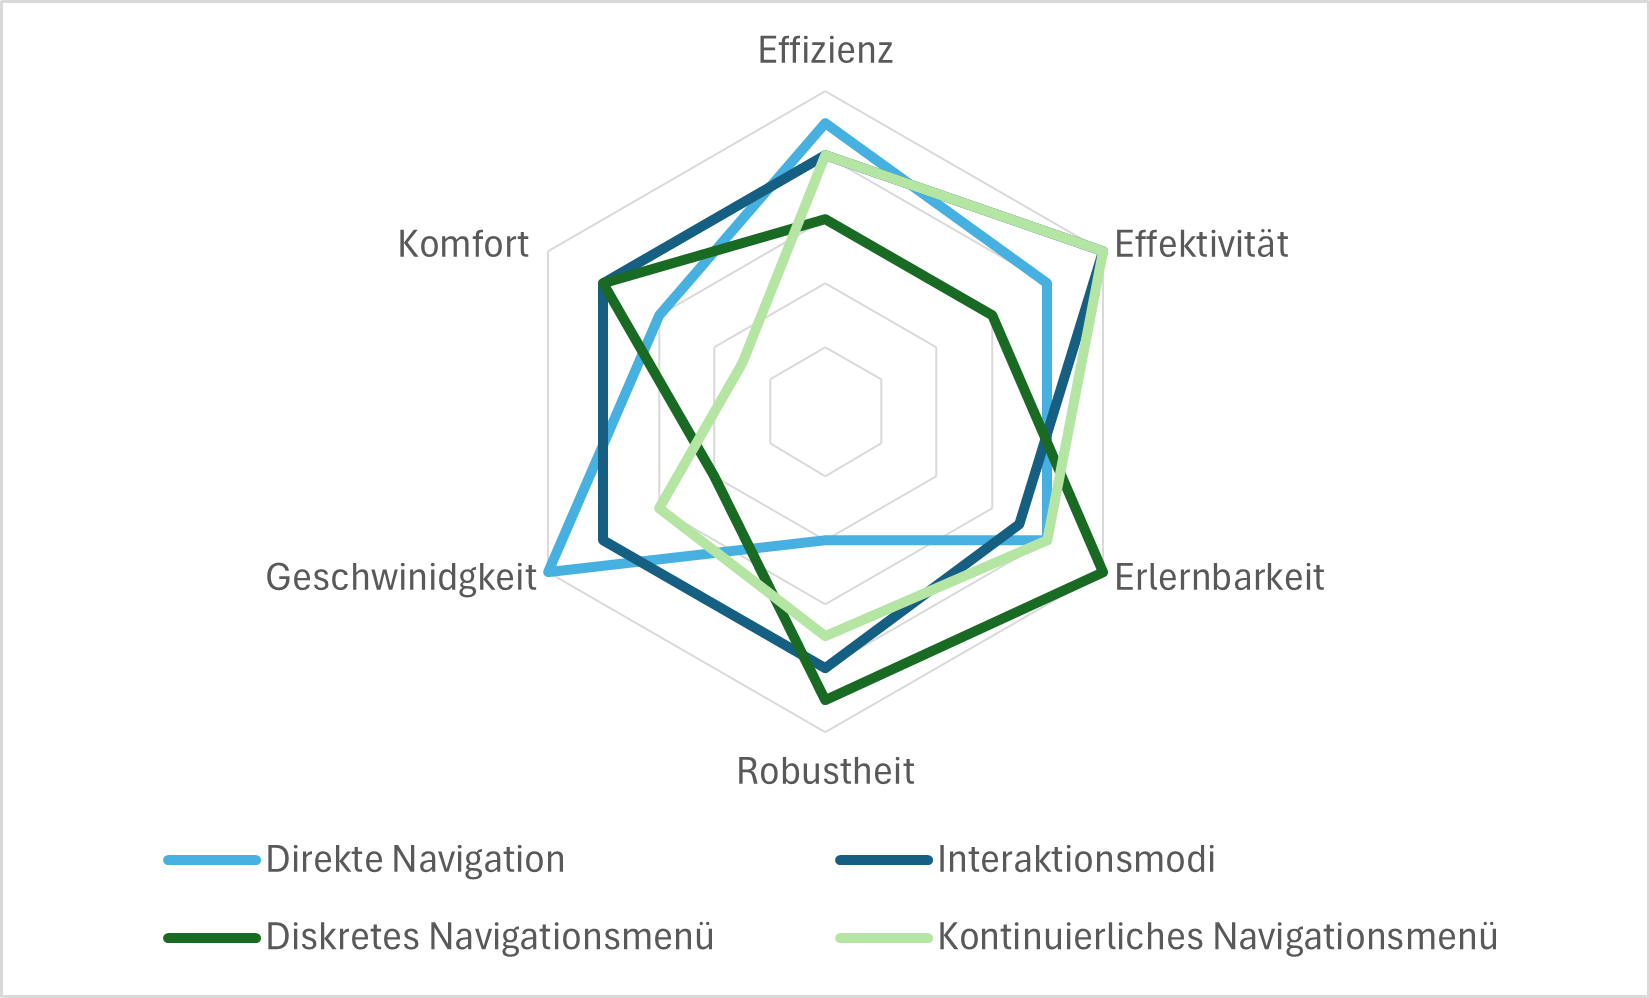
\includegraphics[width=0.75\textwidth]{images/Netzdiagramm-Navigation.png}
    \caption{Visualisierung der Einordnung der Gestaltungsoptionen der Interaktionsaufgabe Navigation}
    \label{fig:Netz-Navigation}
\end{figure}

\textit{Effizienz:}
Die Effizienz der Gestaltungsoptionen der Navigation wird durch den erforderlichen Interaktionsaufwand bestimmt. Der Schwerpunkt liegt hier auf der Anzahl der Eingaben, die zur Durchführung der Navigation erforderlich sind. Die beiden auf dem Cartesian Scanning basierenden Optionen weisen unterschiedliche Effizienzniveaus auf. Die direkte Navigation erfordert lediglich die Festlegung des Schnittpunktes, was eine relativ hohe Effizienz gewährleistet. Allerdings steigt der Interaktionsaufwand bei größeren Rotationswinkeln, da in diesen Fällen mehrere Navigationsschritte erforderlich sein können, um den gewünschten Endpunkt zu erreichen. Die Navigation mit separaten Interaktionsmodi erfordert zusätzlich eine Interaktion, um den Moduswechsel zwischen Navigation und Selektion durchzuführen, was den Aufwand geringfügig erhöht. Daher wird die Effizienz der direkten Navigation etwas höher eingeordnet. 
Bei den Optionen des Item-Scannings hat der gewünschte Rotationswinkel einen erheblichen Einfluss auf die Effizienz. Bei der diskreten Navigation führt ein größerer Winkel zu einer höheren Anzahl von Eingaben, da die Rotation in festen Schritten erfolgt. Dies macht die Methode bei großen Rotationswinkeln weniger effizient. Dagegen erfordert die kontinuierliche Navigation bei kleinen Rotationen einen geringfügig höheren Aufwand, da zwei Eingaben erforderlich sind (eine zum Aktivieren und eine zum Beenden der Navigation). Dieser Mehraufwand wird jedoch bei großen Rotationswinkeln durch die Möglichkeit der kontinuierlichen Navigation kompensiert. Die Effizienz der diskreten Navigation als etwas geringer eingestuft.

\textit{Effektivität:}
Die Effektivität der Gestaltungsoptionen der Navigation wird durch die Genauigkeit bestimmt, mit der ein gewünschter Rotationswinkel erreicht werden kann. Dabei wird insbesondere berücksichtigt, inwieweit die Nutzenden die Navigation kontrollieren und den Rotationswinkel exakt bestimmen können. 
Ein deutlicher Unterschied in der Effektivität zeigt sich bei den Optionen, die auf dem Cartesian Scanning basieren. Die direkte Navigation wird durch die Position und Anzahl der Interaktionselemente in der Szene eingeschränkt. Je mehr Elemente vorhanden sind, desto mehr leidet die Effektivität, da nur Punkte im Raum ausgewählt werden können, an denen sich kein Interaktionselement befindet. Dies schränkt die Kontrolle über den Rotationswinkel erheblich ein. Bei Szenen mit wenigen Interaktionselementen ist dieser Effekt jedoch praktisch vernachlässigbar. Die Navigation mit Interaktionsmodi bietet hingegen eine deutlich höhere Flexibilität, da beliebige Rotationswinkel erreicht werden können.
Auch die Optionen des Item-Scannings unterscheiden sich in ihrer Effektivität. Das Navigationsmenü mit diskreter Rotation erlaubt nur eine begrenzte Anzahl von vorgegebenen Rotationswinkeln. Dies führt dazu, dass die Zielposition nicht immer exakt erreicht werden kann, was wiederum die Effektivität einschränkt. Im Gegensatz dazu bietet die kontinuierliche Rotation durch ihre Flexibilität die Möglichkeit, jeden beliebigen Winkel zu erreichen. Diese Methode gewährleistet somit eine hohe Präzision \citep{10.1145/2159365.2159386}. 

\textit{Erlernbarkeit:} 
Bei der direkten Navigation beim Cartesian Scanning profitieren die Nutzenden von der Vertrautheit mit dem Prinzip aus der Selektion, sodass keine neuen Mechanismen erlernt werden müssen. Allerdings kann die Durchführung der Navigation aufgrund der notwendigen Koordination zwischen Selektion und Navigation anfangs eine gewisse Herausforderung darstellen. Insgesamt wird die Erlernbarkeit daher als hoch eingeschätzt. Die Interaktionsmodi erfordern zusätzlich das Verständnis, wann welcher Modus aktiv ist und wie zwischen den Modi gewechselt wird. Dies könnte eine leichte kognitive Hürde darstellen, insbesondere wenn der Moduswechsel eine andere Art der Eingabe als die Selektion erfordert (z. B. Halten des Schalters oder zwei schnelle Aktivierungen hintereinander). Während das zugrundeliegende Konzept einfach ist, kann die anfängliche Anwendung für neue Benutzer anspruchsvoller sein. Die Erlernbarkeit wird daher als moderat bewertet.
Die diskrete Navigation im Navigationsmenü basiert auf klaren und konsistenten Schritten. Die Nutzenden wählen Buttons aus, die festgelegte Rotationswinkel repräsentieren. Dies macht die Bedienung besonders einfach und einsteigerfreundlich, da keine zusätzlichen Mechanismen erlernt werden müssen. Durch die intuitive Interaktionslogik wird die Erlernbarkeit als sehr hoch bewertet.
Die kontinuierliche Navigation ermöglicht es, die Rotation durch einmalige Selektion eines Buttons zu starten und durch erneute Selektion desselben Buttons zu stoppen. Dieser Mechanismus ist prinzipiell leicht verständlich, kann aber anfangs nicht ganz intuitiv sein, da den Nutzenden möglicherweise nicht klar ist, wie die Rotation wieder gestoppt werden kann. Aufgrund dieser geringen Einstiegshürde wird die Erlernbarkeit als hoch eingeschätzt.

\textit{Robustheit:}
Bei der direkten Navigation (basierend auf dem Cartesain Scanning) können Fehler durch fehlende Abgrenzung zwischen Selektion und Navigation entstehen. Insbesondere in Szenen mit vielen Interaktionselementen oder bei ungenauem Timing kann es zu Verwechslungen kommen, etwa wenn Nutzende ein Element selektieren möchten, die Eingabe jedoch knapp verfehlen. Dies kann dazu führen, dass stattdessen eine Navigation ausgelöst wird, was die Robustheit maßgeblich beeinträchtigt. Die Einführung eines separaten Modus für Navigation und Selektion hingegen minimiert die Wahrscheinlichkeit solcher Fehler und erhöht die Robustheit deutlich. Dennoch können Fehler auftreten, wenn versehentlich der falsche Modus aktiv ist. Bspw. könnte eine Selektion gewünscht sein, während der Navigationsmodus noch aktiv ist. Solche Situationen erfordern eine bewusste Kontrolle durch die Nutzenden, um zwischen den Modi zu wechseln. Insgesamt wird die Robustheit der Interaktionsmodi jedoch als deutlich höher eingeschätzt als die der direkten Navigation.
Ein Navigationsmenü bietet in beiden Varianten eine robuste Kontrolle über die Navigation. Jedoch können Timing-Probleme dazu führen, dass versehentlich in die falsche Richtung navigiert wird. Solche Fehler lassen sich in beiden Varianten korrigieren, jedoch unterscheidet sich der Aufwand je nach Mechanismus. Bei der diskreten Navigation führt eine Fehleingabe lediglich zu einem einzelnen Schritt in die falsche Richtung. Der Fehler kann leicht korrigiert werden, indem im Anschluss die entgegengesetzte Richtung gewählt wird. Die kontinuierliche Navigation erfordert hingegen mehr Aufwand für die Fehlerkorrektur. Nutzende müssen zunächst die aktive Eingabe abbrechen, anschließend die Eingabe für die eigentlich gewünschte Richtung aktivieren und diese wiederum abbrechen, sobald die Korrektur abgeschlossen ist. Dies führt zu einem erhöhten Zeit- und Arbeitsaufwand, was die Robustheit des Verfahrens im Vergleich zur diskreten Navigation verringert \citep{10.1145/2159365.2159386}. 

\textit{Interaktionsgeschwindigkeit:}
Die direkte Navigation wird als die schnellste Option angesehen. Da keine zusätzlichen Schritte für den Wechsel zwischen Selektion und Navigation notwendig sind, kann die Navigation unmittelbar durchgeführt werden. Darüber hinaus ermöglicht die direkte Navigation, einen großen Rotationswinkel mit nur einer Navigation zu erreichen, indem der Schnittpunkt bswp. weit an den Rand des aktuellen Sichtfeldes gesetzt wird. Dies reduziert die Anzahl der notwendigen Navigationen und erhöht damit die Interaktionsgeschwindigkeit. Einschränkungen können jedoch auftreten, wenn die Anzahl oder Position der Interaktionselemente in der Szene die Wahl eines großen Winkels verhindert. Die Option mit getrennten Interaktionsmodi erfordert einen Zwischenschritt, da zwischen Selektion und Navigation gewechselt werden muss, was zusätzliche Zeit in Anspruch nimmt. Nach dem Moduswechsel bietet die Navigation jedoch die gleichen Vorteile wie die direkte Navigation. Darüber hinaus bestehen hier keine Einschränkungen hinsichtlich der Anzahl oder Position der Elemente. 
Die Navigation über ein Navigationsmenü erfordert zunächst das Öffnen des Menüs, was einen Zwischenschritt darstellt, der sich negativ auf die Geschwindigkeit auswirkt. Bei der diskreten Navigation wird die Geschwindigkeit zusätzlich durch die Anzahl der erforderlichen Schritte beeinflusst. Um eine größere Rotation zu erreichen, müssen mehrere Interaktionen nacheinander ausgeführt werden. Dies führt zu einer insgesamt geringeren Geschwindigkeit, insbesondere bei größeren Rotationswinkeln. Im Vergleich zur diskreten Variante ist die kontinuierliche Navigation schneller \citep{10.1145/2159365.2159386}, da eine kontinuierliche Rotation gestartet werden kann, die nur durch eine weitere Interaktion gestoppt werden muss. Dies reduziert die Anzahl der notwendigen Interaktionen und beschleunigt die Navigation insbesondere bei größeren Rotationswinkeln. Jedoch wirkt sich auch hier der Zwischenschritt des Öffnens des Menüs negativ auf die Geschwindigkeit aus. 

\textit{Komfort:}
Der Komfort der Navigation wird maßgeblich durch die erforderliche Konzentration, den allgemeinen kognitiven Aufwand sowie den visuellen Anspruch beeinflusst. Die Optionen, die auf dem Cartesian Scanning basieren, erfordern insgesamt eine präzise Auswahl, um den gewünschten Rotationspunkt zu erreichen. Diese Präzision geht mit einer leicht erhöhten Konzentration einher. Bei der direkten Navigation ist zusätzlich zu berücksichtigen, dass eine unbeabsichtigte Auswahl eines Interaktionselements möglich ist, was den kognitiven Aufwand weiter erhöht. Die Interaktionsmodi-Option reduziert das Risiko von Fehleingaben durch die Trennung von Selektion und Navigation. Dies führt zu einer leicht reduzierten kognitiven Belastung im Vergleich zur direkten Navigation. Die visuelle Komplexität der Szene wird durch das Hinzufügen zusätzlichenr Interaktionselemente für das Navigationsmenü leicht erhöht. Die diskrete Navigation mit vorgegebenen Rotationswinkeln erfordert insgesamt die geringste Konzentration, da die Interaktion sehr konsistent ist. Dadurch wird die kognitive Belastung minimiert.
Die kontinuierliche Navigation benötigt ein gewisses Timing, um die Rotation im gewünschten Moment zu stoppen. Dies erfordert eine erhöhte Konzentration im Vergleich zur diskreten Option. Darüber hinaus besteht bei einer durchgängigen Rotation der First-Person-Kamera ein erhöhtes Risiko für Motion Sickness, was den Komfort weiter beeinträchtigen kann \citep{10.1007/s10055-020-00425-x, 8797722}.


{\normalfont \bfseries Interaktionskomponenten:} 

\textbf{1. Display}

Folgend werden die erarbeiteten Gestaltungsoptionen für die Komponente Display anhand der definierten Parameter eingeordnet. Die Ergebnisse dieser Einordnung sind in \autoref{fig:Netz-Display} zusammenfassend visualisiert.

\begin{figure}[tbh]
    \centering
    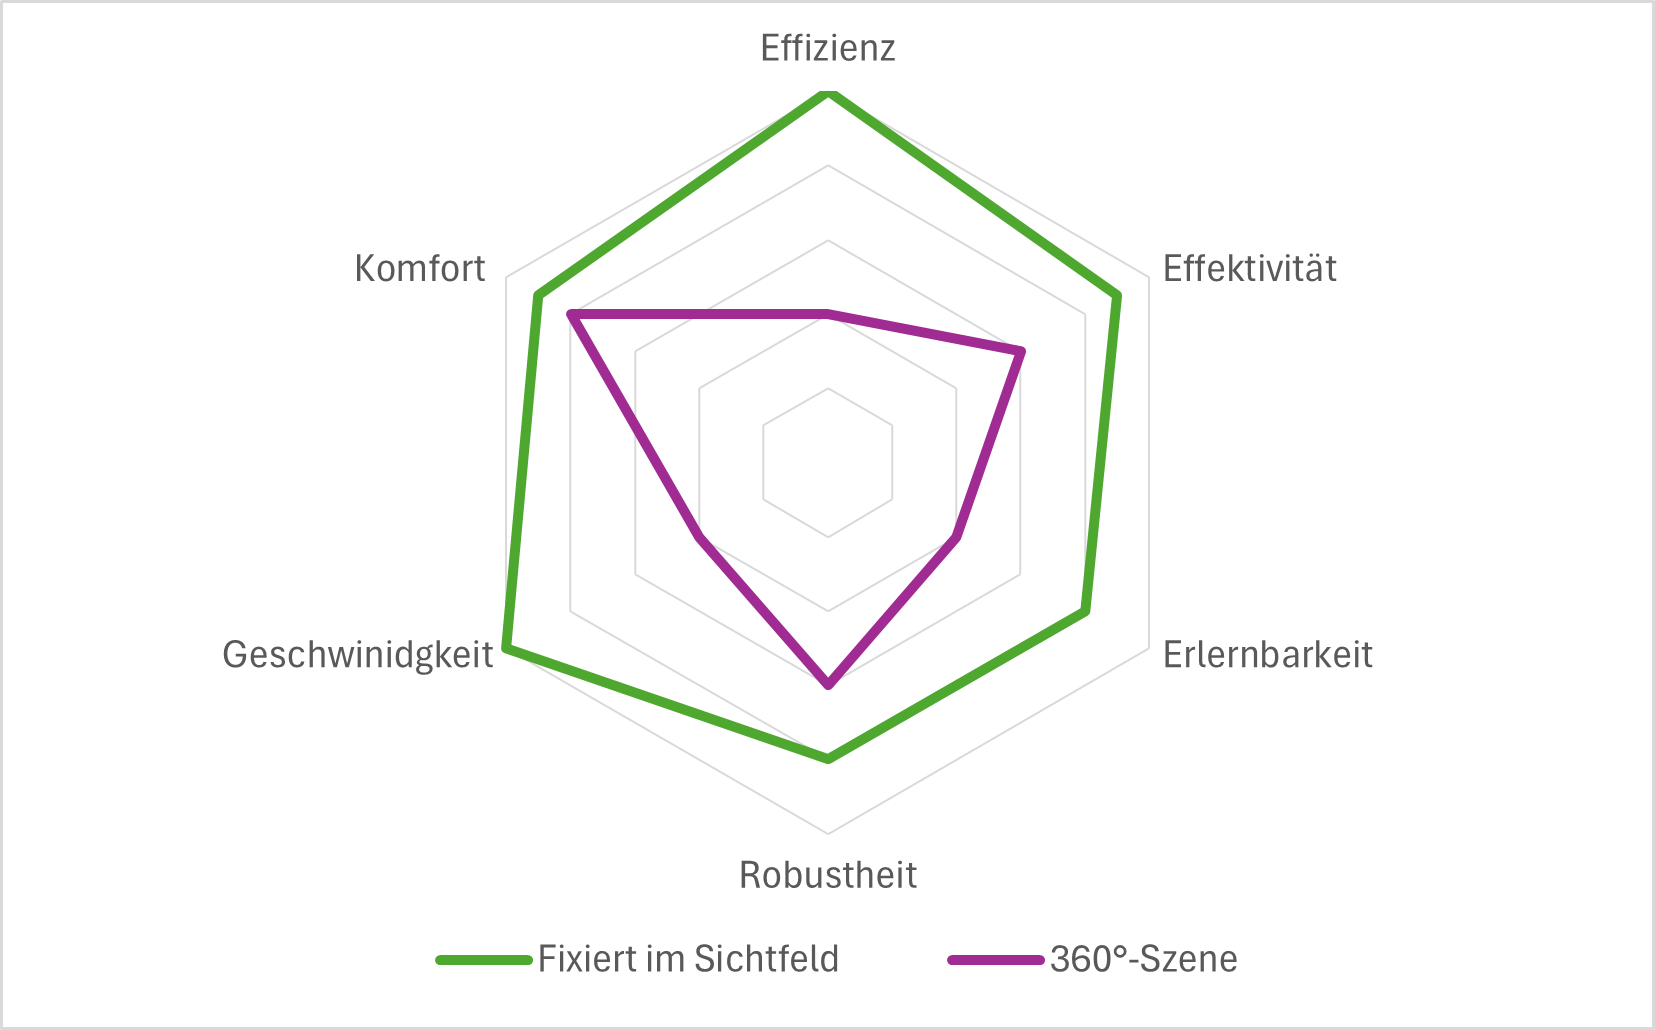
\includegraphics[width=0.75\textwidth]{images/Netzdiagramm-Display.png}
    \caption{Visualisierung der Einordnung der Gestaltungsoptionen der Interaktionskomponente Display}
    \label{fig:Netz-Display}
\end{figure}

\textit{Effizienz:}
Die Effizienz der verschiedenen Optionen zur Darstellung des Scanning-Verfahrens in der virtuellen Umgebung wird hinsichtlich des erforderlichen Aufwands analysiert. Es zeigt sich, dass der Einfluss der Display-Optionen von der Art des Scanning-Verfahrens abhängt.
Sowohl beim Automatic Item Scanning als auch beim Cartesain Scanning ist der Aufwand unabhängig davon, ob das Scanning-Verfahren auf das Sichtfeld beschränkt oder auf die gesamte Szene ausgeweitet wird. Bei beiden Verfahren erfolgt das Scanning automatisiert und die präsentierte Auswahl (Item: hervorgehobenes Element, Cartesain: Position der Linien) wird durch Aktivierung des Schalters ausgewählt. Im Gegensatz dazu zeigt sich bei Step und Inverse Item Scanning ein deutlicher Einfluss der Display-Optionen. Wird das Scanning auf die gesamte Szene ausgeweitet, werden alle Interaktionselemente unabhängig von ihrer Position in das Scan-Set einbezogen. Dadurch erhöht sich die Anzahl der zu durchlaufenden Elemente. Beim Step Item Scanning erhöht sich dadurch die Anzahl der erforderlichen Schalterbetätigungen und beim Inverse Item Scanning wird ein längeres Halten des Schalters erforderlich. Dies führt zu einem deutlich erhöhten Aufwand und damit zu einer geringen Effizienz. Eine Beschränkung des Scan-Sets auf Elemente im Sichtfeld hingegen reduziert die Anzahl der zu durchlaufenden Interaktionselemente und damit den erforderlichen Aufwand bei beiden Verfahren deutlich. Dies ist insbesondere bei Szenen mit vielen Interaktionselementen entscheidend. 

\textit{Effektivität:}
Die Fixierung des Scanning-Verfahren an das Sichtfeld des Nutzenden ermöglicht eine feinere Kontrolle des Scanning, da der Scan-Bereich immer visuell verfolgt werden kann, was sich wiederum positiv auf die Effektivität auswirkt. Ist das Scanning-Verfahren auf die gesamte Szene ausgeweitet, tritt der gegenteilige Effekt ein. In diesem Fall wird eine präzise Steuerung erschwert, da der Scan-Bereich nicht vollständig visuell erfasst werden kann, was insbesondere bei komplexen Szenen zu Verwirrung und damit zu unpräziseren Interaktionen führen kann. Die Effektivität wird daher für die Fixierung als hoch bewertet und für die Ausweitung auf den gesamten 360°-Bereich der Szene als moderat. 

\textit{Erlernbarkeit:} 
Bei der Fixierung im Sichtfeld bleibt der gesamte Scan-Vorgang im sichtbaren Bereich, was das visuelle Feedback erleichtert. Die Nutzenden können jederzeit erkennen, ob der Scan-Vorgang aktiv ist und diesen verfolgen. Dies erleichtert nicht nur den Einstieg in die Nutzung, sondern reduziert auch das Risiko von Missverständnissen oder Fehleingaben. Im Falle einer Fehleingabe kann diese direkt visuell nachvollzogen und ggf. korrigiert werden. Aufgrund dieser Transparenz wird die Erlernbarkeit dieser Option als hoch bewertet.
Wird das Scanning-Verfahren auf die gesamte Szene ausgeweitet, erfordert dies ein höheres Maß an Verständnis für den Systemzustand, da der Scan-Vorgang auch außerhalb des Sichtfeldes stattfinden kann. Fehlerhafte Schalterbetätigungen können in diesem Fall Systemreaktionen auslösen, die für die Nutzenden nicht unmittelbar nachvollziehbar sind. Dies erschwert das Erlernen und erfordert zusätzliche Rückmeldesysteme, um den Status des Scans verständlich zu machen. Die Erlernbarkeit wird daher als geringer eingestuft. 

\textit{Robustheit:}
Die Fixierung des Scanning-Verfahren auf das Sichtfeld ermöglicht es den Nutzenden, den Scan-Vorgang durch gezielte Kopfbewegungen zu beeinflussen. Diese Möglichkeit kann insbesondere beim Cartesian Scanning die Robustheit erhöhen, da kleinere Ungenauigkeiten durch bewusste Kopfbewegungen korrigiert werden können. Dies setzt allerdings voraus, dass die Nutzenden dazu in der Lage sind, Kopfbewegungen präzise und kontrolliert vorzunehmen. Für Personen mit eingeschränkter motorischer Kontrolle könnte diese Abhängigkeit von der Kopfbewegung unter Umständen problematisch sein und die Robustheit der Interaktion verringern. Unbeabsichtigte Verschiebungen des Scan-Vorgangs durch unkontrollierte Kopfbewegungen oder ungenaue Steuerung können dazu führen, dass Interaktionselemente verfehlt werden. Dies erhöht das Risiko von Navigations- oder Selektionsfehlern. Trotz dieser möglichen Nachteile bleibt die visuelle Rückmeldung innerhalb des Sichtfeldes ein stabilisierender Faktor, der die Nachvollziehbarkeit von Fehlern und deren Korrektur erleichtert. 
Die Integration des Scanning-Verfahren in die gesamte Szene eliminiert die Abhängigkeit von Kopfbewegungen und verhindert somit unbeabsichtigte Verschiebungen des Scannings durch unkontrollierte Bewegungen und erhöht damit die Robustheit des Systems. Diese Option birgt jedoch ein erhöhtes Risiko unbeabsichtigter Selektionen, da der Scan außerhalb des Sichtfeldes stattfinden kann und für die Nutzenden visuell nicht jederzeit nachvollziehbar ist. Bei den Scanning-Verfahren Automatic und Inverse Item Scanning sowie beim Cartesian Scanning können außerdem schneller Timing-Fehler entstehen, wenn der Scan-Vorgang von außerhalb des Sichtfeldes in den Sichtbereich übergeht. In diesem Fall könnte die Reaktionszeit des Nutzenden nicht ausreichen, um das Zielelement rechtzeitig zu selektieren. 

\textit{Interaktionsgeschwindigkeit:}
Die Interaktionsgeschwindigkeit der beiden Display-Optionen unterscheidet sich deutlich. Die Option mit fixiertem Scanning im Sichtfeld bietet deutliche Vorteile in der Interaktionsgeschwindigkeit. Da hier beim Item Scanning nur die Elemente im Sichtfeld gescannt werden, ist die Größe des Scan-Sets begrenzt, was zu einem schnelleren Durchlauf der Sequenz und damit zu einer schnelleren Interaktionsgeschwindigkeit führt. Beim Cartesian Scanning ist die Bewegung der Linien auf einen kleinen Bereich beschränkt, sodass Wartezeiten reduziert werden können. Darüber hinaus können beim Cartesian Scanning Kopfbewegungen (sofern möglich) dazu genutzt werden, die Scan-Linien näher an das gewünschte Zielelement zu bringen, was die Interaktionsgeschwindigkeit beschleunigt. Insgesamt führt die Kombination aus kleiner Größe des Scan-Sets und aktiver Beeinflussbarkeit durch Kopfbewegungen zu einer hohen Interaktionsgeschwindigkeit.
Die auf die gesamte Szene erweiterte Option zeigt eine geringere Interaktionsgeschwindigkeit, insbesondere beim Item Scanning. Da hier alle Elemente der Szene unabhängig von ihrer Position im Sichtfeld berücksichtigt werden, nimmt die Größe des Scan-Sets deutlich zu. Dies führt zu einer Verzögerung, da der Scan-Vorgang mehr Zeit benötigt, um alle Elemente sequentiell zu durchlaufen. Beim Cartesian Scanning ist die Interaktionsgeschwindigkeit ebenfalls niedriger, da die Bewegung der Scan-Linien unabhängig von der Blickrichtung stattfindet und somit mehr Zeit in Anspruch nimmt. Außerdem ist es nicht möglich, den Scan-Vorgang durch Kopfbewegungen gezielt zu beschleunigen. 

\textit{Komfort:}
Der Komfort der beiden Display-Optionen unterscheidet sich deutlich hinsichtlich der erforderlichen Konzentration, der visuellen Komplexität und der motorischen Ermüdung.
Die Fixierung des Scan-Vorgangs im Sichtfeld erfordert ein höheres Maß an Konzentration, da selbst minimale Kopfbewegungen einen direkten Einfluss auf den Scan-Vorgang haben. Dies kann zu ungewollten Verschiebungen führen. Darüber hinaus kann die Kombination von Kopfbewegung und Scanning zu visuellen Irritationen führen, insbesondere wenn die Bewegung der Scan-Linien aufgrund der Kopfbewegung schneller oder unregelmäßiger erscheint. Ein Vorteil dieser Option liegt jedoch in der potenziell geringeren motorischen Ermüdung, da durch die Beschränkung auf das Sichtfeld das Scan-Set verkleinert werden kann, wodurch die Anzahl der erforderlichen Interaktionen reduziert wird, insbesondere bei Verfahren wie Step und Inverse Item Scanning. 
Die Option, das Scanning auf die gesamte 360°-Szene zu erstrecken, bietet hinsichtlich der Konzentration einen deutlichen Vorteil, da Kopfbewegungen keinen Einfluss auf den Scan-Vorgang haben. Dies minimiert die Anforderungen an die Aufmerksamkeit und sorgt für einen gleichmäßigen Ablauf des Scannings, was den Komfort erhöht. Auch die visuelle Komplexität ist vergleichsweise gering, da die Bewegung des Scannings unabhängig von äußeren Einflüssen erfolgt und somit vorhersehbar bleibt. Allerdings zeigt diese Option Schwächen bei der motorischen Ermüdung, insbesondere im Zusammenhang mit Step und Inverse Item Scanning. Die größere Größe des Scan-Sets erfordert eine höhere Anzahl von Interaktionen oder ein längeres Halten des Schalters, was schnell zu Ermüdung führen kann. 

\textbf{2. Transition} 

Im Folgenden erfolgt die Einordnung der erarbeiteten Gestaltungsoptionen für die Komponente Transition anhand der definierten Parameter. Die Ergebnisse dieser Einordnung sind in \autoref{fig:Netz-Transition} zusammenfassend dargestellt. 

\begin{figure}[tbh]
    \centering
    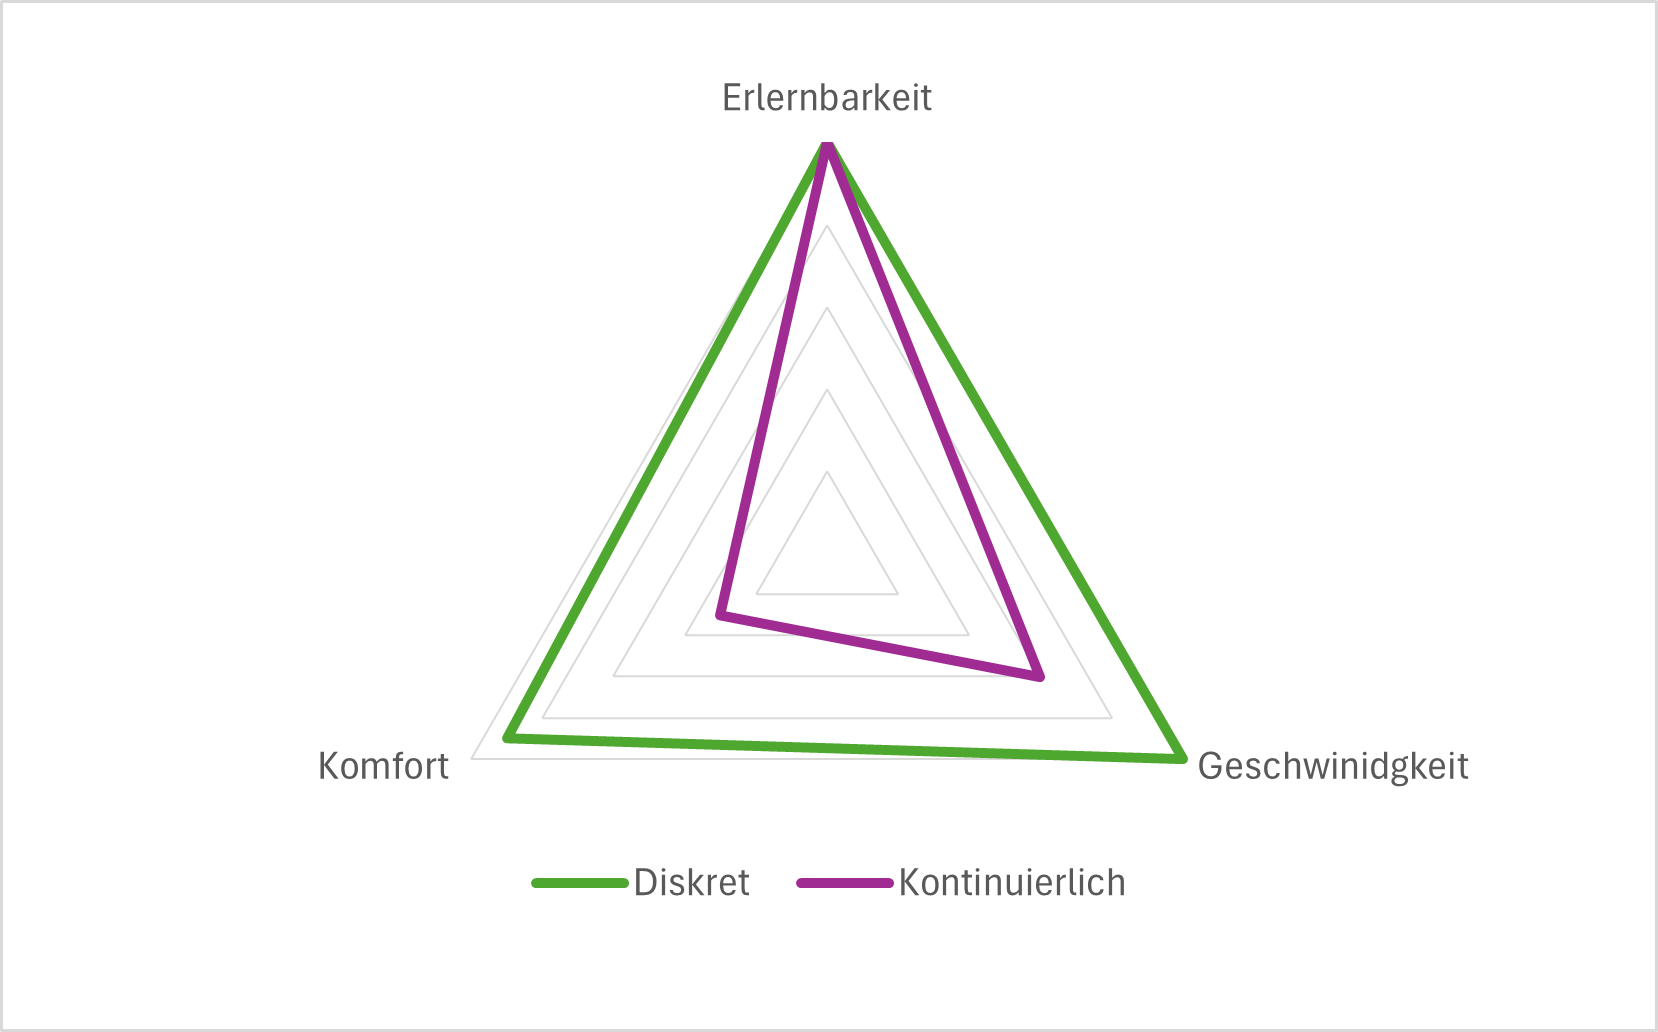
\includegraphics[width=0.75\textwidth]{images/Netzdiagramm-Transition.png}
    \caption{Visualisierung der Einordnung der Gestaltungsoptionen der Interaktionskomponente Transition}
    \label{fig:Netz-Transition}
\end{figure}

\textit{Effizienz:}
Die Effizienz der Interaktion, gemessen am notwendigen Aufwand, wird durch die Gestaltung der Transition kaum beeinflusst. Beide Optionen führen die Rotation mit einem vergleichbaren Aufwand durch, da die grundlegende Interaktion zur Auslösung der Rotation identisch bleibt.

\textit{Effektivität:} 
Die Effektivität der Interaktion, gemessen an der Präzision des Rotationswinkel, wird durch die Gestaltung der Transition nicht beeinflusst. Der exakte Rotationswinkel wird durch die Navigation bestimmt, während die Transition lediglich den visuellen Übergang zwischen Ausgangs- und Zielposition gestaltet.

\textit{Erlernbarkeit:}
Die Erlernbarkeit der Optionen ist als hoch einzuschätzen, da beide Ansätze bereits in etablierten VR-Anwendungen implementiert werden und somit den Nutzenden einen Wiedererkennungswert bieten.
%BEISPIELE EINBINDEN! 

\textit{Robustheit:}
Die Optionen zur Gestaltung der Transition haben keinen bedeutenden Einfluss auf das Auftreten oder die Vermeidung von Fehlern und somit keinen direkten Einfluss auf die Robustheit. Es kann davon ausgegangen werden, dass beide Optionen stabile und zuverlässige Transitionen darstellen, da sie bereits häufig in VR-Anwendungen implementiert sind. Einflüsse auf die Robustheit können sich ggf. ergeben, wenn durch die Art der Transition Motion Sickness auftritt und die Nutzenden in Folge dessen dazu neigen, eher Fehler zu machen. 

\textit{Interaktionsgeschwindigkeit:}
Die Optionen für die Transition unterscheiden sich in der Interaktionsgeschwindigkeit. Direkte Rotation bietet eine schnellere Interaktionsgeschwindigkeit, da die Kamera ohne Übergangszeit unmittelbar in die gewünschte Position gebracht wird. Die kontinuierliche Rotation hingegen ist aufgrund der Übergangszeit langsamer. Hier findet eine Bewegung der Kamera über die Zeit statt. Daher benötigt diese Transition länger, um die Zielposition zu erreichen \citep{8797722}. Der Unterschied zwischen den Interaktionszeiten wird durch die Geschwindigkeit der Kamerabewegung und die Größe des gewählten Rotationswinkels beeinflusst. Eine Rotation um einen großen Rotationswinkel erfordert mehr Zeit. Bei einer Direkten Rotation ist die Geschwindigkeit hingegen konstant und nicht von anderen Faktoren abhängig. 

\textit{Komfort:}
Die Optionen für die Transition unterscheiden sich deutlich in Bezug auf den Komfort, insbesondere im Hinblick auf die Auswirkungen auf die Wahrscheinlichkeit für das Auftreten von Motion Sickness und die räumliche Wahrnehmung.
Die kontinuierliche Rotation ahmt die natürliche Bewegung des Kopfes nach und wird daher als realistischer empfunden \citep{8797722}. Dies kann das räumliche Bewusstsein der Nutzenden verbessern \citep{10.1145/3441852.3471230}. Allerdings birgt die Kontinuierliche Transition ein sehr hohes Risiko für das Auftreten von Motion Sickness \citep{10.1007/s10055-020-00425-x, 8797722}, was den Komfort deutlich mindert.
Im Gegensatz dazu ist das Risiko von Motion Sickness bei der direkten Rotation vergleichsweise gering. Allerdings kann die plötzliche Änderung des Sichtfeldes dazu führen, dass die Nutzenden kurzzeitig die räumliche Orientierung verlieren und sich in ihrer Umgebung neu orientieren müssen \citep{10.1145/3441852.3471230}. 

\textbf{3. Initialisierung} 

Im Folgenden werden die erarbeiteten Gestaltungsoptionen für die Komponente Initialisierung anhand der definierten Parameter eingeordnet. Die Ergebnisse dieser Einordnung sind in \autoref{fig:Netz-Initialisierung}zusammenfassend dargestellt. 

\begin{figure}[tbh]
    \centering
    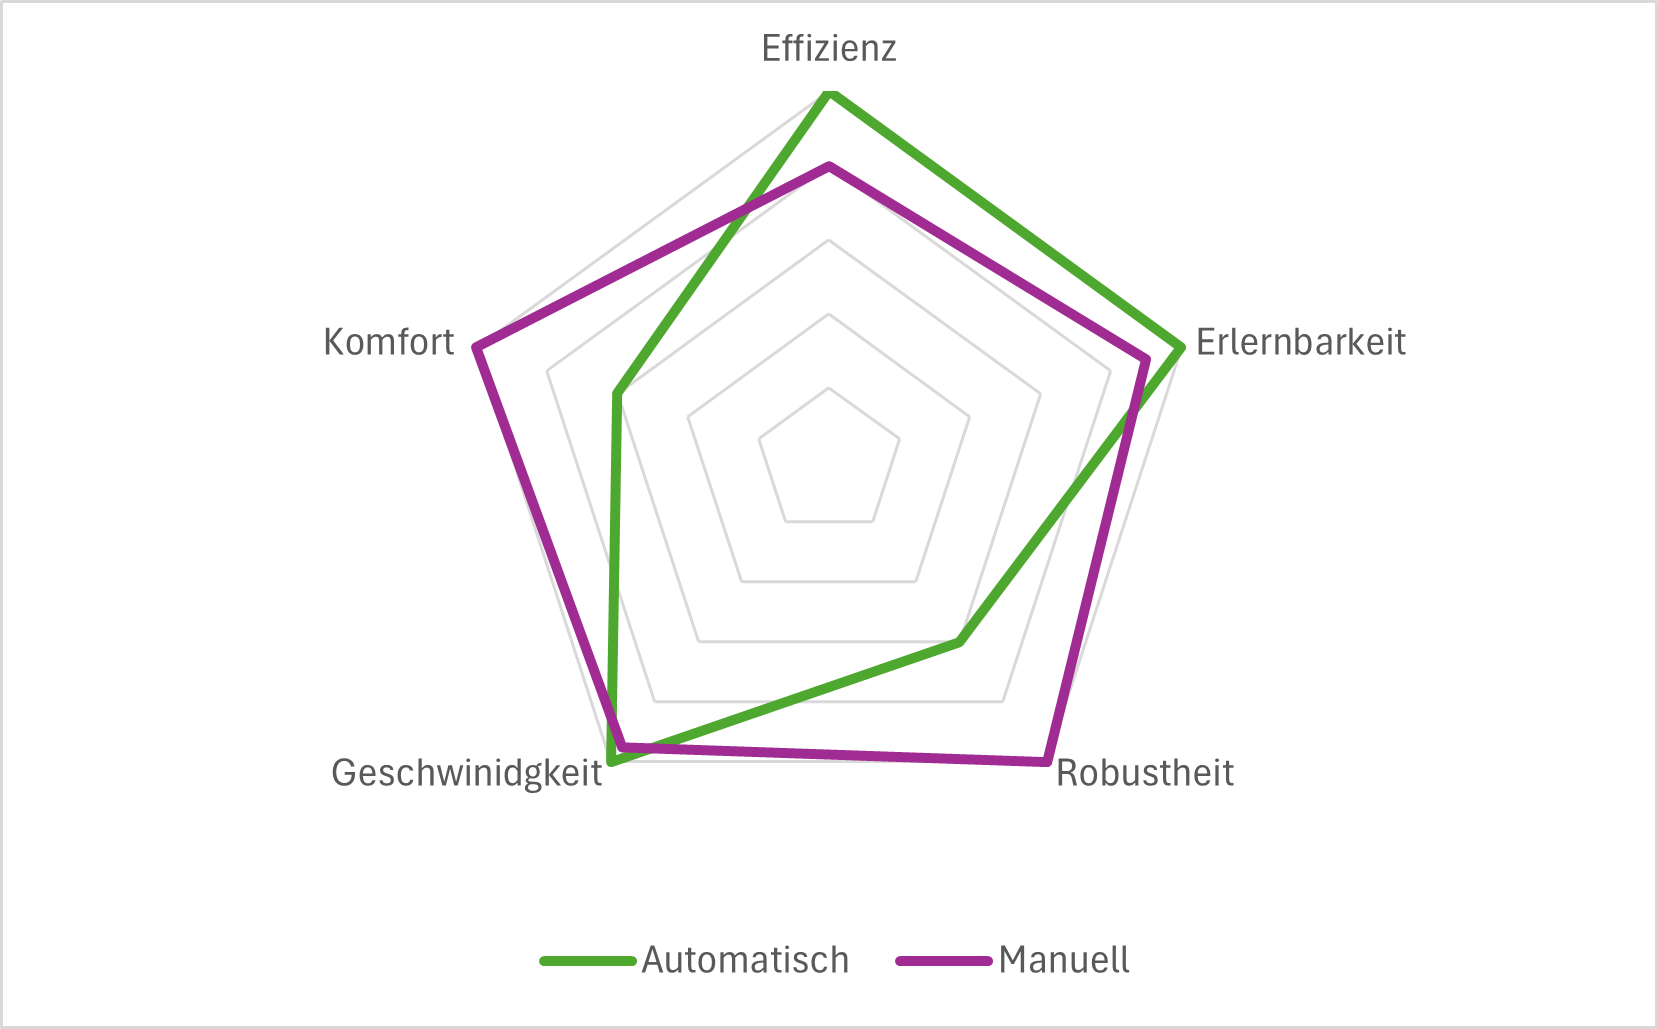
\includegraphics[width=0.75\textwidth]{images/Netzdiagramm-Initialisierung.png}
    \caption{Visualisierung der Einordnung der Gestaltungsoptionen der Interaktionskomponente Initialisierung}
    \label{fig:Netz-Initialisierung}
\end{figure}

\textit{Effizienz:}
Die Effizienz der beiden Initialisierungsoptionen unterscheidet sich nur geringfügig. Die automatische Aktivierung ermöglicht eine kontinuierliche Verfügbarkeit des Scanning-Verfahrens, sodass Interaktionen jederzeit ohne vorherige Aktivierung durchgeführt werden können. Dies reduziert den Aufwand und erhöht die sofortige Bereitschaft für Interaktionen. Die manuelle Initialisierung erfordert hingegen einen zusätzlichen Zwischenschritt, bei dem die Nutzenden das Scanning-Verfahren aktivieren. Obwohl dieser Schritt allein nur minimalen Aufwand erfordert, kann er in Szenarien, in denen häufige Aktivierungen erforderlich sind, den erforderlichen Gesamtaufwand erhöhen. 

\textit{Effektivität:}
Die Effektivität wird durch die Wahl der Initialisierungsoption kaum beeinflusst. Der Initialisierungsschritt bei der manuellen Aktivierung hat keinen Einfluss auf die Genauigkeit oder den Erfolg der Interaktion selbst, sondern nur auf den Beginn des Prozesses.

\textit{Erlernbarkeit:}
Die Erlernbarkeit der automatischen Aktivierung ist besonders hoch, da keine zusätzlichen Schritte oder Erklärungen erforderlich sind. Das Scanning-Verfahren wird automatisch gestartet und läuft kontinuierlich ab, was für die Nutzenden direkt ersichtlich ist. Im Gegensatz dazu erfordert die manuelle Initialisierung eine kurze Einführung, um den Aktivierungsmechanismus zu erklären. Da dies im Allgemeinen durch eine einfache Eingabe erfolgt, bleibt die zusätzliche kognitive Belastung gering und die Erlernbarkeit wird nur minimal beeinflusst.

\textit{Robustheit:}
Die Robustheit der manuellen Initialisierung wird als höher eingestuft, da das Scanning-Verfahren erst nach einer bewussten Aktivierung durch den Nutzenden startet. Dies minimiert das Risiko unbeabsichtigter Eingaben oder Fehlselektionen, die bei einer kontinuierlichen Aktivierung häufiger auftreten könnten. Die automatische Aktivierung hingegen erhöht die Wahrscheinlichkeit von Fehlselektionen, da das Scanning dauerhaft aktiv ist und unbeabsichtigte oder doppelte Eingaben potenziell direkt eine Interaktion auslösen.

\textit{Interaktionsgeschwindigkeit:}
Die Interaktionsgeschwindigkeit wird bei einem durchgehend aktivierten Scanning-Verfahren leicht positiv beeinflusst, da keine zusätzliche Initialisierung erforderlich ist. Die Nutzenden können direkt mit der Interaktion beginnen, was eine schnelle Ausführung ermöglicht. Im Vergleich dazu führt die manuelle Initialisierung zu einem minimalen Zeitverlust durch den zusätzlichen Zwischenschritt, der in der praktischen Anwendung jedoch vermutlich unerheblich ist.

\textit{Komfort:}
Der Komfort ist je nach Initialisierungsoption des Scanning-Verfahrens unterschiedlich. Eine automatische Aktivierung führt zu einer permanenten Überlagerung der Szene mit dem Scanning-Verfahren, was von den Nutzenden als störend empfunden werden könnte. Dies erhöht die visuelle Komplexität und erfordert eine stärkere Konzentration auf den eigentlichen Inhalt der Szene. Darüber hinaus könnte die kontinuierliche Bewegung des Scanning-Verfahrens bei längerer Nutzung ermüdend wirken und die immersive Wahrnehmung der Szene beeinträchtigen.
Im Gegensatz dazu bietet die manuelle Initialisierung den Nutzenden die Möglichkeit, das Scanning-Verfahren nur bei Bedarf zu aktivieren. Dadurch wird die visuelle Komplexität der Szene reduziert, was zu einer entspannteren Nutzung und einer besseren Fokussierung auf wesentliche Inhalte beitragen könnte. Insbesondere bei längerer Nutzung oder bei Szenen mit komplexen visuellen Informationen kann dadurch der Komfort gesteigert werden. Darüber hinaus könnte die zeitweise Deaktivierung des Scanning-Verfahrens ein tieferes Eintauchen in die virtuelle Szene ermöglichen, da weniger Ablenkung durch visuelle Elemente besteht.

\section{Ableitung der finalen Konzepte}
% Wie wurde die Auswahl getroffen (Kriterien), welche Konzepte mit welchen Ausprägungen ergeben sich daraus, welche Strategien werden angewandt, um Problemen entgegenzuwirken (z.b. Item Animation um Scan-Reihenfolge zu visualisieren und damit mehr Orientierung zu liefern, beschränkung Scanning auf Ebenen (Im Menü wird nur Menü durchlaufen, im Dialog nur Antwortmöglichkeiten etc), zurück-option bei Menü; bei Cartesain: wechsel des Modus durch gedrückt halten, verschiedene farben der Scan-Linien um den Modus zu visualiseren, Linien leer durchlaufen lassen bricht den Scan ab, nach einem durchlauf gehts wieder von vorne los)

Die Festlegung der zwei finalen Konzepte für die zwei zu entwickelnden Interaktionsschnittstellen erfolgt auf Basis der detaillierten Bewertung der Gestaltungsoptionen, wie sie im vorangegangenen Abschnitt erarbeitet wurden. Dabei wird diejenige Option bevorzugt, die in der Gesamtbetrachtung die positivsten Bewertungen aufweist und ein ausgewogenes Verhältnis zwischen Effektivität, Effizienz, Robustheit, Interaktionsgeschwindigkeit, Erlernbarkeit und Komfort bietet.
Der Komfort steht dabei besonders im Vordergrund, da das Auftreten von Motion Sickness einen erheblichen Einfluss auf die generelle Nutzbarkeit und Akzeptanz der Interaktionsschnittstellen hat. In den Bereichen, in denen keine der Optionen hinsichtlich der Parameter eindeutig überlegen ist, wird dieser Aspekt entsprechend stärker gewichtet. Damit soll sichergestellt werden, dass die ausgewählten Konzepte nicht nur funktional, sondern auch für die Nutzenden angenehm und zugänglich sind.


{\normalfont \bfseries 1. Konzept: (Automatic) Item Scanning} 

\begin{figure}[tbh]
    \centering
    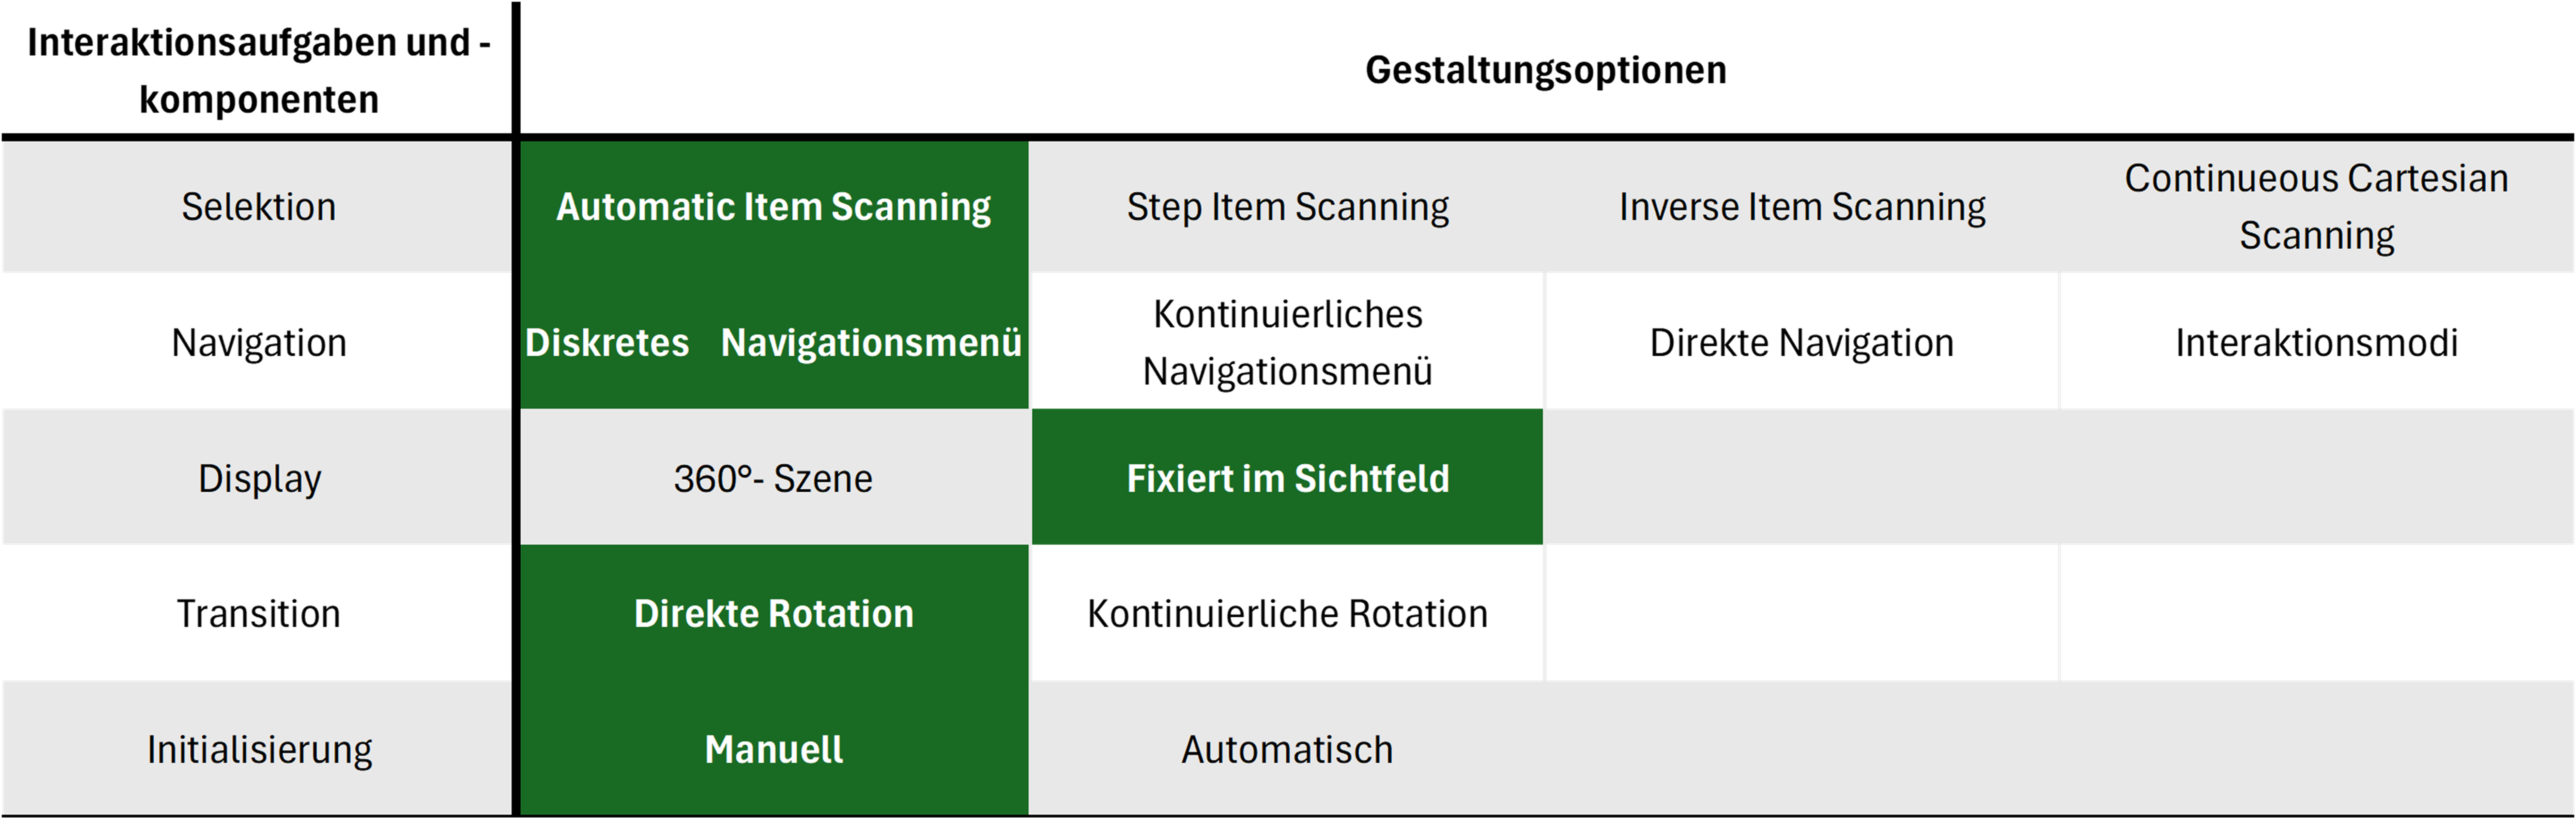
\includegraphics[width=0.95\textwidth]{images/MorphKasten-Item.png}
    \caption{Darstellung des Konzept 1: Item Scanning}
    \label{fig:MorphKasten-Item}
\end{figure}

Das erste Konzept basiert auf dem Automatic Item Scanning , das sich durch eine vergleichsweise ausgewogene Bewertung in allen Parametern auszeichnet. Es erzielt zwar nicht in allen Kriterien die besten Ergebnisse, weist aber insgesamt die geringsten Defizite auf und bietet eine solide Grundlage für eine effektive und effiziente Interaktion. Die Navigation erfolgt über ein diskretes Navigationsmenü. Hier war die Bewertung der Optionen nicht eindeutig, jedoch überzeugt die diskrete Navigation insbesondere durch ihre deutlich geringeren Defizite bezüglich des Komforts. Dies ist insbesondere auf das geringere Risiko von Motion Sickness im Vergleich zur kontinuierlichen Navigation zurückzuführen.

Das Scanning-Verfahren wird im Sichtfeld der Nutzenden fixiert, da diese Gestaltungsoption der Komponente Display hinsichtlich aller Parameter durch klare Vorteile überzeugt. Ebenso wird eine diskrete Rotation als Transitionsmethode verwendet, da diese sowohl hinsichtlich des Komforts als auch der Interaktionsgeschwindigkeit überzeugt. Die Initialisierung des Scanning-Verfahrens erfolgt manuell, da diese Variante im Vergleich zur automatischen Aktivierung zwar eine geringere Effizienz aufweist, aber insbesondere hinsichtlich Komfort und Robustheit Vorteile bietet.
Die für dieses Konzept ausgewählten Gestaltungsoptionen der Interaktionsaufgaben und -komponenten sind in \autoref{fig:MorphKasten-Item} zusammenfassend dargestellt.

Um mögliche Schwächen der gewählten Gestaltungsoptionen zu minimieren, wird das Scanning-Verfahren so gestaltet, dass es nur die Elemente einer aktiven Ebene durchläuft, z. B. nur die Antwortoptionen eines geöffneten Dislog-Elements. Dies reduziert die Größe des Scan-Sets und verkürzt die Interaktionszeit. Zusätzlich wird eine "Zurück"-Option integriert, die es erlaubt, den Dialog durch erneutes Auswählen wieder zu schließen. Um die Orientierung zu verbessern und eine klare Visualisierung der Scan-Reihenfolge zu gewährleisten, wird das Scanning-Verfahren durch eine Animation ergänzt, die die Scan-Reihenfolge verdeutlicht und dadurch die Robustheit erhöht.

{\normalfont \bfseries 2. Konzept: Cartesian Scanning}

\begin{figure}[tbh]
    \centering
    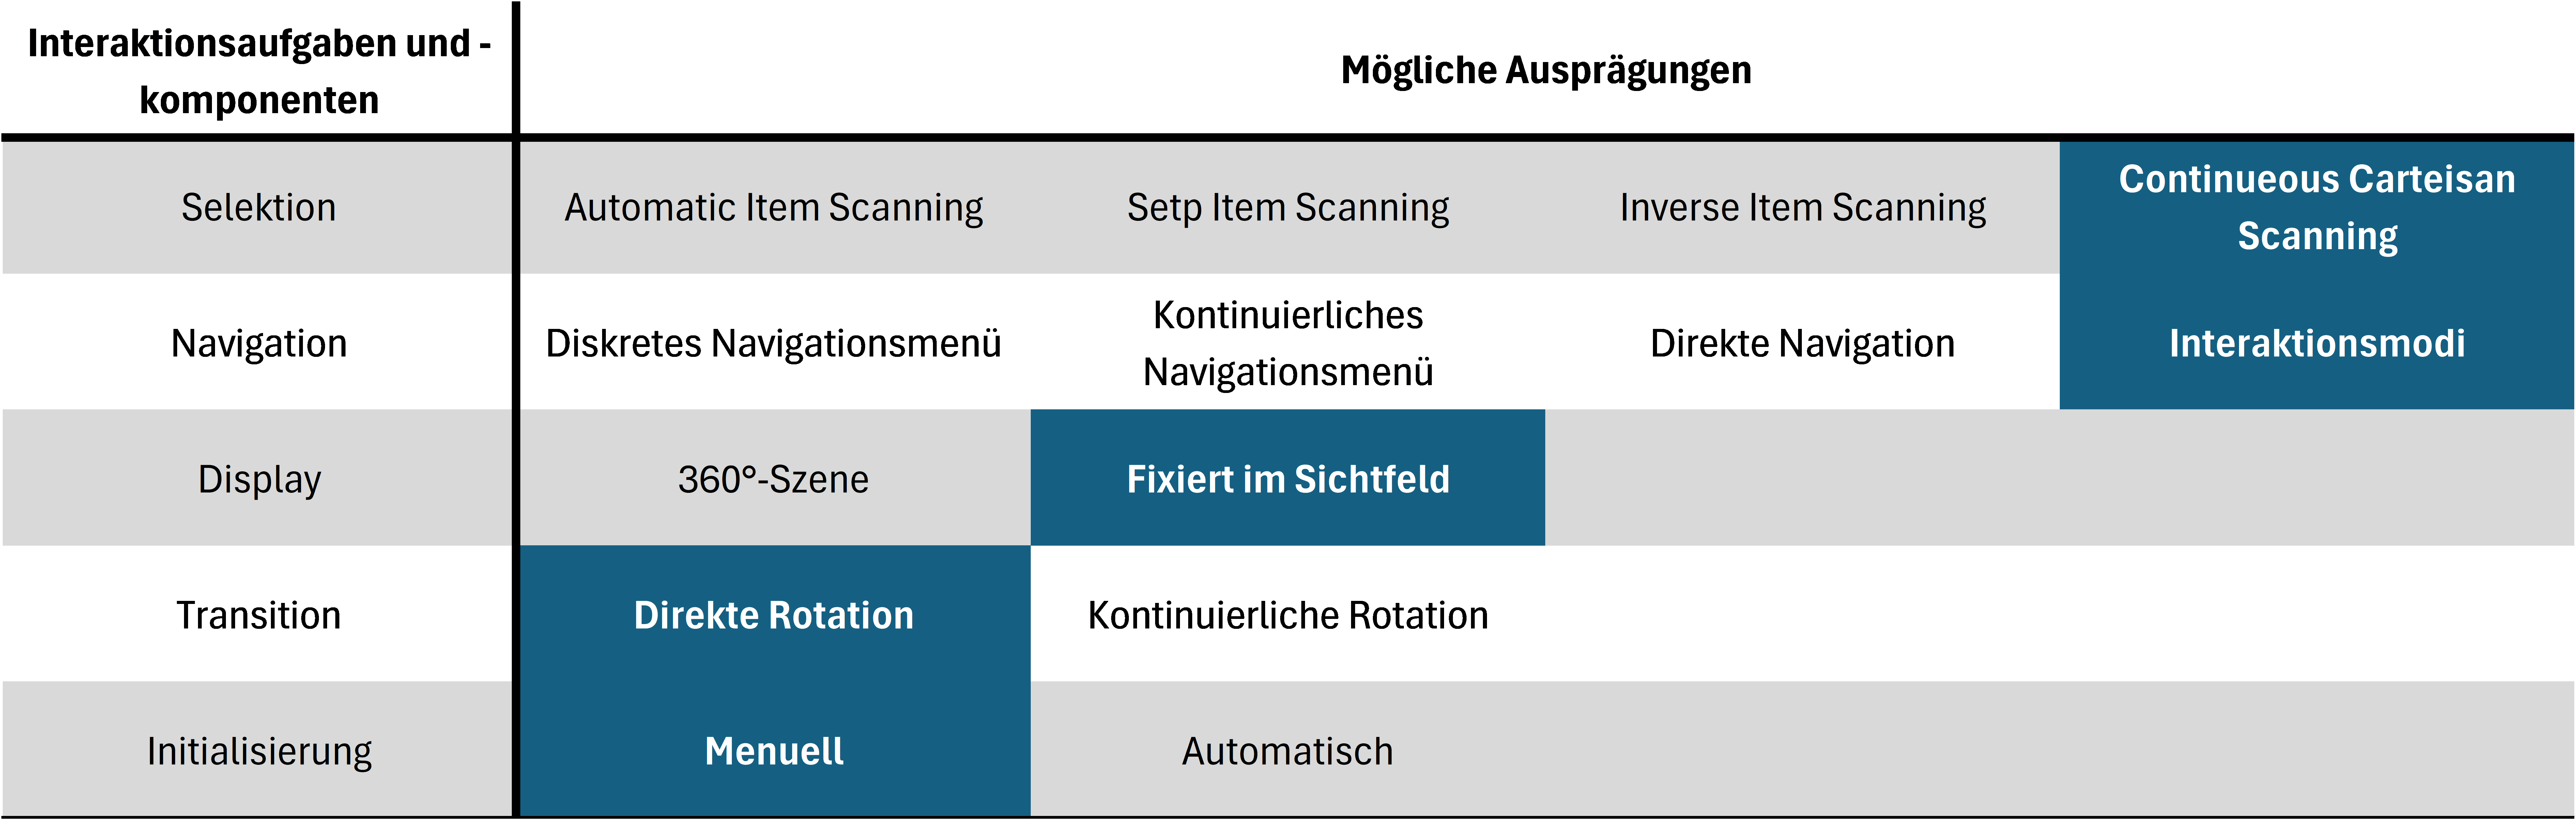
\includegraphics[width=0.95\textwidth]{images/MorphKasten-Cartesian.png}
    \caption{Darstellung des Konzept 2: Cartesian Scanning}
    \label{fig:MorphKasten-Cartesian}
\end{figure}

Das zweite Konzept basiert auf dem Continuous Cartesian Scanning. Die Bewertungen der Selektionsoptionen unterscheiden sich nicht wesentlich. Das Cartesian Scanning wurde bevorzugt vor dem Setp und Inverse Item Scanning ausgewählt, da es insbesondere hinsichtlich Komfort und Effizienz Vorteile aufweist. Für die Navigation werden Interaktionsmodi eingesetzt, da diese Option in den Bewertungen hinsichtlich Robustheit und auch Komfort leicht überlegen ist und eine klar strukturierte Interaktionsführung ermöglicht.
Der Wechsel zwischen den Modi erfolgt durch kurzes Halten des Schalters. Diese Methode hat den Vorteil, dass unbeabsichtigte Wechsel minimiert werden und gleichzeitig eine einfache Bedienung ermöglicht wird. Alternative Wechselmechanismen, wie ein doppeltes Drücken des Schalters oder die Integration eines zusätzlichen UI-Elements in die Szene, wurden verworfen, da sie entweder das Risiko unbeabsichtigter Eingaben erhöhen oder die visuelle Komplexität der Szene unnötig steigern würden.

Auch bei diesem Konzept wird das Scanning-Verfahren im Sichtfeld fixiert und die Transition erfolgt als diskrete Rotation, da diese Gestaltungsoptionen deutliche Vorteile gegenüber den anderen Optionen aufweisen. Die Initialisierung erfolgt auch hier manuell, um unbeabsichtigte Aktivierungen zu vermeiden und den Komfort zu erhöhen.

Die für dieses Konzept ausgewählten Gestaltungsoptionen der Interaktionsaufgaben und -komponenten sind in \autoref{fig:MorphKasten-Cartesian} zusammenfassend dargestellt.

Zur Optimierung des Cartesian Scanning werden unterschiedliche Farben für die Scan-Linien verwendet, um den aktiven Interaktionsmodus klar zu visualisieren. Zusätzlich ist das Scanning-Verfahren so gestaltet, dass die Linien nach ihrem ersten Durchlauf automatisch wieder von vorne beginnen, falls keine Eingabe erfolgt ist. Für den Fall, dass die erste Scan-Linie inkorrekt positioniert wurde, bietet das Verfahren die Möglichkeit, durch bewusstes mehrmaliges Durchlaufen der zweiten Scan-Linie den Scan abzubrechen und die Auswahl zurückzusetzen. Diese Maßnahmen dienen insbesondere der Steigerung der Robustheit.

{\normalfont \bfseries Zusammenfassung}

In diesem Kapitel wurde die Konzeption der Interaktionsmethoden durch eine systematische Analyse und Auswahl von Gestaltungsoptionen entlang definierter Parameter konkretisiert. Dabei wurden zwei Konzepte entwickelt, die auf den jeweiligen Stärken der analysierten Optionen aufbauen und durch gezielte Maßnahmen zur Kompensation möglicher Schwächen ergänzt werden. Während das erste Konzept auf dem Scanning-Verfahren Automatic Item Scanning basiert, wird für das zweite Konzept Continuous Cartesian Scanning als grundlegendes Interaktionsverfahren zur Selektion und Navigation gewählt. Im weiteren Verlauf der Arbeit werden die Konzepte als Vereinfachung über die verwendeten Scanning-Verfahren referenziert. 

Im folgenden \autoref{chap:Implementierung} wird die konkrete Umsetzung dieser Konzepte einschließlich der technischen Umsetzung der gewählten Gestaltungsoptionen sowie der definierten Kompensationsstrategien vorgestellt.
\chapter{Implementierung}

In diesem Kapitel wird die technische Umsetzung der erarbeiten Konzepte beschrieben. Dabei wird zunächst die grundlegende Architektur beschrieben, gefolgt von Grundlagen, die für beide Konzepte gleichermaßen entscheidend sind. Anschließend wird die spezifische Implementierung der beiden Konzepte tiefergehend vorgestellt. Hierbei wird zunächst das Item Scanning beschrieben und anschließend das Cartesain Scanning. Danach werden allgemeine Strategien zur Fehlerbehandlung sowie in der Entwicklung genutzte Debugging-Methoden vorgestellt. Abschließend werden Limitationen aufgezeigt und es wird ein kurzer Ausblick auf mögliche zukünftige Erweiterungen der Implementierung eröffnet. 

\section{Architektur}
Die für die Implementierung relevanten Erweiterungen im Rahmen dieser Arbeit wurden in der IngameScene vorgenommen. Nachfolgend sind die zentralen Komponenten dieser Szene aufgeführt, die für die Weiterentwicklung im Rahmen dieser Arbeit relevant waren. 

{\normalfont \bfseries Zentrale Komponenten der IngameScene}

\begin{itemize}
    \item \textit{Interaction Sphere:} Ein GameObject, an dem beim Laden einer neuen Szene alle interaktiven Paneo-Elemente als Child-Objekte angehängt werden.
    \item \textit{Scene Manager:} Enthält unter anderem das Script Scene Loader, das für das dynamische Laden der interaktiven Elemente verantwortlich ist. Dieses Script wurde zur Implementierung des Item Scanning erweitert. 
    \item \textit{XRRigMultiplayer:} Wird beim Start der Szene gespawnt und enthält unter anderem die Main Camera sowie den UI-Anchor. Dem UI-Anchor sind zentrale UI-Komponenten wie das Ingame-Menü und die Elemente für Nachrichten (Hint-Panel und Verify-Panel) untergeordnet.    
\end{itemize}

{\normalfont \bfseries Erweiterungen der ursprüglichen Szene im Rahmen dieser Arbeit}

Zur Implementierung der Scanning-Methoden wurden mehrere neue GameObjects und zugehörige Skripte in die IngameScene integriert. Diese werden folgend kurz aufgelistet und die wichtigsten Funktionalitäten vorgestellt. 

\begin{itemize}
    \item \textit{SwitchHandler:}
    Dieses Script verarbeitet die Eingaben des Nutzenden, die über das Unity Input System erfasst werden. Je nach gewählter Scanning-Methode (0 = Item Scanning, 1 = Cartesian Scanning) leitet der SwitchHandler die Eingaben an das entsprechende Script (FindAndHighlightButtons oder Cartesian Handler) weiter. Beim Cartesian Scanning überprüft der SwitchHandler zudem, ob der Schalter länger als zwei Sekunden gehalten wurde, um anschließend den Interaktionsmodus zu wechseln.
    \item \textit{FindAndHighlightButtons:}
    Hierbei handelt es sich um das zentrale Script für das Item Scanning. Es führt das schrittweise Hervorheben der interaktiven Elemente in der Szene aus und ermöglicht die Auswahl des aktuell hervorgehobenen Objekts.
    \item \textit{CartesianScanHandler:} 
    Dies ist das zentrale Script für das Cartesian Scanning. Es steuert, zu welchem Zeitpunkt die Animationen der Linien aufgerufen werden, berechnet den Schnittpunkt der Linien, überprüft, ob sich hinter dem Schnittpunkt ein interaktives Element befindet, und führt die Selektion oder einen Moduswechsel aus. 
    \item \textit{VisibleByCamera:}
    Dieses Script ist insbesondere für das Item Scanning relevant und prüft, ob sich ein interaktives Element im Sichtfeld der Kamera befindet.
    \item \textit{NextElementLine:} 
    Dieses Script dient der Visualisierung der Scanning-Reihenfolge im Item Scanning. Durch die hier gesteuerten Animationen wird verdeutlicht, welches Element als nächstes hervorgehoben wird, um die Reihenfolge für Nutzende nachvollziehbar zu gestalten.
    \item \textit{SoundHandler:}
    Dieses Script ist für die Steuerung der Feedback-Audioausgaben bei Interkationen zuständig.
\end{itemize}

Die aufgeführten Skripte kommunizierten größtenteils über direkte Methodenaufrufe miteinander, was eine schnelle und direkte Weiterleitung von Eingaben und Verarbeitungsergebnissen ermöglicht. Um die Übersichtlichkeit und Wartbarkeit des Codes sicherzustellen, wurden die Scanning-Verfahren so gestaltet, dass für jedes ein eigenes Hauptskript mit der wichtigsten Funktionalität erstellt wurde. Dadurch befindet sich die gesamte Logik für jedes Verfahren an einem zentralen Ort. Es ist somit nicht erforderlich, zwischen mehreren Skripten zu wechseln, um spezifische Funktionen zu finden und anzupassen oder zu erweitern. Dennoch wurden einige Funktionen bewusst ausgelagert. Die Prüfung, ob ein Objekt sichtbar im Blickfeld der Kamera ist, wurde in ein separates Skript überführt. So kann diese Prüfung gegebenenfalls unabhängig vom Scanning-Verfahren wiederverwendet werden. Die Methoden zur Animation der Linien im Cartesian Scanning wurden direkt an die animierten Objekte gebunden. Dies erleichtert die Konfiguration der Animationen und fördert eine klare Trennung der Verantwortlichkeiten. Für die Ausführung der Navigation wurden ebenfalls zusätzliche Skripte erstellt. Das Skript \textit{MenuNavigation} realisiert die Rotation des XRRigs beim Item Scanning, während das Skript \textit{ModeNavigation} diese Funktionalität für das Cartesain Scanning übernimmt. Die beiden Funktionalitäten wurden dabei bewusst auf zwei Skripte geteilt, um die Unabhängigkeit der beiden Scanning-Verfahren beizubehalten. 

\begin{figure}[tbh]
 \centering
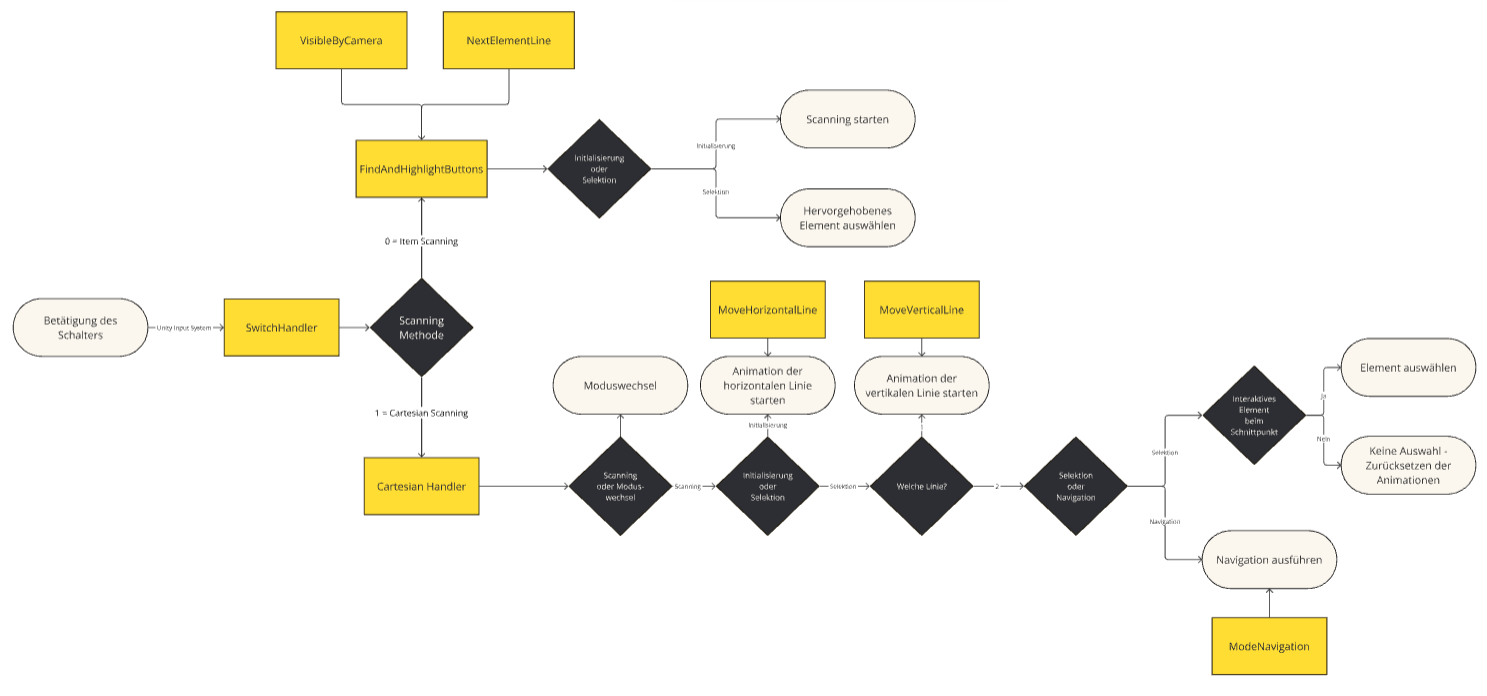
\includegraphics[width=1\textwidth]{images/FlussdiagrammArchitektur.png}
 \caption{Grundlegender Informationsfluss der Softwarearchitektur}
 \label{fig:infofluss}
\end{figure}

Der grundlegende Informationsfluss, der zwischen diesen vorgestellten Skripten besteht, wird in \autoref{fig:infofluss} veranschaulicht. Die Eingaben der Nutzenden werden über das Unity Input System erfasst und zunächst im \textit{SwitchHandler} verarbeitet. Abhängig von der gewählten Scanning-Methode wird die Eingabe an den entsprechenden Scanning Handler weitergeleitet. Beim Item Scanning übernimmt das Skript \textit{FindAndHighlightButtons} die schrittweise Hervorhebung der Elemente sowie die Selektion des aktuell hervorgehobenen Elements. Beim Cartesian Scanning steuert der \textit{CartesianScanHandler} die Animation der Linien, die Schnittpunktberechnung und die Auswahl der interaktiven Elemente.

\section {Gemeinsame Komponenten beider Konzepte}

Die Implementierung der beiden Scanning-Methoden basiert unter anderem auf gemeinsam genutzten Komponenten, die Funktionalitäten beider Verfahren unterstützen. Dazu gehören die Eingabeverarbeitung, die Audioausgabe sowie ein zusätzliches Highlight-GameObject, das allen interaktiven Objekten als Kindsobjekt hinzugefügt wird. 

{\normalfont \bfseries Eingabeverarbeitung}

Als Eingabe wurde zunächst eine neue Input Action erstellt, die die Leertaste der Tastatur als Simulation eines Scahlters verwendet. Diese Lösung ermöglicht eine einfache Simulation während der Entwicklung und Evaluation, wenn kein Schalter zur Verfügung steht. Für verschiedene Arten von Schaltern kann diese Konfiguration zukünftig leicht erweitert werden.

Für die Verarbeitung von Eingaben wurde das Skript \textit{SwitchHandler} als zentrale Komponente implementiert. Dieses nutzt die Events \textit{started} und \textit{canceled} des Unity Input System, um die Aktionen des Nutzenden zu erkennen und entsprechend zu verarbeiten. Bei der \textit{Started-Action} wird die Methode \textit{OnPressStarted} aufgerufen. In dieser wird der Zeitpunkt des Drückens zwischengespeichert und die Variable \textit{isPressing} wird auf \textit{true} gesetzt. Dies geschieht jedoch nur unter der Voraussetzung, dass das Cartesian Scanning als Scanning-Methode eingestellt ist. In der \textit{Update-Methode} wird daraufhin kontinuierlich überprüft, ob \textit{isPressing} auf \textit{true} steht und ob seit dem Beginn des Drückens bereits zwei Sekunden vergangen sind. Wenn dies der Fall ist, wird ein akustisches Feedback ausgelöst, das dem Nutzenden signalisiert, dass ein Wechsel des Interaktionsmodus bei Loslassen des Schalters durchgeführt wird.
Bei der \textit{Canceled-Action} wird die Methode \textit{OnPressEnded} aufgerufen. Hier wird zunächst geprüft, welche Scanning-Methode eingestellt ist. Ist das Item Scanning aktiv, wird die Eingabe an das \textit{FindAndHighlightButtons}-Skript weitergeleitet. Ist das Cartesian Scanning aktiv, wird zunächst die Dauer des Tastendrucks geprüft. Wurde die Taste länger als zwei Sekunden gedrückt, wird die Methode \textit{changeMode} im \textit{CartesianScanHandler} aufgerufen, um den Interaktionsmodus zu wechseln. Andernfalls wird die Methode \textit{Scanning} aufgerufen, um den Scanning-Vorgang zu starten. Die gewählte Scanning-Methode wird in einer Integer-Variable gespeichert, wobei 0 für das Item Scanning und 1 für das Cartesian Scanning steht. 

{\normalfont \bfseries Audioausgabe}

Die Anwendung bietet Nutzenden akustisches Feedback, das über den \textit{AudioHandler} realisiert wird. Dieser ermöglicht das Erzeugen einer AudioSource zur Laufzeit, die den übergebenen AudioClip abspielt und anschließend automatisch wieder entfernt wird. Diese Implementierung ist ressourcenschonend und verhindert Probleme, die auftreten könnten, wenn eine AudioSource an ein GameObject gebunden ist und dieses während der Laufzeit entfernt wird. Durch diese Lösung wird sichergestellt, dass alle Sounds vollständig abgespielt werden, was insbesondere für Benutzerfeedback von zentraler Bedeutung ist.

{\normalfont \bfseries Highlight Objekt}

Allen interaktiven Objekten wurde ein Highlight-Objekt als Child-Objekt hinzugefügt. Dieses Highlight besteht aus einer einfachen geometrischen Form (Sphere oder Cube), die mit einem transparenten Material versehen ist. Die Geometrie dient dazu, die Darstellung von Outlines zu ermöglichen, da diese nur an sichtbaren Meshes generiert werden können. Das Highlight-Objekt enthält zudem einen Mesh Renderer (initial deaktiviert), einen Collider und eine Outline, die mithilfe des kostenlosen Plugins Quick Outline aus dem Unity Asset Store realisiert wurde.
Das Highlight-Objekt wird von beiden Scanning-Methoden unterschiedlich genutzt. Beim Item Scanning wird die Outline durch Aktivieren des Mesh Renderers sichtbar gemacht, um zu visualisieren, dass dieses Objekt ausgewählt werden kann. Zusätzlich wird der Collider verwendet, um zu prüfen, ob das Objekt im Sichtfeld der Kamera liegt. Beim Cartesian Scanning wird der Collider ebenfalls verwendet. In diesem Zusammenhang jedoch um zu prüfen, ob hinter dem Schnittpunkt der Linien ein interaktives Objekt liegt. Auf die genaue Funktionsweise des Highlight-Objekts in den spezifischen Kontexten wird folgend in der Vorstellung der beiden Konzepte genauer eingegangen. 


\section{Scanning Methoden}

\subsection{Konzept 1 - Item Scanning }

Das Item Scanning basiert auf einer Liste, die alle interaktiven Elemente einer Szene enthält. Diese interaktiven Elemente (Interactables) werden beim Laden einer Szene durch das Skript \textit{SceneLoader} erzeugt und automatisch der Liste im Skript \textit{FindAndHighlightButtons} hinzugefügt. Zusätzlich werden zwei UI-Buttons hinzugefügt, die immer als HUD sichtbar sind. Dabei handelt es sich um einen Button zum Öffnen des Menüs und einen Button zum Öffnen des Navigationsmenüs. Sobald der \textit{SwitchHandler} eine Eingabe registriert, prüft er, ob das Scanning bereits aktiv ist oder initialisiert werden muss. Diese Information wird über einen Methodenaufruf an das Skript \textit{FindAndHighlightButtons} übergeben. Ist das Scanning noch nicht aktiv, wird die Methode \textit{StartItemScanning} aufgerufen, andernfalls die Methode \textit{SwitchSelection}. Diese beiden Methoden stellen die zentrale Funktionalität der Scanning-Methode dar. Im Folgenden werden diese und weitere relevante Aspekte näher beschrieben.

\textbf{Start und Verlauf des Scannings}

Die Methode \textit{StartItemScanning} startet eine Coroutine namens ItemScanning, in der der eigentliche Scan-Vorgang abläuft. Diese Coroutine iteriert über die Liste der interaktiven Elemente und hebt sie nacheinander hervor. Der Ablauf ist im folgenden Pseudocode \autoref{lst:codeItem} vereinfacht dargestellt.

\begin{lstlisting} [language=Python, caption=Vereinfachter Pseudocode des Item Scannings, label={lst:codeItem}]

IEnumerator ItemScanning()
{
    while (isScanActive)
    {
        foreach (GameObject button in allButtons)
        {
            // Versuche, das Highlight-Objekt zu finden
            GameObject highlight = button.transform.Find("Highlight").gameObject;
            
            if (highlight != null)
            {
                // Pruefe, ob das Highlight-Objekt sichtbar ist
                if (visibleByCamCheck.IsVisibleByCam(cam, highlight.GetComponent<Collider>()))
                {
                    // Aktiviere das Highlight-Objekt
                    highlight.GetComponent<MeshRenderer>().enabled = true;
                    highlightedObject = button;

                    // Starte die Animation zum naechsten Objekt
                    GameObject nextObject = GetNextHighlightableObject();
                    scriptNextElement.DrawLineBetweenElements(highlightedObject, nextObject);

                    // Warte fuer die Scan-Rate
                    yield return new WaitForSeconds(ScanRate);

                    // Deaktiviere das Highlight-Objekt, falls es noch existiert
                    if (highlight != null)
                    {
                        highlight.GetComponent<MeshRenderer>().enabled = false;
                    }
                }
            }
        }
    }
}

\end{lstlisting}

Die Iteration läuft, solange das Scanning aktiv ist. Für das aktuelle Objekt wird zunächst geprüft, ob es ein Highlight-GameObject als Kind-Objekt enthält. Diese Prüfung stellt sicher, dass wirklich nur Objekte in den Scan-Vorgang einbezogen werden, die auch visuell hervorgehoben werden sollen. Ist ein Highlight-Objekt vorhanden, wird über den Collider des Objekts ermittelt, ob es sich aktuell im Sichtfeld der Kamera befindet. Dies geschieht über das Skript \textit{VisibleByCamera}.
Ist diese Prüfung positiv, wird das Highlight durch Einschalten des Mesh Renderers aktiviert. Gleichzeitig wird das hervorgehobene Objekt in einer entsprechenden Variablen gespeichert, um bei der Selektion darauf zugreifen zu können. Anschließend wird das nächste hervorzuhebende Objekt bestimmt und eine Animation gestartet, die eine Linie zwischen dem aktuellen und dem nächsten Objekt visualisiert. Diese Animation wird weiter unten ausführlicher behandelt. Nach Ablauf der Wartezeit, die durch die Scan Rate bestimmt wird, wird der Mesh Renderer des Highlight-Objektes wieder deaktiviert, sofern das Objekt noch existiert. Dies ist notwendig, da das Objekt unter Umständen während der Wartezeit gelöscht werden kann. Würde an dieser Stelle keine erneute Überprüfung erfolgen, käme es zu einer NullPointerException.


\textbf{Auswahl eines interaktiven Elements}

Die Auswahl eines hervorgehobenen Elements erfolgt über die Methode SwitchSelection. Hier wird geprüft, ob ein Objekt aktuell hervorgehoben ist. Ist dies der Fall, wird die Button-Komponente des Objekts gesucht und deren OnClick-Event ausgelöst. Der Ablauf ist im folgenden Pseudocode \autoref{lst:selectItem} veranschaulicht.

\begin{lstlisting} [language=Python, caption=Vereinfachter Pseudocode der Selektion des Item Scanning, label={lst:selectItem}]

public void SwitchSelection()
{
    if (highlightedObject != null)
    {
        // Suche nach der Button-Komponente
        GameObject buttonTrigger = highlightedObject.transform.Find("Btn_Trigger").gameObject;
        Button buttonToClick = buttonTrigger.GetComponent<Button>();

        // Loese das OnClick-Event aus
        if (buttonToClick != null)
        {
            ExecuteEvents.Execute(
                buttonToClick.gameObject,
                new BaseEventData(EventSystem.current),
                ExecuteEvents.submitHandler
            );
        }
    }
}
    
\end{lstlisting}

Die gleiche Logik wird für die Navigation verwendet. Wenn ein Pfeilbutton im Navigationsmenü ausgewählt wird, wird das OnClick-Event des Buttons ausgelöst, welches wiederum die Methode turnLeft bzw. turnRight im Skript MenuNavigation aufruft. Diese Methoden drehen das XRRig um 40° (rechts) bzw. -40° (links).

\textbf{Animation zwischen dem aktuellen und folgenden Element}

Um die Reihenfolge zu verdeutlichen, in der die interaktiven Objekte hervorgehoben werden, wird eine Linie zwischen dem aktuellen und dem nächsten Element gezogen. Dazu wurde der \textit{IngameScene} das GameObject \textit{NextElementLine} hinzugefügt. Dieses enthält einen Line Renderer zur Darstellung der Linie sowie das Skript \textit{NextElementLine}, das die Steuerung der Animation übernimmt.
Die Animation wird als Coroutine umgesetzt. Der Startpunkt der Linie ist die Position des aktuell hervorgehobenen Elements, der Endpunkt die Position des nächsten Elements. Die Sichtbarkeit der Linie wird über die AlphaKeys des Line Renderers gesteuert, die von 0 auf 1 gesetzt werden. Dadurch wird die Linie schrittweise sichtbar. Die Animationsdauer entspricht der Scan Rate. Damit die Linie die Position dynamischer UI-Elemente korrekt darstellt, werden Start- und Endpunkte in der Update-Methode jeden Frame aktualisiert.

\textbf{Herausforderungen}

Die Herausforderungen bei der Implementierung des Item Scanning lagen insbesondere in der Unterscheidung der verschiedenen Ebenen. Wird z.B. ein Menü oder ein Dialogfeld geöffnet, so muss das Scanning auf diese Teilauswahl von Items beschränkt werden. Die Lösung dieses Problems wird im Folgenden exemplarisch an einem Dialog-Interactable beschrieben. 
Wird das Dialog-Objekt innerhalb des ItemScanning ausgewählt, wird das OnClick-Ereignis ausgelöst. Dadurch wird die Methode DialogScan aufgerufen. Dieser Methode werden beim Aufruf die Buttons der Antwortoptionen übergeben. Aus diesen Optionen wird ein Array erstellt, das dann mit der oben beschriebenen Logik durchlaufen werden kann. Die Auswahloptionen müssen also dynamisch angepasst werden, je nachdem welches Objekt aktiv ist bzw. sich auf der vordersten Ebene befindet. Dies erfordert besondere Aufmerksamkeit bei der Implementierung, da verschiedene Fälle berücksichtigt werden müssen. Für jedes Objekt, das eine weitere Ebene öffnet, muss geprüft werden, wie sich die Auswahl der Scan-Optionen dadurch ändert. 

\subsection{Konzept 2 - Cartesian Scanning}

Um das Cartesian Scanning zu implementieren, wurden zwei neue GameObjects erstellt und der Kamera im XRRig untergeordnet. Diese GameObjects enthalten jeweils ein Canvas, das annähernd auf die Größe des Sichtfeldes skaliert ist. Auf diesem Canvas befindet sich wiederum ein GameObject mit einer Rect Transform-Komponente, einem Line Renderer zur Darstellung der Linien sowie dem Skript \textit{MoveHorizontalLine} bzw. \textit{MoveVerticalLine}. Die GameObjects sind zu Beginn der Anwendung deaktiviert und werden erst während des Scan-Vorgangs aktiviert.
Die horizontale Linie bewegt sich von oben nach unten vor dem Nutzenden, während die vertikale Linie sich von links nach rechts bewegt. Die Bewegung der Linien wird über die genannten Skripte gesteuert. Der Aufbau dieser Skripte wird im Folgenden näher beschrieben. 

\textbf{Animation der Linien}

Die Methode \textit{StartAnimation} startet die Coroutine \textit{MoveLine}, in der die Bewegung der Linie gesteuert wird. Hier wird zunächst die Start- und Endposition der Linie definiert. Bei der horizontalen Linie sind dies der obere und der untere Rand des Canvas. Bei der vertikalen Linie entspricht dies dem linken und rechten Rand des Canvas. Nachfolgend ist in \autoref{lst:moveLine} ein Ausschnitt aus dieser Coroutine zur Veranschaulichung der Bewegung dargestellt. 

\begin{lstlisting} [language=Python, caption=Ausschnitt aus der Methode zur Animation der Linien im Cartesian Scanning, label={lst:moveLine}]

while (currentTime <= scanRate)
{
    currentTime += Time.deltaTime;
    normalizedValue = currentTime / scanRate;
    rectTransform.anchoredPosition = Vector3.Lerp(startPosition, endPosition, normalizedValue);
    yield return null;
}
\end{lstlisting}

Sobald die Linie ihre Endposition erreicht hat, wird über eine Zählervariable geprüft, ob die Animation bereits dreimal hintereinander ausgeführt wurde. Ist die Linie noch nicht dreimal durchgelaufen, wird die Animation zurückgesetzt und erneut gestartet. Erst nach dem dritten Durchlauf wird die Reset-Methode im CartesianScanHandler aufgerufen, wo der gesamte Fortschritt des Scanning zurückgesetzt wird. Dieses wiederholte Durchlaufen wurde zur Fehlerkorrektur implementiert. Wird die gewünschte Position der Linie beim ersten Durchlauf verfehlt, kann einfach abgewartet werden, bis die Linie wieder die gewünschte Position erreicht hat. Durch den Abbruch nach drei Durchläufen werden zudem vermeidbare Fehlauswahlen vermieden.

Eine weitere wesentliche Methode innerhalb des Skripts ist \textit{StopAnimation}. Diese bewirkt, dass die aktuell laufende Coroutine gestoppt wird, sodass die Linie in ihrer aktuellen Position verbleibt. Die Methode wird aufgerufen, sobald Nutzende die Position der Linie im Zuge des Scanning setzen möchten.

\textbf{Steuerung des Scanning-Prozesses}

Die eigentliche Steuerung des Cartesian Scanning erfolgt im Skript \textit{CartesianScanHandler}. Wird im \textit{SwitchHandler} eine Eingabe registriert, wird die Methode Scanning im \textit{CartesianScanHandler} aufgerufen. Diese prüft, in welchem Stadium sich der Scanning-Prozess befindet, und ruft entsprechend die nächste erforderliche Methode auf (vgl. \autoref{lst:scanningCartesian}). 

\begin{lstlisting} [language=Python, caption=Methode Scanning im CartesianScanHandler, label={lst:scanningCartesian}]

public void Scanning()
{
    if (!firstStarted)
    {
        ScanningFirstLine();
    }
    else
    {
        if (!secondStarted)
        {
            StopFirstLine();
        }
        else
        {
            Selection();
        }
    }
}
    
\end{lstlisting}

Die Methode \textit{ScanningFirstLine} aktiviert das GameObject der horizontalen Linie und ruft die Methode \textit{StartAnimation} im Skript \textit{MoveHorizontalLine} auf. In der Methode \textit{StopFirstLine} wird diese durch den Methodenaufruf \textit{StopAnimation} gestoppt, das GameObject der vertikalen Linie aktiviert und die Animation gestartet. In der Methode \textit{Selection} wird anschließend die Animation der zweiten Linie gestoppt, die beiden GameObjects wieder deaktiviert, die Animationen zurückgesetzt und die Variablen \textit{firstStarted} und \textit{secondStarted} wieder auf false gesetzt. Um die Selektion durchzuführen, wird die Methode \textit{FindIntersection} aufgerufen. Hier wird der Schnittpunkt der Linien berechnet. Dies wird im Folgenden anhand von Pseudocode veranschaulicht. 

\begin{lstlisting} [language=Python, caption=Pseudocode zur Veranschaulichung der Methode FindIntersection im CartesianScanHandler, label={lst:scanningCartesian}]

    public void FindIntersection()
    {
        // Positionen der Linien im Canvas Space
        Vector2 horizontalLinePosition = horizontalLine.anchoredPosition;
        Vector2 verticalLinePosition = verticalLine.anchoredPosition;
        
        // Berechnung Schnittpunkts Canvas Space
        Vector2 intersectionInCanvasSpace = new Vector2(verticalLinePosition.x, horizontalLinePosition.y );
        
        // Umwandlung in Weltkoordinaten
        Vector3 intersectionWorldPosition = horizontalLine.transform.parent.TransformPoint(intersectionInCanvasSpace);

        // Selektionsmodus ist aktiv
        if (!navModeActive)
	    {
            CheckForInteractiveElement(intersectionWorldPosition);
        }
        // Navigationsmodus ist aktiviert
        else
        {
            modeNav.turn(intersectionWorldPosition);
        }
    }

\end{lstlisting}

Je nachdem, welcher Modus aktiv ist, wird anschließend unterschiedlich verfahren. Ist der Selektionsmodus aktiviert, wird mit Hilfe der Methode \textit{CheckForInteractiveElement} überprüft, ob sich hinter dem Schnittpunkt der Linien ein interaktives Objekt befindet. Dazu wird mittels eines SphereCasts ein Ray von der Kameraposition durch den berechneten Schnittpunkt erzeugt. An dieser Stelle wurde ein SphereCast anstelle eines einfachen Rays gewählt, um einen Toleranzbereich in Form eines Radius einführen zu können. Dadurch wird ein Objekt auch dann ausgewählt, wenn der Schnittpunkt das Objekt knapp verfehlt. Es wird geprüft, ob dieser Ray den Collider eines Highlight-Objektes getroffen hat. Ist dies der Fall, wird wie beim Item Scanning das OnClick-Event der Button-Komponente des entsprechenden Objekts ausgelöst. Trifft der Ray auf mehrere Objekte, z.B. wenn zwei Ebenen mit interaktiven Elementen übereinander liegen, wird stets das Objekt ausgewählt, auf das der Ray zuerst trifft. Das heißt, es wird das Element ausgewählt, das näher an der Kamera positioniert ist. Dadurch wird sichergestellt, dass UI-Elemente wie das Ingame-Menü oder das Hint-Panel bevorzugt ausgewählt werden und keine unbeabsichtigten Selektionen bei Verdeckungen auftreten. Wurde kein Objekt getroffen, wird lediglich ein Audio-Feedback ausgelöst. 

Im Navigationsmodus hingegen wird die Methode \textit{turn} im Skript ModeNavigation aufgerufen. Hier wird die y-Koordinate des Schnittpunkts genutzt, um die Rotation des XRRigs entsprechend anzupassen.

\textbf{Wechsel zwischen Selektions- und Navigationsmodus}

Wird im \textit{SwitchHandler} registriert, dass der Schalter länger als 2 Sekunden gehalten wurde, wird die Methode \textit{changeMode} im \textit{CartesainScanHandler} aufgerufen. In dieser Methode wird die boolesche Variable \textit{navModeActive} entsprechend geändert. War diese zuvor auf true, so wird sie nun auf false gesetzt und umgekehrt. Außerdem wird die Farbe der Linie Renderer angepasst. Ist der Navigationsmodus aktiv, werden die Linien blau dargestellt, ist der Selektionsmodus aktiv, werden die Linien pink dargestellt. Dies dient dazu, den Nutzenden eine visuelle Rückmeldung darüber zu geben, welcher Modus gerade aktiv ist. Bei der Auswahl der Farben wurde darauf geachtet, dass diese einen relativ hohen Kontrast aufweisen, damit der Unterschied möglichst auch für Menschen mit Farbschwäche wahrnehmbar ist. 

\textbf{Herausforderungen}

Die Implementierung des Cartesian Scanning war insgesamt aufwendiger als die Implementierung des Item Scanning. Es werden mehr Objekte und Skripte benötigt, um das Scanning zu realisieren. Ist das Grundprinzip jedoch einmal implementiert, ist es vergleichsweise robust. Ein Vorteil dieses Verfahrens liegt insbesondere darin, dass Objekte auf unterschiedlichen Ebenen nicht separat betrachtet werden müssen. Dadurch kann die Implementierung insgesamt einfacher um neue Interaktionselemente erweitert werden. 
Eine Herausforderung bei der Implementierung war die Berechnung des korrekten Schnittpunktes sowie die Festlegung eines geeigneten Radius für den SphereCast. Bei der Berechnung des Schnittpunktes musste berücksichtigt werden, dass sich die Linien auf einem Canvas befinden und somit ihre Position in Abhängigkeit von diesem bestimmt wird. Um die tatsächliche Position in Weltkoordinaten zu erhalten, muss zunächst eine Umrechnung erfolgen. Die Festlegung des Radius des SphereCasts stellte eine Herausforderung dar, da hier ein Kompromiss gefunden werden musste. Der Radius musste groß genug sein, um kleine Verfehlungen zu tolerieren, aber klein genug, um bei dicht beieinanderliegenden Objekten eine korrekte Auswahl zu ermöglichen. Es galt also, verschiedene Werte auszuprobieren und zu prüfen, ob sich das gewünschte Ergebnis einstellt. 

\section{Strategien zur Fehlervermeidung und Debugging}

Um Fehlermeldungen vorzubeugen und die Anwendung robuster zu gestalten, wurde an vielen Stellen im Code mit try and catch Abfragen gearbeitet. Insbesondere NullPointerExceptions werden so abgefangen. Dies wird z.B. beim Item Scanning verwendet. Wenn bspw. ein Objekt kein Highlight-Objekt hat oder das Objekt zur Laufzeit der Coroutine gelöscht wird, wird dies abgefangen und das Objekt kann problemlos übersprungen werden. Des Weiteren wurde viel mit boolschen Variablen gearbeitet, um die Abläufe besser verfolgen und steuern zu können. So wird z.B. verhindert, dass zwei Item Scanning Prozesse gleichzeitig gestartet werden. Beim Cartesian Scanning geben die Funktionen bei der Selektion, also CheckForInteractiveElement und modeNav.turn, boolsche Werte zurück, die eine Rückmeldung darüber liefern, ob die Ausführung erfolgreich war. So können die verschiedenen Ausgänge mit unterschiedlichem Audio-Feedback kommuniziert werden. 

Für das Debugging wurde insbesondere die Debug-Klasse von Unity verwendet. An mehreren Stellen wurden Debug.Logs eingefügt, um den Ablauf besser nachvollziehen zu können und schneller zu erkennen, an welcher Stelle im Code Fehler auftreten. Für das Cartesian Scanning wurden zusätzlich einzelne Schritte visuell veranschaulicht. So wurde bspw. während der Entwicklung ein Testobjekt in Form eines einfachen Würfels an die Position des berechneten Schnittpunktes gelegt, um leichter überprüfen zu können, ob dieser korrekt berechnet wird. Ebenso wurde der SphereCast mittels Debug.DrawRay visualisiert, um in der Scene View überprüfen zu können, ob dieser korrekt gezeichnet wird.


\section{Limitationen und mögliche Erweiterungen}

Da die vorliegende Arbeit eine prototypische Implementierung umfasst, bestehen noch mehrere Limitationen, die zukünftige Weiterentwicklungen erforderlich machen.
Eine zentrale Einschränkung beim Item Scanning liegt in der fehlenden Konfigurierbarkeit der Reihenfolge, in der interaktive Objekte hervorgehoben werden. Gegenwärtig basiert die Reihenfolge auf der Reihenfolge, in der die Objekte beim Laden der Szene erzeugt werden. Dies kann dazu führen, dass in der Szene räumlich nahe beieinander liegende Objekte nicht nacheinander hervorgehoben werden, was von Nutzenden als nicht erwartungskonform wahrgenommen werden könnte. Um dieses Problem zu beheben, könnte ein Parameter „Position im Scanning“ in die Prefabs der interaktiven Objekte integriert werden. Durch eine Sortierung der Liste der interaktiven Objekte anhand dieses Parameters könnte die Reihenfolge an die räumliche Anordnung angepasst werden.Im Rahmen dieser Arbeit wurde diese Option nicht implementiert, da kein Zugriff auf den Webeditor von PaneoVR besteht und somit dieser Parameter nicht in den Webeditor und damit nicht in die Gestaltung von Szenarien integriert werden konnte. 

Eine weitere Limitation betrifft die Konfigurierbarkeit der Scan Rate und des Scanning-Verfahrens. Diese Einstellungen können derzeit nur über den Unity-Editor angepasst werden, sodass die Nutzenden keine Möglichkeit haben, diese direkt innerhalb der Anwendung zu ändern. Diese Einschränkung wurde bewusst in Kauf genommen, um die Durchführung der Evaluation zu vereinfachen und vergleichbare Ergebnisse zu gewährleisten. Dies wird im Kapitel Evaluation ausführlicher erläutert. 
Für den späteren produktiven Einsatz der Scanning-Verfahren wäre jedoch eine entsprechende Anpassungsoption notwendig, um die individuellen Präferenzen und Bedürfnisse der Nutzenden berücksichtigen zu können.

Beim Catesian Scanning stellt die Platzierung der Linien auf einem an das Sichtfeld der Nutzenden angepassten Canvas eine mögliche Einschränkung dar. Für einige Nutzende könnte dies möglicherweise nicht optimal sein. Zukünftige Entwicklungen könnten hier Anpassungsoptionen für den Scanbereich vorsehen, um die Benutzerfreundlichkeit zu erhöhen. Eine weitere Einschränkung liegt in der planaren Darstellung der Linien auf einer Ebene. Es wäre sinnvoll zu untersuchen, ob eine sphärische Darstellung, die sich an der Sphäre des 360-Grad-Videos orientiert, die Interaktion noch natürlicher gestalten und die Präzision erhöhen könnte.

Außerdem könnte getestet werden, ob ein multimodales Feedback das Cartesian Scanning noch unterstützen könnte. Beim Item Scanning wurde beispielsweise ein Audiosignal hinzugefügt, das jedes Mal ertönt, wenn ein neues Objekt hervorgehoben wird. Ein ähnliches Prinzip könnte beim Cartesian Scanning eingeführt werden. Hier könnte bspw. ein Audiosignal ertönen, wenn eine Linie während der Aniamtion mit einem interaktiven Objekt kollidiert. 

\section{Installation, Nutzerdokumentation}

Unbedingt zur Implementierung gehört dann am Ende auch eine Beschreibung, wie man die Implementierung zu nutzen hat. Dazu gehört die Beschreibung, wie man die Implementierung bezieht und installiert, genauso wie eine kurze Beschreibung der Bedienung. Falls letztere zu umfangreich werden würde, aber notwendig ist, kann diese auch im Anhang aufgeführt und mit einem Verweis gearbeitet werden.

\chapter{Evaluation}
\label{chap:Evaluation}
% TO DO: Abbildungen optimieren, ggf. Abkürzungen für die statistischen Sachen 

Die Evaluation der entwickelten Interaktionsschnittstellen erfolgt in zwei Hauptabschnitten: einer technischen und einer inhaltsbasierten Evaluation. Ziel ist es, sowohl die technische Leistungsfähigkeit der Schnittstellen als auch deren Wechselwirkung mit den Inhalten zu analysieren. Im folgenden wird zunächst die technische Evaluation gefolgt von der inhaltsbasierten Evaluation beschrieben. Anschließend wird die Durchführung der Evaluation geschildert und die Ergebnisse werden vorgestellt. 

\section{Konzeption der Evaluation}

\subsection{Technische Evaluation}

Der technische Abschnitt der Evaluation dient insbesondere der Überprüfung der Annahmen zu technischen Parametern wie Geschwindigkeit, Effizienz, Robustheit und Erlernbarkeit, die im Rahmen der Konzeption getroffen wurden. Darüber hinaus soll die gründsätzliche Usability der Schnittstellen evaluiert werden. Für jede Schnittstelle wird ein spezifisches Szenario entwickelt, in dem die technischen Fähigkeiten der Schnittstellen in möglichst anspruchsvollen Situationen getestet werden. Die Szenarien sind in Bezug auf die verwendeten Elemente und die Anzahl der durchzuführenden Eingaben vergleichbar. Beide Szenarien bestehen aus zwei Abschnitten. Im ersten Abschnitt steht die einfache Selektion von Objekten im Vordergrund. Im zweiten Abschnitt hingegen liegt der Schwerpunkt auf der Interaktion mit Dialogfeldern und damit auf der Interaktion auf verschiedenen Ebenen sowie auf der Selektion von Objekten, die räumlich nahe beieinander liegen. Ziel dieses Aufbaus ist es, möglichst viele Interaktionen zu generieren, um eine breite Datengrundlage zu erhalten. Darüber hinaus ermöglicht das Design die Beobachtung möglicher Lerneffekte bei den Testpersonen. Die Anordnung der Elemente innerhalb der Szenen ist absichtlich herausfordernd gestaltet, um insbesondere die Robustheit und Effektivität der Schnittstellen zu erproben. Darüber hinaus sind die Elemente über die gesamte 360°-Szene verteilt, um die Nutzung der Navigation zu forcieren. Im Folgenden werden die Herausforderungen, die bei der Anordnung der Elemente innerhalb der Szene berücksichtigt wurden, im Detail dargestellt. 

\textbf{Herausforderungen der implementierten Interaktionsschnittstellen}

Als Herausforderung bei der Verwendung von Item Scanning wird zunächst eine hohe Anzahl von Elementen in der Szene betrachtet, deren Reihenfolge im Scanning nicht unmittelbar ersichtlich ist. Dies erfordert ein aktives und konzentriertes Verfolgen der Reihenfolge, um das gewünschte Element auswählen zu können. Darüber hinaus wird die Positionierung von Elementen am Rand des Sichtfeldes als Herausforderung angesehen. Diese Elemente könnten von den Nutzenden leicht übersehen oder in der Scan-Reihenfolge nicht erwartet werden, was zu fehlerhaften oder unbeabsichtigten Selektionen führen könnte. Darüber hinaus stellen längere Wartezeiten für Elemente, die erst spät in der Scanning-Reihenfolge erscheinen, eine weitere potenzielle Herausforderung dar. Diese könnten zu Ungeduld und damit zu fehlerhaften Eingaben führen. Auch die Interaktion auf mehreren Ebenen, z. B.  das Schließen von Pop-Ups oder das Navigieren in Dialogfeldern, wird als weitere Herausforderung angesehen.

Im Gegensatz dazu ist beim Cartesian Scanning vermutlich die größte Herausforderung, das gewünschte Element bei nahe beieinander liegenden Elementen auszuwählen. Je näher die Elemente beieinander liegen, desto präziser muss die Selektion erfolgen. Dies erfordert dementsprechend ein genaues Timing und eine hohe Konzentration. Darüber hinaus könnte auch bei diesem Scanning-Verfahren die Positionierung von Elementen am Rand des Sichtfeldes als Herausforderung darstellen. Insbesondere wenn sich Objekte weit oben oder weit links befinden, kann es schnell passieren, dass Nutzende die Selektion verpassen und auf einen weiteren Durchlauf der Scan-Linie warten müssen. Als letzte Herausforderung wird die Interaktion auf mehreren Ebenen gesehen. Insbesondere bei beweglichen Pop-Ups oder Menüs, die sich mit der Kopfposition im Sichtfeld bewegen, könnte es schnell zu Verschiebungen und damit zu Fehleingaben kommen. Auch hier ist somit eine erhöhte Konzentration erforderlich. 

Die Szenarien für den technischen Abschnitt der Evaluation werden so gestaltet, dass diese Herausforderungen gezielt getestet werden. Während im ersten Abschnitt die Positionierung der Elemente im Vordergrund steht, werden im zweiten Abschnitt die Nähe und die Ebenenstruktur der Objekte aufgegriffen. Zur Minimierung von Zufallseffekten wurde eine Mindestanzahl von fünf gleichartigen Objekten pro Szenario integriert. \autoref{Anhang:screenTechnisch} beinhaltet Abbildungen der erstellten Szenarien. 

\textbf{Fragestellungen und Datenerhebnung}

Durch die Datenerhebnung im technischen Abschnitt sollen insbesondere folgende Fragestellungen zu den genannten Parametern beantwortet werden können:

\textit{Geschwindigkeit} 
    \begin{itemize}
        \item Wie lange dauert es, das Szenario zu durchlaufen? Begünstigt eine Schnittstelle einen schnelleren Durchlauf?
        \item Wie lang ist die Interaktionsgeschwindigkeit bei den Schnittstellen? Bietet eine Schnittstelle eine deutlich schnellere Interaktionsgeschwindigkeit?
        \item Gibt es Faktoren, die die Interaktionsgeschwindigkeit beeinflussen, etwa die Position der Objekte im Sichtfeld?
        \item Gibt es beim Cartesian Scanning deutliche Unterschiede in der Interaktionsgeschwindigkeit abhängig von der Position der Objekte?
        \item Führt eine schnellere Interaktionsgeschwindigkeit zu einer besseren Bewertung der Usability? 
    \end{itemize}
\textit{Robustheit}
    \begin{itemize}
        \item  Wie häufig treten Fehler bzw. unbeabsichtigte Eingaben bei den jeweiligen Schnittstellen auf? 
        \item Was sind die Gründe für auftretende Fehler?
        \item Wie häufig werden zwei oder mehr Durchgänge im Scanning benötigt?
        \item Wie häufig werden beim Cartesian Scanning leere Eingaben zur Korrektur von Fehlen verwendet? 
    \end{itemize}
\textit{Erlernbarkeit}
    \begin{itemize}
        \item Zeigt sich im Verlauf des Szenarios ein deutlicher Lerneffekt? 
        \item Wie entwickelt sich die Interaktionsgeschwindigkeit im Verlauf des Szenarios? 
        \item Reduziert sich die Anzahl der Fehler mit zunehmender Erfahrung?
    \end{itemize}
\textit{Usability}
    \begin{itemize}
    \item Wie wird die Usability der Schnittstellen bewertet?
    \item Gibt es deutliche Unterschiede in der Bewertung der Usability zwischen den beiden Schnittstellen? 
    \end{itemize}

Die Erfassung der technischen Daten erfolgt durch die Kombination von automatischem Logging direkt aus Unity und einem Evaluationsprotokoll (siehe \autoref{Anhang:protokoll}). Es wird für jede durchgeführte Selektion die Interaktionsgeschwindigkeit ausgegeben. Außerdem wird die benötigte Zeit von Start bis Abschluss des Szenarios gespeichert. Fehler werden manuell gezählt und kategorisiert und zusätzliche Beobachtungen dokumentiert. Zur Evaluation der Usability wird die SUS in digitaler Form verwendet.

\textbf{Erwartete Ergebnisse der technischen Evaluation}

Die Erwartungen an die Ergebnisse der technischen Evaluation der Schnittstellen basieren auf den theoretischen Überlegungen, die im Rahmen der Konzeption aufgestellt wurden (vgl. \autoref{subchap:EinordnungNachParameter}). Es wird erwartet, dass das Item Scanning intuitiver und schneller erlernbar ist als das Cartesian Scanning. Außerdem wird erwartet, dass Item Scanning robuster ist, was sich in einer geringeren Anzahl von Fehlern in der Anwendung widerspiegelt. Beim Cartesian Scanning können insbesondere nah beieinander liegende Objekte oder Objekte am Rand des Sichtfeldes eine höhere Fehlerquote begünstigen. Auch hinsichtlich der Interaktionsgeschwindigkeit wird eine leichte Überlegenheit des Item Scanning erwartet.
Gleichzeitig wird angenommen, dass das Item Scanning bei der Navigation insgesamt etwas langsamer ist, da mehrere Eingaben zum Erreichen eines größeren Rotationswinkels erforderlich sind. Das Cartesian Scanning hingegen ermöglicht eine effizientere Navigation und deckt größere Rotationswinkel schneller ab. Generell wird erwartet, dass das Item Scanning zu besseren technischen Ergebnissen führt.

\subsection{Inhaltsbasierte Evaluation}

Der zweite Abschnitt der Evaluation widmet sich der Wechselwirkung zwischen Interaktionsschnittstelle und Inhalt. Hier stehen die Parameter Komfort und Effizienz im Vordergrund . Darüber hinaus wird die UX der Schnittstellen betrachtet. Die inhaltsbasierte Evaluation ergänzt den technischen Abschnitt, indem die Schnittstellen in realistischeren Anwendungsszenarien getestet werden.
Es werden zwei Szenarien in Form einfacher Rätsel nach dem Prinzip von \textit{Escape Rooms} erstellt. Die Aufgabe der Testpersonen besteht darin, einen hinter interaktiven Objekten wie Bildern oder Audiodateien versteckten Zahlencode zu ermitteln bzw. einen Schlüssel zur Lösung des Szenarios zu finden. Die Rätsel sind bewusst einfach gehalten, um die kognitiven Fähigkeiten der Testpersonen außerhalb der Verwendung der Schnittstellen nicht zu sehr fordern, da dies nicht im Fokus der Evaluation steht. Die Szenarien werden so gestaltet, dass sie realistische Bedingungen für die Nutzung der Interaktionsschnittstellen simulieren. Anzahl und Art der interaktiven Elemente sind in beiden Szenarien gleich, um die Vergleichbarkeit zu gewährleisten. Die Platzierung der Objekte erfolgt in Abstimmung mit den 360°-Videos der Szene. \autoref{Anhang:screenInhalt} beinhaltet Abbildungen der erstellten Szenarien. 

\textbf{Fragestellungen und Datenerhebnung}

Ziel der inhaltsbasierten Evaluation ist es, die folgenden Aspekte zu untersuchen:

\textit{Ablenkung durch die Interaktionsschnittstellen}
\begin{itemize}
    \item Werden die Schnittstellen als störend empfunden?
    \item Lenken die Schnittstellen die Aufmerksamkeit der Testpersonen vom Inhalt ab?
\end{itemize}
\textit{User Experience}
\begin{itemize}
    \item Wie wird die User Experience der Schnittstellen bewertet?
    \item In welchen Faktoren treten (deutliche) Unterschiede in der Bewertung zwischen den Schnittstellen auf? 
    \item Decken sind die subjektiven Angaben hinsichtlich der Effizienz mit den gemessenen technischen Daten?
\end{itemize}
\textit{Motion Sickness}
\begin{itemize}
    \item Tritt Motion Sickness auf? Wenn ja, wie stark sind die Symptome ausgeprägt?
    \item Welche Symptome treten auf vermehrt auf?
    \item Gibt es Unterschiede zwischen den Schnittstellen in Bezug auf die Häufigkeit und Intensität der Symptome?
    \item Bestehen Korrelationen zwischen dem Auftreten von Motion Sickness Symptomen und der Bewertung der Usability/UX sowie der Interaktionsgeschwindigkeit? 
\end{itemize}

Die Erhebung der Daten erfolgt über standardisierte Fragebögen. Zur Messung der UX wird der UEQ verwendet. Der SSQ erfasst Symptome von Motion Sickness. Um Aussagen hinsichtlich der Ablenkung und Presence tätigen zu können, werden zusätzlich spezifische Fragen zur Wechselwirkung zwischen Interaktion und Inhalt gestellt. Diese werden in Anlehnung an Fragen aus dem Presence Questionnaire von \citet{witmer_measuring_1998} formuliert. Die gestellten Fragen lauten dabei:

\begin{itemize}
    \item Wie sehr warst Du in die Erfahrung der virtuellen Umgebung involviert?
    \item Wie gut konntest Du Dich auf die zugewiesenen Aufgaben oder erforderlichen Tätigkeiten konzentrieren und nicht auf die Mechanismen, die zur Ausführung dieser Aufgaben oder Tätigkeiten genutzt werden?
    \item Wie gut konntest Du Dich auf den Inhalt und die visuellen Darstellungen in der Szene konzentrieren?
\end{itemize}

Zusätzlich wird auch für den inhaltsbasierten Abschnitt ein automatisierter Log erstellt. Auch hier werden, wie zuvor im technischen Abschnitt, Daten zur Interaktionsgeschwindigkeit erfasst. Auch Fehler werden weiterhin im Evaluationsprotokoll vermerkt. 

\textbf{Erwartete Ergebnisse der inhaltsbasierten Evaluation}

Im Rahmen der inhaltsbasierten Evaluation wird erwartet, dass das Item Scanning aufgrund der begrenzten Anzahl von Elementen in den jeweiligen Szenen eine höhere Interaktionsgeschwindigkeit ermöglicht und damit eine bessere Bewertung der Effizienz im UEQ erzielt. Hinsichtlich des Komforts, insbesondere in Bezug auf das Auftreten von Motion Sickness, werden keine deutlichen Unterschiede zwischen den Schnittstellen erwartet. Sollten Symptome von Motion Sickness auftreten, dann vermutlich im Zusammenhang mit kognitiver oder visueller Anstrengung. Insgesamt wird jedoch erwartet, dass keine stark ausgeprägten Symptome auftreten.
Darüber hinaus sollten beide Schnittstellen nur eine minimale Ablenkung vom Inhalt der Szene zeigen, sodass die Wahrnehmung des Inhalts und die Interaktion mit der Szene nicht wesentlich beeinträchtigt werden.

%Die im Rahmen der Evalaution erhobenen Daten werden statistisch ausgewertet. Für den UEQ werden die Ergebnisse mit dem Auswertungstool der Autoren analysiert. Für den SSQ werden die Ergebnisse nach der Methode der Entwickler ausgewertet und die entsprechenden SSQ-Scores ermittelt. Zusätzliche Fragen werden mit Hilfe von Mittelwerten und Standardabweichungen interpretiert, um Einblicke in spezifische Aspekte wie z. B. die inhaltliche Fokussierung zu erhalten.

\section{Durchführung}

Die Evaluation der entwickelten Interaktionsschnittstellen wurde im Zeitraum vom 11. bis zum 15. Dezember 2024 an der Technischen Hochschule Lübeck durchgeführt. Insgesamt nahmen 16 Personen (10 männlich, 5 weiblich, 1 nicht-binär) ohne motorische Beeinträchtigungen an der Evaluation teil. Obwohl die Teilnehmenden nicht aus der primären Zielgruppe rekrutiert wurden, liefert ihre Teilnahme wertvolle Informationen über die Funktionalität und Benutzerfreundlichkeit der Implementierungen. Die Auswahl einer heterogenen Gruppe ohne motorische Beeinträchtigungen ermöglicht eine Bewertung der allgemeinen Nutzbarkeit der Interaktionsschnittstellen. Darüber hinaus können potenzielle Schwachstellen in der Interaktion und technische Herausforderungen unabhängig von spezifischen Beeinträchtigungen identifiziert werden. Dies schafft eine solide Basis für weitere Optimierungen und ermöglicht es, die Implementierungen so anzupassen, dass sie zukünftig sowohl für die Zielgruppe als auch für einen breiteren Kreis von Nutzenden geeignet sind.

Jede Evaluationssitzung folgte einem standardisierten Ablauf und dauerte zwischen 45 und 60 Minuten pro Person. Der genaue Ablauf gliederte sich wie folgt:

{\normalfont \bfseries 1. Einführung:}

Die Teilnehmenden wurden begrüßt und in das Projekt, das Ziel der Evaluation und den Ablauf eingeführt. Die VR-Brille wurde auf die Person eingestellt (Größe und Abstand der Linsen). 

{\normalfont \bfseries 2. Abfrage des gesundheitlichen Zustands:}

Vor Beginn der Evaluationsabschnitte wurden die Teilnehmenden befragt, ob sie Symptome wie z. B. Kopfschmerzen, Schwindel oder Übelkeit verspürten. Damit sollte sichergestellt werden, dass mögliche Symptome von Motion Sickness nicht bereits vor der Nutzung der Anwendung vorhanden waren und die Ergebnisse des Fragebogens zuverlässiger ausgewertet werden können. 

{\normalfont \bfseries 3. Erklärung der ersten Interaktionsschittstelle:}

Die Funktionsweise der ersten zu testenden Schnittstelle wurde erläutert. Es wurde erklärt, wie das Scanning gestartet werden kann und wie Selektion und Navigation funktionieren. 

{\normalfont \bfseries 4. Durchführung der technischen Evaluation:}

Nach der Erklärung des Scanning-Verfahrens folgte eine kurze Erläuterung der Aufgabe im technischen Szenario, die dann von den Teilnehmenden durchgeführt wurde. Anschließend nahm die Testperson die VR-Brille ab und füllten den ersten Fragebogen (SUS) in digitaler Form aus. 

{\normalfont \bfseries 5. Durchführung der inhaltsbasierten Evaluation:}

Nach dem Ausfüllen des Fragebogens wurde den Teilnehmenden die Aufgabe des inhaltsbasierten Szenarios erklärt und dieses durchlaufen. Anschließend wurden die restlichen Fragebögen (UEQ, SSQ) sowie die formulierten Fragen bzgl. der Ablenkung, ebenfalls in digitaler Form, ausgefüllt.

{\normalfont \bfseries 6. Wechsel zur zweiten Interaktionsschnittstelle:}

Die gleiche Prozedur wurde danach für die zweite Schnittstelle wiederholt.

{\normalfont \bfseries 7. Abschließendes Feedback und Danksagung:}

Am Ende der Evaluation hatten die Teilnehmenden die Möglichkeit, sowohl anonym als auch in einem persönlichen Gespräch Feedback zu geben. Abschließend wurde den Teilnehmenden für ihre Unterstützung und Zeit gedankt. 

Die Evaluation wurde stationär an einem Tisch durchgeführt, an dem die Teilnehmenden saßen. Vor ihnen stand ein Laptop, auf dem die Anwendung direkt über den Unity-Editor gestartet wurde. Die VR-Brille (Meta Quest 3) war über \textit{LinkCable} mit dem Laptop verbunden. Aufgrund der begrenzten Kabellänge wurden die Teilnehmenden angewiesen, die Bewegungen des Kopfes und des Oberkörpers innerhalb des Aktionsradius zu halten. Der Aufbau mit einem eingeschränkten Bewegungsradius wurde gewählt, um die Teilnehmenden zu einem Einsatz der implementierten Navigationsmethoden zu animieren. Moderate Kopfbewegungen waren jedoch ausdrücklich erlaubt, solange sie den vorgegebenen Rahmen nicht überschritten.

Um sicherzustellen, dass weder die Reihenfolge der getesteten Interaktionsschnittstellen noch die spezifischen Inhalte der Szenarien die Ergebnisse der Evaluation beeinflussen, wurden die Teilnehmenden in vier Testgruppen eingeteilt. Jede Gruppe begann mit einer anderen Kombination von Interaktionsschittstelle und Szenario. Dadurch wurde eine gleichmäßige Verteilung der Bedingungen erreicht und mögliche Verzerrungen minimiert. \autoref{tab:Testgruppen} veranschaulicht die festgelegten Testgruppen und zeigt, welche Gruppe mit welcher Schnittstelle und welchem inhaltsbasierten Szenario startete. 

\begin{table}
    \centering
    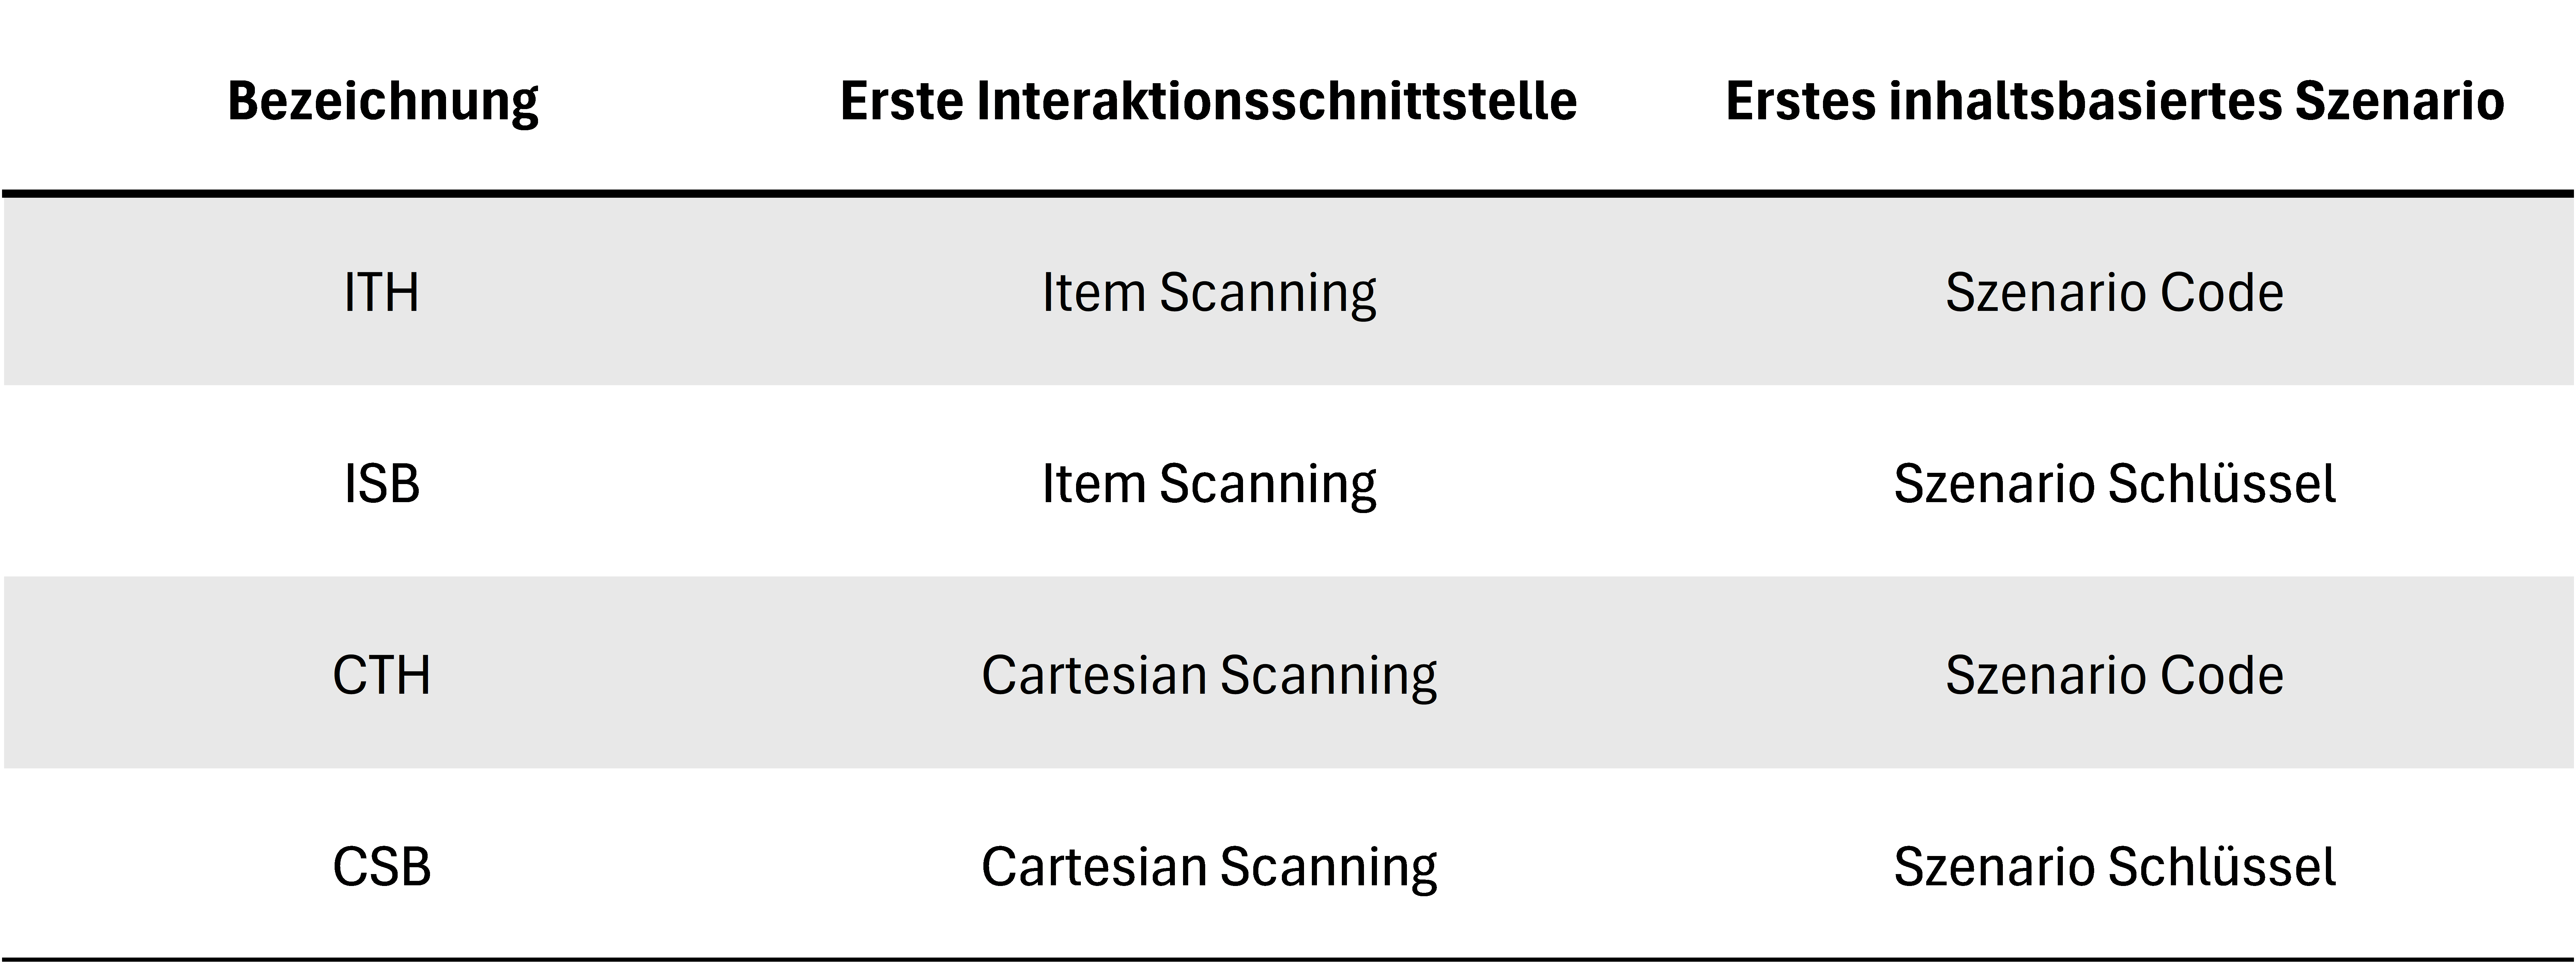
\includegraphics[scale=0.9]{images/Tabelle-Evaluationsgruppen.png}
    \caption{Testgruppen der Evaluation}
    \label{tab:Testgruppen}
\end{table}

\section{Ergebnisse}

\subsection{Usability (SUS) und User Experience (UEQ)}

Die Ergebnisse der SUS zeigen deutliche Unterschiede zwischen den beiden Schnittstellen. Der Mittelwert des SUS-Scores für das Item Scanning beträgt 73,44 (SD = 16,28) bei einem Median von 73,75. Für das Cartesian Scanning liegt der Mittelwert hingegen bei 85,63 (SD = 11,96) mit einem Median von 90. Die Ergebnisse werden in der \autoref{fig:resultsSUS} dargestellt. 

\begin{figure}[tbh]
    \centering
    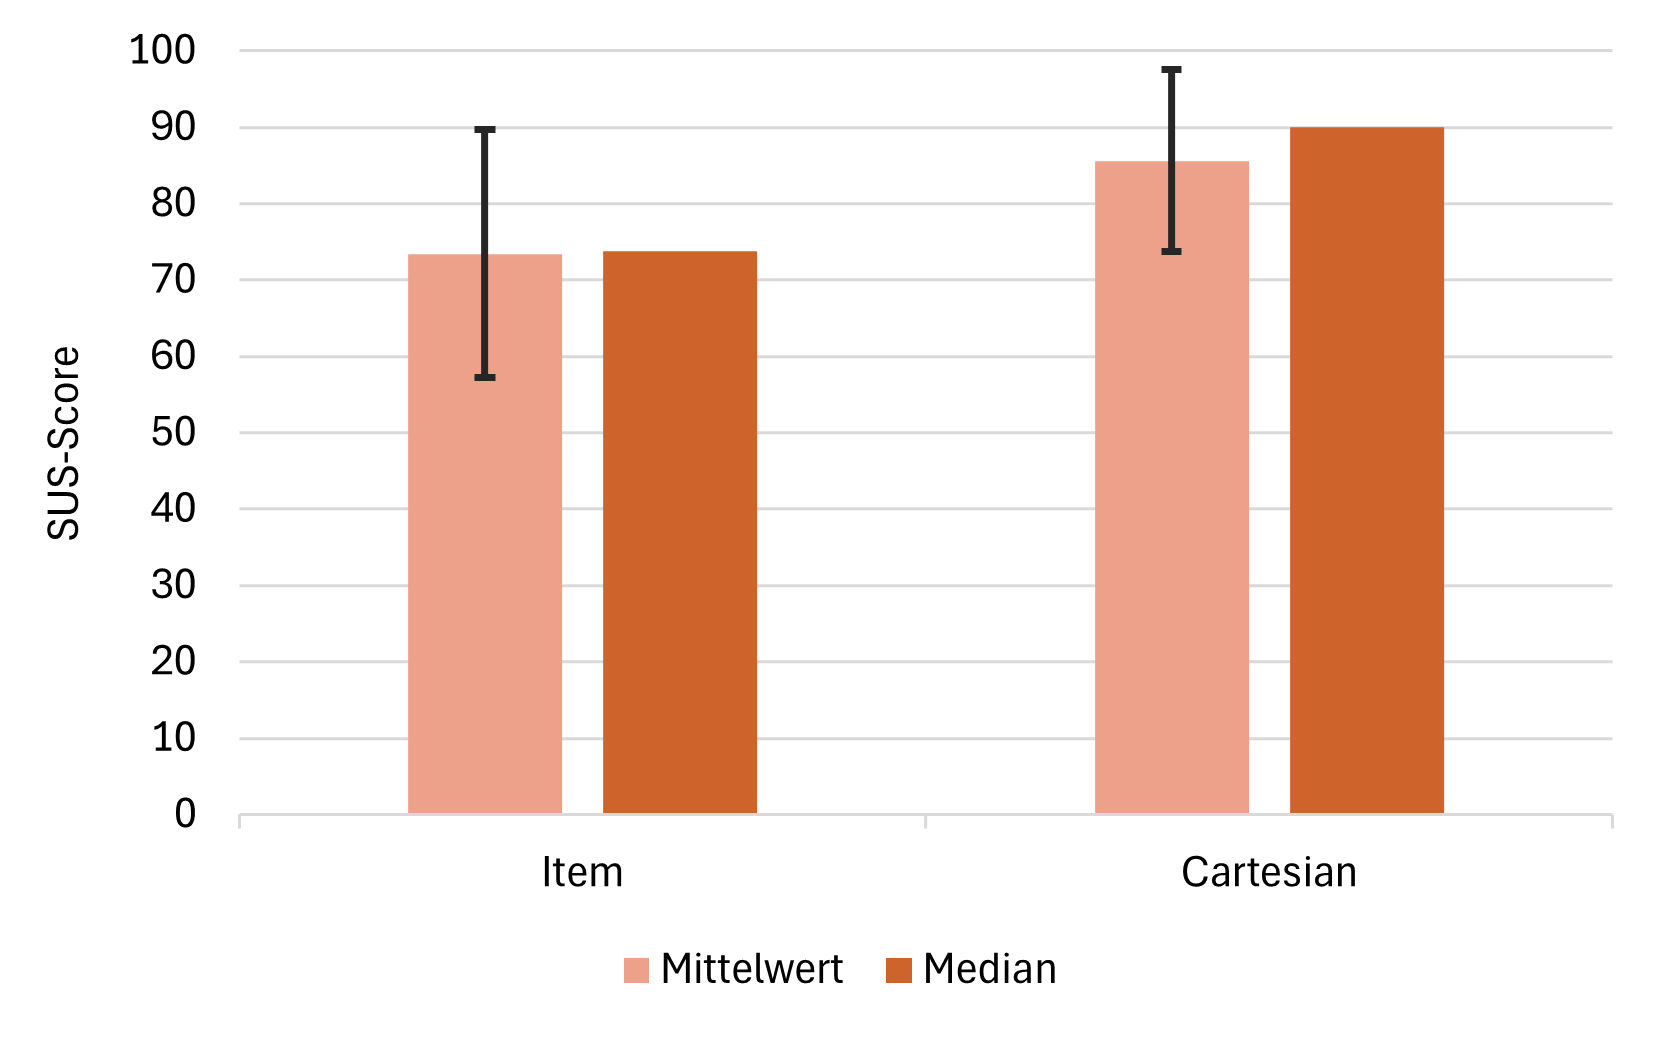
\includegraphics[scale=0.75]{images/Results/SUS-Scores.png}
    \caption{Mittelwerte und Median der SUS-Scores beider Interaktionsschnittstellen}
    \label{fig:resultsSUS}
\end{figure}

Die detaillierte Verteilung der Scores ist in \autoref{fig:histoSUS} dargestellt. Für das Item Scanning variieren die SUS-Scores zwischen 47,5 und 97,5. Der größte Anteil (drei Personen) liegt im Bereich 52,5-57,5. Insgesamt bewerteten sieben von 16 Teilnehmenden (43,75\%) die Schnittstelle mit einem Score von 80 oder höher. Für das Cartesian Scanning liegen die SUS-Scores zwischen 57,5 und 97,5. Der größte Anteil der Teilnehmenden (sechs Personen) bewertete die Schnittstelle mit einem Score im Bereich 92,5-97,5. Insgesamt haben 11 von 16 Teilnehmenden (68,75\%) die Schnittstelle mit einem SUS-Score von mindestens 80 bewertet. 

\begin{figure}
    \centering
    \begin{subfigure} {.5\textwidth}
        \centering
        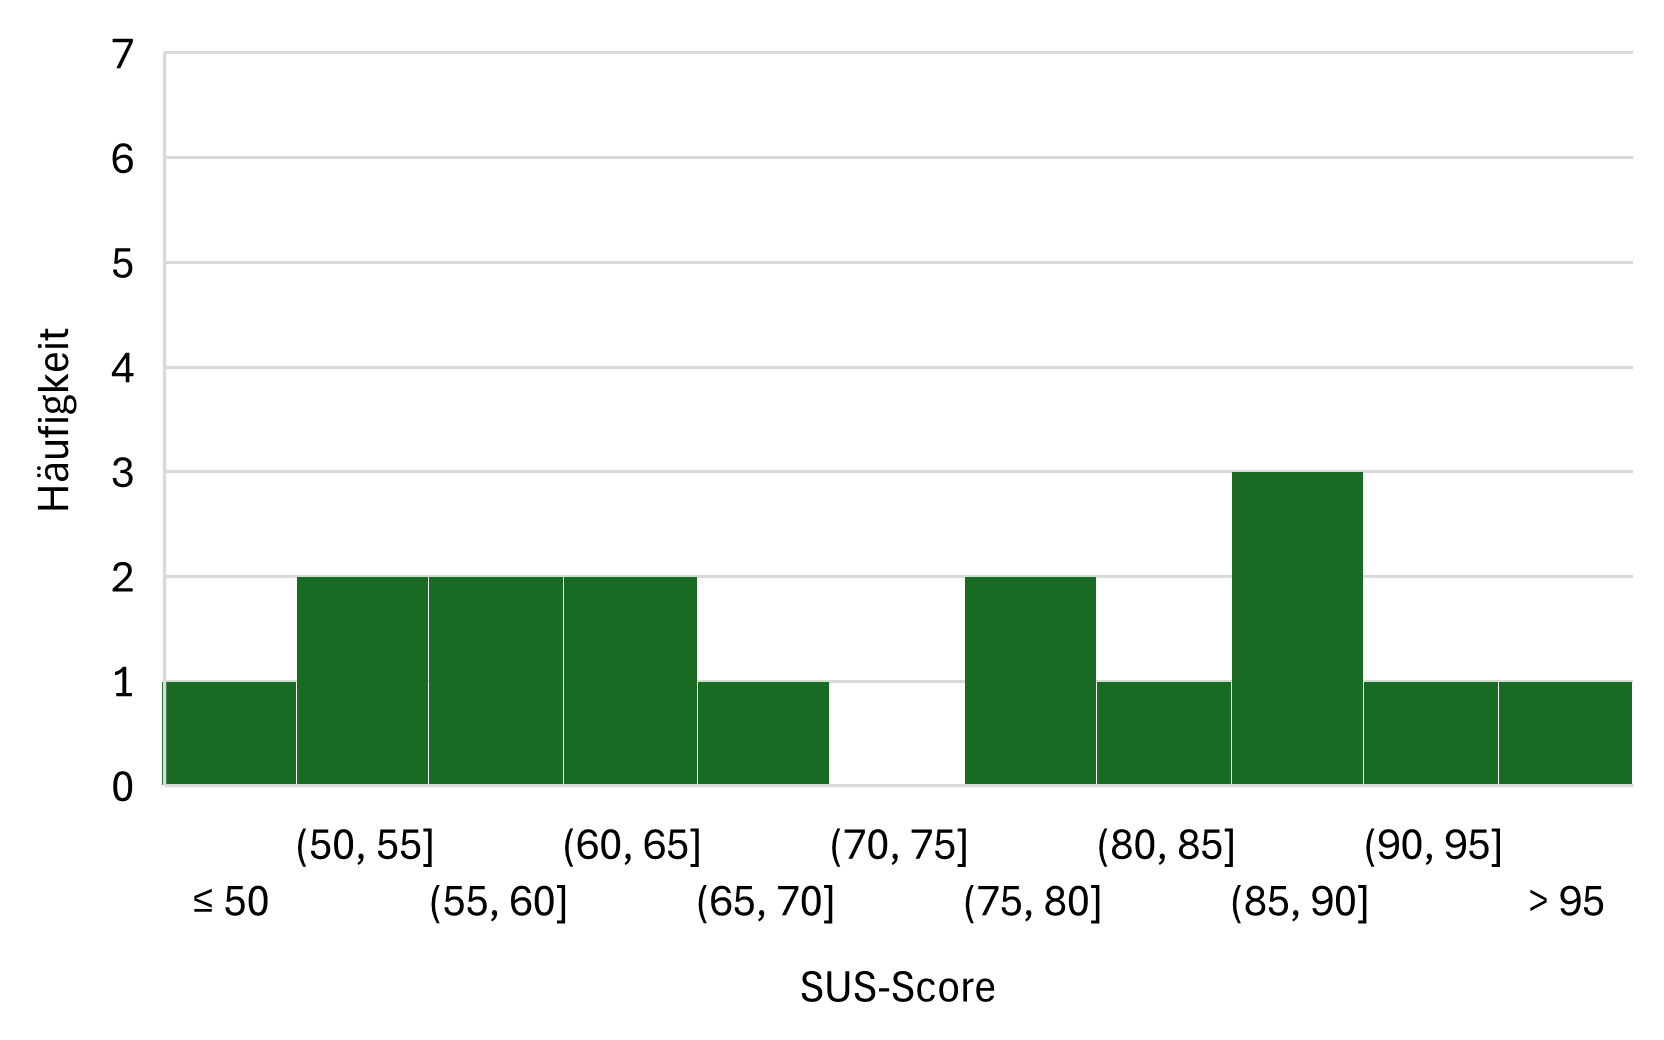
\includegraphics[width=.95\linewidth]{images/Results/Histogramm-SUS-Item.png}
        \caption{Item Scanning}
        \label{fig:histoSUSItem}
       \end{subfigure}%
       \begin{subfigure}{.5\textwidth}
        \centering
       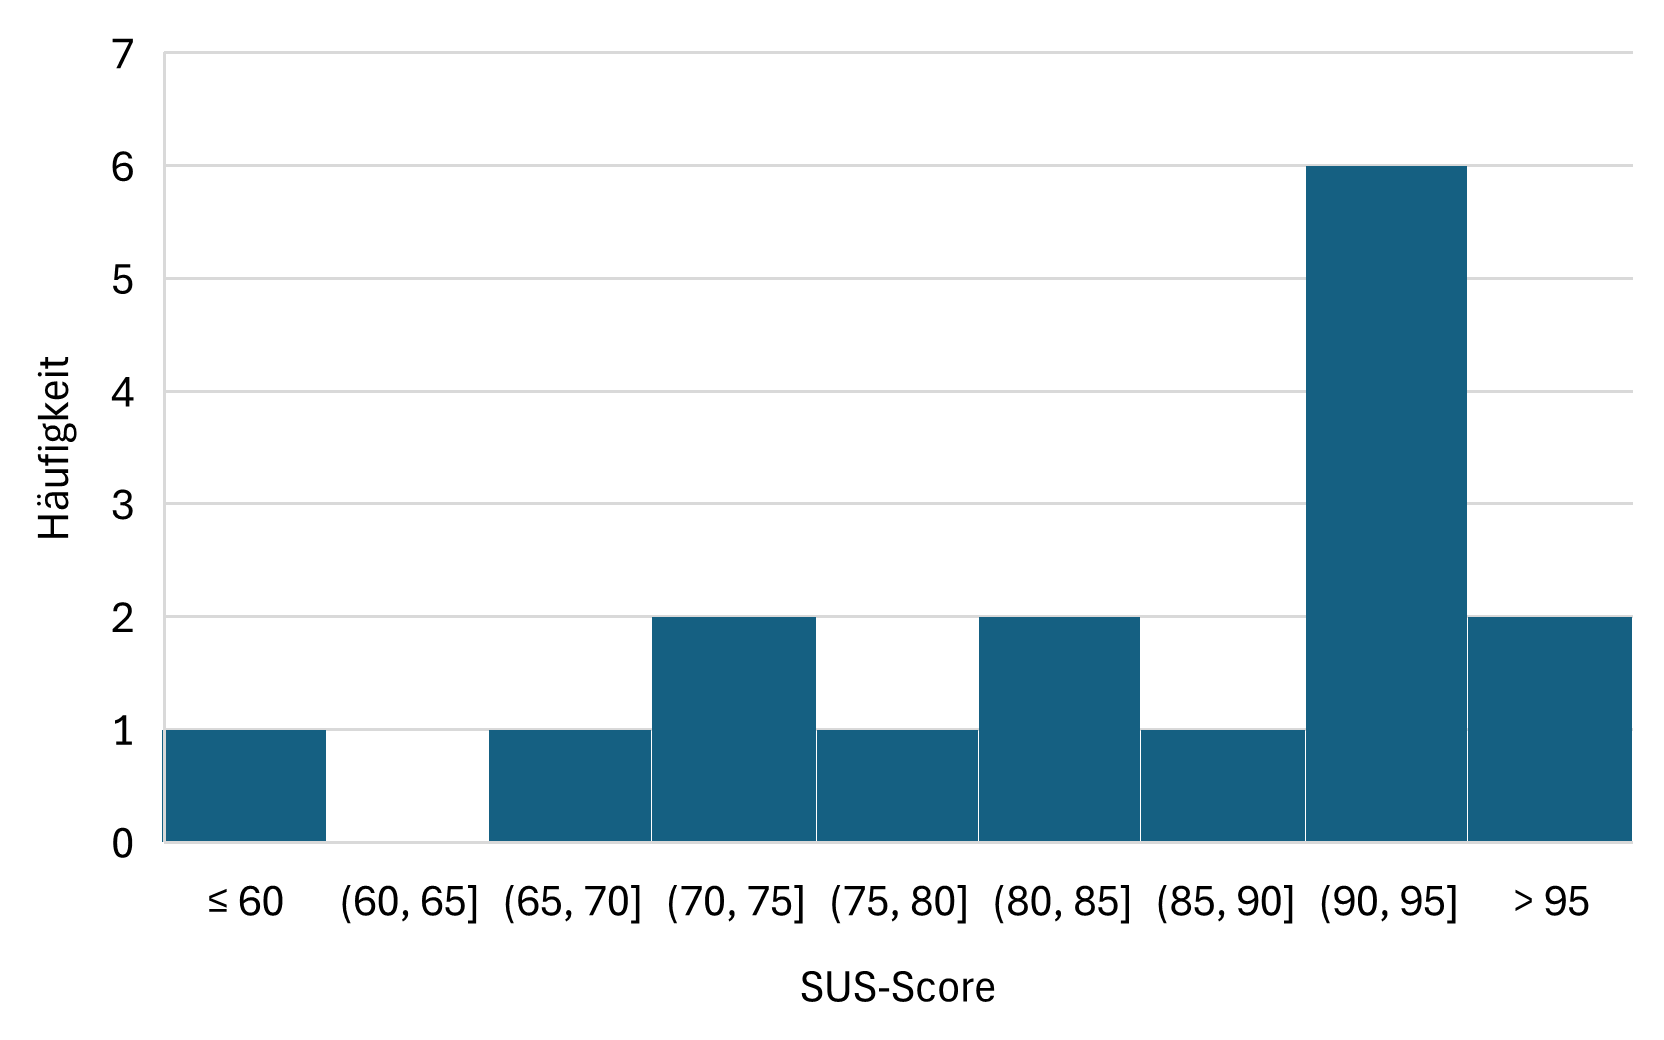
\includegraphics[width=.98\linewidth]{images/Results/Histogramm-SUS-Cartesian.png}
        \caption{Cartesian Scanning}
        \label{fig:histoSUSCartesian}
       \end{subfigure}
       \caption{Verteilung der SUS Scores beider Interaktionsschnittstellen}
       \label{fig:histoSUS}
\end{figure}


Die Ergebnisse des UEQ wurden mit Hilfe des Auswertungstools der Autoren analysiert. Für jeden der sechs Faktoren wurden Mittelwerte und Varianzen berechnet. Die \autoref{tab:ueqScalesItem} zeigt die berechneten Mittelwerte und Varianzen für das Item Scanning. In \autoref{fig:ueqScoreItem} werden diese Ergebnisse zusätzlich visualisiert.

\begin{table}[tbh]
    \centering
    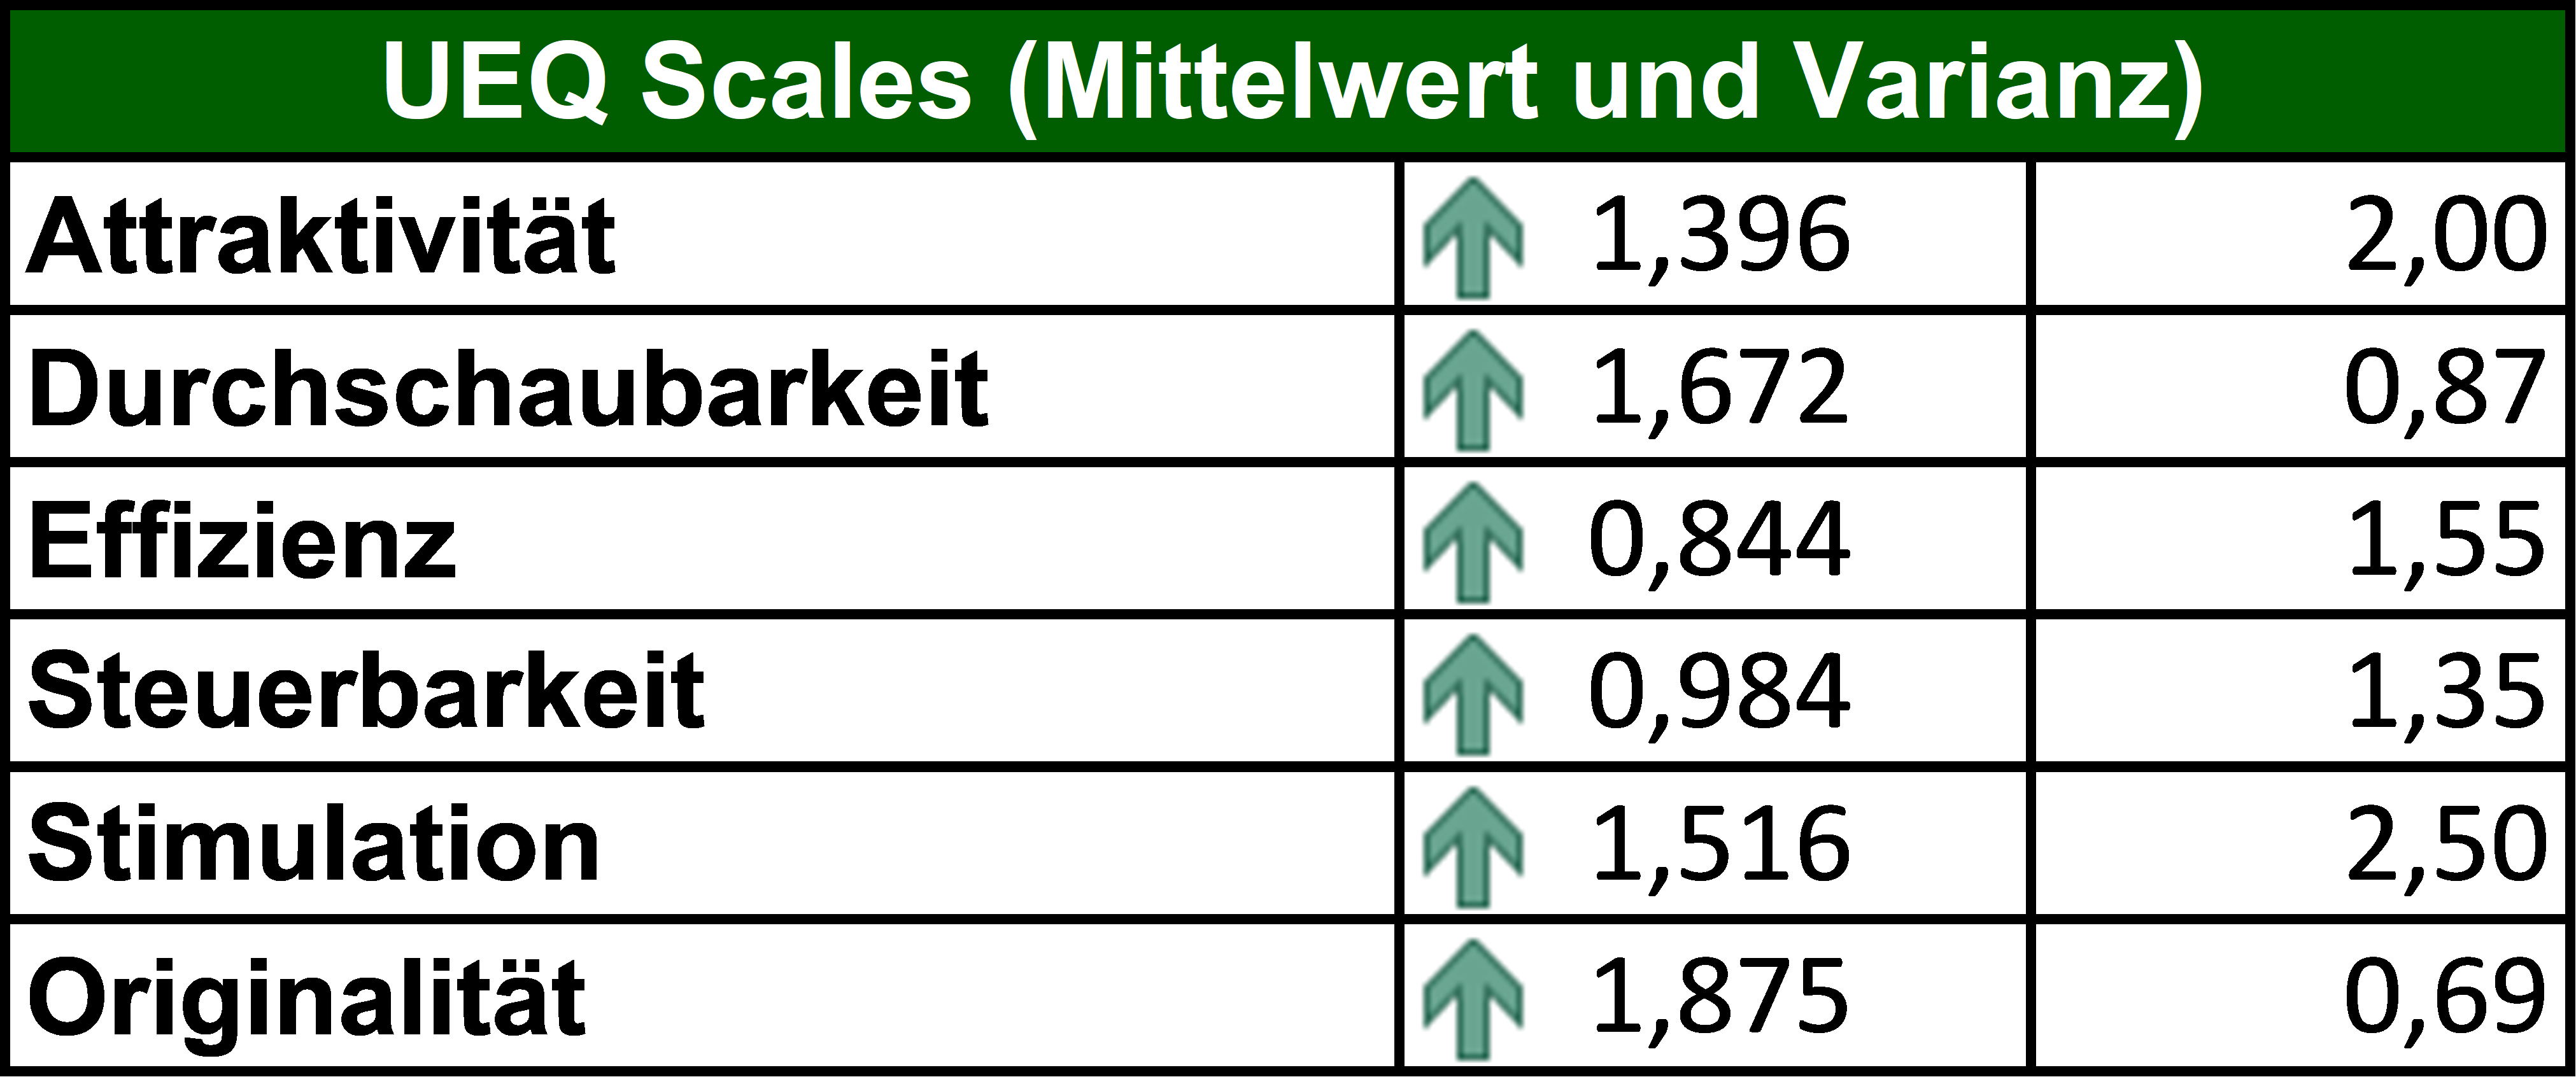
\includegraphics{images/Results/UEQ-Table-Means-Item.png}
    \caption{UEQ-Ergebnisse des Item Scanning}
    \label{tab:ueqScalesItem}
\end{table}

\begin{figure}[tbh]
    \centering
    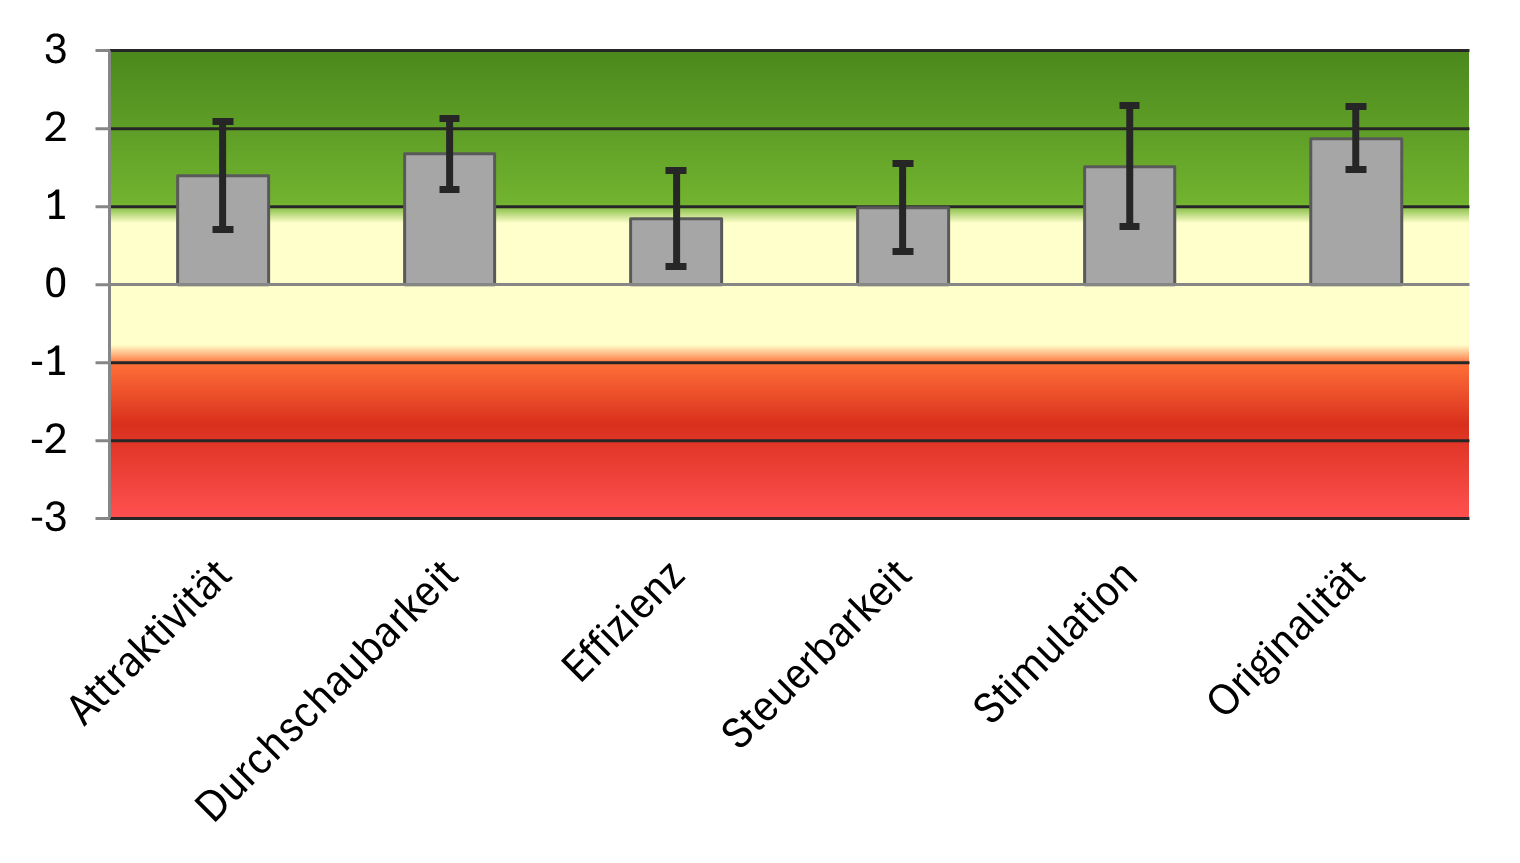
\includegraphics{images/Results/UEQ-Item.png}
    \caption{Visualisierung der UEQ-Ergebnisse des Item Scanning}
    \label{fig:ueqScoreItem}
\end{figure}

Für das Item Scanning liegen die Mittelwerte der Bewertungen im positiven Bereich. Den höchsten Wert weist der Faktor Originalität mit einem Mittelwert (MW) von 1,875 bei einer Varianz von 0,69 auf, gefolgt von Durchschaubarkeit (MW = 1,672, Varianz = 0,87) und Stimulation (MW = 1,516, Varianz = 2,50). Am niedrigsten wurden die Faktoren Steuerbarkeit und Effizienz bewertet. Hier liegen die Mittelwerte bei 0,984 und 0,844 mit Varianzen von 1,35 und 1,55. 

Die Ergebnisse für das Cartesian Scanning sind in \autoref{tab:ueqScalesCartesian} dargestellt und in \autoref{fig:ueqScoreCartesian} visualisiert. 

Das Cartesian Scanning wurde insgesamt besser bewertet als das Item Scanning. Der Faktor Durchschaubarkeit wurde mit einem Mittelwert von 2,234 und einer Varianz von 0,53 am höchsten bewertet. Die Faktoren Attraktivität, Stimulation und Originalität wurden mit Mittelwerten von 1,833, 1,734 und 1,750 ähnlich hoch bewertet. Den niedrigsten Mittelwert und gleichzeitig die höchste Varianz weist der Faktor Effizienz auf. Hier liegt der Mittelwert bei 1,063 bei einer Varianz von 1,33. 

Im Anhang in \autoref{Anhang:Ergebnisse} sind ergänzend die detaillierten Verteilungen der Bewertungen der einzelnen Items des UEQ für beide Schnittenstellen aufgeführt. 

\begin{table}[tbh]
    \centering
    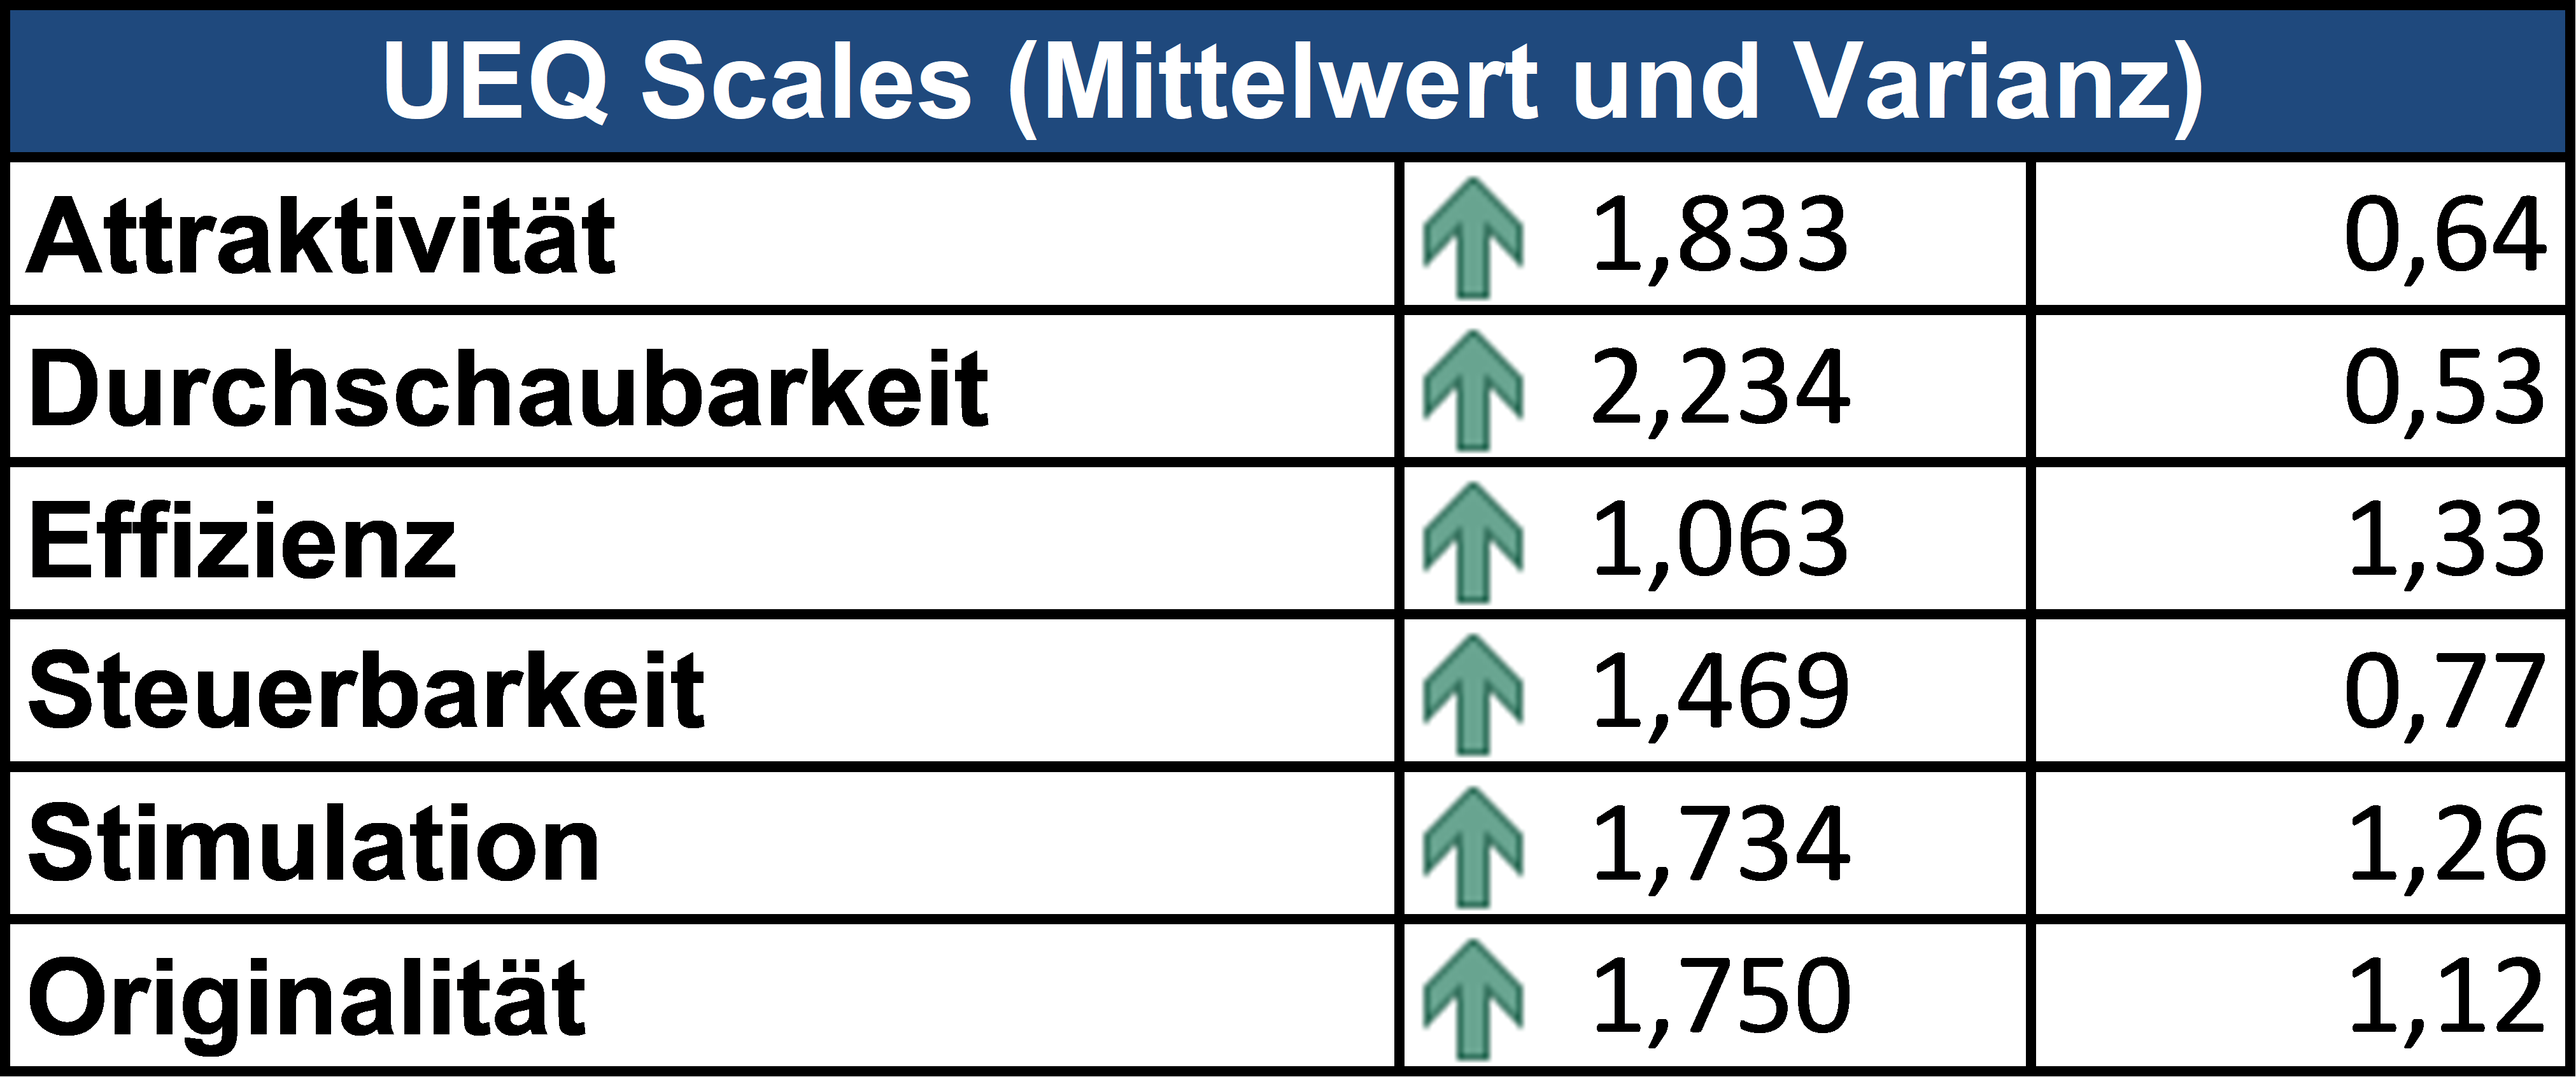
\includegraphics{images/Results/UEQ-Table-Means-Cartesian.png}
    \caption{UEQ-Ergebnisse des Cartesian Scanning}
    \label{tab:ueqScalesCartesian}
\end{table}

\begin{figure}[tbh]
    \centering
    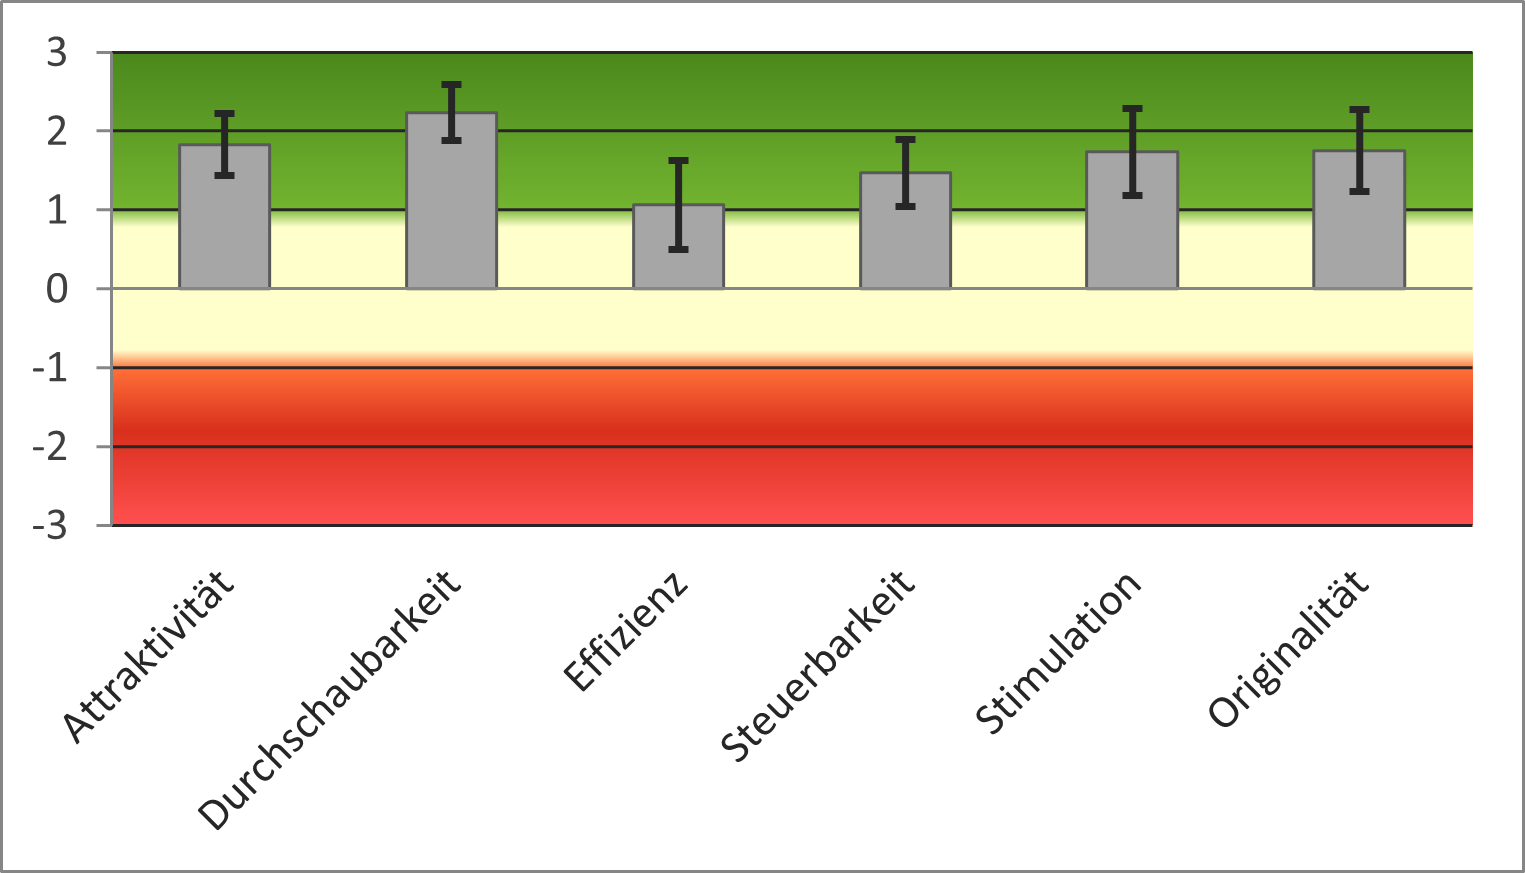
\includegraphics{images/Results/UEQ-Cartesian.png}
    \caption{Ergebnisse UEQ Cartesian Scanning}
    \label{fig:ueqScoreCartesian}
\end{figure}


\subsection{Motion Sickness (SSQ)} 

Die Ergebnisse des SSQ werden in \autoref{tab:tableSymptomsSSQ} dargestellt. Die Tabelle zeigt die im Fragebogen erfassten Symptome sowie die jeweilige Symptomkategorie (N: Nausea, O: Oculomotor, D: Disorientation). Für beide Schnittstellen wird für jedes Symptom die Häufigkeit angegeben, mit der es auftrat. Dies entspricht der Anzahl der Personen, die einen Wert >0 angaben. Zusätzlich wird in einer weiteren Spalte dargestellt, wie viele dieser Personen in der Auswertung jeweils einen Wert >1 angegeben haben und somit eine moderate bis starke Ausprägung des Symptoms empfunden haben. 
Es zeigt sich, dass beim Item Scanning die Symptome angestrengte Augen (11 Personen, davon vier mit moderater Ausprägung) sowie Ermüdung, Kopfdruck und verschwommenes Sehen (sechs Personen, keine moderaten Ausprägungen) am häufigsten auftraten. Vereinzelt wurde von allgemeinem Unwohlsein, Konzentrationsschwierigkeiten, Schwitzen, erhöhtem Speichelfluss, Schwindel und Übelkeit berichtet, wobei diese Symptome jeweils nur eine oder zwei Personen betrafen und nur in leichter Ausprägung auftraten. Symptome wie Aufstoßen oder Gleichgewichtsstörungen wurden nicht genannt.
Beim Cartesian Scanning ergab sich eine ähnliche Verteilung. Am häufigsten wurden angestrengte Augen (11 Personen, davon zwei mit moderater Ausprägung) und Ermüdung (acht Personen, keine moderaten Ausprägungen) berichtet. Im Vergleich zum Item Scanning traten verschwommenes Sehen und Kopfdruck etwas seltener auf (drei bzw. vier Personen). Weitere Symptome wie Konzentrationsschwierigkeiten oder Schwitzen traten ebenfalls nur vereinzelt auf, während allgemeines Unwohlsein, Übelkeit und Gleichgewichtsstörungen nicht aufgetreten sind.

\begin{table}[tbh]
    \centering
    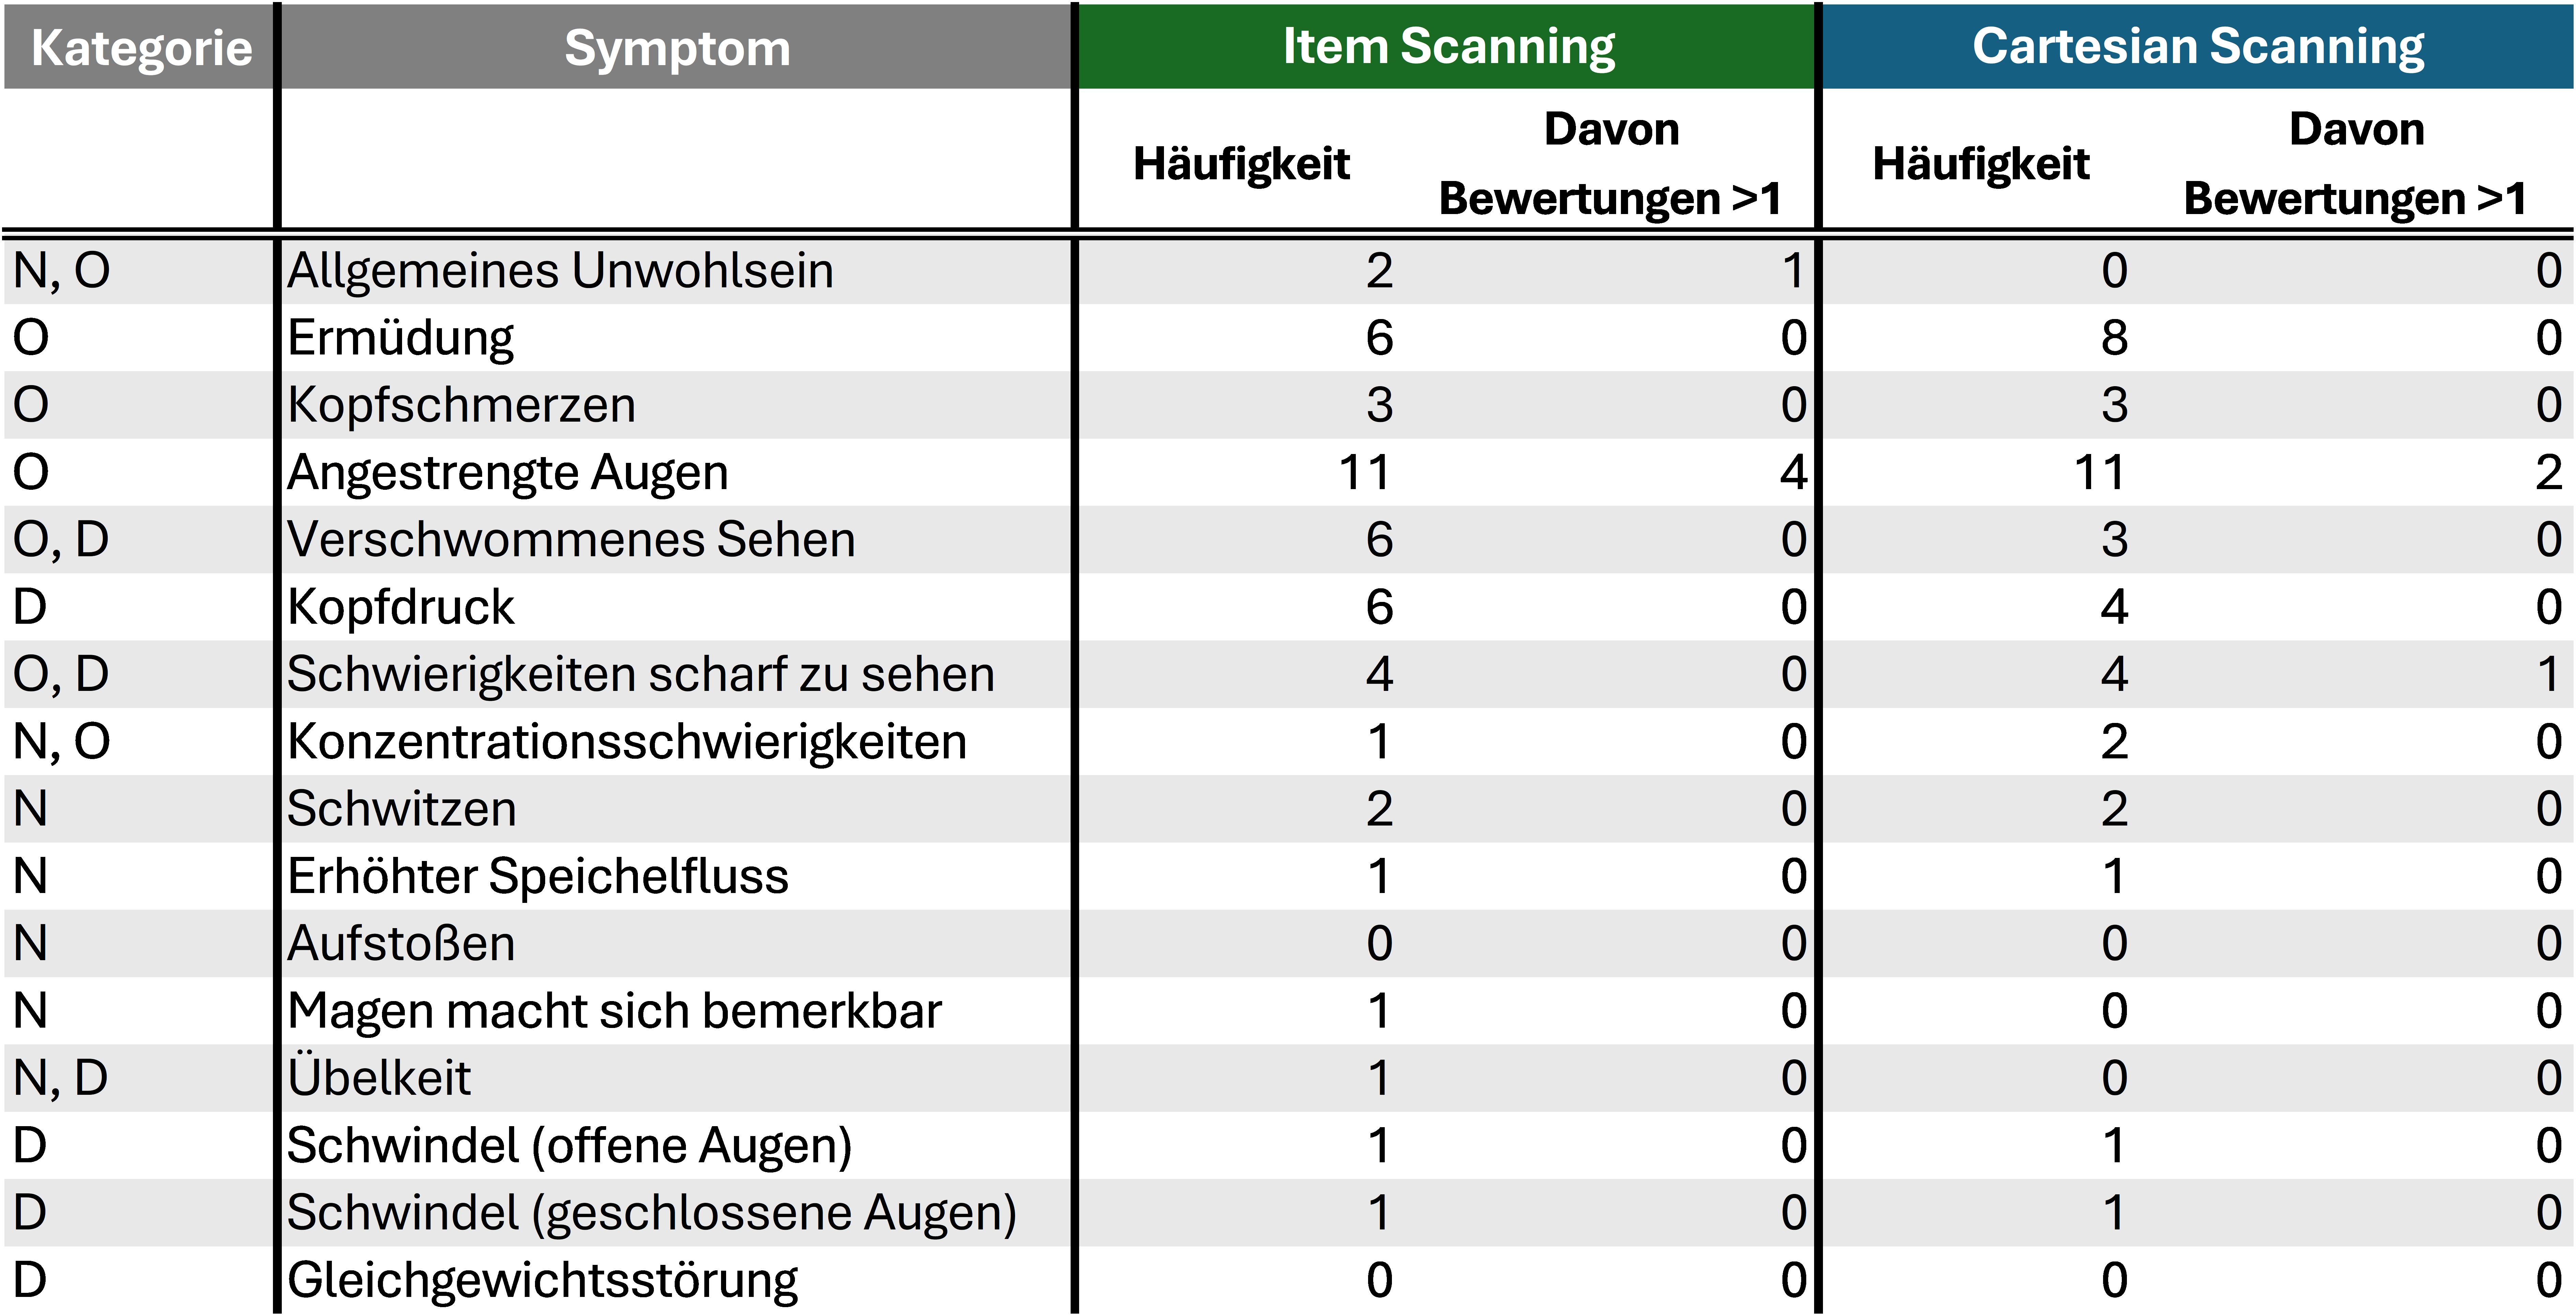
\includegraphics[width=0.95\textwidth]{images/Results/SSQ-Table-2.png}
    \caption{Häufigkeit der SSQ-Symptome beider Interaktionsschnittstellen}
    \label{tab:tableSymptomsSSQ}
\end{table}

Die weitere Auswertung des SSQ erfolgte nach der Beschreibung der Autoren \citep{kennedy_simulator_1993}. Dazu wurden zunächst die gewichteten Scores der einzelnen Kategorien und anschließend der Gesamtscore bestimmt. Die Ergebnisse sind in \autoref{tab:tableErgebnisseSSQ} dargestellt. Die Verteilung der Gesamtscores ist darüber hinaus in \autoref{fig:histoSSQScore} visualisiert. 

\begin{table}[tbh]
    \centering
    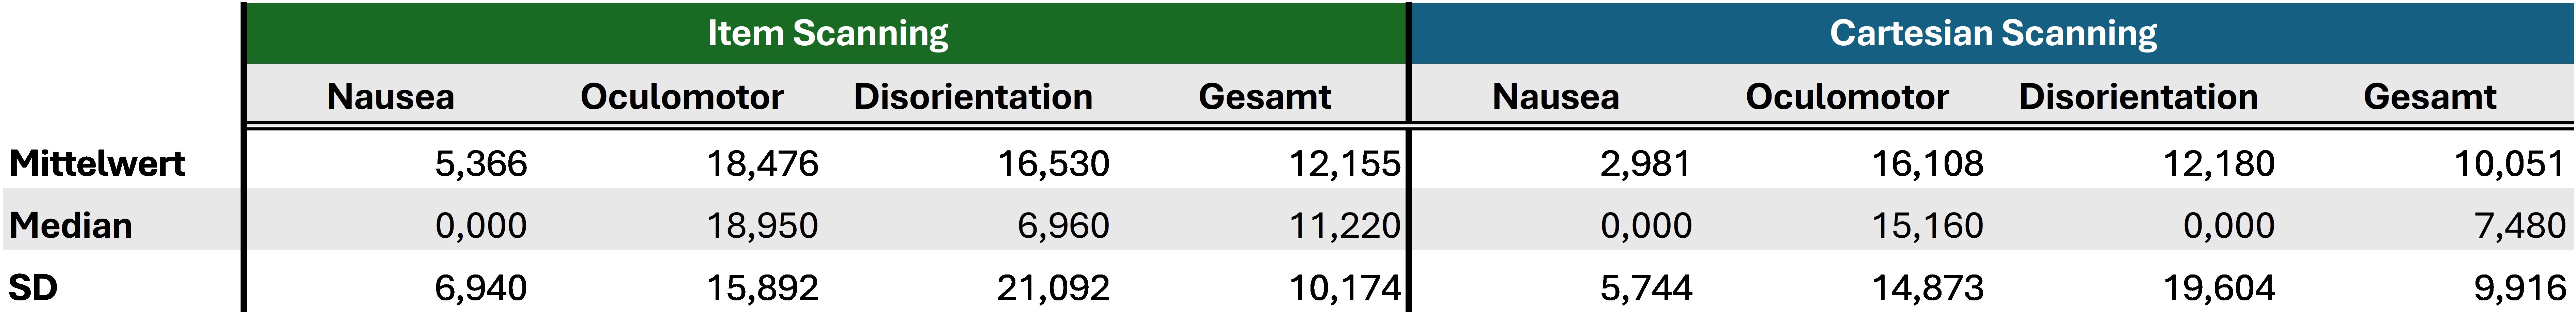
\includegraphics[width=0.95\textwidth]{images/Results/Tabelle-Ergebnisse-SSQ.png}
    \caption{Mittelwerte der SSQ-Ergebnisse nach Interaktionsschnittstelle und Kategorie}
    \label{tab:tableErgebnisseSSQ}
\end{table}

\begin{figure}
    \centering
    \begin{subfigure}{.5\textwidth}
        \centering
        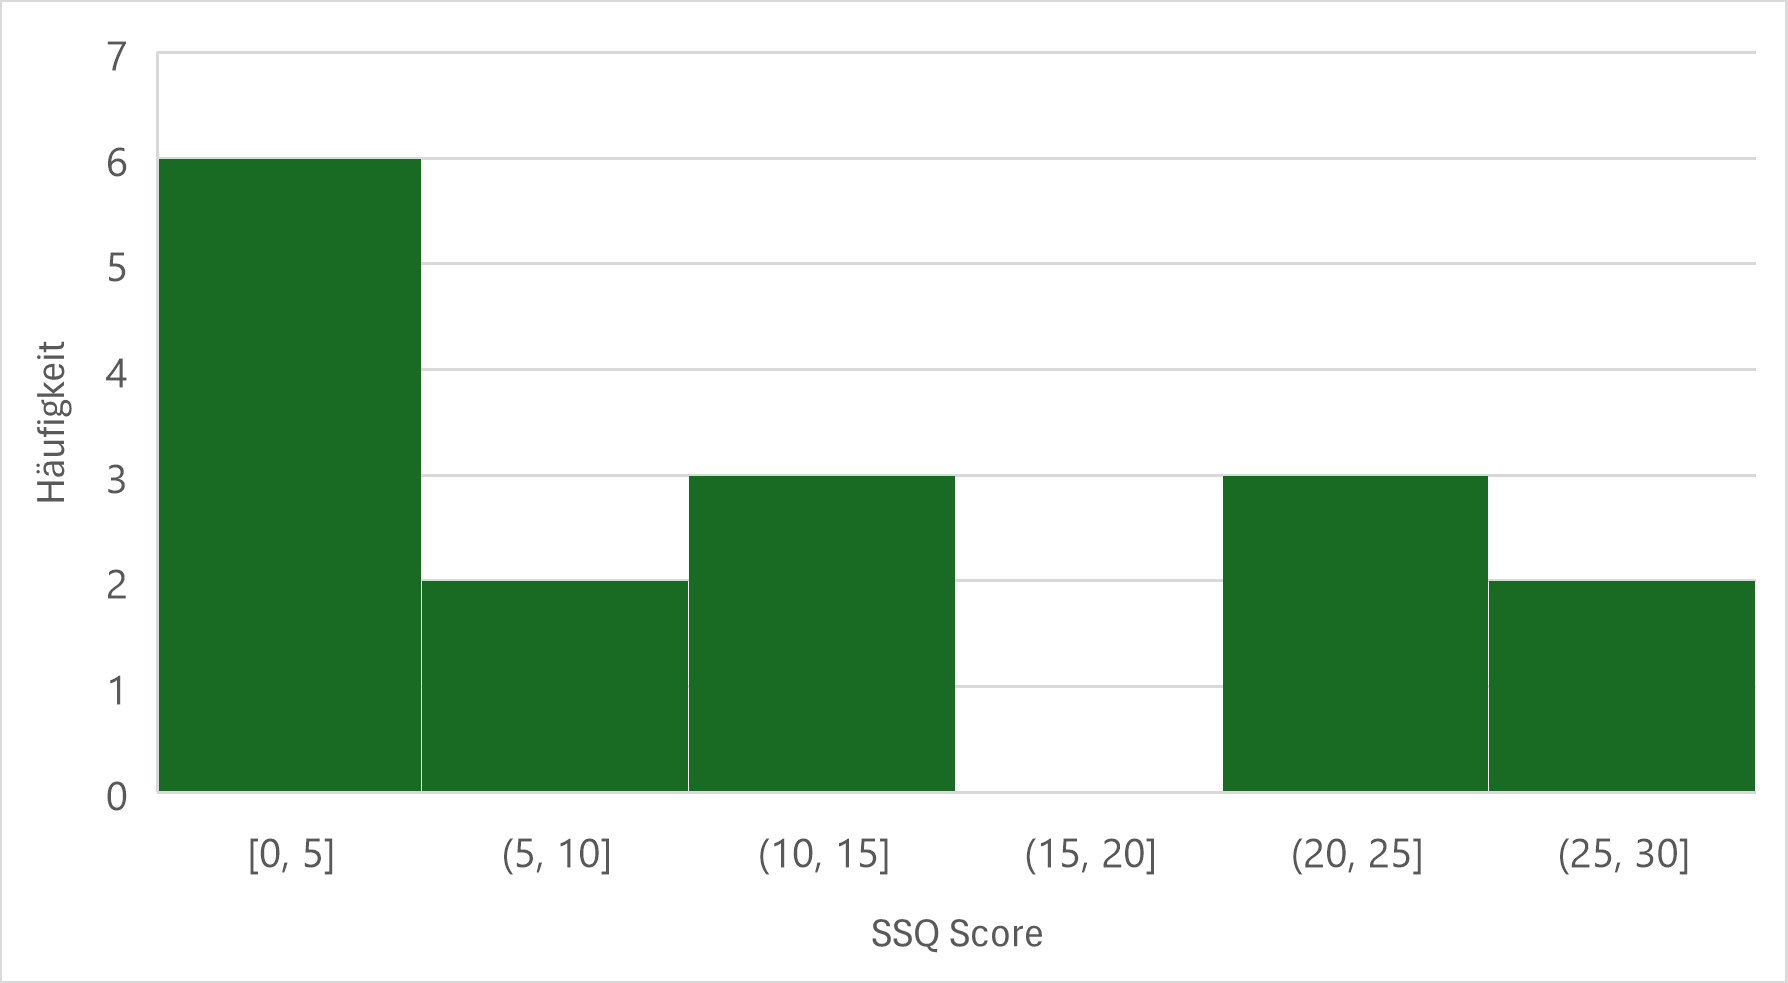
\includegraphics[width=0.99\textwidth]{images/Results/Histogramm-SSQScores-Item.png}
        \caption{Item Scanning}
        \label{fig:histoSSQItem}   
    \end{subfigure}%
    \begin{subfigure}{.5\textwidth}
        \centering
        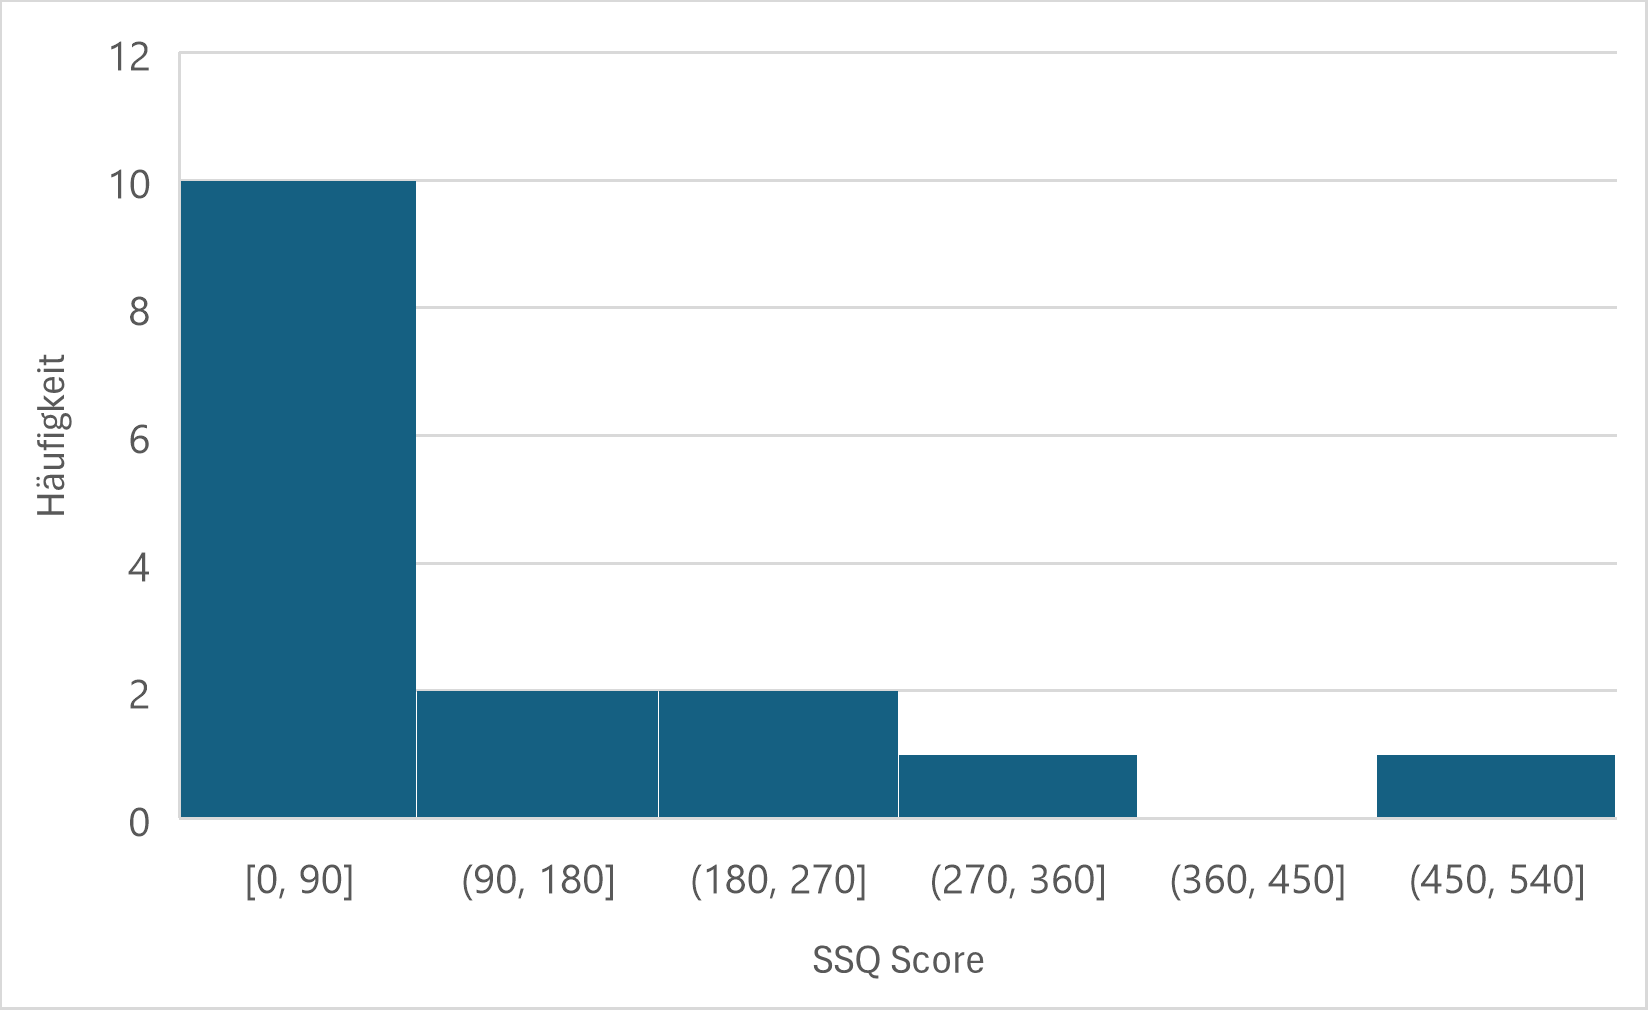
\includegraphics[width=0.99\textwidth]{images/Results/Histogramm-SSQScores-Cartesian.png}
         \caption{Cartesian Scanning}
         \label{fig:histoSSQCartesian}
    \end{subfigure}
    \caption{Verteilung der SSQ-Scores beider Interaktionsschnittstellen}
    \label{fig:histoSSQScore}
\end{figure}

Die Histogramme zeigen, dass die meisten Teilnehmenden bei beiden Schnittstellen einen SSQ-Wert zwischen 0 und 5 aufwiesen (jeweils sechs Personen). Beim Cartesian Scanning liegt der höchste Score bei 37,40 und damit deutlich höher als beim Item Scanning (29,92). Allerdings erreichten beim Item Scanning insgesamt mehr Personen einen Score größer 10 (acht Personen gegenüber sechs Personen). Der Mittelwert des Gesamtscores liegt beim Item Scanning bei 12,155 (SD = 10,174) und beim Cartesain Scanning bei 10,051 (SD = 9,916) (vgl. \autoref{tab:tableErgebnisseSSQ}).

Um genauere Aussagen darüber treffen zu können, in welchen Kategorien die meisten Symptome auftraten, werden die Ergebnisse der Scores der Kategorien folgend genauer betrachtet.

\begin{figure}
    \centering
    \begin{subfigure}{.5\textwidth}
        \centering
        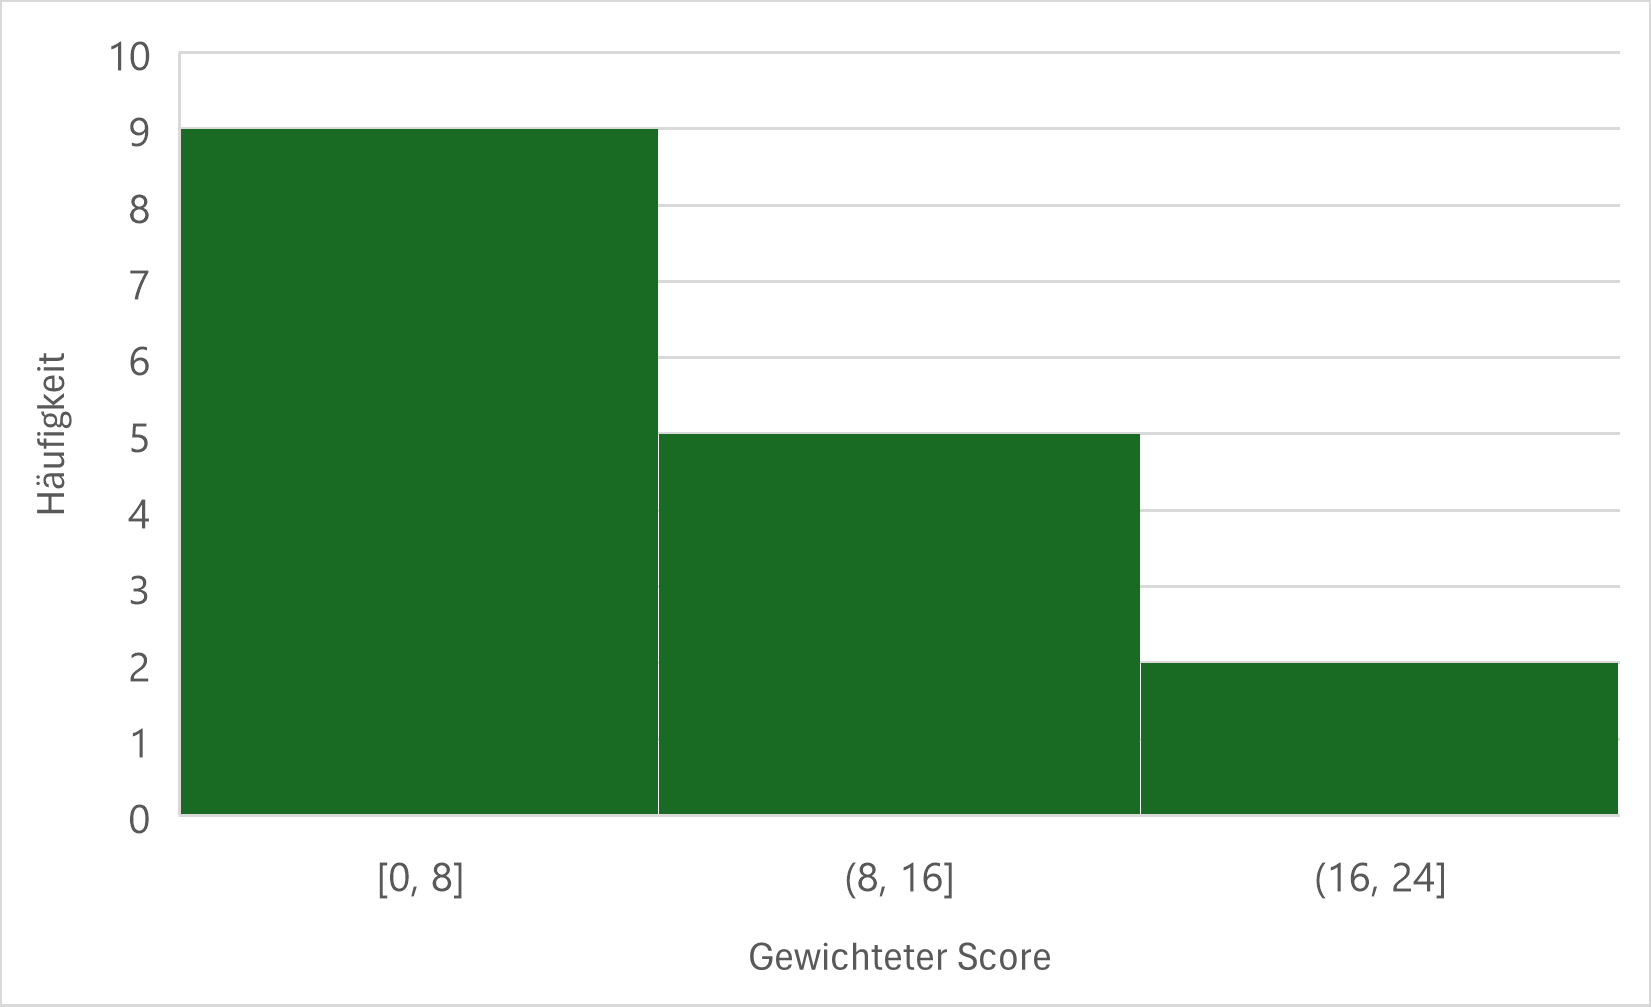
\includegraphics[width=0.99\textwidth]{images/Results/Histogramm-Nausea-Scale-Item.png}
        \caption{Item Scanning}
        \label{fig:histoNauseaItem}   
    \end{subfigure}%
    \begin{subfigure}{.5\textwidth}
        \centering
        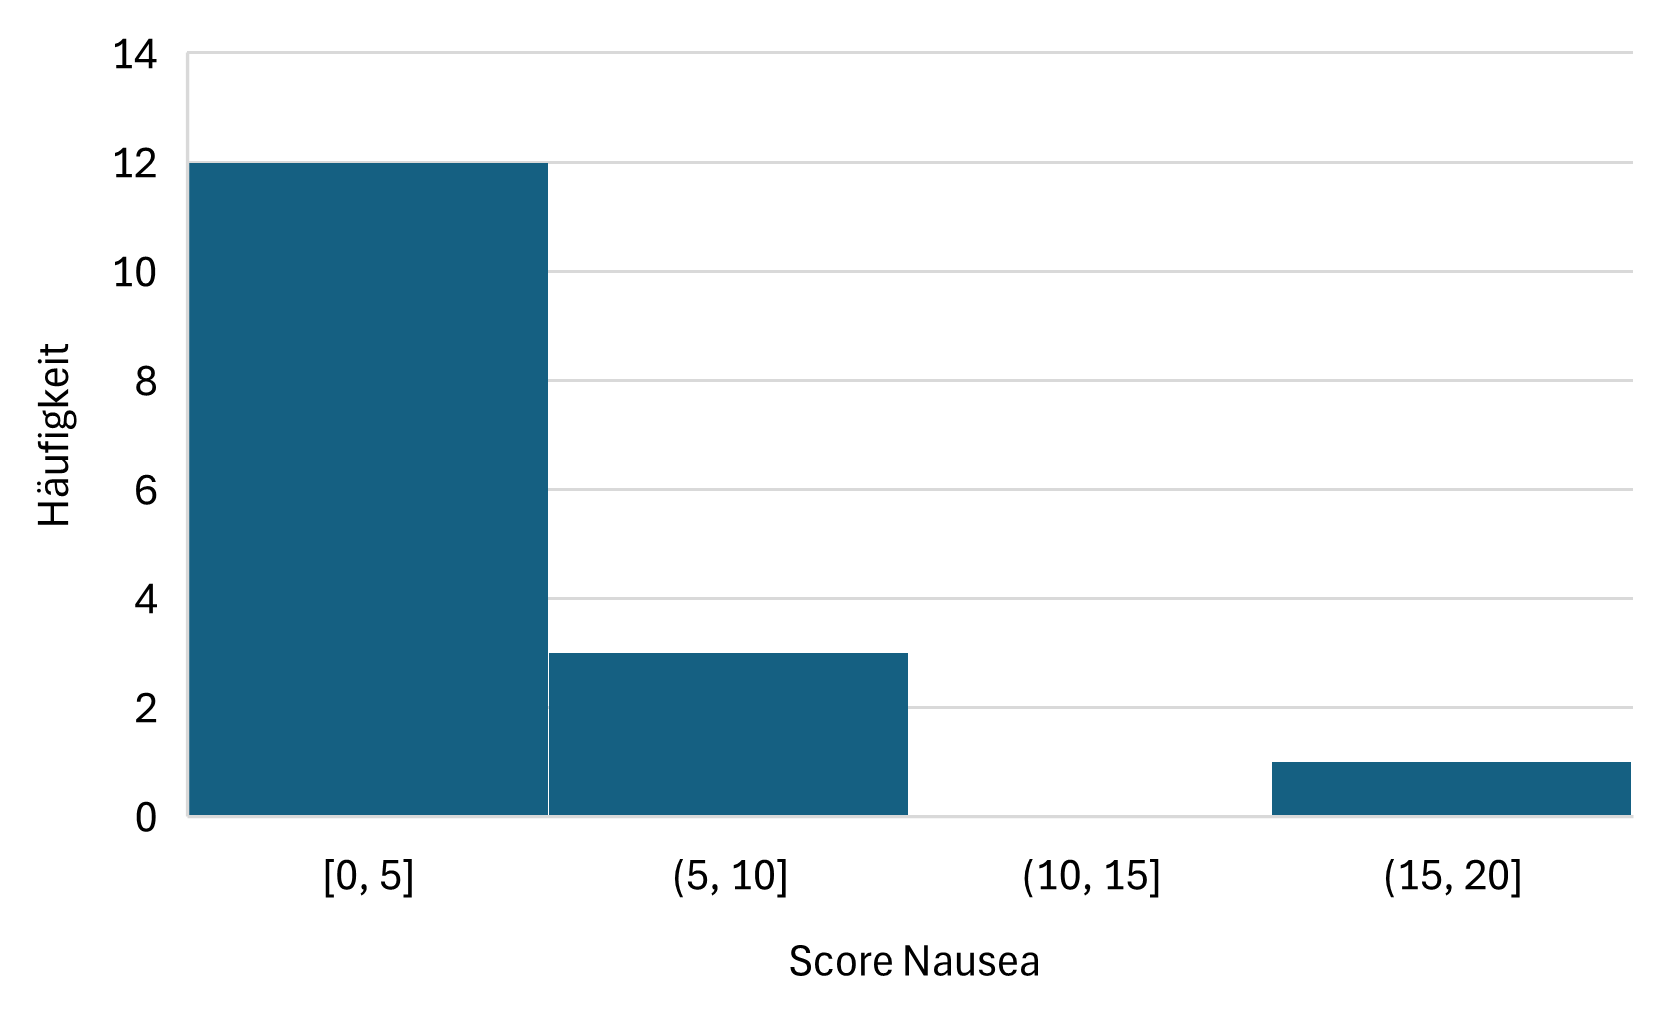
\includegraphics[width=0.99\textwidth]{images/Results/Histogramm-Nausea-Scale-Cartesian.png}
         \caption{Cartesian Scanning}
         \label{fig:histoNauseaCartesian}
    \end{subfigure}
    \caption{Verteilung der Scores der SSQ Nausea Scale beider Interaktionsschnittstellen}
    \label{fig:histoNausea}
\end{figure}

In der Kategorie Nausea (vgl. \autoref{fig:histoNausea}) berichteten beim Item Scanning neun Personen keine Symptome. Fünf Teilnehmende zeigten Scores zwischen 8 und 10, was dem Auftreten eines einzigen Symptoms in leichter Ausprägung entspricht. Zwei Personen erreichten Scores über 15, was dem Auftreten mehrerer Symptome oder mindestens einem Symptom in moderater bis starker Ausprägung entspricht. Der Mittelwert der Scores dieser Kategorie liegt bei 5,366 (SD = 6,940) (vgl. \autoref{tab:tableErgebnisseSSQ}). Beim Cartesian Scanning hingegen zeigten 12 Personen keine Symptome. Drei Personen erreichten einen Score zwischen 5 und 10 und eine Person einen Score über 15. Der Mittelwert für das Cartesian Scanning in dieser Kategorie liegt bei 2,981 (SD = 5,744) (vgl. \autoref{tab:tableErgebnisseSSQ}).

\begin{figure}
    \centering
    \begin{subfigure}{.5\textwidth}
        \centering
        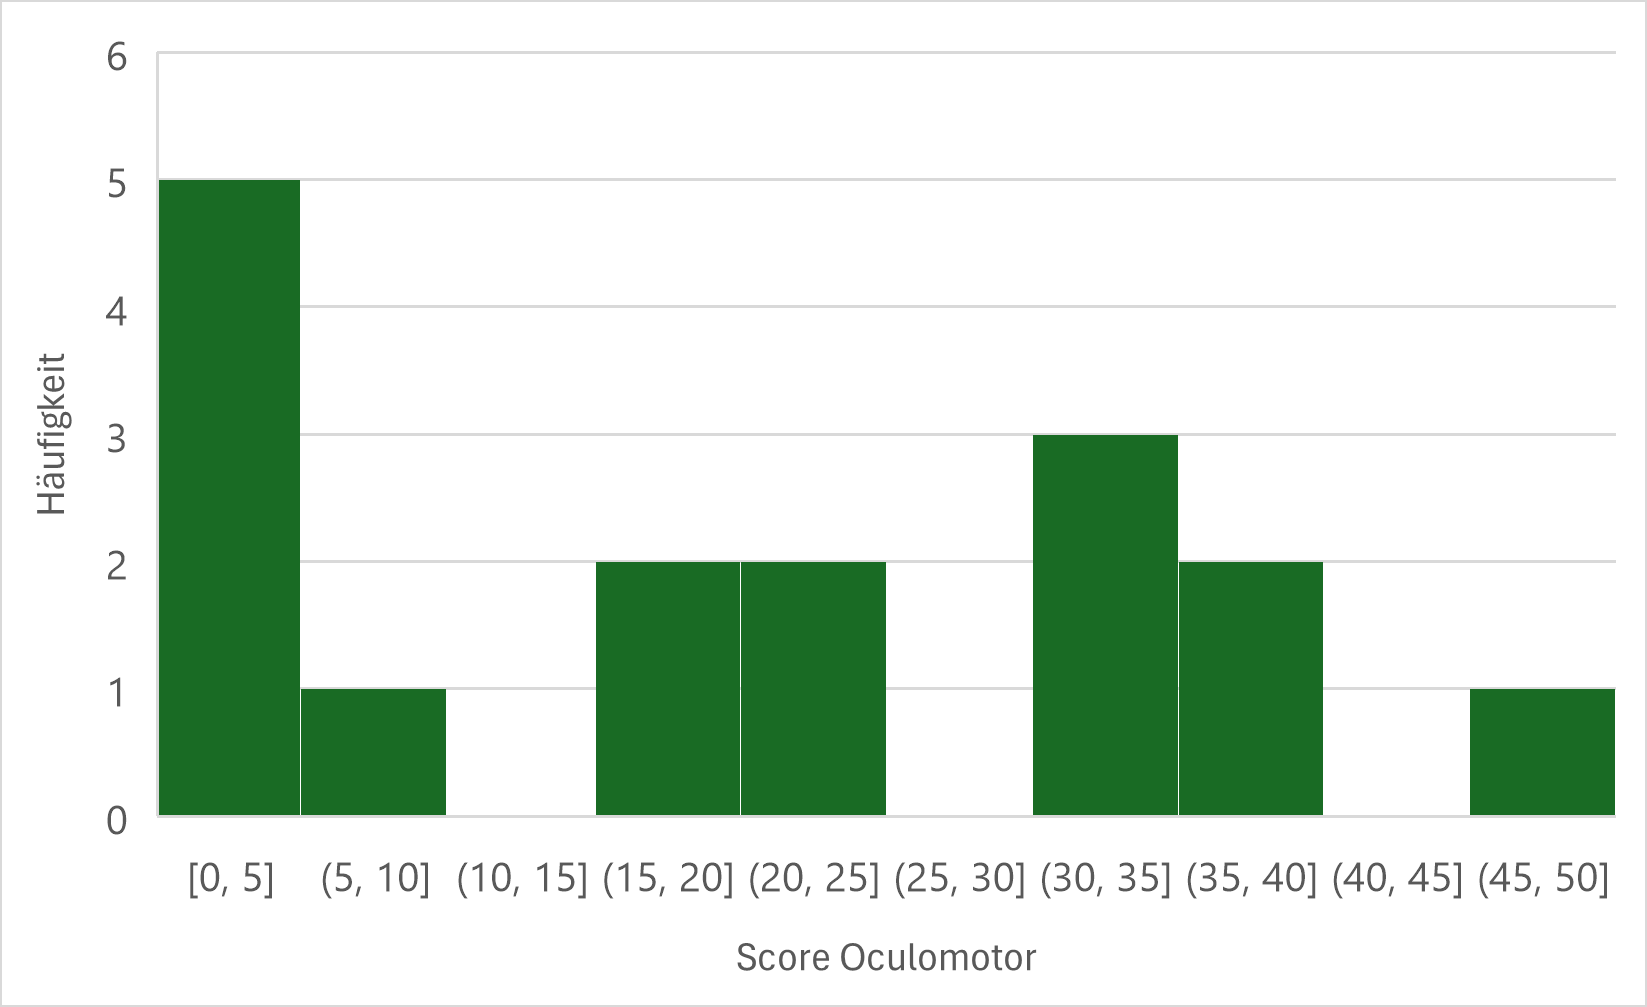
\includegraphics[width=0.99\textwidth]{images/Results/Histogramm-Oculomotor-Scale-Item.png}
        \caption{Item Scanning}
        \label{fig:histoOculomotorItem}   
    \end{subfigure}%
    \begin{subfigure}{.5\textwidth}
        \centering
        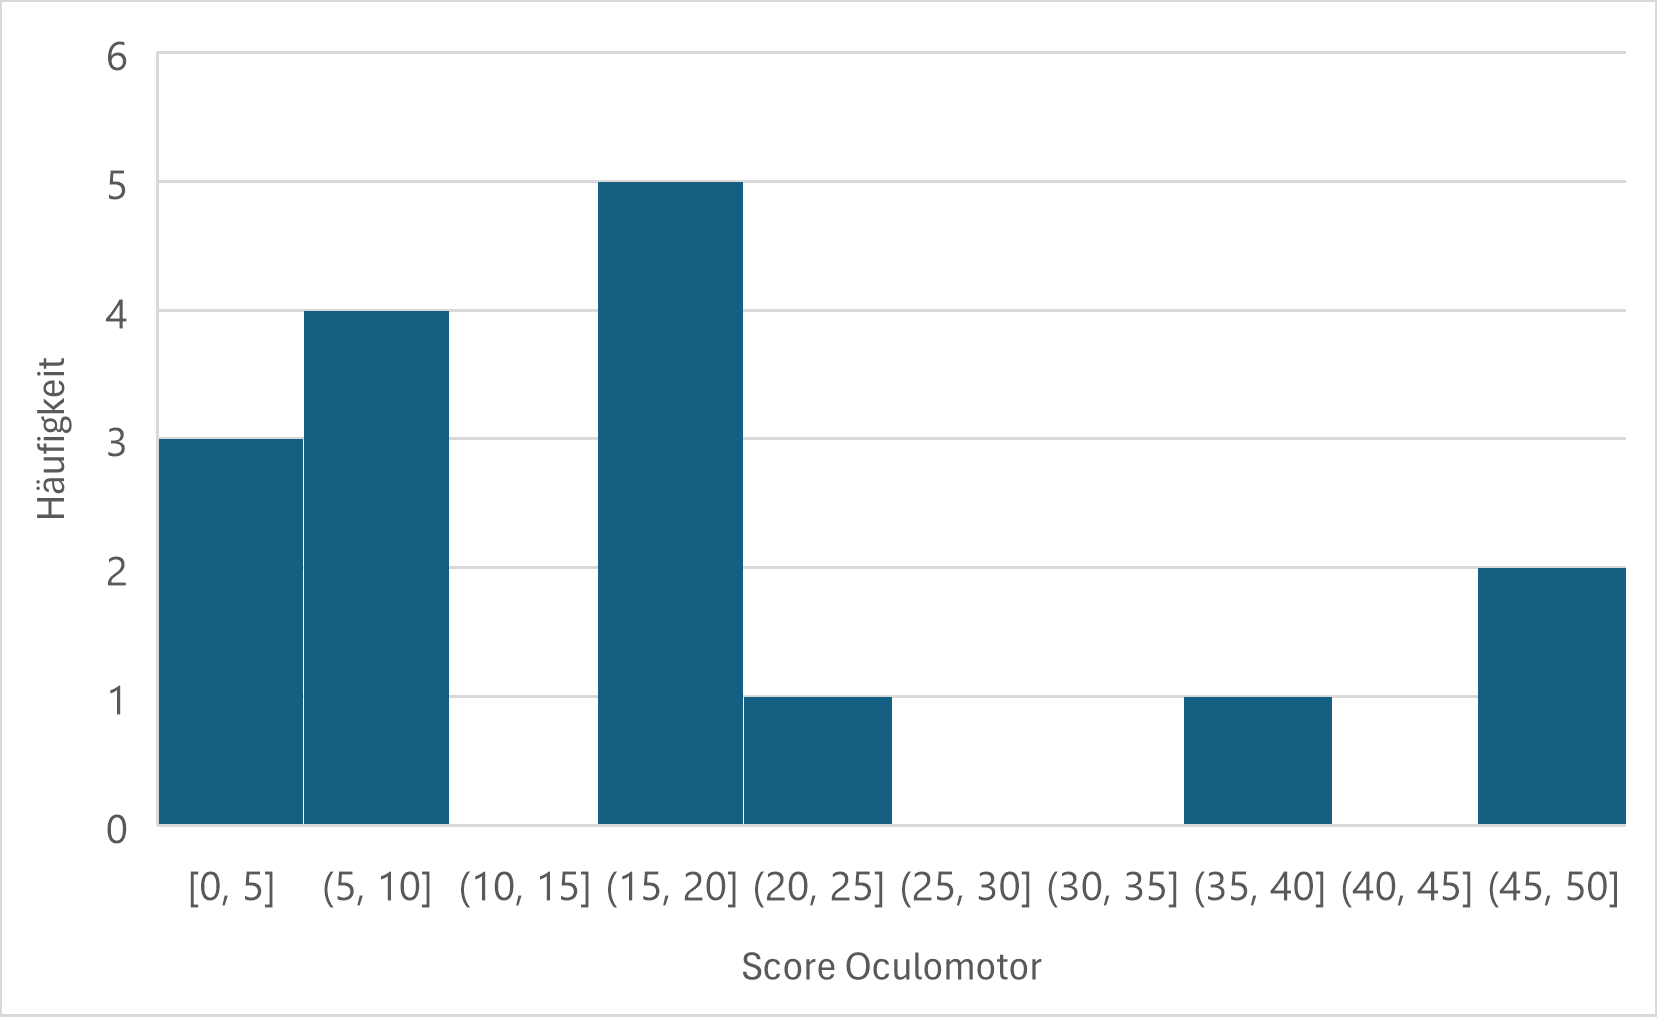
\includegraphics[width=0.99\textwidth]{images/Results/Histogramm-Oculomotor-Scale-Cartesian.png}
         \caption{Cartesian Scanning}
         \label{fig:histoOculomotorCartesian}
    \end{subfigure}
    \caption{Verteilung der Scores der SSQ Oculomotor Scale beider Interaktionsschnittstellen}
    \label{fig:histoOculomotor}
\end{figure}

In der Kategorie Oculomotor (vgl. \autoref{fig:histoOculomotor}) traten häufiger Symptome auf. Während beim Item Scanning sechs Personen keine bis nur sehr leichte Symptome (Score <10) aufwiesen, erreichten sieben Teilnehmende einen Score zwischen 15 und 35. Dies entspricht dem Auftreten von zwei oder mehr leichten oder mindestens einem moderaten Symptom. Drei Teilnehmende erreichten einen Score über 35, was auf das Auftreten mehrerer Symptome und mindestens einem Symptom in moderater Ausprägung hinwiest. Der Mittelwert der Scores dieser Kategorie liegt bei 18,476 (SD = 15,892) (vgl. \autoref{tab:tableErgebnisseSSQ}). Beim Cartesian Scanning zeigten sieben Personen keine bis leichte Symptome. Fünf Personen wiesen einen Score zwischen 15 und 20 auf. Vier Personen erreichten einen Score größer 20, wobei zwei Personen einen Score von über 45 erreichten. Der Mittelwert der Scores dieser Kategorie für das Cartesain Scnning liegt bei 16,108 (SD = 14,873) (vgl. \autoref{tab:tableErgebnisseSSQ}).

\begin{figure}
    \centering
    \begin{subfigure}{.5\textwidth}
        \centering
        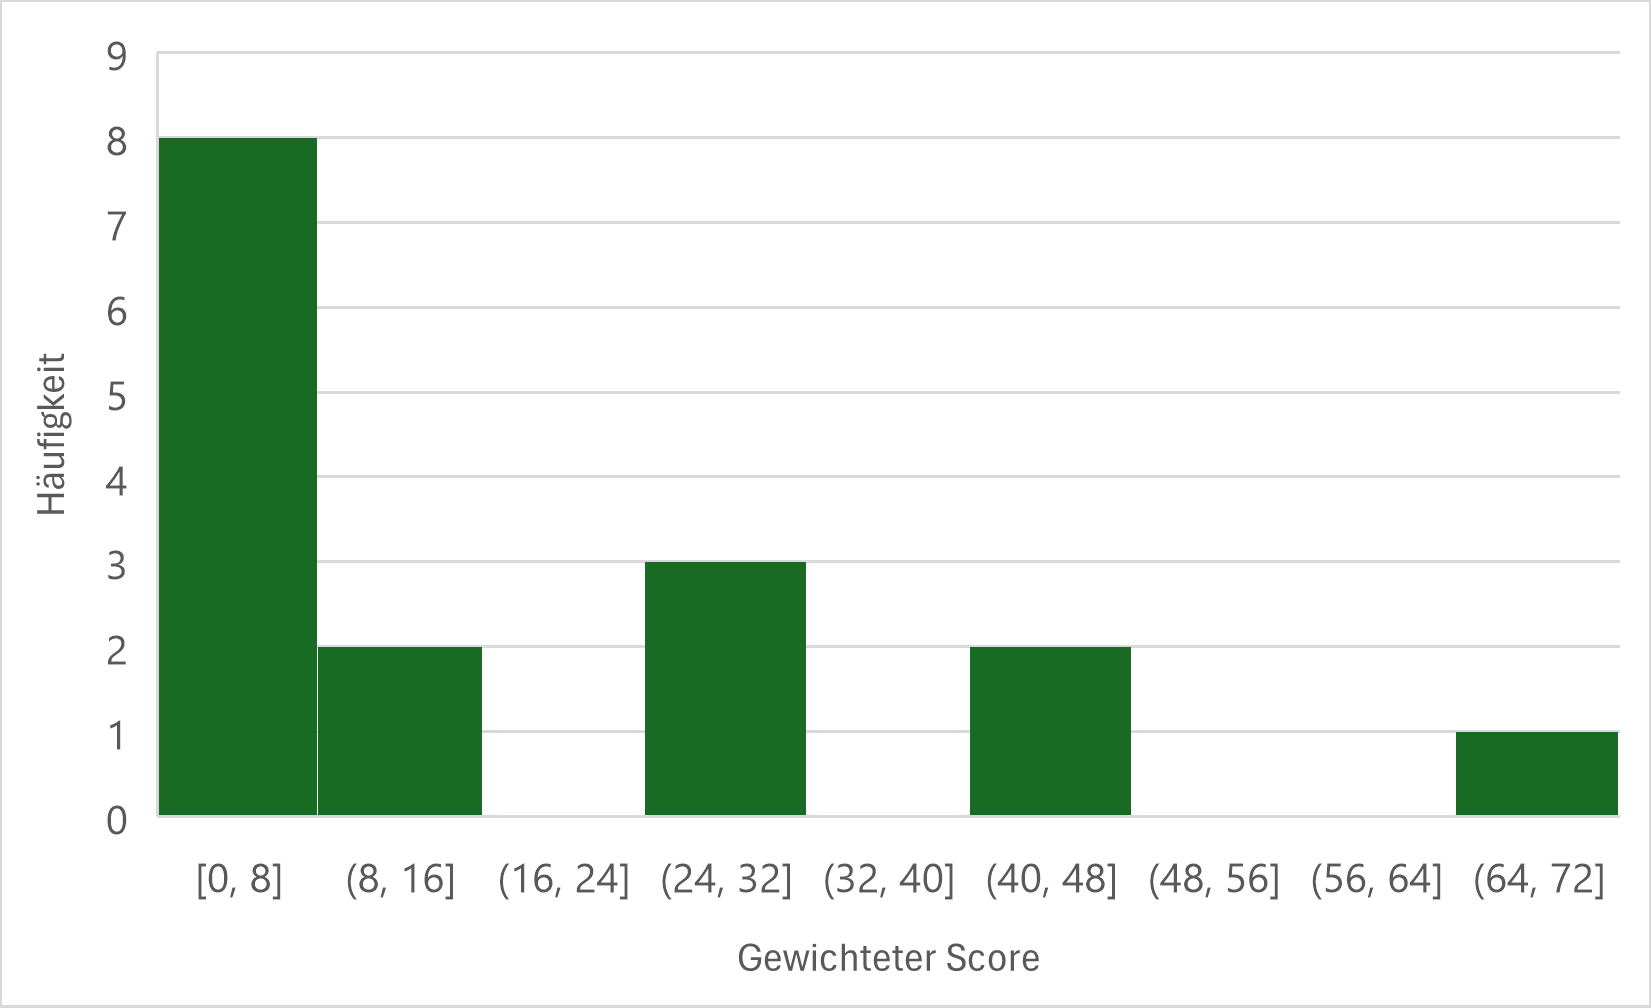
\includegraphics[width=0.99\textwidth]{images/Results/Histogramm-Disorientation-Scale-Item.png}
        \caption{Item Scanning}
        \label{fig:histoDisorientationItem}   
    \end{subfigure}%
    \begin{subfigure}{.5\textwidth}
        \centering
        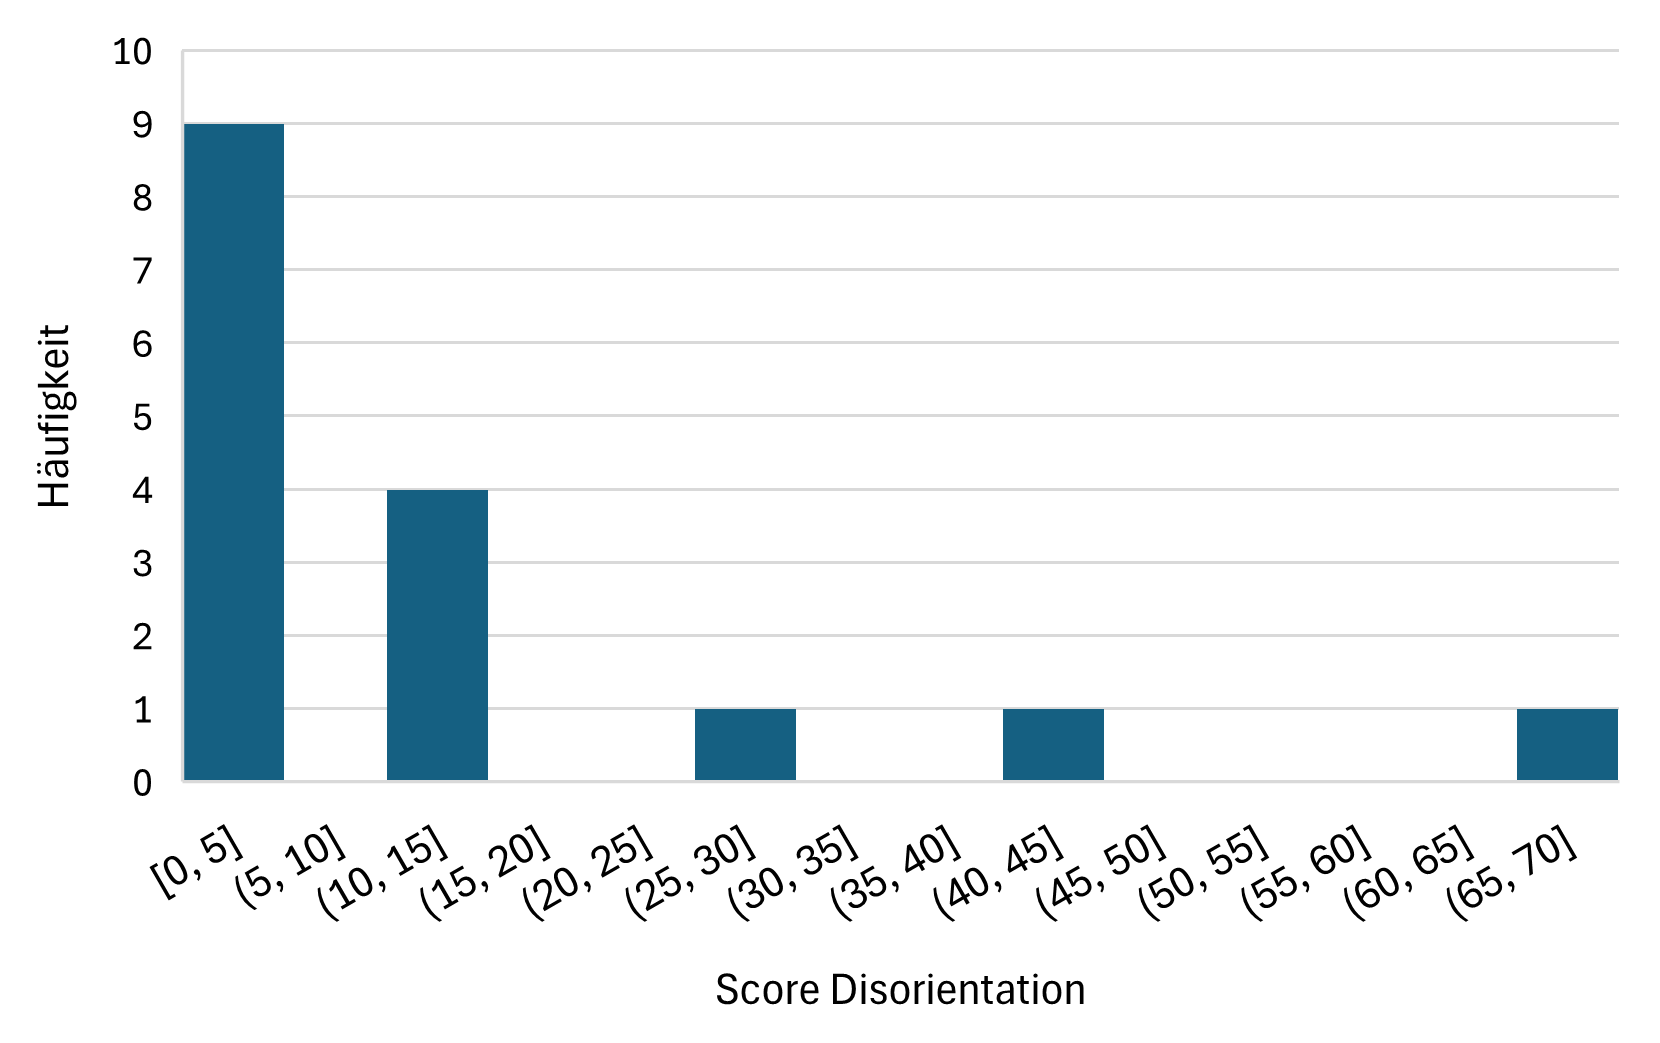
\includegraphics[width=0.99\textwidth]{images/Results/Histogramm-Disorientation-Scale-Cartesian.png}
         \caption{Cartesian Scanning}
         \label{fig:histoDisorientationCartesian}
    \end{subfigure}
    \caption{Verteilung der Scores der SSQ Disorientation Scale beider Interaktionsschnittstellen}
    \label{fig:histoDisorientation}
\end{figure}

In der Kategorie Desorientierung (vgl. \autoref{fig:histoDisorientation}) zeigten beim Item Scanning acht Personen keine Symptome. Zwei Teilnehmende erreichten einen Score zwischen 10 und 15. Sechs Personen erreichten einen Score über 25, wobei eine Person sogar einen Score größer 60 erreichte. Der Mittelwert der Scores dieser Kategorie für das Item Scnning liegt bei 16,530 (SD = 21,092) (vgl. \autoref{tab:tableErgebnisseSSQ}). Beim Cartesian Scanning blieben neun Personen symptomfrei, während vier Personen einen Score zwischen 10 und 15 erreichten. Nur drei Personen erreichten einen Score über 25, wobei eine Person soagr einen Score von 65 überschritt. Der Mittelwert der Scores dieser Kategorie liegt bei 12,180 (SD = 19,604) (vgl. \autoref{tab:tableErgebnisseSSQ}).

\subsection{Ablenkung durch die Interaktionsschnittstellen}

Die Ergebnisse zur Ablenkung bzw. Presence wurden anhand von drei Fragen erhoben, deren Mittelwerte für beide Schnittstellen in der \autoref{fig:presence} dargestellt sind.

\begin{figure}[tbh]
    \centering
    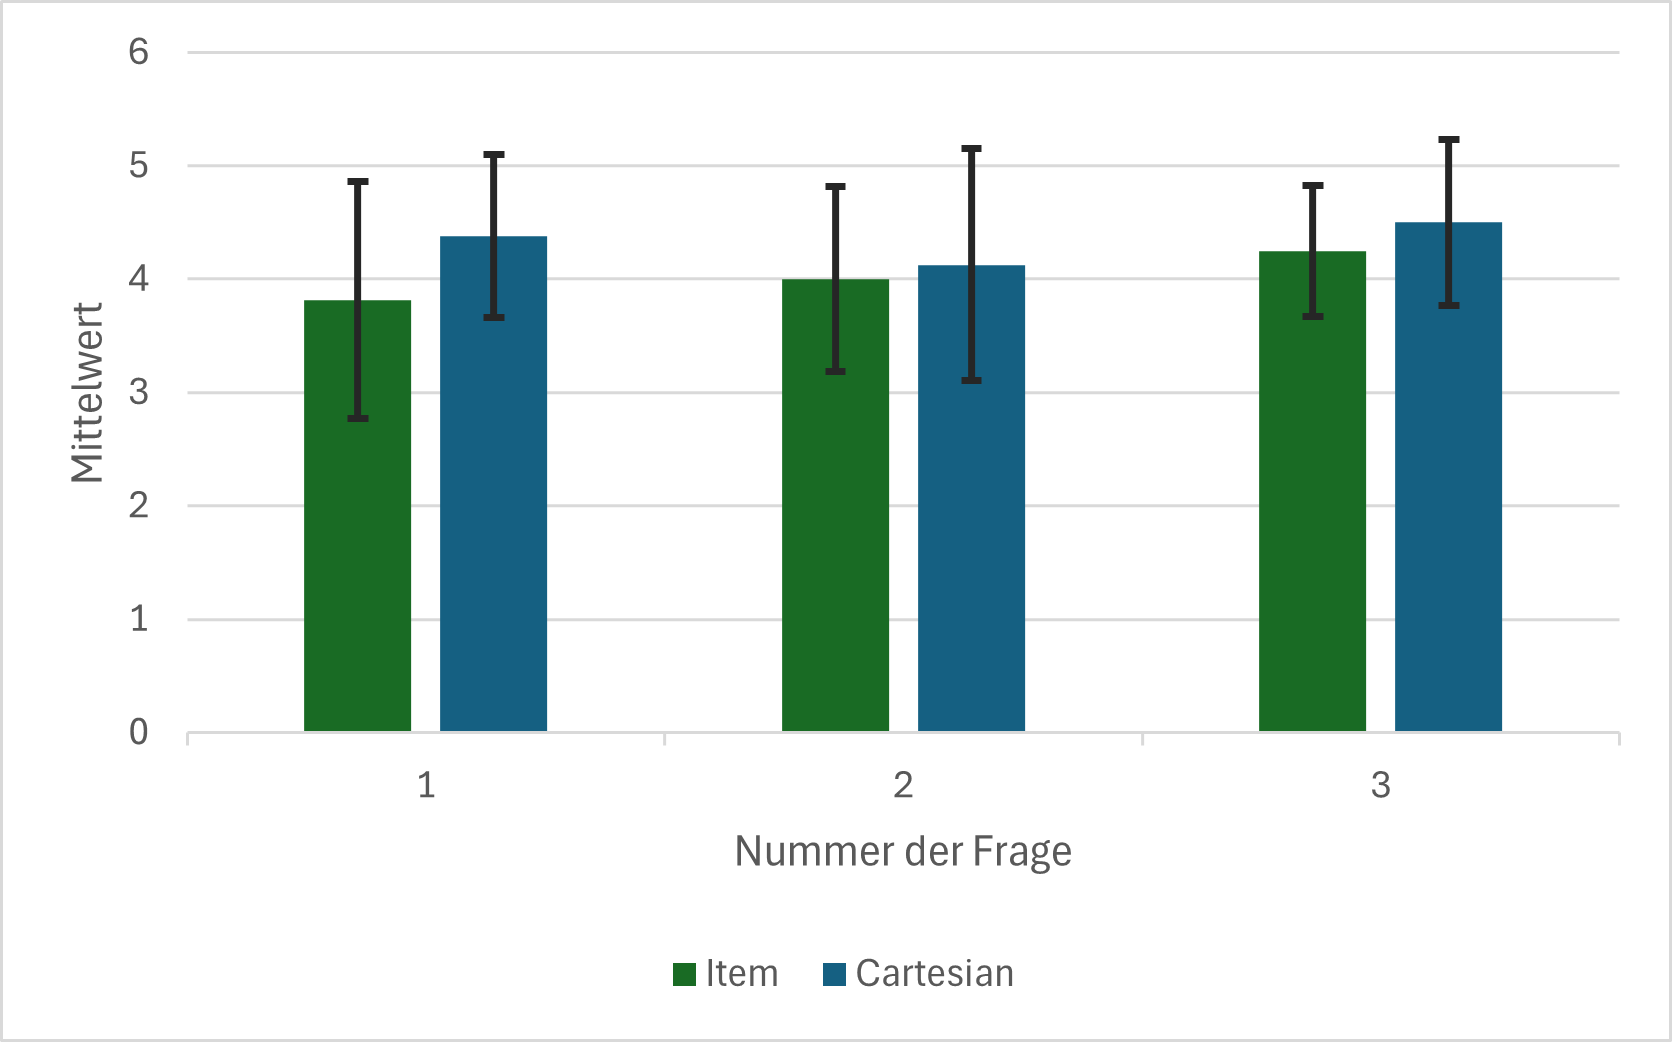
\includegraphics{images/Results/Fragen-zur-Presence-Ablenkung.png}
    \caption{Ergebnisse der Fragen zur Ablenkung durch die Interaktionsschnittstellen}
    \label{fig:presence}
\end{figure}

\textit{Frage 1:} Wie sehr warst Du in die Erfahrung der virtuellen Umgebung involviert?
Die Bewertungen für das Item Scanning zeigen einen Mittelwert von 3,813 (SD = 1,047). Für das Cartesian Scanning liegt der Mittelwert bei 4,375 (SD = 0,719).

\textit{Frage 2:} Wie gut konntest Du Dich auf die zugewiesenen Aufgaben oder erforderlichen Tätigkeiten konzentrieren und nicht auf die Mechanismen, die zur Ausführung dieser Aufgaben oder Tätigkeiten genutzt werden?
Bei dieser Frage erreicht das Item Scanning einen Mittelwert von 4,000 (SD = 0,817), während das Cartesian Scanning einen Mittelwert von 4,125 (SD = 1,025) aufweist.

\textit{Frage 3:} Wie gut konntest Du Dich auf den Inhalt und die visuellen Darstellungen in der Szene konzentrieren?
Die Ergebnisse für das Item Scanning zeigen einen Mittelwert von 4,250 (SD = 0,577). Beim Cartesian Scanning wird ein Mittelwert von 4,500 (SD = 0,730) erzielt.

\subsection{Geschwindigkeit und Effizienz}

Die durchschnittlichen Zeiten für die Durchführung der Evaluationsabschnitte zeigen Unterschiede zwischen den beiden Schnittstellen, dargestellt in \autoref{fig:zeit} Beim Item Scanning benötigten die Teilnehmenden im technischen Abschnitt durchschnittlich 6 Minuten und 42 Sekunden (SD = 1 Minute und 26 Sekunden). Im inhaltsbasierten Abschnitt betrug die benötigte Zeit durchschnittlich 5 Minuten und 35 Sekunden (SD = 1 Minute und 43 Sekunden).
Beim Cartesian Scanning hingegen betrug die für den technischen Abschnitt benötigte Zeit durchschnittlich 8 Minuten und 5 Sekunden (SD = 1 Minute und 41 Sekunden). Für den inhaltsbasierten Abschnitt wurden durchschnittlich 8 Minuten 50 Sekunden benötigt (SD = 2 Minuten 52 Sekunden).

\begin{figure}[tbh]
    \centering
    \includegraphics{images/Results/Benötigte-Zeit-Evaluationsabschnitte.png}
    \caption{Benötigte Zeit zum Durchlaufen der Evaluationsabschnitte}
    \label{fig:zeit}
\end{figure}

Für die Auswertung der Geschwindigkeiten wurden die Interaktionsgeschwindigkeiten aus den Log-Files pro Person zusammengefasst. Daraus wurden Mittelwerte, Varianzen und Spannweiten berechnet, sowohl getrennt für jeden Evaluationsabschnitt als auch zusammengefasst für beide Abschnitte. Die Ergebnisse sind in der \autoref{tab:InteraktionsgeschwindigkeitenTable} aufgezigt sowie in der \autoref{fig:Interaktionsgeschwindigkeiten} visualisiert. 

Beim Item Scanning beträgt die durchschnittliche Interaktionsgeschwindigkeit im technischen Abschnitt 4.617s (Varianz = 0.381; Spannweite = 2.064). Dagegen ist die Interaktionsgeschwindigkeit im inhaltsbasierten Abschnitt mit 2,927s kürzer (Varianz = 0,522; Spannweite = 2,274). Über beide Abschnitte hinweg ergibt sich eine durchschnittliche Interaktionsgeschwindigkeit von 3,862s (Varianz = 0,293; Spannweite = 1,917).
Beim Cartesian Scanning werden im technischen Abschnitt durchschnittlich 8,733s (Varianz = 1,733; Spannweite = 4,840) zur Interaktion benötigt. Im inhaltsbasierten Abschnitt beträgt die mittlere Interaktionsgeschwindigkeit 7,404s (Varianz = 5,616; Spannweite = 7,340). Über beide Abschnitte hinweg ergibt sich eine Interaktionsgeschwindigkeit von 8,004s (Varianz = 3,383; Spannweite = 5,603).

\begin{table}[tbh]
    \centering
    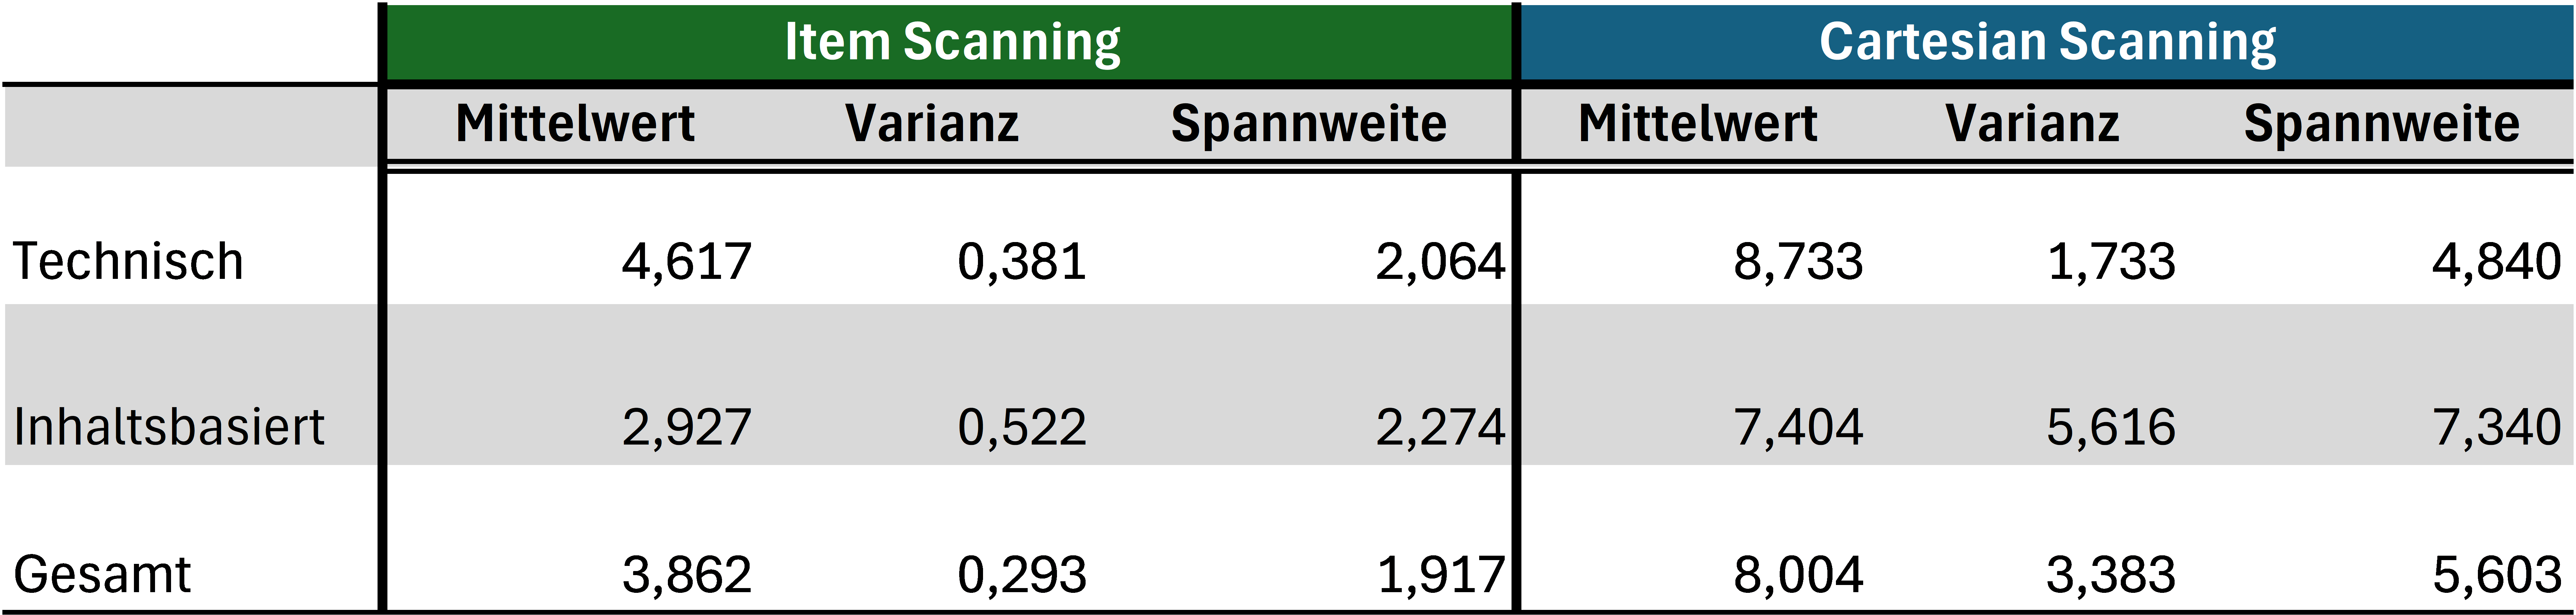
\includegraphics[width=0.95\textwidth]{images/Results/Interaktionsgeschwindigkeiten-Table.png}
    \caption{Interaktionsgeschwindigkeiten beider Interaktionsschnittstellen nach Evalauationsabschnitt}
    \label{tab:InteraktionsgeschwindigkeitenTable}
\end{table}

\begin{figure}[tbh]
    \centering
    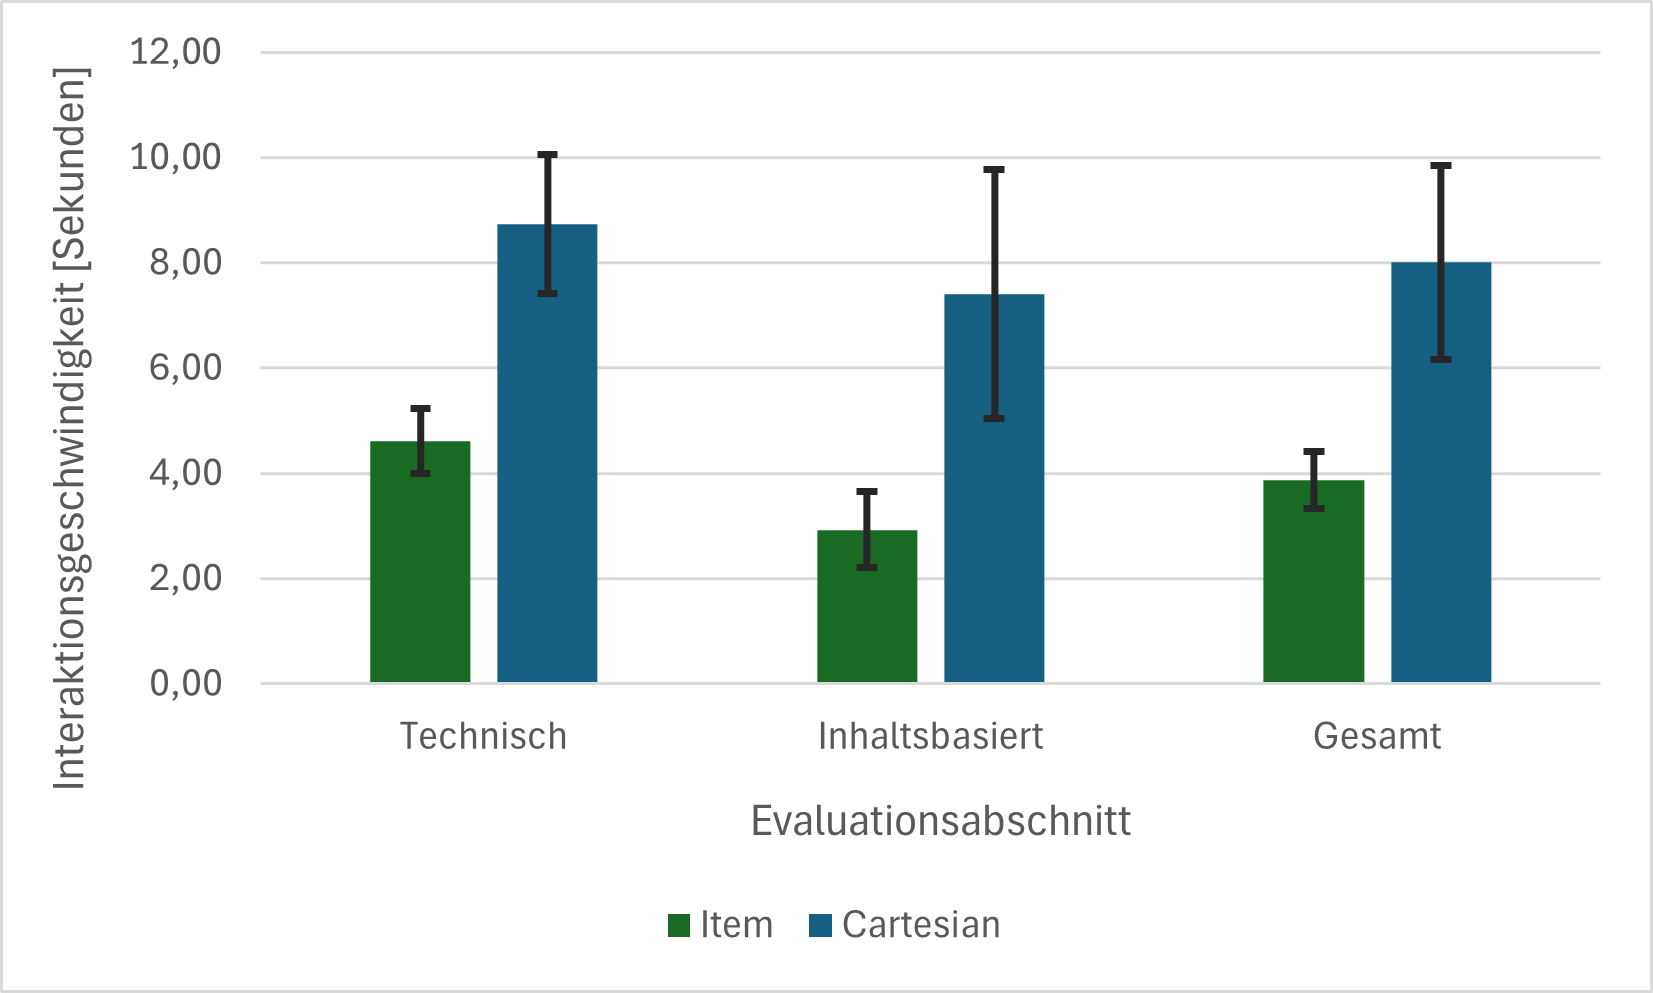
\includegraphics[width=0.75\textwidth]{images/Results/Interaktionsgeschwindigkeiten.png}
    \caption{Darstellung der mittleren Interaktionsgeschwindigkeiten beider Interaktionsschnittstellen nach Evalauationsabschnitt}
    \label{fig:Interaktionsgeschwindigkeiten}
\end{figure}

Um die Veränderung der Interaktionsgeschwindigkeit über die Zeit bzw. über die Anzahl der durchgeführten Interaktionen zu untersuchen, wurde eine lineare Regressionsanalyse durchgeführt und anschließend die Korrelation zwischen den beiden Variablen berechnet. Die Ergebnisse werden in \autoref{tab:RegressionskoeffizientenTable} aufgezeigt. Der Regressionskoeffizient beschreibt die durchschnittliche Veränderung der Interaktionszeit in Abhängigkeit von der Anzahl der bereits durchgeführten Interaktionen. Der Korrelationskoeffizient gibt an, wie eng der Zusammenhang zwischen den Variablen ist. 
Beim Item Scanning ergibt sich für den technischen Abschnitt ein mittlerer Regressionskoeffizient von -0,839 (Varianz = 0,503) bei einem Korrelationskoeffizienten von -0,219. Im inhaltsbasierten Abschnitt beträgt der mittlere Regressionskoeffizient -0,391 (Varianz = 0,754) bei einem Korrelationskoeffizienten von -0,066. Über beide Abschnitte hinweg ergibt sich ein mittlerer Regressionskoeffizient von -2,539 (Varianz = 1,105) und ein Korrelationskoeffizient von -0,263.
Beim Cartesian Scanning ergibt sich für den technischen Abschnitt ein durchschnittlicher Regressionskoeffizient von 0,180 (Varianz = 0,326) mit einem Korrelationskoeffizienten von 0,038. Im inhaltsbasierten Abschnitt beträgt der Regressionskoeffizient 0,241 (Varianz = 1,177) und der Korrelationskoeffizient -0,019. Über beide Abschnitte hinweg beträgt der Regressionskoeffizient -0,492 (Varianz = 1,461) und der Korrelationskoeffizient -0,085.

\begin{table}[tbh]
    \centering
    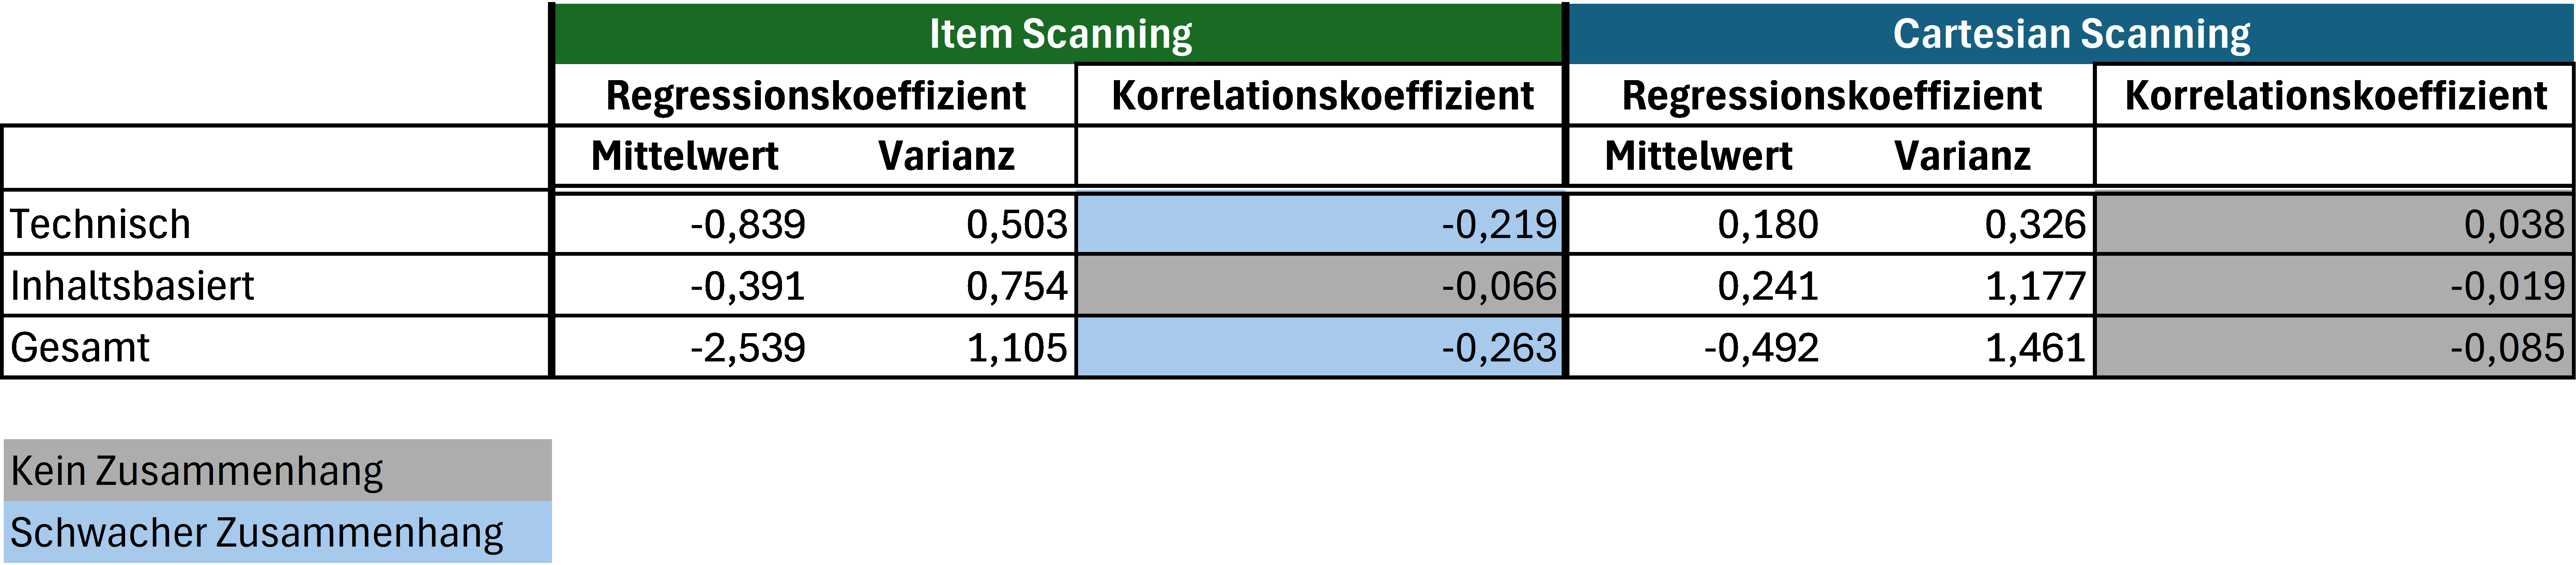
\includegraphics[width=0.95\textwidth]{images/Results/Regressionskoeffizienten-Korrelation-Table-Lernkurve-Geschwindigkeit.png}
    \caption{Ergebnisse der linearen Regressionsanalyse}
    \label{tab:RegressionskoeffizientenTable}
\end{table}

Neben der Interaktionsgeschwindigkeit wurde auch die Anzahl der benötigten Scanning Zyklen pro Interaktion im Log-File erfasst. Die \autoref{tab:zyklen} zeigt die Ergebnisse bezüglich der Zyklen für das Item Scanning. Im technischen Abschnitt wurden durchschnittlich 1,542 Zyklen pro Eingabe benötigt (Varianz = 0,007; Spannweite = 0,332). Im inhaltsbasierten Abschnitt hingegen lag der Mittelwert bei 1,423 (Varianz = 0,021; Spannweite = 0,481).

%Auch für das Cartesian Scanning wurde die Anzahl der benötigten Durchläufe der Scaninng-Linien ausgegeben. hier noch die Erklärung ergänzen! 

\begin{table}[tbh]
    \centering
    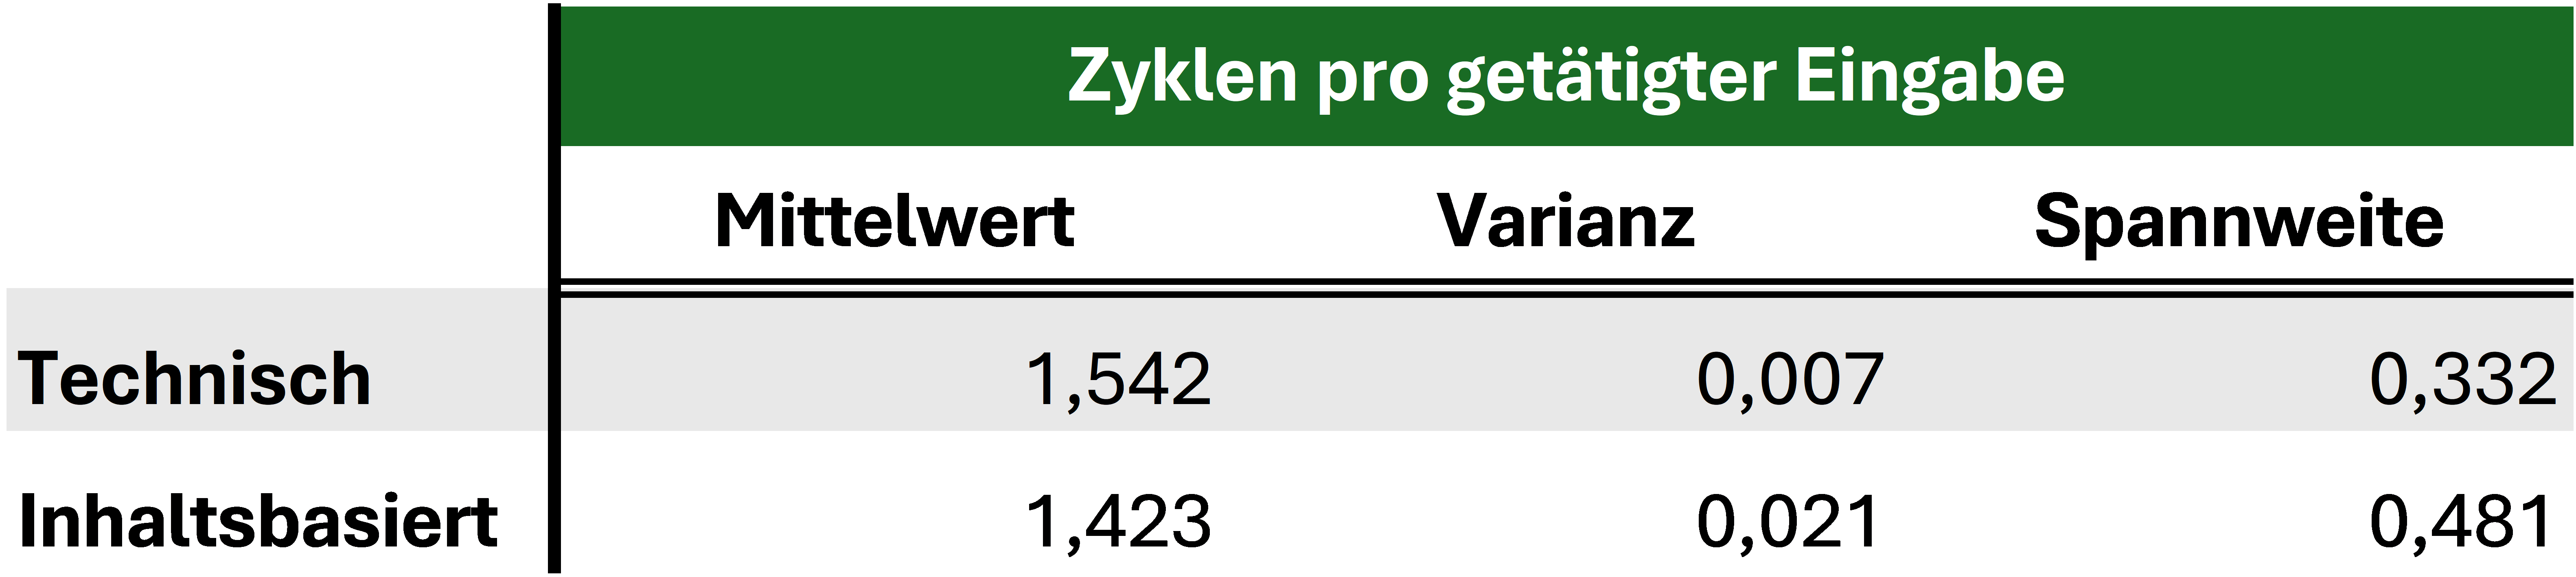
\includegraphics{images/Results/Zyklen-Item.png}
    \caption{Benötigte Scanning-Zyklen pro Interaktion beim Item Scanning}
    \label{tab:zyklen}
\end{table}

\subsection{Robustheit}

In beiden Evalauationsabschnitten wurden die aufgetretenen Fehler im Evaluationsprotokoll erfasst. Als Fehler werden in diesem Zusammenhang Eingaben verstanden, die nicht zum gewünschten Ergebnis geführt haben. 

Die Ergebnisse des Item Scannings sind in \autoref{fig:anzahlFehlerItem} dargestellt. Im technischen Abschnitt (vgl. \autoref{fig:anzahlFehlerItemTechnisch}) traten bei der Mehrheit der Teilnehmenden Fehler auf. Nur drei Personen konnten den Abschnitt ohne Fehler abschließen. Sieben Personen machten einen Fehler, zwei Personen machten jeweils drei Fehler. Eine Person hat fünf Fehler gemacht. Somit wurden in diesem Abschnitt über alle Testpersonen hinweg insgesamt 18 Fehler erfasst.
Im inhaltsbasierten Abschnitt (vgl. \autoref{fig:anzahlFehlerItemInhalt}) haben sechs Personen keinen Fehler gemacht, während weitere sechs Personen jeweils einen Fehler machten. Vier Personen machten zwei Fehler. Keine Testperson hat in diesem Abschnitt mehr als zwei Fehler gemacht. Insgesamt wurden in diesem Abschnitt 14 Fehler verzeichnet.

\begin{figure}[tbh]
    \centering
    \begin{subfigure}{.5\textwidth}
        \centering
        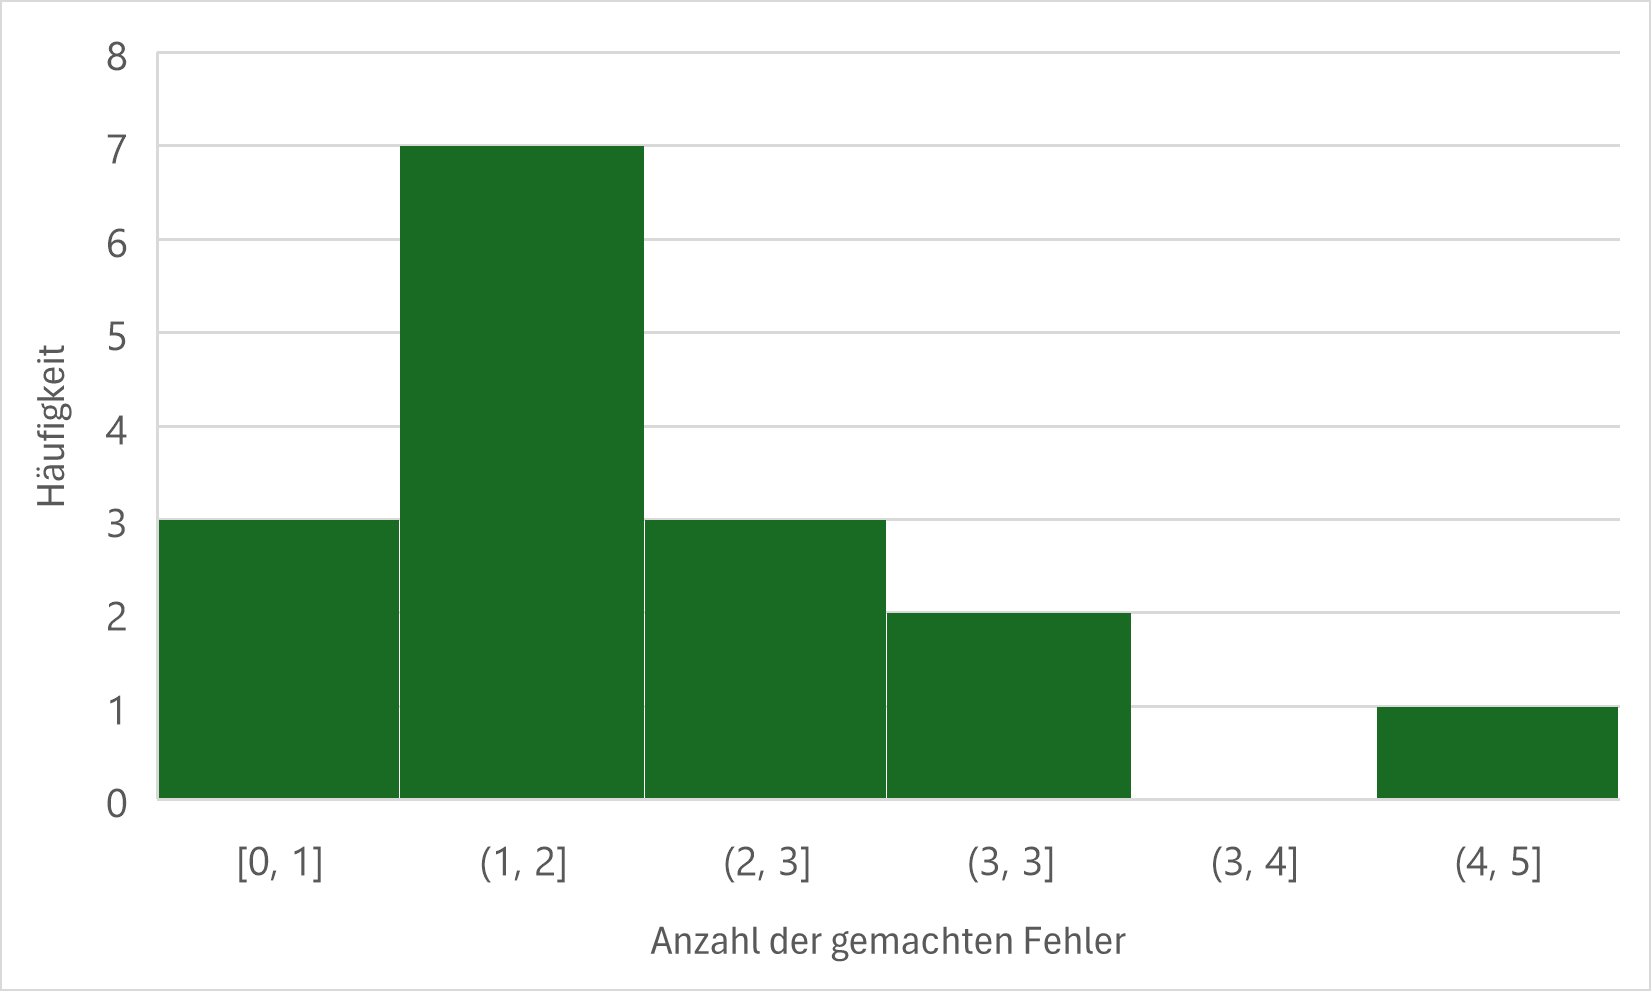
\includegraphics[width=0.95\textwidth]{images/Results/Histogramm-Anzahl-Fehler-technisch-item.png}
        \caption{Technischer Abschnitt}
        \label{fig:anzahlFehlerItemTechnisch}
    \end{subfigure}%
    \begin{subfigure}{.5\textwidth}
        \centering
        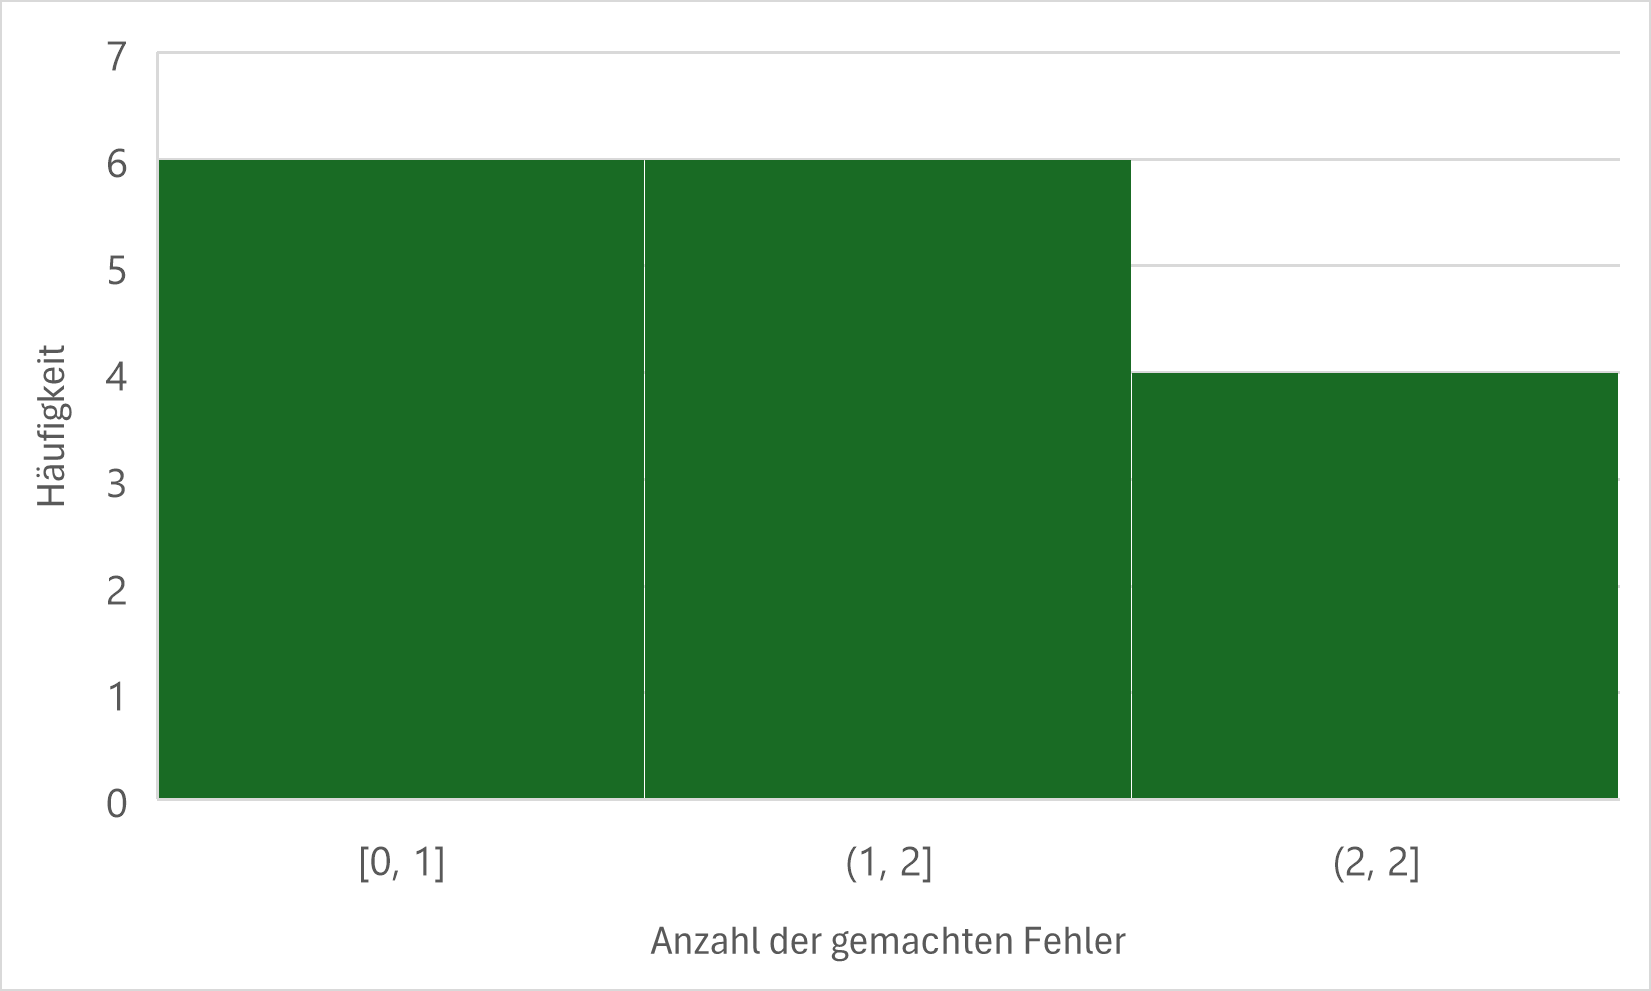
\includegraphics[width=0.95\textwidth]{images/Results/Histogramm-Anzahl-Fehler-inhalt-item.png}
        \caption{Inhaltsbasierter Abschnitt}
        \label{fig:anzahlFehlerItemInhalt}
   \end{subfigure}
   \caption{Häufigkeiten der Anzahl gemachter Fehler im Item Scanning}
   \label{fig:anzahlFehlerItem}
\end{figure}
\

Im Evaluationsprotokoll wurde für jeden aufgetretenen Fehler der jeweilige Grund vermerkt. Die beim Item Scanning aufgetretenen Gründe sind in \autoref{fig:gründeFehlerItem} aufgeführt. Es ist zu erkennen, dass die meisten Fehler auf Timing-Probleme zurückzuführen sind. Das bedeutet, dass Eingaben etwas zu früh oder etwas zu spät erfolgten und dadurch versehentlich das vorherige oder nachfolgende Item in der Scanning-Reihenfolge anstelle des Zielobjekts ausgewählt wurde. Zu späte Eingaben traten insbesondere bei der Navigation auf. Derartige Fehler traten bei 13 der 16 Testpersonen auf. Im technischen Abschnitt der Evaluation traten zudem Fehler auf, die auf Verständnisprobleme zurückzuführen sind. Vier Teilnehmenden war das Prinzip bzw. die Aufgabe zu Beginn nicht ganz klar, wodurch es zu fehlerhaften Eingaben kam. 

\begin{figure}[tbh]
    \centering
    \includegraphics{images/Results/Gründe-Fehler-Item.png}
    \caption{Gründe für Fehler beim Item Scanning}
    \label{fig:gründeFehlerItem}
\end{figure}

Die Ergebnisse des Cartesian Scanning sind in \autoref{fig:anzahlFehlerCartesian} dargestellt.
Den technischen Abschnitt (vgl. \autoref{fig:anzahlFehlerCartesianTechnisch}) konnten sieben Personen fehlerfrei abschließen. Drei Personen machten jeweils einen oder zwei Fehler, während jeweils eine Person drei, vier oder sechs Fehler machte. Insgesamt wurden in diesem Abschnitt über alle Testpersonen hinweg 22 Fehler erfasst. 
Im inhaltsbasierten Abschnitt (vgl. \autoref{fig:anzahlFehlerCartesianInhalt}) blieb die Hälfte der Testpersonen fehlerfrei. Fünf Personen machten jeweils einen Fehler, eine Person drei, eine Person vier und eine Person acht Fehler. Die Gesamtzahl der Fehler beträgt hier somit 20.

\begin{figure}
    \centering
    \begin{subfigure}{.5\textwidth}
        \centering
        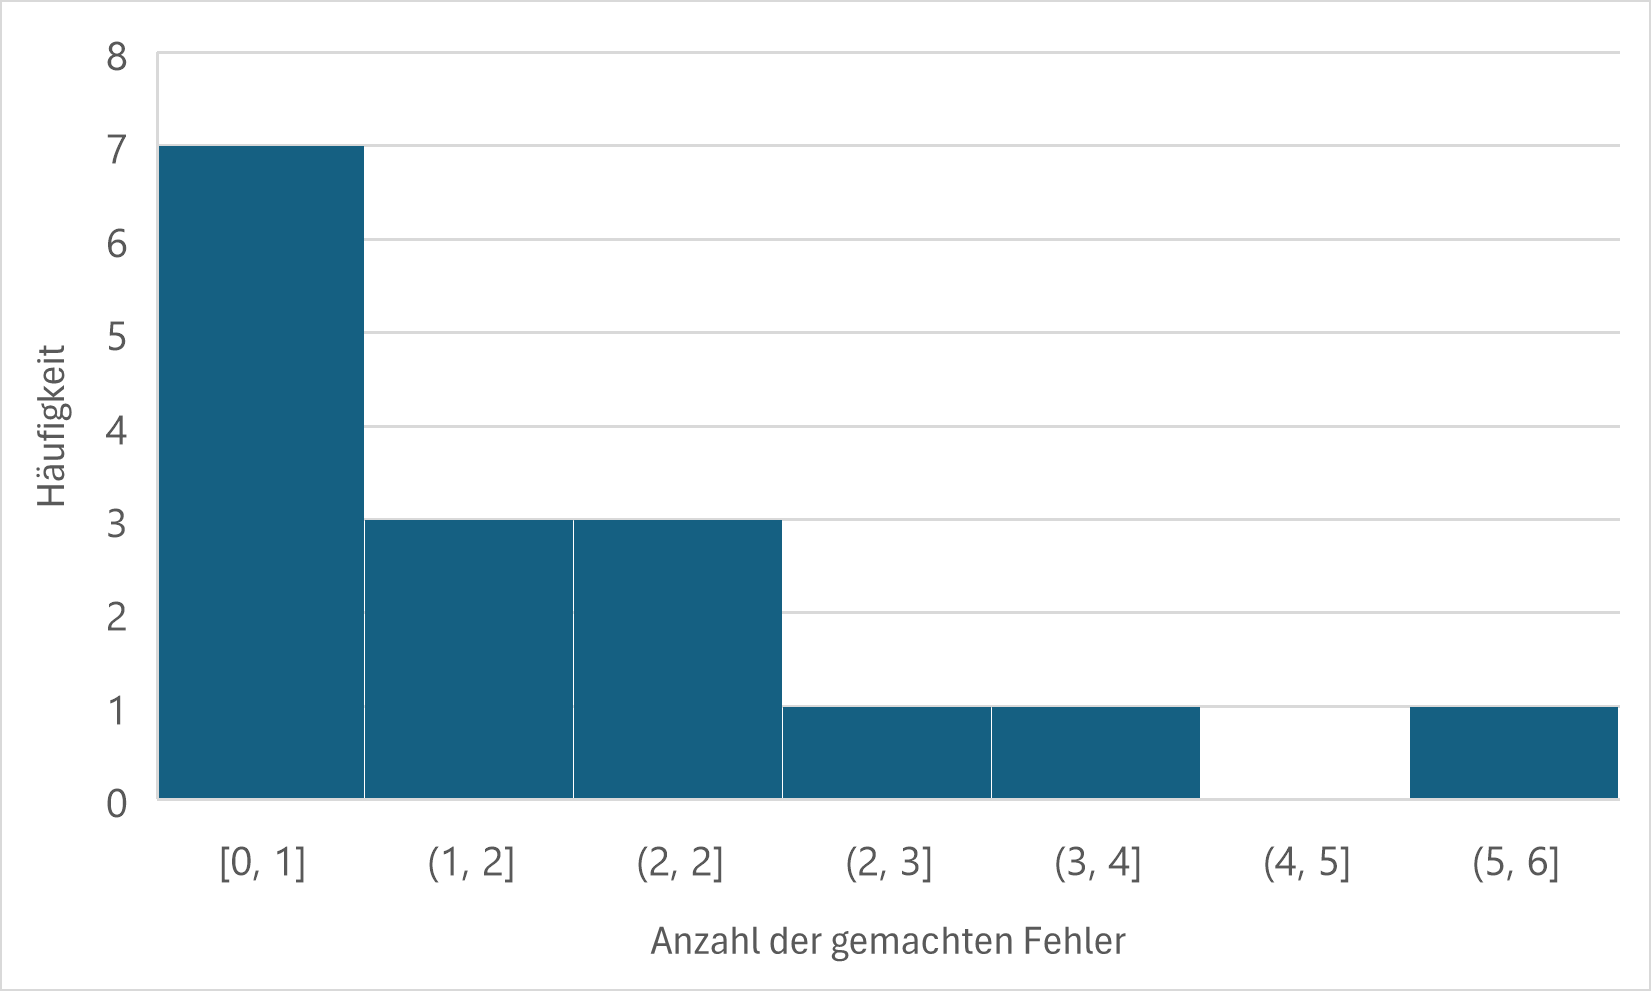
\includegraphics[width=0.95\textwidth]{images/Results/Histogramm-Anzahl-Fehler-technisch-cartesian.png}
        \caption{Technischer Abschnitt}
        \label{fig:anzahlFehlerCartesianTechnisch}
    \end{subfigure}%
    \begin{subfigure}{.5\textwidth}
        \centering
        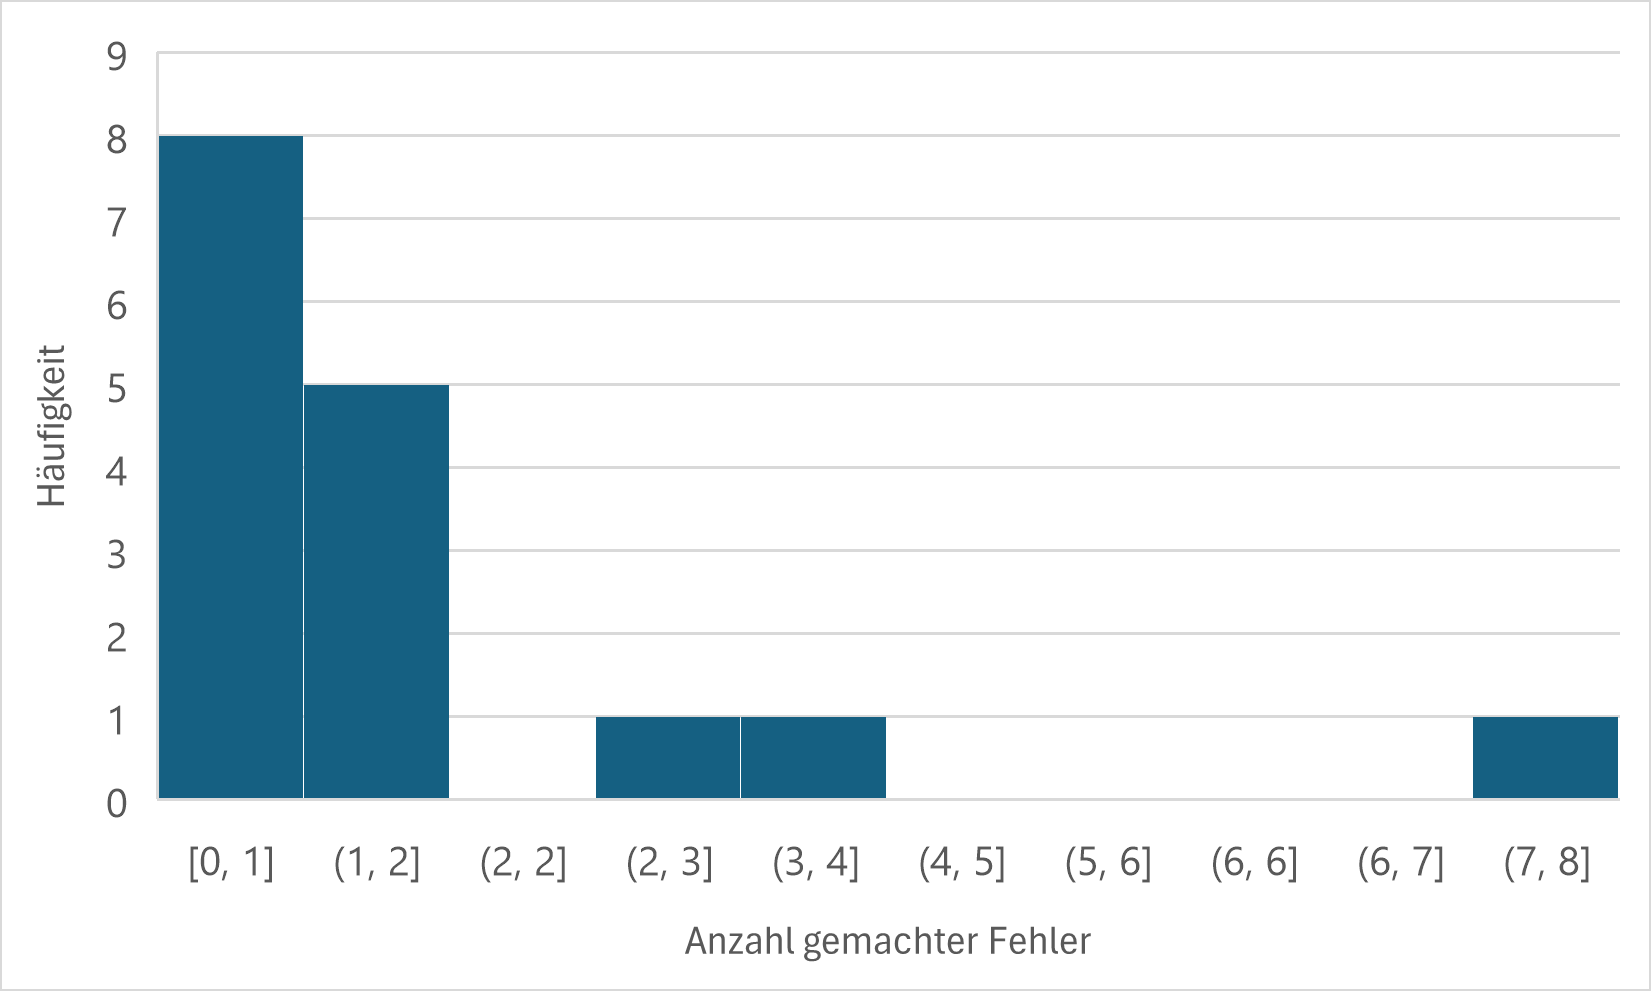
\includegraphics[width=0.95\textwidth]{images/Results/Histogramm-Anzahl-Fehler-inhalt-cartesian.png}
        \caption{Inhaltsbasierter Abschnitt}
        \label{fig:anzahlFehlerCartesianInhalt}
    \end{subfigure}
    \caption{Häufigkeiten der Anzahl gemachter Fehler beim Cartesian Scanning}
    \label{fig:anzahlFehlerCartesian}
\end{figure}

Die Gründe für Fehler beim Cartesian Scanning sind in \autoref{fig:gründeFehlerCartesian} dargestellt. Es ist zu erkennen, dass neun Personen versehentlich das HUD anstelle des beabsichtigten Objekts ausgewählt haben. Fünf Personen vergaßen den Moduswechsel, was dazu führte, dass statt einer Selektion weitere Navigationsschritte durchgeführt wurden. Drei Personen hatten Probleme beim Schließen von Bildern, da sie den Schließen-Button nicht wählen konnten. Eine Person hielt den Schalter für den Moduswechsel nicht lange genug gedrückt, sodass der Wechsel nicht ausgelöst wurde und weitere Navigationsschritte statt der gewünschten Selektion ausgeführt wurden. Eine Person selektierte versehentlich einen Wegpunkt, der hinter einem geöffneten Bild lag, obwohl eine leere Eingabe beabsichtigt war. 

\begin{figure}[tbh]
    \centering
    \includegraphics[width=0.95\textwidth]{images/Results/Gründe-Fehler-Cartesian.png}
    \caption{Gründe für Fehler beim Cartesian Scanning}
    \label{fig:gründeFehlerCartesian}
\end{figure}

Beim Cartesian Scanning wurde zusätzlich die Häufigkeit von leeren Eingaben zur Korrektur von Fehlern, wie z. B. das Setzen der ersten Scanlinie an der falschen Position oder das Vergessen des Wechsels in den Navigationsmodus, erfasst. Die Ergebnisse sind in \autoref{tab:leereEingaben} dargestellt. 
Im technischen Abschnitt beträgt die durchschnittliche Anzahl leerer Eingaben 1.000 (Varianz = 2.933; Spannweite = 7.000). Im inhaltsbasierten Abschnitt liegt der Mittelwert mit 1.750 (Varianz = 6.200; Spannweite = 10.000) etwas höher.

\begin{table}[tbh]
    \centering
    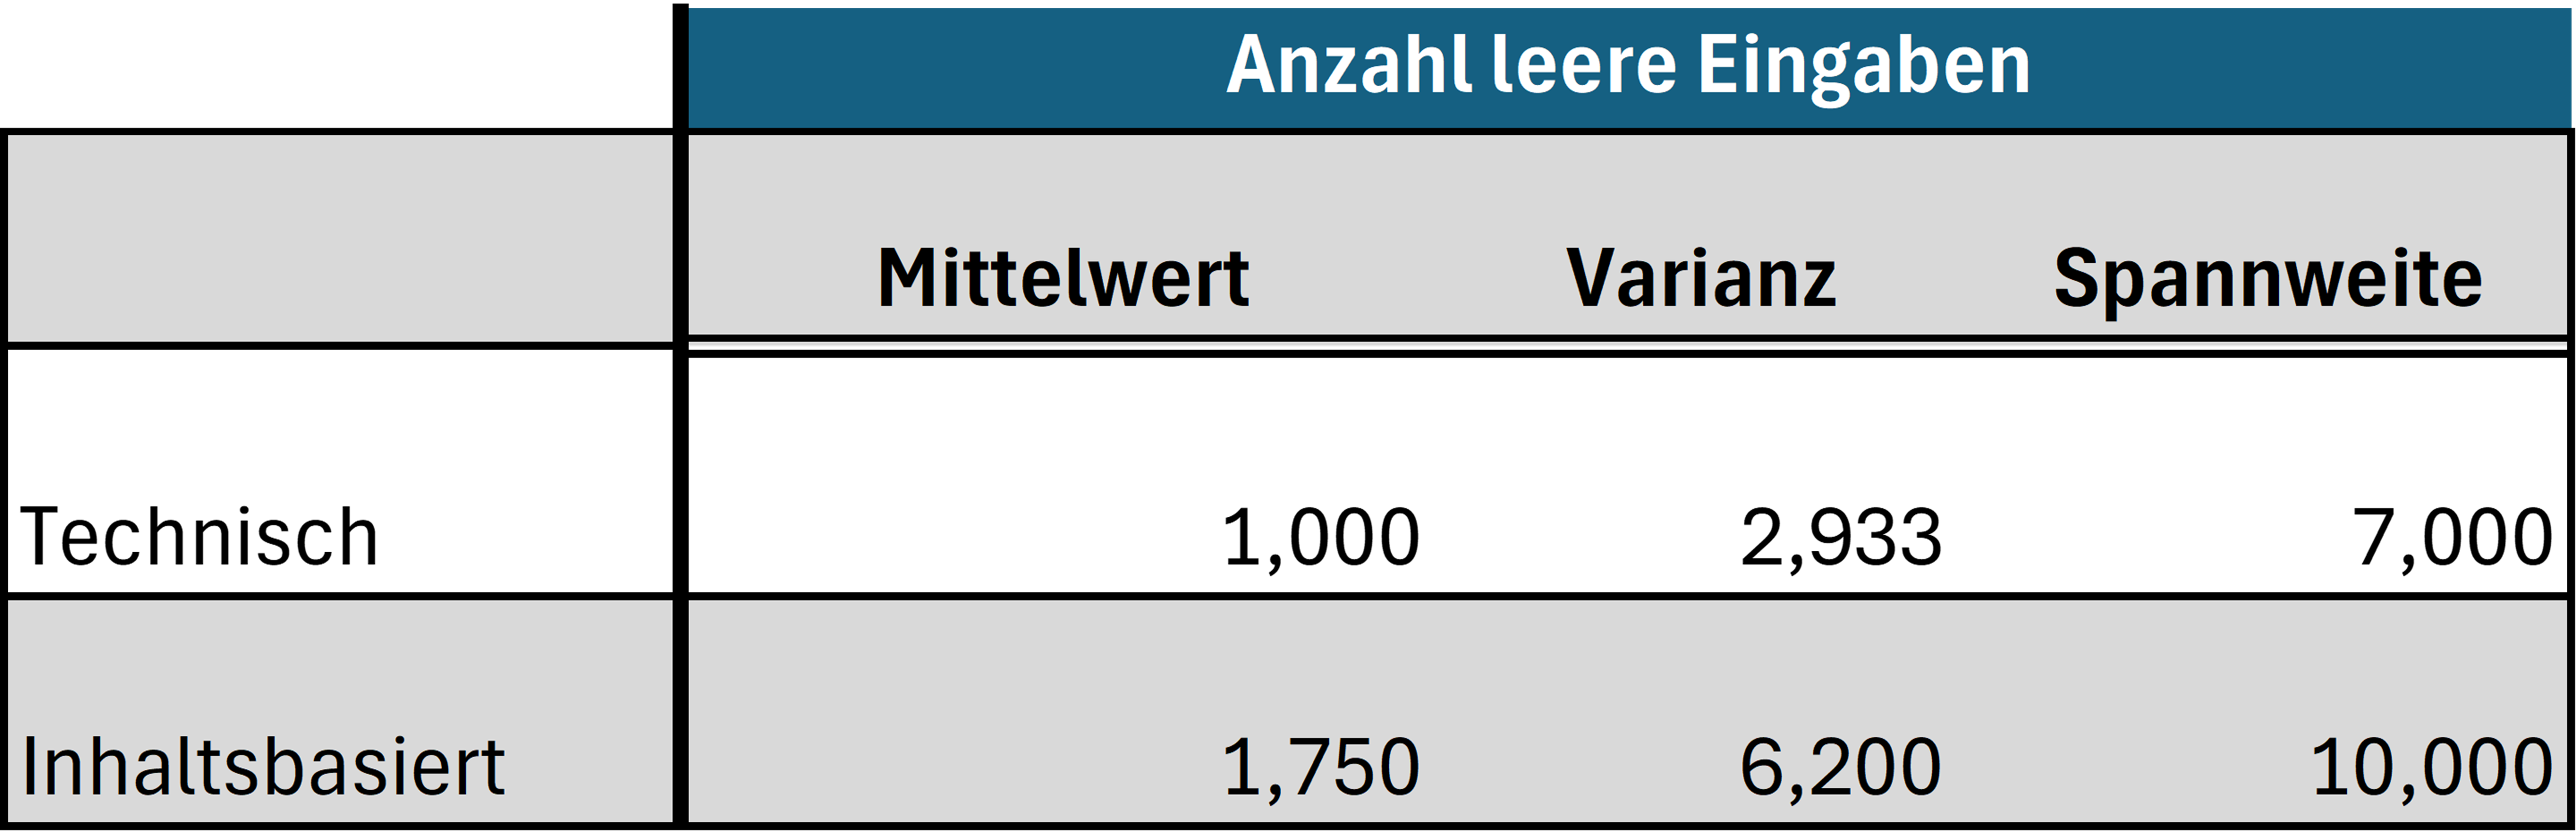
\includegraphics{images/Results/leereEingaben.png}
    \caption{Leere Eingaben beim Cartesian Scanning nach Evaluationsabschnitt}
    \label{tab:leereEingaben}
\end{table}

\subsection{Korrelationen und Zusammenhänge}

Neben der getrennten Auswertung der Ergebnisse der einzelnen Variablen und Faktoren wurden Korrelationsanalysen durchgeführt, um Zusammenhänge zwischen den Variablen zu untersuchen.

Zunächst wurde für das Cartesian Scanning untersucht, ob die Position der ausgewählten Objekte im Sichtfeld (x- und y-Koordinaten) einen signifikanten Einfluss auf die Interaktionsgeschwindigkeit hat. Die Ergebnisse sind in \autoref{tab:tableKorrPosGeschwindigkeit} zusammengefasst und in \autoref{fig:bubbleKorrPosGeschwindigkeit} visualisiert. 

\begin{table}[tbh]
    \centering
    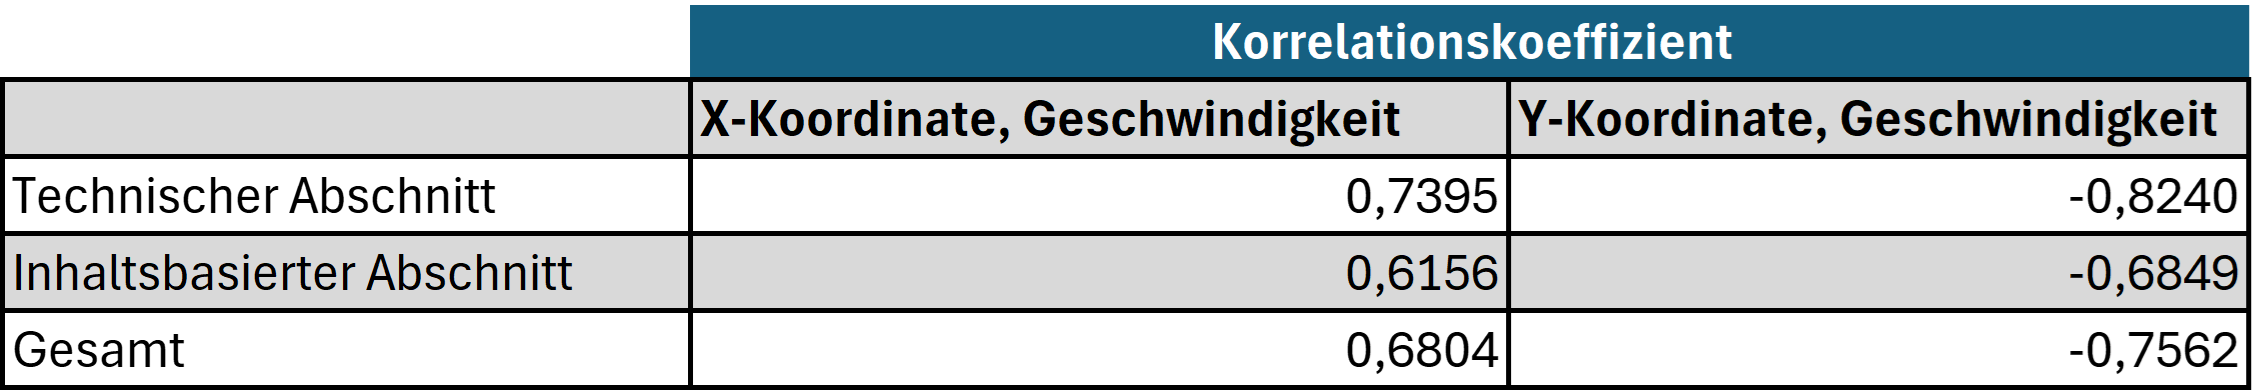
\includegraphics[width=0.95\textwidth]{images/Results/Korrelation-Position-Geschwindigkeit-Table.png}
    \caption{Zusammenhang zwichen der Postion des Objekts im Sichtfeld und der Selektionsgeschwindigkeit beim Cartesian Scanning}
    \label{tab:tableKorrPosGeschwindigkeit}
\end{table}

\begin{figure}
    \centering
    \begin{subfigure}{.5\textwidth}
        \centering
        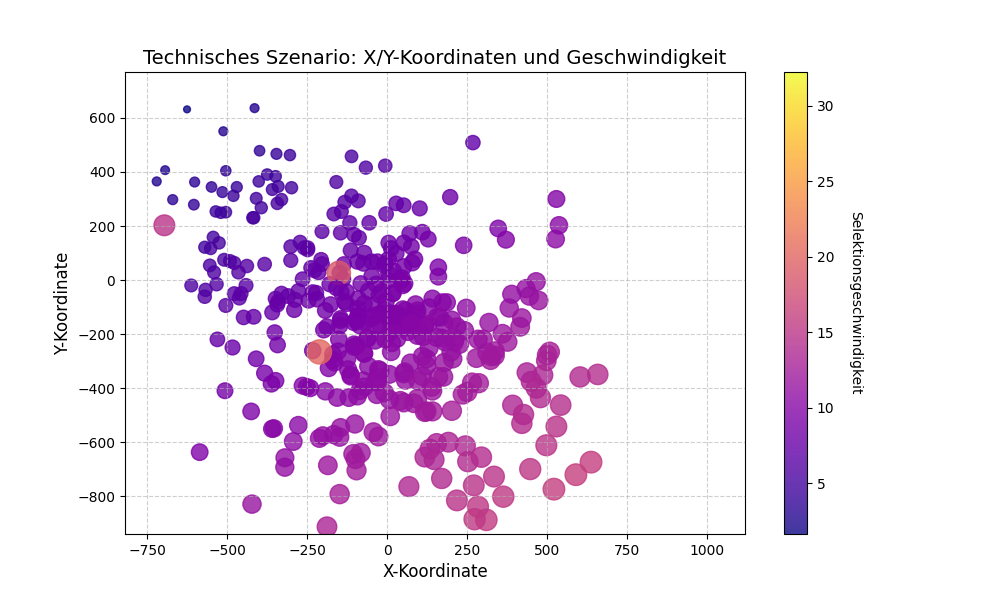
\includegraphics[width=0.95\textwidth]{images/Results/bubbleplot-technisch.png}
        \caption{Technischer Abschnitt}
        \label{fig:bubbleKorrPosGeschwindigkeitTechnisch}
    \end{subfigure}%
    \begin{subfigure}{.5\textwidth}
        \centering
        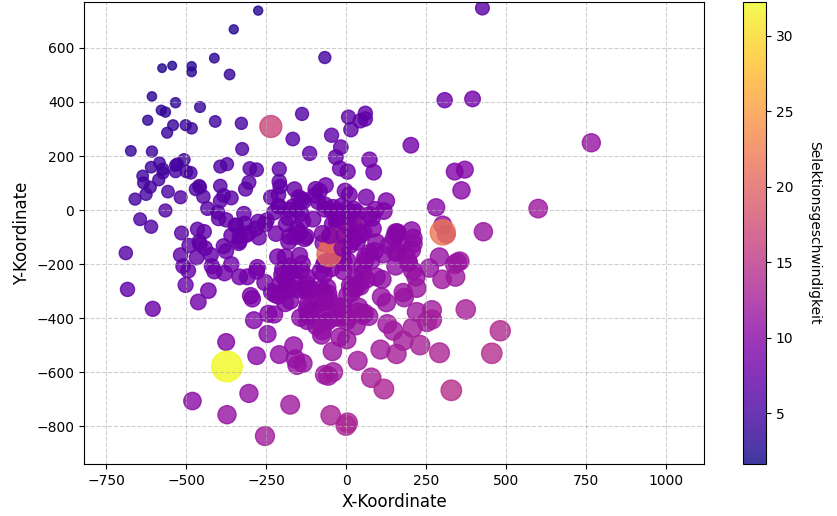
\includegraphics[width=0.95\textwidth]{images/Results/bubbleplot-inhalt.png}
        \caption{Inhaltsbasierter Abschnitt}
        \label{fig:bubbleKorrPosGeschwindigkeitInhalt}
    \end{subfigure}
    \caption{Zusammenhang zwischen der Position des Objektes im Sichtfeld und der Interaktionsgeschwindigkeit beim Cartesain Scanning}
    \label{fig:bubbleKorrPosGeschwindigkeit}
\end{figure}

Für den technischen Abschnitt zeigt sich eine positive Korrelation zwischen der horizontalen Position (x-Koordinate) und der Interaktionsgeschwindigkeit (Korrelationskoeffizient = 0,7395), während die vertikale Position (y-Koordinate) negativ mit der Geschwindigkeit korreliert (Korrelationskoeffizient = -0,8249). Ähnliche Tendenzen lassen sich im inhaltsbasierten Abschnitt beobachten, wo die Korrelationskoeffizienten für die x-Koordinate 0,6156 und für die y-Koordinate -0,6849 betragen. Werden beide Abschnitte zusammen betrachtet, ergeben sich Korrelationskoeffizienten von 0,6804 für die x-Koordinate und -0,7562 für die y-Koordinate. Alle Korrelationen zeigen dabei einen p-Wert <0,00. Die \autoref{fig:bubbleKorrPosGeschwindigkeit} veranschaulicht diese Zusammenhänge. Punkte, die eine schnelle Selektion repräsentieren, befinden sich oben links im Sichtfeld und sind klein und dunkelblau dargestellt. Mit zunehmender Entfernung nach rechts oder unten im Sichtfeld werden die Punkte größer und heller. Darüber hinaus ist in dieser Abbildung zu erkennen, dass die meisten Selektionen in der Mitte des Sichtfeldes durchgeführt wurden.

Anschließend wurde für beide Schnittstellen untersucht, ob es Korrelationen zwischen den Ergebnissen des SSQ und den Bewertungen der SUS, des UEQ und der Interaktionsgeschwindigkeit gibt. Die Ergebnisse dieser Untersuchungen sind in \autoref{tab:tableSymptomsSSQ} dargestellt.

\begin{table}[tbh]
    \centering
    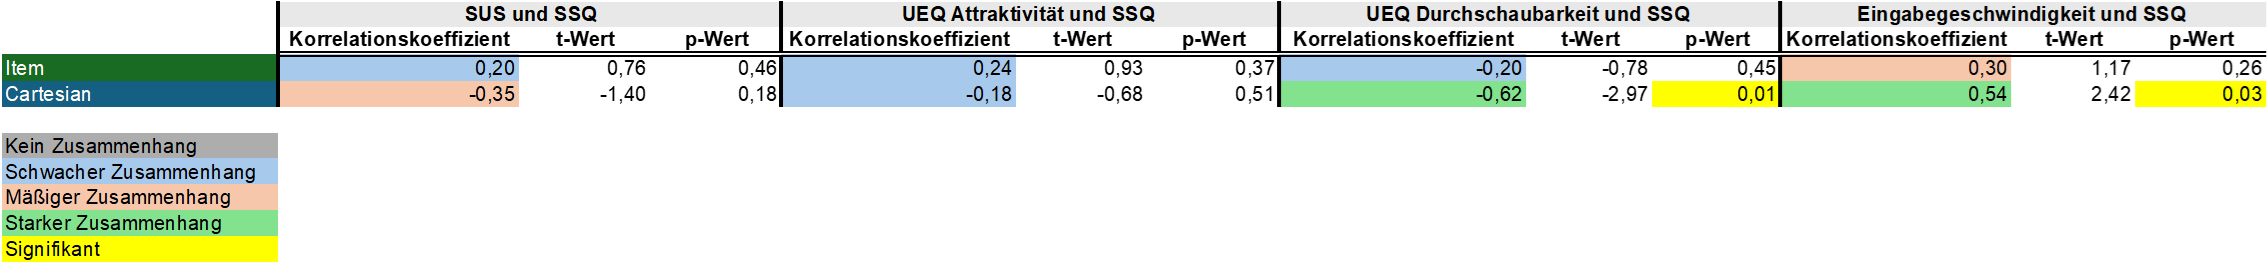
\includegraphics[width=0.95\textwidth]{images/Results/Korrelationen-SSQ.png}
    \caption{Zusammenhänge zwischen den Ergebnissen des SSQ und des SUS, des UEQ sowie der Interaktionsgeschwindigkeit}
    \label{tab:TableKorrelationenSSQ}
\end{table}

Für die Korrelation zwischen SSQ und SUS ergab sich beim Item Scanning ein Korrelationskoeffizient von 0,17 (p-Wert = 0,53), während beim Cartesian Scanning ein Korrelationskoeffizient von -0,33 (p-Wert = 0,21) festgestellt wurde. 

Beim Vergleich des SSQ mit dem UEQ-Faktor Attraktivität ergab sich für das Item Scanning ein Korrelationskoeffizient von 0,24 (p-Wert = 0,36) und für das Cartesian Scanning ein Wert von -0,11 (p-Wert = 0,69). Für den UEQ-Faktor Durchschaubarkeit wurden Korrelationskoeffizienten von -0,20 (p-Wert = 0,45) für das Item Scanning und -0,66 (p-Wert = 0,01) für das Cartesian Scanning berechnet. Der Zusammenhang zwischen dem SSQ und der Interaktionsgeschwindigkeit war beim Item Scanning durch einen Korrelationskoeffizienten von 0,32 (p-Wert = 0,23) und beim Cartesian Scanning durch einen Korrelationskoeffizienten von 0,54 (p-Wert = 0,03) gekennzeichnet.

Darüber hinaus wurden die Zusammenhänge zwischen der Interaktionsgeschwindigkeit im technischen Abschnitt und der Bewertung der SUS sowie zwischen der Interaktionsgeschwindigkeit beider Abschnitte und der Bewertung des UEQ-Faktors Effizienz untersucht. Die Ergebnisse sind in \autoref{tab:TableKorrelationen} dargestellt. 

\begin{table}[tbh]
    \centering
    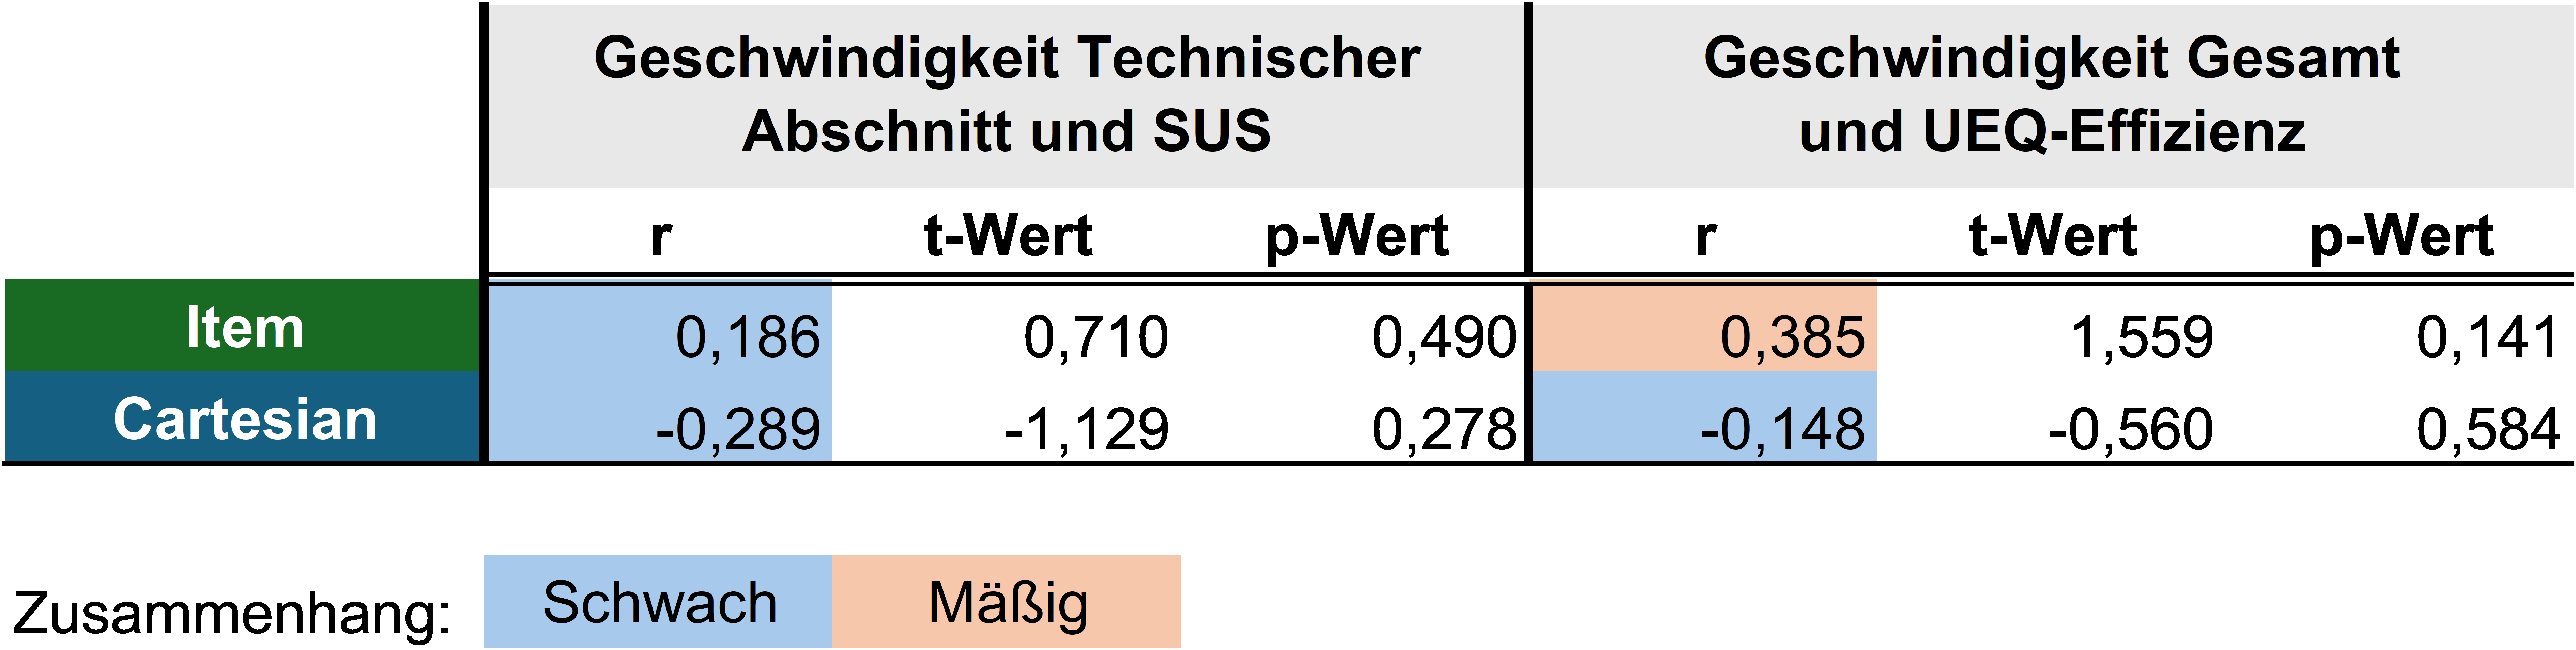
\includegraphics[width=0.95\textwidth]{images/Results/Korrelationen-Rest.png}
    \caption{Zusammenhang zwischen der Interaktionsgeschwindigkeit und der Bewertung der Usability und der UX}
    \label{tab:TableKorrelationen}
\end{table}

Die Korrelationskoeffizienten zwischen der Interaktionsgeschwindigkeit im technischen Abschnitt und dem UEQ-Faktor Effizienz betragen 0,19 (p-Wert = 0,49) für das Item Scanning und -0,29 (p-Wert = 0,28) für das Cartesian Scanning. Für die Interaktionsgeschwindigkeit über alle Abschnitte und den UEQ-Faktor Effizienz wurden Korrelationskoeffizienten von 0,38 (p-Wert = 0,14) für das Item Scanning und -0,15 (p-Wert = 0,58) für das Cartesian Scan errechnet.

\subsection{Qualitative Beobachtungen und Feedback der Teilnehmenden}

Neben den erhobenen Daten wurden während der Evaluation auch Beobachtungen notiert. Besonders auffällig war, dass viele Testpersonen gezielt Kopfbewegungen einsetzten, um das Cartesian Scanning zu beschleunigen oder kleine Fehler zu korrigieren. In \autoref{fig:kopfbewegungenCartesian} ist dargestellt, wie viele Personen gezielte Kopfbewegungen zu welchem Zweck einsetzten. Neun Personen setzten Kopfbewegungen für beide Zwecke ein, vier Personen ausschließlich zur Fehlerkorrektur und eine Person ausschließlich zur Beschleunigung. Zwei Personen setzten keine gezielten Kopfbewegungen ein.

\begin{figure}[tbh]
    \centering
    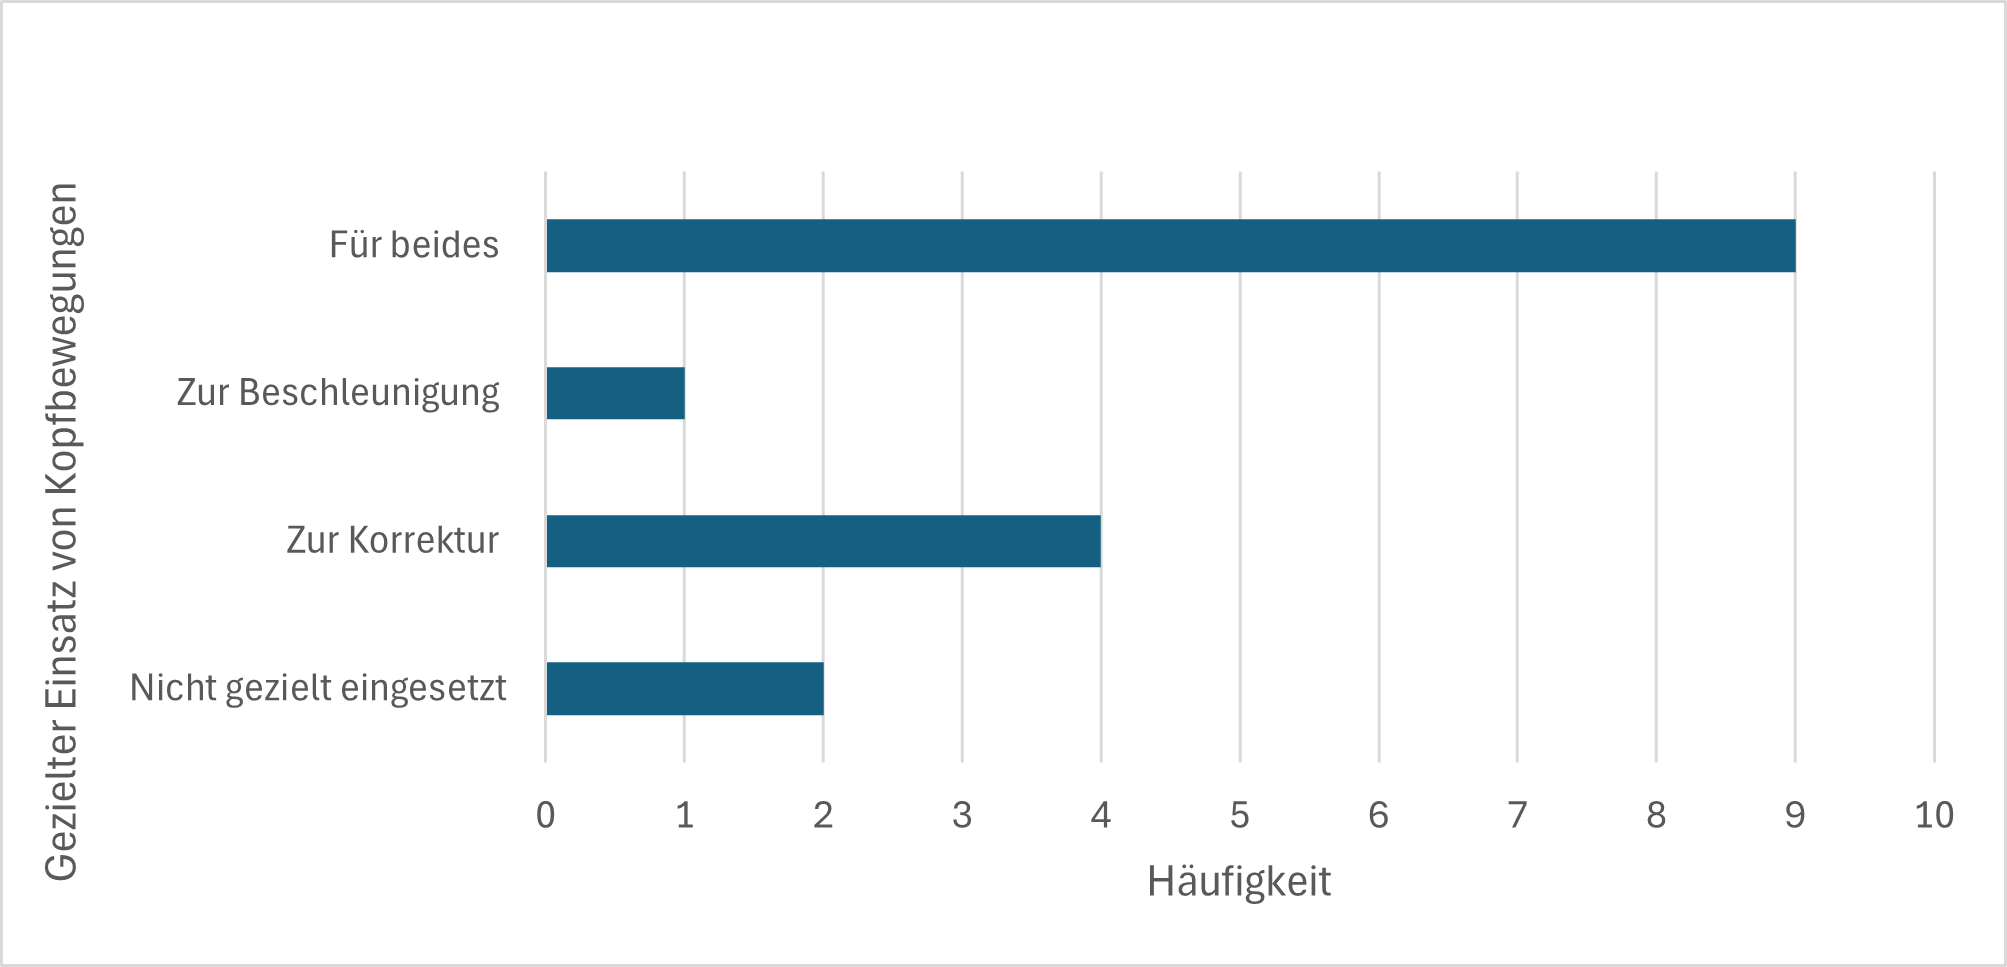
\includegraphics[width=0.8\textwidth]{images/Results/EinsatzKopfbewegungen-Cartesian.png}
    \caption{Einsatz gezielter Kopfbewegungen der Nutzenden beim Cartesian Scanning}
    \label{fig:kopfbewegungenCartesian}
\end{figure}

Darüber hinaus hatten die Teilnehmenden die Möglichkeit, freies Feedback zu den beiden Schnittstellen zu geben. Dieses Feedback wurde kategorisiert und wird im Folgenden zusammengefasst. 

\textbf{Einschätzungen zur Scan Rate:}

Die meisten Testpersonen äußerten sich bezüglich der Scan Rate der beiden Schnittstellen. \autoref{fig:scanrate} gibt die diesbezügliche Einschätzung der Testpersonen wider. Beim Item Scanning empfanden die meisten Testpersonen die Scan Rate als angenehm. Fünf Personen empfanden sie jedoch als zu langsam, eine Person als zu schnell und zwei Personen machten hierzu keine Angabe. Beim Cartesian Scanning empfand keine Person die Scanrate als zu schnell, während sechs Personen sie als angemessen beurteilten. Die meisten Personen gaben an, dass die Scan Rate zu langsam sei. Eine Person äußerte sich nicht.

\begin{figure}[tbh]
    \centering
    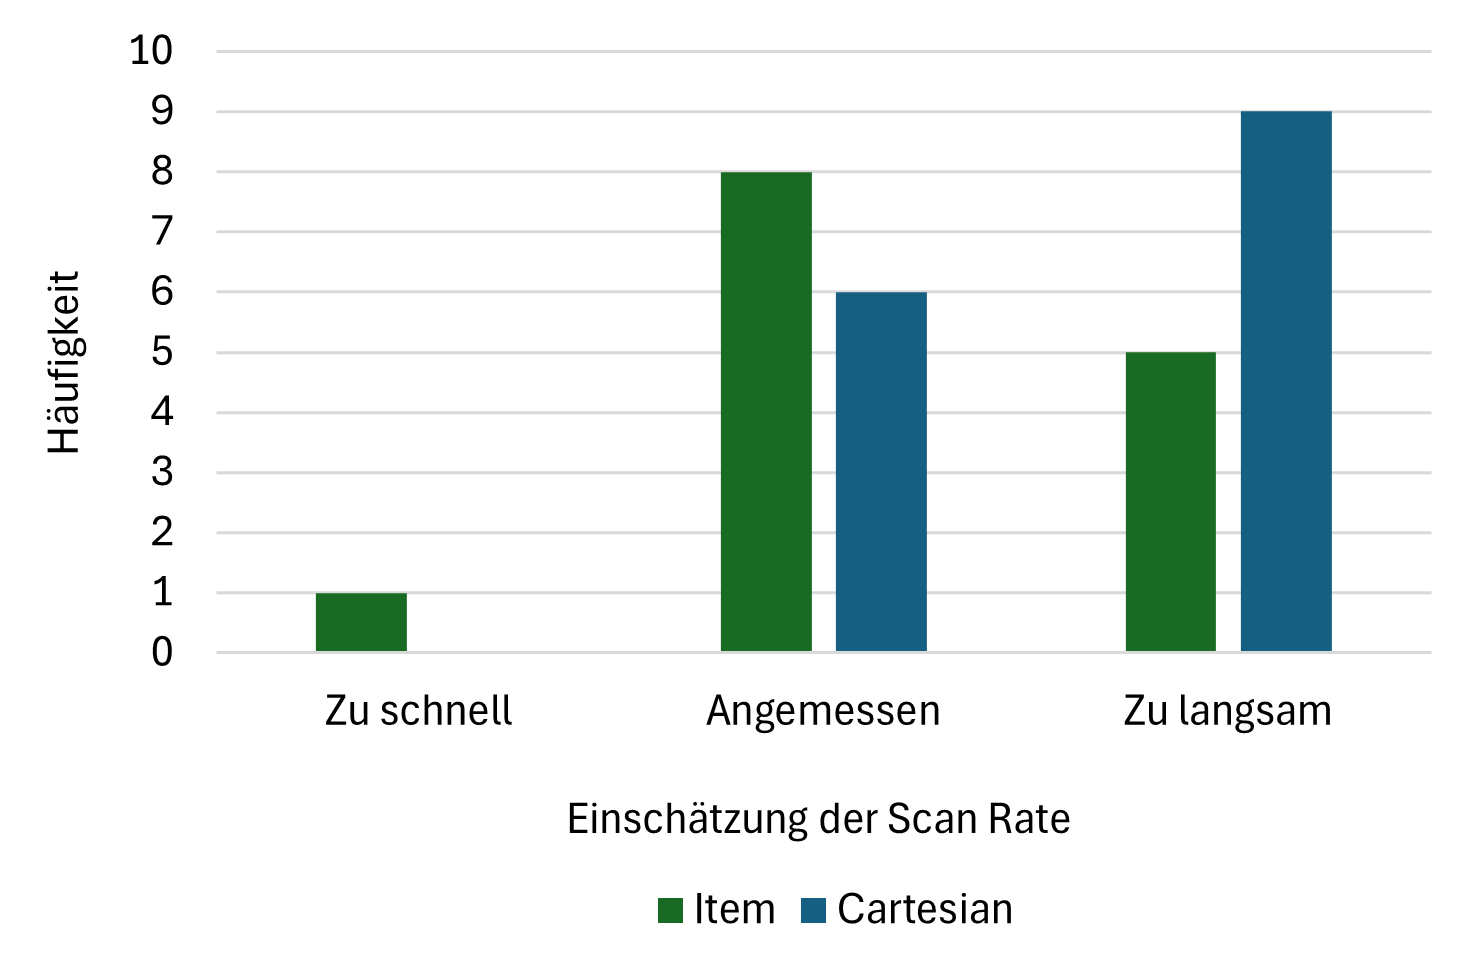
\includegraphics[width=0.75\textwidth]{images/Results/ScanRate.png}
    \caption{Einschätzungen zur Scan Rate beider Interaktionsschnittstellen}
    \label{fig:scanrate}
\end{figure}

\textbf{Probleme und Kritik:}

Die meisten geäußerten Kritikpunkte bzw. Einordnungen der aufgetretenen Probleme bezogen sich auf das Item Scanning. Drei Testpersonen kritisierten die Scanning-Reihenfolge, die als willkürlich oder nicht nachvollziehbar empfunden wurde. Zudem wurde die Animation während des Item Scannings von einer Person als verwirrend beschrieben, da sie dazu führte, dass die Selektion teilweise zu früh erfolgte. Des Weiteren wurde von drei Personen bemängelt, dass das Menü (Navigation und HUD) zu weit oben im Sichtfeld positioniert war. Eine Person äußerte, dass Schwierigkeiten bei der Navigation aufgrund einer zu hohen Scan Rate auftraten. Eine weitere Person merkte an, dass im inhaltsbasierten Abschnitt versteckte Objekte durch das Scanning-Verfahren „gespoilert“ wurden. Dies wurde als schade, aber nicht als ernsthaftes Problem angesehen. 

\textbf{Vorschläge für Verbesserungen:}

Die Testpersonen äußerten verschiedene Ideen zur Verbesserung der Schnittstellen. Beim Item Scanning wurde vorgeschlagen, beim ersten Objekt die Wartezeit etwas zu verlängern, da dieses leicht verpasst werden kann. Außerdem wurde vorgeschlagen, im Navigationsmenü eine Art „Cool Down“ einzuführen, um leichter mehrere Selektionen hintereinander durchführen zu können. Für das Cartesian Scanning wurde vorgeschlagen, die Zeit zu verkürzen, die benötigt wird, um den Schalter für den Moduswechsel gedrückt zu halten. Zwei Personen äußerten auch den Wunsch, die Geschwindigkeit der Linien dynamisch steuern zu können, um Wartezeiten zu reduzieren und das Scanning-Verfahren effizienter zu gestalten. Außerdem wurde vorgeschlagen, die Scan Rate und die Farben für beide Schnittstellen individuell einstellbar zu gestalten.

\textbf{Positives Feedback und Aussagen zu Präferenzen zwischen den Schnittstellen:}

Die Testpersonen gaben auch Feedback zu Aspekten, die sie als positiv empfanden. Die Teilnehmenden beschrieben das Cartesian Scanning als einfacher und lobten die größere Kontrolle über das Scanning. Es wurde auch betont, dass das Cartesian Scanning intuitiver sei. Es wurde außerdem von zwei Testpersonen für die bessere Navigation gelobt, da es einen schnelleren Wechsel des Blickwinkels ermöglichte. Eine Testperson gab an, dass das Cartesian Scanning zwar einfacher und individueller sei, das Item Scanning jedoch mehr Spaß mache. Auch andere Testpersonen bevorzugten das Item Scanning, da es als angenehmer empfunden wurde, insbesondere wegen der schnelleren Interaktionsgeschwindigkeit, der geringeren Fehleranfälligkeit und der optischen Gestaltung, die als augenschonender beschrieben wurde. 



\chapter{Diskussion}
%TO DO für dieses Kapitel: Interpretation bei der Effizienz

In diesem Kapitel werden die Ergebnisse der Evaluation interpretiert und diskutiert, wobei der Fokus darauf liegt, die im Rahmen der Evaluationsplanung formulierten Fragen sowie die Forschungsfrage 3 zu beantworten. Dies umfasst insbesondere die Untersuchung der Unterschiede zwischen den entwickelten Verfahren hinsichtlich der Faktoren Effizienz, Robustheit, Usability, User Experience und Motion Sickness. Dabei wird auch geprüft, ob die erzielten Ergebnisse mit den im Vorfeld formulierten Erwartungen übereinstimmen.

Die Erkenntnisse aus der Analyse der Ergebnisse werden anschließend zusammengefasst, indem die Stärken, Schwächen und Verbesserungsmöglichkeiten der entwickelten Ansätze dargestellt werden. Es wird die Frage beantwortet, welches der beiden Verfahren als geeigneter für den Einsatz in VR eingestuft werden kann. Aufbauend auf diesen Erkenntnissen werden praktische Empfehlungen für die Entwicklung barrierearmer Interaktionsschnittstellen in VR formuliert.

Abschließend wird reflektiert, inwiefern die Zielsetzungen dieser Arbeit erreicht wurden.

\textbf{Effizienz}

Die Effizienz der beiden entwickelten Interaktionsverfahren wurde anhand der Dauer zur Durchführung der Evaluationsabschnitte und der Interaktionsgeschwindigkeit bewertet. Zwischen dem Item Scanning und dem Cartesian Scanning konnten dabei deutliche Unterschiede festgestellt werden.

Zunächst wird betrachtet, wie lang ist die jeweilige Interaktionsgeschwindigkeit beider Verfahren ist und ob ein Verfahren eine deutlich schnellere Interaktionsgeschwindigkeit bietet. Außerdem wird betrachtet, wie lange es im Durchschnitt dauert, die Evaluationsabschnitte zu durchlaufen und ob ein Verfahren dabei einen schnelleren Durchlauf begünstigt. 
Hinsichtlich der Interaktionsgeschwindigkeiten ist zu erkennen, dass das Item Scanning in beiden Evaluationsabschnitten eine deutlich schnellere mittlere Interaktionsgeschwindigkeit aufweist. Darüber hinaus lassen sich bei beiden Verfahren jeweils Unterschiede zwischen der Interaktionsgeschwindigkeit im technischen und im inhaltsbasierten Abschnitt erkennen. Beim Item Scanning ist dieser Unterschied vor allem auf die geringere Anzahl von Objekten in der Szene zurückzuführen, was dazu führt, dass der Scan schneller das gewünschte Ziel erreicht und dieses somit schneller ausgewählt werden kann. Beim Cartesian Scanning lässt sich die etwas schnelle Geschwindigkeit mit der Position der Objekte im Sichtfeld erklären. Im inhaltsbasierten Abschnitt wurden tendenziell mehr Selektionen mittig im Sichtfeld ausgeführt und vergleichend zum technischen Abschnitt weniger weiter unten im Sichtfeld (vgl. \autoref{fig:bubbleKorrPosGeschwindigkeit}).  Dies begünstigt aufgrund der vorliegenden Korrelation zwischen der Interaktionsgeschwindigkeit und der Position des Objekts im Sichtfeld eine schnellere Interaktion. 
Auffallend ist außerdem, dass das Cartesian Scanning eine deutlich größere Spannweite der Interaktionsgeschwindigkeiten aufwies. Dies deutet darauf hin, dass einige Testpersonen mit dem Verfahren vergleichbare Geschwindigkeiten zum Item Scanning erreichen konnten, während andere erheblich länger benötigten. Diese Variabilität kann auf unterschiedliche Nutzungsstrategien zurückgeführt werden, insbesondere auf die gezielte Nutzung von Kopfbewegungen zur Beschleunigung des Scans. Personen, die ihre Kopfbewegungen bewusst einsetzten, konnten ihre Interaktionen dadurch deutlich beschleunigen, während andere ohne diese Strategie langsamer waren. Außerdem variiert die Interaktionsgeschwindigkeit beim Cartesian Scanning stark zwischen Eingaben zur Navigation und Eingaben zur Selektion. Die Navigation wird dabei oft deutlich schneller ausgeführt als die Selektion. Auch dies trägt zu einer höheren Spannweite und Varianz bei. Das Item Scanning hingegen zeigte eine größere Konsistenz zwischen den Testpersonen. Dies liegt insbesondere daran, dass das Verfahren den Nutzenden keine Möglichkeit bietet, die Geschwindigkeit des Scans aktiv zu beeinflussen, vor allem, weil die Nutzenden zwecks der Vergleichbarkeit der Daten nicht die Möglichkeit hatten, die Scan Rate zu verändern. Darüber hinaus ist auch beim Item Scanning erkennbar, dass die Navigation mit schnelleren Interaktionsgeschwindigkeiten einhergeht. So werden bspw. im Navigationsmenü schneller Interaktionen schnell und direkt hintereinander durchgeführt, wenn Nutzende sich mehrfach in eine Richtung drehen möchten. 
Die Unterschiede in der Interaktionsgeschwindigkeit spiegelten sich auch in der Gesamtzeit wider, die die Testpersonen benötigten, um die Evaluationsabschnitte abzuschließen. Für beide Abschnitte benötigten die Teilnehmenden mit dem Cartesian Scanning länger als mit dem Item Scanning, wobei der Unterschied im inhaltsbasierten Szenario besonders deutlich war. Hier waren die Testpersonen waren dem Item Scanning im Mittel über 2 Minuten schneller.  Dies unterstreicht, dass das Item Scanning insbesondere bei Szenen mit wenigen Objekten einen Effizienzvorteil bietet.

Aus diesen Ergebnissen kann geschlossen werden, dass beim Item Scanning insbesondere die Anzahl der Objekte in der Szene als wichtigster Einflussfaktor für die Interaktionsgeschwindigkeit identifiziert werden konnte. Beim Cartesain Scanning lassen sich zwei relevante Einflussfaktoren identifizieren. Dazu zählt zunächst das Ausmaß, in dem Kopfbewegungen zur Beschleunigung des Verfahrens eingesetzt werden.  Je deutlicher und häufiger diese eingesetzt werden, desto schnellere Interaktionsgeschwindigkeiten können erreicht werden. Der zwei Einflussfaktor ist die Position der Objekte im Sichtfeld. Die durchgeführte Korrelationsanalyse hat gezeigt, dass ein signifikanter Zusammenhang zwischen der Interaktionsgeschwindigkeit und der Position vorliegt. Je weiter oben und links sich ein Objekt im Sichtfeld befindet, desto geringer ist die benötigte Zeit zur Selektion. Dies liegt daran, dass die Scanning-Linien entsprechend länger in ihrer Bewegung brauchen, um Objekte weiter rechts oder unten im Sichtfeld zu erreichen. 

Als letztes wurde hinsichtlich der Effizienz untersucht, ob die Interaktionsgeschwindigkeit die wahrgenommene Usability und Effizienz beeinflusst. Für die Usability konnte nur ein schwacher Zusammenhang zwischen der Interaktionsgeschwindigkeit und dem SUS-Score festgestellt werden. Dieser war entsprechend auch statistisch nicht signifikant. Beim Cartesian Scanning zeigte sich eine etwas deutlichere Tendenz, dass längere Interaktionsgeschwindigkeiten mit niedrigeren Usability-Bewertungen in Zusammenhang stehen. Aber auch hier besteht insgesamt nur eine schwache, nicht signifikante Korrelation. 
Hinsichtlich des Zusammenhangs zwischen der Interaktionsgeschwindigkeit und der Bewertung des UEQ-Faktors Effizienz zeigen die Ergebnisse für beide Verfahren unterschiedliche Tendenzen. Während beim Cartesian Scanning nur eine schwache Korrelation bestand, zeigte das Item Scanning eine mäßige, wenn auch statistisch nicht signifikante, Korrelation. Auffällig ist hier, dass es sich um eine positive Korrelation handelt. Das bedeutet, dass langsamere Geschwindigkeiten tendenziell mit besseren Bewertungen der Effizienz einhergehen. %Hier fehlt noch eine Interpretation!! 

\textbf{Robustheit}

Hinsichtlich der Robustheit wurde untersucht, wie häufig Fehler bei der Nutzung der jeweiligen Verfahren auftreten und was die Gründe für diese Fehler sind. Darüber hinaus wurde analysiert, wie viele Zyklen des Scans beim Item Scanning durchschnittlich nötig waren und wie häufig beim Cartesian Scanning leere Eingaben zur Korrektur von Fehlern eingesetzt wurden. 

Beim Item Scanning traten insgesamt Fehler im technischen Abschnitt auf, in dem nur drei Testpersonen fehlerfrei blieben. Die meisten Testpersonen machten hier einen oder mehrere Fehler, die häufig auf Timing-Probleme zurückzuführen waren. Diese resultierten insbesondere aus der Schwierigkeit, den richtigen Zeitpunkt für die Eingabe zu treffen. Dieses Problem trat bei allen Personen auf, die nicht fehlerfrei blieben. Aus der Rückmeldung der Testpersonen lässt sich schließen, dass unter anderem die Animation zwischen den Elementen das Auftreten dieser Fehler begünstigte, da sie zu einer verfrühten Selektion verleitete. Darüber hinaus traten Timing-Probleme verstärkt im Navigationsmenü auf.  Hier kam es oft dazu, dass die Testpersonen eine Navigation durchführten, sich kurz umschauten und im Anschluss eine erneute Navigation in die gleiche Richtung durchführen wollten. Oft wechselte jedoch in diesem Moment der Scan zum nächsten hervorgehobenen Element, wodurch eine Fehlselektion entstand, die eine Navigation in die falsche Richtung auslöste. Mögliche Ansätze, um dem Auftreten dieser Fehler entgegenzuwirken, wären bspw. eine Optimierung der Animation und das Einführen einer längeren Wartezeit auf dem zuvor ausgewählten Objekt im Navigationsmenü. 
Im Rahmen der Gestaltung des technischen Abschnitts für das Item Scanning wurden als Herausforderung eine nicht deutliche Scan-Reihenfolge sowie die Positionierung von Elementen am Rand des Sichtfelds genannt. In der Evaluation traten allerdings keine Fehler auf, die sich auf diese Gründe zurückführen lassen. Längere Wartezeiten bei Zielobjekten, die sich weiter hinten in der Scan-Reihenfolge befinden, haben das Auftreten von Fehlern ebenfalls nicht begünstigt. Auch die Eingabe auf mehreren Ebenen stellte kein Problem dar. 
Beim Cartesian Scanning war das Fehlerprofil vielseitiger. Im technischen Abschnitt blieben mehr Testpersonen fehlerfrei, aber wenn Testpersonen Fehler machten, dann häufig auch zwei oder mehr. Eine der Hauptursachen dafür war die versehentliche Selektion des Hauptmenüs. Wie bereits gezeigt, tendieren die Testpersonen dazu, ihre Blickrichtung so auszurichten, dass die Zielobjekte möglichst mittig im Sichtfeld selektiert werden können. Da das Menü ebenfalls mittig platziert ist, weist es dementsprechend eine räumliche Nähe zu den Zielobjekten auf, was das Auftreten von Selektionsfehlern begünstigt. Außerdem befindet sich das Menü auf der UI-Ebene und damit räumlich näher am Nutzenden. Dadurch wird es von der Implementierung bevorzugt selektiert. Daher können bereits leichte Überdeckungen von Elementen oder Eingaben, die das Zielobjekt in Richtung Menü knapp verfehlen, dazu führen, dass das Menü anstelle des Zielobjekts selektiert wird. 
Ein weiterer häufiger Grund für Fehler stellt das Vergessen des Wechsels des Interaktionsmodus dar. Testpersonen hatten Schwierigkeiten, sich daran zu erinnern, den Modus zu wechseln, bevor sie mit der Interaktion begannen. So wurde meist der Scan gestartet und beim Setzen der ersten Linie erkannt, dass es sich um den falschen Modus handelt. 
Interessanterweise traten keine Fehler auf, die auf die erwartete Schwierigkeit bei der Selektion von Objekten am Rand des Sichtfelds oder nah aneinander liegender Objekte, wie bspw. bei den Antwortmöglichkeiten von Frage-Feldern, zurückzuführen waren. Hierbei ist anzumerken, dass viele Testpersonen diese Herausforderungen jedoch auch durch Anpassung der Blickrichtung über die Navigation oder die Bewegung des Kopfes umgingen. 

Hinsichtlich der Anzahl der benötigten Zyklen beim Item Scanning zusammengefasst werden, dass die meisten Eingaben im ersten Zyklus erfolgten. Das bedeuetet, Elemente wurden meistens direkt ausgewählt, sobald sie erstmalig hervorgehoben wurden. Dabei traten keine großen Unterschiede zwischen den Evaluationsabschnitten auf. Mehrere Zyklen wurden vor allem bei der Navigation benötigt, da sich die Testpersonen oft zunächst orientieren oder bewusst einen weiteren Zyklus abwarteten, um Timing-Fehler zu vermeiden. Dies zeigt, dass die Möglichkeit, mehrere Zyklen zu durchlaufen von den Testpersonen teilweise als bewusste Strategie zur Fehlervermeidung eingesetzt wurde. Die zuvor beschrieben Optionen zur Optimierung der Selektion im Navigationsmenü könnten daher ebenfalls dazu führen, dass die Notwendigkeit von mehreren Zyklen geringer wird.  

Beim Cartesian Scanning stellte die Nutzung von leeren Eingaben eine Strategie zur Korrektur von Fehlern dar. Im technischen Szenario lag der Mittelwert bei einer leeren Eingabe pro Testperson, während im inhaltsbasierten Szenario ein höherer Mittelwert von 1,75 erreicht wurde. Die Spannweite der Nutzung war dabei jedoch recht groß. Während einige Testpersonen diese Option zur Korrektur gar nicht nutzten, griffen andere häufiger darauf zurück, insbesondere wenn zuvor der Wechsel des Interaktionsmodus vergessen wurde. Bei fehlerhaften Setzen der ersten Scan-Linie wurden leere Eingaben hingegen seltender verwendet. Hier versuchten die meisten Testpersonen eher, dies durch gezielte Kopfbewegungen zu korrigieren, anstatt den Prozess durch eine leere Eingabe abzubrechen und neu zu starten. 
Die Ergebnisse zeigen, dass leere Eingaben ein essenzielles Werkzeug zur Fehlerkorrektur darstellen. Ohne diese Option wären vermutlich mehr Fehler aufgetreten. 

\textbf{Erlernbarkeit}

Um zu untersuchen, ob im Verlauf der Evaluation ein messbarer Lerneffekt eingetreten ist, wird analysiert, ob im Verlauf der Evaluation eine Beschleunigung der Interaktionsgeschwindigkeit oder eine Reduktion der Fehleranzahl eingetreten ist.

Beim Item Scanning zeigen die Ergebnisse der durchgeführten linearen Regressionsanalyse, dass die Interaktionsgeschwindigkeit im Verlauf des technischen und im inhaltsbasierten Abschnitt jeweils minimal schneller wird (um 0,839 bzw. 0,391 Sekunden pro Interaktion). Wird die gesamte Evaluation betrachtet, liegt der Effekt bei -2,539 Sekunden und somit deutlich höher. Der Wert wird jedoch durch die geringere Anzahl an Elementen im inhaltsbasierten Abschnitt beeinflusst. Die geringere Anzahl an Elementen hat hier eine geringe Interaktionsgeschwindigkeit begünstigt. Daher ist die Verringerung der Interaktionsgeschwindigkeit über den gesamten Verlauf der Evaluation nicht direkt auf einen Lerneffekt zurückzuführen. Die getrennte Betrachtung der Abschnitte wird daher in diesem Fall als repräsentativer für den Lerneffekt bewertet. Die separate Betrachtung der Entwicklung in den beiden Abschnitten deutet darauf hin, dass keine deutliche Beschleunigung der Interaktionsgeschwindigkeit eingetreten ist, die auf einen Lerneffekt schließen lässt. Die Korrelationskoeffizienten zwischen der Anzahl der getätigten Eingaben und der Interaktionsgeschwindigkeit verdeutlichen dies zusätzlich. Der Zusammenhang ist minimal und im inhaltsbasierten Abschnitt sogar so gering, dass er praktisch keine Bedeutung hat. Dies kann dadurch erklärt werden, dass die Testpersonen beim Item Scanning nicht die Möglichkeit hatten, aktiv Einfluss auf die Geschwindigkeit des Verfahrens zu nehmen, da unter anderem die Scan Rate für alle Personen zwecks Vergleichbarkeit der Ergebnisse festgelegt wurde und nicht anpassbar war. Ein Lerneffekt hätte sich theoretisch darüber hinaus in einer geringeren Anzahl an benötigten Scanning-Zyklen zeigen können, was wiederum zu einer geringeren Interaktionsgeschwindigkeit geführt hätte. Da jedoch die meisten Eingaben jedoch im ersten oder zweiten Durchgang erfolgen, bleibt auch hier nur minimaler Spielraum für eine Verbesserung.
Beim Cartesian Scanning zeigt sich ein noch schwächerer Zusammenhang zwischen der Anzahl getätigter Eingaben und der Interaktionsgeschwindigkeit. Werden die Abschnitte separat betrachtet, verlangsamt sich die Interaktionsgeschwindigkeit tendenziell sogar im Verlauf des Abschnitts (positiver Regressionskoeffizient). Auf die gesamte Evaluation bezogen ist hingegen eine leichte Beschleunigung (um 0,49 Sekunden) erkennbar. Dieser Wert ist hier aussagekräftiger als beim Item Scanning, da beim Cartesian Scanning Faktoren wie die Anzahl der Elemente in der Szene keinen erkennbaren Einfluss auf die Interaktionsgeschwindigkeit haben. Dennoch bestätigen die Korrelationskoeffizienten, dass auch beim Cartesian Scanning praktisch kein signifikanter Zusammenhang besteht, der das Auftreten eines Lerneffekts aufzeigen könnte.

Ein weiteres Indiz für die Erlernbarkeit eines Verfahrens könnte die Reduktion der Fehlerzahl mit zunehmender Erfahrung sein. Die Ergebnisse zur Robustheit zeigen, dass bei beiden Verfahren die Gesamtzahl der Fehler vom technischen zum inhaltsbasierten Abschnitt abnimmt. Dieser Rückgang könnte auf einen Lerneffekt hindeuten. Die höhere Fehlerzahl im technischen Abschnitt könnte jedoch auch mit der höheren Anzahl an Elementen und der bewusst herausfordernden Gestaltung des Abschnitts zusammenhängen, da diese Faktoren das Auftreten von Fehlern in diesem Abschnitt generell begünstigt haben könnten. EEin Lerneffekt kann daher auch in Bezug auf die Fehlerreduktion anhand der vorliegenden Daten nicht sicher nachgewiesen werden. Die Erwartung, dass das Cartesian Scanning eine steilere Lernkurve aufweist, kann daher durch die erhobenen Daten weder bestätigt noch widerlegt werden.

\textbf{Ablenkung durch die Verfahren}

Um zu untersuchen, inwieweit die Nutzung der Verfahren von den Inhalten der VR-Anwendung ablenkt, wurden in Anlehnung an den Presence Questionnaire \citep{witmer_measuring_1998} drei Fragen formuliert. Diese Fragen sollen Aufschluss darüber geben, ob die Verfahren als störend und ablenkend empfunden wurden. 

Die Analyse der Ergebnisse zeigt, dass beide Verfahren in diesem Aspekt überwiegend positiv bewertet und als wenig störend wahrgenommen wurden, wobei das Cartesian Scanning tendenziell etwas besser bewertet wurde.

Die Ergebnisse zeigen, dass sich die Testpersonen bei beiden Verfahren gut auf die Inhalte und Aufgaben in der virtuellen Szene konzentrieren konnten. Dies deutet darauf hin, dass die Interaktionsschnittstellen keine übermäßige kognitive Belastung erzeugten. Das Gefühl, dass die Nutzenden in die virtuelle Umgegung involviert sind, war beim Cartesian Scanning durchschnittlich etwas stärker ausgeprägt. Dies könnte auf eine höhere Immersion und ein verstärktes Gefühl von Presence hinweisen. Die Streuung der Bewertungen war hierbei beim Item Scanning höher, was darauf hindeutet, dass die Wahrnehmung des Verfahrens diesbezüglich stärker von individuellen Präferenzen abhing.

Während beide Verfahren es den Testpersonen ermöglichten, sich auf die Inhalte zu fokussieren, gab es beim Cartesian Scanning diesbezüglich größere Unterschiede zwischen den Personen. Dies deutet darauf hin, dass sich einige Testpersonen stärker auf die Bedienung konzentrieren mussten als andere. 

Insgesamt bestätigen die Ergebnisse, dass beide Verfahren so gestaltet sind, dass sie die Aufmerksamkeit der Nutzenden nicht von den Inhalten ablenken und keine übermäßigen Störungen verursachen. Die Annahme, dass die entwickelten Schnittstellen eine geringe Ablenkung vom Inhalt aufweisen, konnte damit bestätigt werden. Diese Ergebnisse zeigen, dass binäre Interaktionsschnittstellen trotz ihrer Einfachheit so gestaltet werden können, dass sie das Erlebnis nicht wesentlich beeinträchtigen und zugleich ein Gefühl von Presence erzeugt werden kann.

\textbf{Usability}

Die Usability der beiden untersuchten Verfahren wurde von den Testpersonen unterschiedlich bewertet, wobei das Cartesian Scanning im Vergleich zum Item Scanning deutlich besser abschnitt. Die folgenden Einordnungen der SUS-Scores basieren auf den Ergbnissen von \citet{bangor_empirical_2008}. Der SUS-Score des Cartesian Scanning lag mit einem Durchschnitt von 85,63 im Bereich einer guten bis exzellenten Usability, was etwa einer Schulnote „2“ (amerikanisches B) entspricht. Dies deutet darauf hin, dass die Mehrheit der Testpersonen das Verfahren als sehr nutzerfreundlich empfand.
Beim Cartesian Scanning bewerteten 11 von 16 Personen die Usability mit einem Score über 80, was als gut bis exzellent gilt. Sechs dieser Personen erreichten sogar Werte über 92, die mit einer Schulnote „1“ vergleichbar sind. Lediglich zwei Testpersonen vergaben Scores im Bereich zwischen 50 und 60, was als unterdurchschnittlich betrachtet wird und an der Grenze zur Nicht-Akzeptanz liegt. Insgesamt verdeutlich die Verteilung der Scores, dass die Bewertungen recht einheitlich ausfielen und nur wenige Personen Schwierigkeiten bei der Nutzung des Verfahrens hatten.

Im Gegensatz dazu erzielte das Item Scanning einen durchschnittlichen SUS-Score von 73,44, der ebenfalls über dem Durchschnitt liegt, aber nur knapp im Bereich einer guten Usability (Schulnote „3“, amerikanisches C). Die Bewertungen zeigen außerdem eine deutlich größere Streuung der Scores. Während 9 Personen eine Bewertung über 68 (durchschnittliche Usability) vergaben, bewerteten 7 Personen das Verfahren mit einem geringeren Score, wobei 4 Testpersonen sogar Scores unter 60 vergaben, die als mangelhaft oder nicht akzeptabel einzustufen sind. Eine Person bewertete das Verfahren mit einem Score unter 50, was auf eine klare Nicht-Akzeptanz hinweist.

Diese Verteilung deutet darauf hin, dass die Bewertung das Item Scanning stärker von individuellen Präferenzen abhängig ist. Während ein Großteil der Testpersonen die Usability als gut bis sehr gut empfand, gab es auch einen deutlichen Anteil, der das Verfahren als verbesserungswürdig oder gar nicht akzeptabel bewertete.

Insgesamt zeigt die Analyse, dass das Cartesian Scanning hinsichtlich der Usability als überzeugender bewertet wurde. Beim Item Scanning besteht hingegen noch deutlicher Verbesserungsbedarf, um die Usability für alle Anwender:innen auf ein gleichmäßig hohes Niveau zu bringen.

\textbf{User Experience}

Die Evaluation der UX zeigt, dass das Cartesian Scanning in den Faktoren durchschnittlich besser bewertet wurde als das Item Scanning, mit Ausnahme des Faktors Originalität. Beide Verfahren wurden in allen UX-Faktoren durchschnittlich positiv bewertet (Mittelwert >0,8), wobei sich deutliche Unterschiede in den Einzelbewertungen und damit in den Varianzen zeigen.

Beim Cartesian Scanning wurden vor allem die Faktoren Durchschaubarkeit und Attraktivität positiv hervorgehoben, während die Effizienz am schlechtesten bewertet wurde. Die geringeren Varianzen in den Bewertungen zeigen, dass die Testpersonen sich in ihren Einschätzungen weitgehend einig waren, insbesondere in Bezug auf Durchschaubarkeit und Attraktivität. Items, die besonders positiv wahrgenommenen wurden, waren verständlich, leicht zu lernen, angenehm, übersichtlich und aufgeräumt. Trotz der allgemein positiven Rückmeldungen wurde das Item langsam deutlich negativ bewertet, was die geringe Bewertung des Faktor Effizienz bedingt.
Die UX des Item Scanning wurde ebenfalls positiv bewertet, jedoch mit insgesamt größeren Varianzen, was auf stärkere Uneinigkeit unter den Testpersonen hindeutet. Besonders niedrig bewertet wurden die Faktoren Effizienz und Steuerbarkeit. Die niedrigere Bewertung der Steuerbarkeit könnte unter anderem durch die Scan-Reihenfolge bedingt sein. Diese wird durch das System festgelegt und lässt sich nicht aktiv beeinflussen. Insbesondere im technischen Abschnitt empfanden einige Testpersonen die Reihenfolge der Elemente als nicht nachvollziehbar oder nicht erwartungskonform, was aus dem Feedback der Personen hervorgeht. Darüber hinaus könnte auch die geringe Selbstwirksamkeit bzgl. der Interaktionsgeschwindigkeit ein möglicher Grund für die geringere Bewertung des Faktor darstellen. 
Besonders positiv bewertet wurde hingegen der Faktor Originalität. Insbesondere die Items kreativ und neuartig wurden postiv hervorgehoben. Aber auch das Item leicht zu lernen erhilt eine durchaus positive Bewertung. 

Ein zentraler Kritikpunkt bei beiden Verfahren ist die Effizienz, die in beiden Fällen am niedrigsten bewertet wurde. Dies ist verständlich, da Scanning-Verfahren grundsätzlich als langsam zu bewerten sind, insbesondere im Vergleich zu anderen gängien Interaktionsmethoden. Eine Verbessung der Bewertung der Effizienz könnte vermutlich bereits durch eine Einstellung zur Anpassung der Scan Rate erreicht werden. Wie die Ergebnisse aus dem Feedback zeigen, wurde diese von vielen Testpersonen als zu langsam empfunden, inbesondere beim Cartesain Scanning. Eine individuelle Einstellung könnte die wahrgenommene Effizienz deutlich beeinflussen. 
Um die Bewertung der Steuerbarkeit des Item Scannings zu verbessern, könnte neben der Anpassbarkeit der Scan Rate auch die Anpassung der Scan-Reihenfolge. Es wäre denkbar, eine Möglichkeit zu implementieren, die bei Erstellung einer Szene die Option bietet, die Scan-Reihenfolge festzulegen, damit eine nachvollziehbare Lösung für jedes individuelles Szenario geschaffen werden kann. 

Darüber hinaus ist die Zielgruppe ein wichtiger Aspekt für die Einordnung der UX-Bewertungen. Bei den Testpersonen handelte es sich ausschließlich um Personen ohne motorische Beeinträchtigungen, die in ihrem Alltag keine binären Interaktionsschnittstellen nutzen. Daher ist es möglich, dass z.B. Bewertungen zu Faktoren wie Originalität oder Stimulation besonders positiv ausgefallen sind und Personen, die in ihrem Alltag auch Schalter und Scanning-Verfahren nutzen, diese anders bewerten würden. 

Anschließend zur Auswertung des UEQ wurde ergänzend überprüft, inwieweit  die subjektiven Angaben hinsichtlich der Effizienz mit den gemessenen technischen Daten übereinstimmen. Dazu wurde eine Korrelationsanalyse der Bewertung des Faktors Effizenz und der Interaktionsgeschwindigkeit durchgeführt. 
Beim Item Scanning liegt zwischen den Variablen eine mäßige, positive Korrelation vor. Diese zeigt, dass langsamere Interaktionsgeschwindigkeiten tendenziell mit besseren Bewertungen der Effizienz einhergingen. Dieses Ergebnis deutet darauf hin, dass die Bewertung der Effizienz nicht allein durch Geschwindigkeit bestimmt wird und stattdessen viel mehr subjektive Faktoren eine entscheidende Rolle spielen.
Beim Cartesian Scanning wurde nur eine leicht negative Korrelation festgestellt, was bedeutet, dass höhere Geschwindigkeiten tendenziell mit besseren bewertungen der Effizienz zusammenhingen. In diesem Fall scheint die Geschwindigkeit etwas stärker mit der Wahrnehmung von Effizienz verknüpft zu sein als beim Item Scanning. Der Zusammhang ist insgesamt jedoch als recht schwach zu bewerten. Beide Korrelation weisen keine statistische Signifikanz auf, trotzdem verdeutlichen sie, dass eine schnellere Interaktionsgeschwindigkeit kein ausschlaggebender Faktor für die Bewertung der Effizienz ist.

\textbf{Motion Sickness}

Die Evaluation der beiden Verfahren zeigt, dass Motion Sickness Symptome bei beiden Verfahren auftraten, jedoch mit Unterschieden in ihrer Ausprägung und Verteilung. Im Durchschnitt war der SSQ-Score beim Item Scanning leicht höher (12,155) als beim Cartesian Scanning (10,051). Beide Werte weisen auf das Vorhandensein signifikanter Symptome hin, wobei die Verteilung der Scores zwischen den Verfahren variiert. Beim Cartesian Scanning hatten mehr als die Hälfte der Testpersonen (10 Personen) einen Score unter 10, was vernachlässigbaren bis minimalen Symptomen entspricht, während drei Personen einen Score über 20 erreichten, was als besorgniserregend gilt. Beim Item Scanning zeigten hingegen acht Personen einem Score unter 10, während 5 Personen einen Score über 20 aufwiesen. Dies deutet darauf hin, dass insgesamt beim Item Scanning häufiger stärkere Symptome auftraten.

Eine Betrachtung der spezifischen Symptome zeigt, dass in der Kategorie Oculomotor die meisten Symptome auftraten, während in der Kategorie Nausea bei beiden Verfahren die wenigsten Symptome berichtet wurden. Beim Item Scanning berichteten die Testpersonen besonders häufig über angestrengte Augen (11 Personen, davon 4 mit moderater Ausprägung) sowie Ermüdung, Kopfdruck und verschwommenes Sehen. Beim Cartesian Scanning traten ebenfalls häufig angestrengte Augen (11 Personen, davon 2 moderat) sowie leichte Ermüdung (8 Personen) auf, wobei Symptome wie Kopfdruck und verschwommenes Sehen weniger verbreitet waren als beim Item Scanning. Die stärkeren Ausprägung oculomotorischer Symptome bei beiden Verfahren deutet darauf hin, dass beide Verfahren eine kognitive Belastung hervorrufen. 

In der Kategorie Disorientation wurden bei beiden Verfahren die größten Streuungen festgestellt. Während acht Personen beim Item Scanning und neun beim Cartesian Scanning vernachlässigbare Symptome berichteten (Score <5), erreichten einige Testpersonen sehr hohe Scores (>40), was auf erhebliche Einschränlungen hindeutet. Es lässt sich erkennen, dass Disorientation zwar selten, jedoch bei einzelnen Personen besonders ausgeprägt auftreten kann.

Ein entscheidender Einflussfaktor auf die Symptome könnte der Aufbau der Evaluation selbst gewesen sein. Beide Verfahren wurden in einer Sitzung getestet, die 45–60 Minuten dauerte, und erforderten die Erlernung neuer Steuerungen sowie die Bearbeitung vieler Aufgaben. Diese intensive kognitive und visuelle Belastung könnte das Auftreten von oculomotorischen Symptomen wie angestrengte Augen, Ermüdung und Konzentrationsschwierigkeiten begünstigt haben. Dennoch sollte über Optimierungen der Verfahren nachgedacht werden, um die Symptome insgesamt zu reduzieren.

Nach der Auswertung des SSQ wurde untersucht, welche Zusammenhänge zwischen dem Auftreten von Motion Sickness und der Bewertung der Usability und UX sowie der Interaktionsgeschwindigkeit bestehen.
Für die Usability ergab die Korrelationsanalyse beim Item Scanning einen schwachen positiven Zusammenhang. Dies bedeutet, dass höhere SSQ-Scores tendenziell mit einer etwas besseren Bewertung der Berwertung der Usability einhergingen. Beim Cartesian Scanning wurde hingegen ein mäßiger negativer Zusammenhang festgestellt. Hier schienen niedrigere SSQ-Scores zu einer besseren Bewertung der Usability beizutragen. Dies entspricht eher der allgemeinen Erwartung, dass ein Verfahren, das weniger physische oder kognitive Belastungen verursacht, auch als einfacher und angenehmer wahrgenommen wird. Diese Korrelation war jedoch nicht statistisch signifikant. Ein wichtiger Aspekt, der bei der Interpretation dieser Ergebnisse berücksichtigt werden muss, ist der Zeitpunkt der Datenerhebung. Der SUS wurde unmittelbar nach dem technischen Abschnitt ausgefüllt, während der SSQ erst am Ende der Evaluation erhoben wurde. Symptome, die erst während des inhaltsbasierten Abschnitts auftraten, bspw. aufgrund der längeren Nutzungszeit oder erhöhter kognitiver Anforderung, konnten die SUS-Bewertung daher nicht beeinflussen. Dies könnte die positive Korrelation beim Item Scanning erklären und darauf hindeuten, dass ggf. beim Item Scanning die Symptome erst im weiterer Verlauf der Evaluation aufgetreten sind oder sich hier stärker ausgeprägt haben.

Hinsichtlich der UX wurden in der Korrelationsanalyse insbesondere die Faktoren Attraktivität und Durchschaubarkeit betrachtet. 

Beim Cartesian Scanning zeigte sich ein leichter negativer Zusammenhang zwischen dem SSQ Score und der Bewertung der Attraktivität. Dies deutet darauf hin, dass das Verfahren eher als angenehm und sympatisch wahrgenommen wird, wenn weniger körperliche Symptome auftreten. Beim Item Scanning hingegen wurde ein schwacher positiver Zusammenhang festgestellt. Dadurch, dass der Zusammenhang bei beien Verfahren eher schwach ist, kann angenommen werden, dass das Auftreten von Motion Sickness nur einen geringen Einfluss auf die Bewertung der Attraktivität hat und hier andere Faktoren eine wichtigere Rolle einnehmen. 

Ein deutlicherer Zusammenhang besteht zwischen dem SSQ und der UX-Dimension Durchschaubarkeit. Hier wurde bei beiden Verfahren eine negative Korrelation festgestellt, die beim Cartesian Scanning als stark bewertet werden kann und sogar eine statistische Signifikanz aufwies. Dies legt nahe, dass weniger Symptome mit einer besseren Bewertung der Durchschaubarkeit einhergehen. Dies deutet darauf hin, dass ein klar strukturiertes und leicht verständliches Verfahren die Testpersonen weniger belastet und somit weniger Symptome hervorruft. Es wäre aber auch möglich, dass ein Verfahren, das weniger Symptome verursacht, wiederum als übersichtlicher und intuitiver empfunden wird. An dieser Stelle kann die Frage nach der Kausalität entsprechend nicht beantwortet werden. 

Die Korrelationsanalyse zwischen den SSQ-Scores und der Interaktionsgeschwindigkeit zeigt, dass schnellere Interaktionsgeschwindigkeiten tendenziell mit niedrigeren SSQ-Scores und somit weniger Symptomen einhergehen. Beim Cartesian Scanning war dieser Zusammenhang stark und statistisch signifikant, während er beim Item Scanning mäßig ausgeprägt war. Dieser Zusammenhang kann auf zwei Arten interpretiert werden. Einerseits wäre es möglich, dass das Auftreten der Symptome die Interaktionsgeschwindigkeit beeinflusst. Das bedeutet, dass Personen schneller interagieren können, wenn sie weniger Symptome verspüren.. Symptome wie angestrengte Augen, Ermüdung oder Konzentrationsschwierigkeiten könnten die Reaktionszeit und somit die Interaktionsgeschwindigkeit beeinträchtigen. Hinsichtlich des Cartesian Scannings wäre es auch möglich, dass Personen, die Symptome verspüren eher dazu neigen, Kopfbewegungen zu vermeiden, wodurch eine Beschleunigung der Interaktion nicht vorgenommen werden kann. Andererseits könnte auch die Geschwindigkeit die Symptome beeinflussen. Personen, die in der Lage sind, schneller zu interagieren, könnten weniger Symptome entwickeln, da kürzere Interaktionszeiten die okulomotorische und kognitive Belastung verringern könnten.
Beim Item Scanning war die Korrelation schwächer ausgeprägt, was möglicherweise darauf zurückzuführen ist, dass die Interaktionsgeschwindigkeit hier weitgehend durch das System vorgegeben war und nicht aktiv von den Nutzenden beeinflusst werden konnte. Beim Cartesian Scanning hingegen hatten die Testpersonen mehr Kontrolle über die Geschwindigkeit, was zu einer stärkeren Korrelation geführt haben könnte.





Zusammenfassung 
Was sind Stärken der Verfahren (FF3)
Item Scanning:
-	Schnellere Interaktionsgeschwindigkeit, insbesondere bei wenigen Elementen in der Szene 
-	Weniger anfällig für Fehler, robuster 
-	Verfahren lenkt wenig vom Inhalt ab und Personen können sich gut auf die Erfüllung von Aufgaben konzentrieren und nicht auf die Steuerung 
-	Positive Bewertung der UX 
-	Originalität
-	verständlich, kreativ, leicht zu lernen, neuartig
Cartesian:
-	Möglichkeit, dass Verfahren zu beschleunigen mit Kopfbewegungen (sofern das für die Person möglich ist) 
-	Mehr Kontrolle und Selbstwirksamkeit bei diesem Verfahren 
-	Maßnahmen zur Fehlerkorrektur funktionieren und werden genutzt (leere Eingaben, Verschiebung von bereits gesetzter Linie durch Kopfbewegungen) 
-	Verfahren lenkt wenig vom Inhalt ab und Personen können sich gut auf die Erfüllung von Aufgaben konzentrieren und nicht auf die Steuerung; Personen fühlen sich tendenziell etwas mehr involviert 
-	Gute Usability 
-	Positive Bewertung der UX 
-	Hohe Durchschaubarkeit 
-	verständlich, leicht zu lernen, neuartig, angenehm, übersichtlich, aufgeräumt
-	intuitiver 
-	Schnellere Navigation

Wo liegen Schwierigkeiten/verbesserungspotenzial (FF3) 
Item Scanning:
-	Wenig Kontrolle über das Verfahren (Geschwindigkeit und Reihenfolge können nicht beeinflusst werden)
-	Timing-Probleme sind die Hauptursache für Fehler (vgl. genannte Optionen zur Verbesserung) 
-	Verbesserungspotenzial hinsichtlich Usability 
-	Geringe Effizienz und Steuerbarkeit 
-	langsam, nicht erwartungskonform, ineffizient, kompliziert
-	Scan-Reihenfolge oft nicht nachvollziehbar (Verbesserungswürdig - Bei Erstellung einer Szene die Möglichkeit einbauen, die Reihenfolge festzulegen, damit diese nachvollziehbarer ist) 
-	Scan Rate sollte auf jeden Fall einstellbar gemacht werden für mehr Steuerbarkeit und Besserung der Effizienz 
-	Auftreten von tendenziell mehr Motion Sickness Symptomen, insbesondere Ermüdung, Kopfdruck und verschwommenes Sehen
-	Navigationsmenü zu weit oben platziert – Positionierung sollte angepasst werden 
Cartesian Scanning: 
-	Langsam und Geschwindigkeit ist abhängig von Lage des Zielobjekts im Sichtfeld – Meist wird eine mittige Ausrichtung auf das Objekt gewählt – vielleicht sinnvoll, die Linien anders starten zu lassen 
-	Etwas anfälliger für Fehler (geringere Robustheit), vielfältigere Fehler (vgl. genannte Optionen zur Verbesserung) 
-	Geringe Effizienz
-	Motion Sickness Symptome treten bei einigen Personen auf – vor allem Angestrengte Augen und Ermüdung
-	Scan Rate etwas zu langsam gewählt – einstellbar machen 
-	Zeit zum gedrückt halten des Schalters beim Wechsel des Modus etwas zu lang 
-	Die meisten Interaktionen finden beim Cartesian in der Mitte statt (Ausrichtung des gewünschten Objekts in der Mitte des Sichtfelds) --> Überlegung die Bewegung des Scans so zu gestalten, dass dieser die Mitte schneller erreicht. Dadurch könnte die Geschwindigkeit optimiert werden 


Ist ein Verfahren geeigneter für VR? (FF3) 
-	Beide Verfahren haben Vor- und Nachteile bzw. zeigen in der aktuellen Gestaltung und Implementierung noch Verbesserungspotenzial auf 
-	Cartesian wurde insgesamt besser und einheitlicher bewertet 
-	Beim Item gingen die Bewertungen öfter stärker auseinander 
-	Insbesondere das freie Feedback zeigt, dass es (trotz besserer Bewertung des Cartesian Scanning) einige Testpersonen gab, die das Item Scanning bevorzugten
-	Im aktuellen Zustand der Implementierung lässt sich sagen, dass das Cartesian Scanning etwas besser angenommen wird 
-	Allerdings zeigen die Ergebnisse, dass beide Verfahren Potenzial für den Einsatz in VR haben und es sich lohnt, die Entwicklung beider Verfahren weiter zu verfolgen und die Verfahren zu optimieren 
-	Ergebnisse deuten darauf hin, dass viel auf persönlichen Präferenzen basiert, wodurch nicht klar gesagt werden kann, dass sich ein Verfahren grundsätzlich besser für den Einsatz in VR eignet 
Ableitung von Empfehlungen (FF4) 
-	Bei Cartesain Positionierung berücksichtigen (unten rechts vermeiden), mitte wird bevorzugt 
-	Bei Item Scanning möglichst wenig Objekte einbinden 
Inwiefern wurden die Zielsetzungen der Arbeit erfüllt 
-	Ziele werden als erfüllt betrachtet 
-	Es wurden die Interaktionsschnittstellen implementiert und hinsichtlich vieler Aspekte evaluiert 
-	Ergebnisse bieten Grundlage für Verbesserungen und zukünftige Entwicklungen  

Außerdem (auf alle Ergebnisse bezogen):
-	Nur recht kleine Anzahl an Teilnehmenden, daher können die Ergebnisse zu Tendenzen aufzeigen 
-	Statistische Signifikanz ist bei der kleinen Anzahl an Testpersonen nicht so leicht zu erreichen 




\section{Ausblick}
Hier wird reflektiert, in welchem Umfang die Zielsetzungen der Arbeit erreicht werden konnten. In der Regel gelingt dies durch den Bezug auf die Evaluation.

Typischer Umfang: 1-2 Seiten.



Manchmal konnte im Rahmen einer Bachelor- oder Masterarbeit ein
wissenschaftliches Thema auch so tief bearbeitet werden, dass wir es auf einem
wissenschaftlichen Workshop oder einer Konferenz veröffentlichen konnten.

Für Themen aus dem Bereich Virtuelle oder Erweiterte Realität bietet sich dazu
zum Beispiel der jährlich stattfindende Workshop der Fachgruppe VR/AR der
Gesellschaft für Informatik an. \citet{Bluhm:Sonar:2009} ist nur ein Beispiel
von mehreren Veröffentlichungen aus unserer Gruppe.





\bibliographystyle{plainnat}
\bibliography{literature}

% Anhang
\appendix
%&%\chapter*{Anhang} % Ein Kapitel ohne Nummerierung
\addcontentsline{toc}{chapter}{Anhang} % Fügt das Anhang-Kapitel dem Inhaltsverzeichnis hinzu
%\addchap{Anhang}

\chapter{Test-Anhang}
% Versicherung bei Diplomarbeiten...

\section{Unity Projekt}
\label{Anhang:Projekt}

\section{Evaluation}

\subsection{Screenshots aus den technischen Szenarien}
\label{Anhang:screenTechnisch}
\subsection{Screenshots aus den inhaltsbasieren Szenarien}
\label{Anhang:screenInhalt}
\subsection{Evaluationsprotokoll}
\label{Anhang:protokoll}

\cleardoublepage

\chapter{Test-Anhang 2}

Test

\cleardoublepage


% Anhang des Dokuments
\backmatter

\chapter{Erklärung}

Soweit meine Rechte berührt sind, erkläre ich mich einverstanden, dass die vorliegende Arbeit Angehörigen der Hochschule Emden/Leer für Studium / Lehre / Forschung unein-geschränkt zugänglich gemacht werden kann.

\vspace{2cm}

% Damit beide Kapitel auf einer Seite stehen
{\let\clearpage\relax\chapter{Eidesstaatliche Versicherung}}

Ich, die Unterzeichnende, erkläre hiermit an Eides statt, dass ich die vorliegende Arbeit selbständig verfasst habe und keine anderen als die angegebenen Quellen und Hilfsmit-tel benutzt habe. Alle Quellenangaben und Zitate sind richtig und vollständig wiederge-geben und in den jeweiligen Kapiteln und im Literaturverzeichnis wiedergegeben. Die vorliegende Arbeit wurde nicht in dieser oder einer ähnlichen Form ganz oder in Teilen zur Erlangung eines akademischen Abschlussgrades oder einer anderen Prüfungsleistung eingereicht.\\

Mir ist bekannt, dass falsche Angaben im Zusammenhang mit dieser Erklärung straf-rechtlich verfolgt werden können.

\vspace{2cm}

\myOrt, den \myDate

\vspace{1cm}

\myAuthor


\end{document}
